\documentclass[11pt,a4paper,dvipsnames,twosided]{article}
\usepackage[deliverable]{IOHKCoverPage}

% data for Deliverable header -- added by KH from an EU H2020 project template
\DeliverableNumber{SL-D5}
\DeliverableTitle{A Formal Specification of the Cardano Ledger}{Formal Cardano Ledger Spec.}
\DeliverableResponsible{Formal Methods Team}
\EditorName{Jared Corduan, \IOHK}
\Authors{Jared Corduan \quad \texttt{<jared.corduan@iohk.io>}
   \\[1em]
   Polina Vinogradova \quad \texttt{<polina.vinogradova@iohk.io>}
   \\[1em]
   Matthias G\"udemann \quad \texttt{<matthias.gudemann@iohk.io>}
}
\DueDate{15$^{\textrm{th}}$ October 2019}
\SubmissionDate{8th October 2019}{2019/10/08}
\LeaderName{Philipp Kant, \IOHK}
\InstitutionAddress{\IOHK}
\Version{1.0}
\Project{Shelley Ledger}
\DisseminationPU

\usepackage[margin=2.5cm]{geometry}
\usepackage{lscape}
\usepackage{iohk}
\usepackage{microtype}
\usepackage{mathpazo} % nice fonts
\usepackage{amsmath}
\usepackage{amssymb}
\usepackage{amsthm}
\usepackage{latexsym}
\usepackage{mathtools}
\usepackage{stmaryrd}
\usepackage{extarrows}
\usepackage{slashed}
\usepackage[unicode=true,pdftex,pdfa,colorlinks=true]{hyperref}
\usepackage{xcolor}
\usepackage[capitalise,noabbrev,nameinlink]{cleveref}
\usepackage{float}
\floatstyle{boxed}
\restylefloat{figure}
\usepackage{tikz}
\usepackage{booktabs}
\usepackage{enumerate}
\usepackage{listings}
%%
%% Package `semantic` can be used for writing inference rules.
%%
\usepackage{semantic}
%% Setup for the semantic package
\setpremisesspace{20pt}

\usepackage{tocloft}
\addtolength{\cftsubsecnumwidth}{5pt}

%%
%% Types
%%
\newcommand{\Nothing}{\ensuremath{\Diamond}}
\newcommand{\N}{\ensuremath{\mathbb{N}}}
\newcommand{\Bool}{\type{Bool}}
\newcommand{\Npos}{\ensuremath{\mathbb{N}^{>0}}}
\newcommand{\Z}{\ensuremath{\mathbb{Z}}}
\newcommand{\Q}{\ensuremath{\mathbb{Q}}}
\newcommand{\R}{\ensuremath{\mathbb{R}}}
\newcommand{\Rnn}{\ensuremath{\mathbb{R}^{\geq 0}}}
\newcommand{\Tx}{\type{Tx}}
\newcommand{\TxBody}{\type{TxBody}}
\newcommand{\TxWitness}{\type{TxWitness}}
\newcommand{\Ix}{\type{Ix}}
\newcommand{\TxId}{\type{TxId}}
\newcommand{\Addr}{\type{Addr}}
\newcommand{\UTxO}{\type{UTxO}}
\newcommand{\Wdrl}{\type{Wdrl}}
\newcommand{\Coin}{\type{Coin}}
\newcommand{\PParams}{\type{PParams}}
\newcommand{\PParamsUpdate}{\type{PParamsUpdate}}
\newcommand{\ProposedPPUpdates}{\type{ProposedPPUpdates}}
\newcommand{\Slot}{\type{Slot}}
\newcommand{\StabilityWindow}{\ensuremath{\mathsf{StabilityWindow}}}
\newcommand{\RandomnessStabilisationWindow}{\ensuremath{\mathsf{RandomnessStabilisationWindow}}}
\newcommand{\SlotsPerEpoch}{\mathsf{SlotsPerEpoch}}
\newcommand{\SlotsPerKESPeriod}{\mathsf{SlotsPerKESPeriod}}
\newcommand{\MaxMajorPV}{\mathsf{MaxMajorPV}}
\newcommand{\ActiveSlotCoeff}{\mathsf{ActiveSlotCoeff}}
\newcommand{\Network}{\mathsf{Network}}
\newcommand{\NetworkId}{\mathsf{NetworkId}}
\newcommand{\BlockNo}{\type{BlockNo}}
\newcommand{\MaxKESEvo}{\ensuremath{\mathsf{MaxKESEvo}}}
\newcommand{\Quorum}{\ensuremath{\mathsf{Quorum}}}
\newcommand{\MaxLovelaceSupply}{\ensuremath{\mathsf{MaxLovelaceSupply}}}
\newcommand{\Duration}{\type{Duration}}
\newcommand{\StakePools}{\type{StakePools}}
\newcommand{\Seed}{\type{Seed}}
\newcommand{\seedOp}{\star}
\newcommand{\Ppm}{\type{Ppm}}
\newcommand{\ProtVer}{\ensuremath{\type{ProtVer}}}
\newcommand{\Metadatum}{\ensuremath{\type{Metadatum}}}
\newcommand{\Metadata}{\ensuremath{\type{Metadata}}}
\newcommand{\MetadataHash}{\ensuremath{\type{MetadataHash}}}
\newcommand{\Update}{\type{Update}}
\newcommand{\GenesisDelegation}{\type{GenesisDelegation}}
\newcommand{\FutGenesisDelegation}{\type{FutGenesisDelegation}}

\newcommand{\DCert}{\type{DCert}}
\newcommand{\DCertRegKey}{\type{DCert_{regkey}}}
\newcommand{\DCertDeRegKey}{\type{DCert_{deregkey}}}
\newcommand{\DCertDeleg}{\type{DCert_{delegate}}}
\newcommand{\DCertRegPool}{\type{DCert_{regpool}}}
\newcommand{\DCertRetirePool}{\type{DCert_{retirepool}}}
\newcommand{\DCertGen}{\type{DCert_{genesis}}}
\newcommand{\DCertMir}{\type{DCert_{mir}}}
\newcommand{\PoolParam}{\type{PoolParam}}
\newcommand{\PoolMD}{\type{PoolMD}}
\newcommand{\MIRPot}{\type{MIRPot}}
\newcommand{\InstantaneousRewards}{\type{InstantaneousRewards}}
\newcommand{\ReservesMIR}{\type{ReservesMIR}}
\newcommand{\TreasuryMIR}{\type{TreasuryMIR}}
\newcommand{\URL}{\type{Url}}
\newcommand{\UTxOState}{\ensuremath{\type{UTxOState}}}
\newcommand{\ledgerState}{\ensuremath{\type{ledgerState}}}

\newcommand{\AddrRWD}{\type{Addr_{rwd}}}
\newcommand{\AddrB}{\type{Addr_{base}}}
\newcommand{\AddrP}{\type{Addr_{ptr}}}
\newcommand{\AddrE}{\type{Addr_{enterprise}}}
\newcommand{\AddrBS}{\type{Addr_{bootstrap}}}
\newcommand{\Ptr}{\type{Ptr}}
\newcommand{\DState}{\type{DState}}
\newcommand{\DWEnv}{\type{DWEnv}}
\newcommand{\DPSEnv}{\type{DPSEnv}}
\newcommand{\DPEnv}{\type{DPEnv}}
\newcommand{\DEnv}{\type{DEnv}}
\newcommand{\PEnv}{\type{PEnv}}
\newcommand{\DPState}{\type{DPState}}
\newcommand{\PState}{\type{PState}}
\newcommand{\DCertBody}{\type{DCertBody}}
\newcommand{\TData}{\type{TData}}
\newcommand{\DPoolReap}{\ensuremath{\type{poolreap}}}
\newcommand{\UPIState}{\type{UPIState}}
\newcommand{\UpdatePayload}{\type{UpdatePayload}}

% multi-signature
\newcommand{\StakeCredential}{\type{Credential}_{stake}}

\newcommand{\txwitsVKey}[1]{\fun{txwitsVKey}~\var{#1}}
\newcommand{\txwitsScript}[1]{\fun{txwitsScript}~\var{#1}}

\newcommand{\AddrVKey}{\type{Addr^{vkey}}}
\newcommand{\AddrRWDVKey}{\type{Addr_{rwd}^{vkey}}}
\newcommand{\AddrRWDScr}{\type{Addr_{rwd}^{script}}}
\newcommand{\AddrVKeyB}{\type{Addr^{vkey}_{base}}}
\newcommand{\AddrVKeyP}{\type{Addr^{vkey}_{ptr}}}
\newcommand{\AddrVKeyE}{\type{Addr^{vkey}_{enterprise}}}
\newcommand{\AddrVKeyBS}{\type{Addr^{vkey}_{bootstrap}}}
\newcommand{\AddrScr}{\type{Addr^{script}}}
\newcommand{\AddrScrBase}{\type{Addr_{base}^{script}}}
\newcommand{\AddrScrEnterprise}{\type{Addr_{enterprise}^{script}}}
\newcommand{\AddrScrPtr}{\type{Addr_{ptr}^{script}}}
\newcommand{\HashScr}{\type{ScriptHash}}
\newcommand{\Script}{\type{Script}}
\newcommand{\MSig}{\type{MSig}}
\newcommand{\Credential}{\type{Credential}}

%% Adding witnesses
\newcommand{\TxIn}{\type{TxIn}}
\newcommand{\TxOut}{\type{TxOut}}
\newcommand{\VKey}{\type{VKey}}
\newcommand{\VKeyEv}{\type{VKey_{ev}}}
\newcommand{\VKeyGen}{\type{VKey_G}}
\newcommand{\SKey}{\type{SKey}}
\newcommand{\SKeyEv}{\type{SKey_{ev}}}
\newcommand{\KeyHash}{\type{KeyHash}}
\newcommand{\KeyHashGen}{\type{KeyHash_G}}
\newcommand{\KeyPair}{\type{KeyPair}}
\newcommand{\KeyPairEv}{\type{KeyPair_{ev}}}
\newcommand{\Sig}{\type{Sig}}
\newcommand{\Data}{\type{Data}}
\newcommand{\Ser}{\type{Ser}}
%% Adding delegation
\newcommand{\Epoch}{\type{Epoch}}
\newcommand{\KESPeriod}{\type{KESPeriod}}
%% Blockchain
\newcommand{\Acnt}{\type{Acnt}}
\newcommand{\Gkeys}{\var{G_{keys}}}
\newcommand{\Block}{\type{Block}}
\newcommand{\SlotId}{\type{SlotId}}
\newcommand{\PPUpdateState}{\type{PPUpdateState}}
\newcommand{\PPUpdateEnv}{\type{PPUpdateEnv}}
\newcommand{\UTxOEnv}{\type{UTxOEnv}}
\newcommand{\CEEnv}{\type{CEEnv}}
\newcommand{\CEState}{\type{CEState}}
\newcommand{\BDEnv}{\type{BDEnv}}
\newcommand{\BDState}{\type{BDState}}
\newcommand{\LEnv}{\type{LEnv}}
\newcommand{\LState}{\type{LState}}

\newcommand{\Proof}{\type{Proof}}
\newcommand{\Seedl}{\mathsf{Seed}_\ell}
\newcommand{\Seede}{\mathsf{Seed}_\eta}
\newcommand{\slotToSeed}[1]{\fun{slotToSeed}~ \var{#1}}
\newcommand{\prevHashToNonce}[1]{\fun{prevHashToNonce}~ \var{#1}}
\newcommand{\isOverlaySlot}[3]{\fun{isOverlaySlot}~\var{#1}~\var{#2}~\var{#3}}
\newcommand{\classifyOverlaySlot}[5]{\fun{classifyOverlaySlot}~\var{#1}~\var{#2}~\var{#3}~\var{#4}~\var{#5}}

\newcommand{\T}{\type{T}}
\newcommand{\vrf}[3]{\fun{vrf}_{#1} ~ #2 ~ #3}
\newcommand{\verifyVrf}[4]{\fun{verifyVrf}_{#1} ~ #2 ~ #3 ~#4}

\newcommand{\HashHeader}{\type{HashHeader}}
\newcommand{\HashBBody}{\type{HashBBody}}
\newcommand{\bhHash}[1]{\fun{bhHash}~ \var{#1}}
\newcommand{\bHeaderSize}[1]{\fun{bHeaderSize}~ \var{#1}}
\newcommand{\bSize}[1]{\fun{bSize}~ \var{#1}}
\newcommand{\bBodySize}[1]{\fun{bBodySize}~ \var{#1}}
\newcommand{\OCert}{\type{OCert}}
\newcommand{\BHeader}{\type{BHeader}}
\newcommand{\BHBody}{\type{BHBody}}

\newcommand{\bheader}[1]{\fun{bheader}~\var{#1}}
\newcommand{\hsig}[1]{\fun{hsig}~\var{#1}}
\newcommand{\bprev}[1]{\fun{bprev}~\var{#1}}
\newcommand{\bhash}[1]{\fun{bhash}~\var{#1}}
\newcommand{\bvkcold}[1]{\fun{bvkcold}~\var{#1}}
\newcommand{\bseedl}[1]{\fun{bseed}_{\ell}~\var{#1}}
\newcommand{\bprfn}[1]{\fun{bprf}_{n}~\var{#1}}
\newcommand{\bseedn}[1]{\fun{bseed}_{n}~\var{#1}}
\newcommand{\bprfl}[1]{\fun{bprf}_{\ell}~\var{#1}}
\newcommand{\bocert}[1]{\fun{bocert}~\var{#1}}
\newcommand{\bnonce}[1]{\fun{bnonce}~\var{#1}}
\newcommand{\bleader}[1]{\fun{bleader}~\var{#1}}
\newcommand{\hBbsize}[1]{\fun{hBbsize}~\var{#1}}
\newcommand{\bbodyhash}[1]{\fun{bbodyhash}~\var{#1}}
\newcommand{\overlaySchedule}[3]{\fun{overlaySchedule}~\var{#1}~\var{#2}~\var{#3}}

\newcommand{\OCertEnv}{\type{OCertEnv}}
\newcommand{\PrtclState}{\type{PrtclState}}
\newcommand{\PrtclEnv}{\type{PrtclEnv}}
\newcommand{\OverlayEnv}{\type{OverlayEnv}}
\newcommand{\VRFState}{\type{VRFState}}
\newcommand{\TickNonceState}{\type{TickNonceState}}
\newcommand{\TickNonceEnv}{\type{TickNonceEnv}}
\newcommand{\NewEpochState}{\type{NewEpochState}}
\newcommand{\UpdateNonceState}{\type{UpdateNonceState}}
\newcommand{\UpdateNonceEnv}{\type{UpdateNonceEnv}}
\newcommand{\PoolDistr}{\type{PoolDistr}}
\newcommand{\BBodyEnv}{\type{BBodyEnv}}
\newcommand{\BBodyState}{\type{BBodyState}}
\newcommand{\RUpdEnv}{\type{RUpdEnv}}
\newcommand{\ChainEnv}{\type{ChainEnv}}
\newcommand{\ChainState}{\type{ChainState}}
\newcommand{\ChainSig}{\type{ChainSig}}
\newcommand{\LastAppliedBlock}{\type{LastAppliedBlock}}
\newcommand{\lastAppliedHash}[1]{\fun{lastAppliedHash}~\var{#1}}


%%
%% Functions
%%
\newcommand{\txins}[1]{\fun{txins}~ \var{#1}}
\newcommand{\txouts}[1]{\fun{txouts}~ \var{#1}}
\newcommand{\txcerts}[1]{\fun{txcerts}~ \var{#1}}
\newcommand{\txid}[1]{\fun{txid}~ \var{#1}}
\newcommand{\outs}[1]{\fun{outs}~ \var{#1}}
\newcommand{\values}[1]{\fun{values}~ #1}
\newcommand{\ubalance}[1]{\fun{ubalance}~ \var{#1}}
\newcommand{\txttl}[1]{\fun{txttl}~ \var{#1}}
\newcommand{\firstSlot}[1]{\fun{firstSlot}~ \var{#1}}
\newcommand{\totalDeposits}[3]{\fun{totalDeposits}~ \var{#1} ~ \var{#2} ~ \var{#3}}
\newcommand{\keyRefund}[6]{\fun{keyRefund}~ {#1}~{#2}~{#3}~\var{#4}~\var{#5}~\var{#6}}
\newcommand{\refund}[4]{\fun{refund}~ \var{#1}~ \var{#2}~ {#3}~ {#4}}
\newcommand{\keyRefunds}[2]{\fun{keyRefunds}~ \var{#1}~ \var{#2}}
\newcommand{\consumed}[2]{\fun{consumed}~ \var{#1}~ \var{#2}}
\newcommand{\produced}[2]{\fun{produced}~ \var{#1}~ \var{#2}}
\newcommand{\applyFun}[2]{\fun{#1}~\var{#2}}

\newcommand{\RegKey}[1]{\textsc{RegKey}(#1)}
\newcommand{\DeregKey}[1]{\textsc{DeregKey}(#1)}
\newcommand{\Delegate}[1]{\textsc{Delegate}(#1)}
\newcommand{\RegPool}[1]{\textsc{RegPool}(#1)}
\newcommand{\RetirePool}[1]{\textsc{RetirePool}(#1)}
\newcommand{\cwitness}[1]{\fun{cwitness}~ \var{#1}}
\newcommand{\dpool}[1]{\fun{dpool}~ \var{#1}}
\newcommand{\poolParam}[1]{\fun{poolParam}~ \var{#1}}
\newcommand{\retire}[1]{\fun{retire}~ \var{#1}}
\newcommand{\addrRw}[1]{\fun{addr_{rwd}}~ \var{#1}}
\newcommand{\epoch}[1]{\fun{epoch}~\var{#1}}
\newcommand{\kesPeriod}[1]{\fun{kesPeriod}~\var{#1}}

%% UTxO witnesses
\newcommand{\inputs}[1]{\fun{inputs}~ \var{#1}}
\newcommand{\txwits}[1]{\fun{txwits}~ \var{#1}}
\newcommand{\verify}[3]{\fun{verify} ~ #1 ~ #2 ~ #3}
\newcommand{\sign}[2]{\fun{sign} ~ #1 ~ #2}
\newcommand{\verifyEv}[4]{\fun{verify_{ev}} ~ #1 ~ #2 ~ #3 ~ #4}
\newcommand{\signEv}[3]{\fun{sign_{ev}} ~ #1 ~ #2 ~ #3}
\newcommand{\serialised}[1]{\llbracket \var{#1} \rrbracket}
\newcommand{\hashKey}[1]{\fun{hashKey}~ \var{#1}}
\newcommand{\txbody}[1]{\fun{txbody}~ \var{#1}}
\newcommand{\txfee}[1]{\fun{txfee}~ \var{#1}}
\newcommand{\txwdrls}[1]{\fun{txwdrls}~ \var{#1}}
\newcommand{\minfee}[2]{\fun{minfee}~ \var{#1}~ \var{#2}}
\newcommand{\slotminus}[2]{\var{#1}~-_{s}~\var{#2}}
\DeclarePairedDelimiter\floor{\lfloor}{\rfloor}
% wildcard parameter
\newcommand{\wcard}[0]{\rule[-.5mm]{2mm}{.2mm}}
%% Adding ledgers...
\newcommand{\utxo}[1]{\fun{utxo}~ #1}
%% Delegation
\newcommand{\delegatesName}{\fun{delegates}}
\newcommand{\delegates}[3]{\delegatesName~#1~#2~#3}
\newcommand{\dwho}[1]{\fun{dwho}~\var{#1}}
\newcommand{\depoch}[1]{\fun{depoch}~\var{#1}}
\newcommand{\dval}{\ensuremath{d_{\mathsf{val}}}}
%% Delegation witnesses
\newcommand{\dbody}[1]{\fun{dbody}~\var{#1}}
\newcommand{\dwit}[1]{\fun{dwit}~\var{#1}}
%% Blockchain
\newcommand{\bwit}[1]{\fun{bwit}~\var{#1}}
\newcommand{\bslot}[1]{\fun{bslot}~\var{#1}}
\newcommand{\bblockno}[1]{\fun{bblockno}~\var{#1}}
\newcommand{\bbody}[1]{\fun{bbody}~\var{#1}}
\newcommand{\bhbody}[1]{\fun{bhbody}~\var{#1}}
\newcommand{\bdlgs}[1]{\fun{bdlgs}~\var{#1}}
%% ledgerstate constants
\newcommand{\genesisId}{\ensuremath{Genesis_{Id}}}
\newcommand{\genesisTxOut}{\ensuremath{Genesis_{Out}}}
\newcommand{\genesisUTxO}{\ensuremath{Genesis_{UTxO}}}
\newcommand{\genesisUTxOState}{(\genesisUTxO,\wcard,\wcard,\wcard)}
\newcommand{\emax}{\ensuremath{\mathsf{E_{max}}}}

\newcommand{\unitInterval}{\ensuremath{[0,~1]}}
\newcommand{\unitIntervalNonNull}{\ensuremath{(0,~1]}}
\newcommand{\nonnegReals}{\ensuremath{[0,~\infty)}}
\newcommand{\posReals}{\ensuremath{(0,~\infty)}}

\theoremstyle{definition}
\newtheorem{definition}{Definition}[section]
\newtheorem{lemma}[definition]{Lemma}
\newtheorem{theorem}[definition]{Theorem}
\newtheorem{property}{Property}[section]

\newcommand{\leteq}{\ensuremath{\mathrel{\mathop:}=}}

\begin{document}

\hypersetup{
  pdftitle={A Formal Specification of the Cardano Ledger},
  breaklinks=true,
  bookmarks=true,
  colorlinks=false,
  linkcolor={blue},
  citecolor={blue},
  urlcolor={blue},
  linkbordercolor={white},
  citebordercolor={white},
  urlbordercolor={white}
}

  \cleardoublepage%
  \tableofcontents%

  \listoffigures%
  \clearpage%

  \begin{changelog}
        \change{2019/10/08}{Jared Corduan, Polina Vinogradova and Matthias G\"udemann}{FM (IOHK)}{Initial version (0.1).}
        \change{2019/10/08}{Kevin Hammond}{FM (IOHK)}{Added cover page.}
        \change{2020/11/17}{Jared Corduan}{FM (IOHK)}
          {Removed unused deliverable outline image,
           set version to 1.0,
           and changed the reward calculation so that $\eta$
             takes $d$ into account.}
        \change{2021/05/17}{Jared Corduan}{FM (IOHK)}{Added Example Illustration.}
        \change{2021/06/14}{Jared Corduan}{FM (IOHK)}
          {Added an errata section,
           fixed a typo in leader check and in the LEDGERS rule index,
           and synced the reward calculation with the implementation}
        \change{2021/06/17}{Jared Corduan}{FM (IOHK)}
          {Allow the pool influence parameter $a_0$ to be zero,
          remove all mentions of deposit decay, sync varibale names with code.}
        \change{2021/08/27}{Jared Corduan}{FM (IOHK)}{Fixed definitions in the header-only validation properties.
          CHAIN transition did not need to use previous protocol parameters.}
        \change{2021/10/08}{Jared Corduan}{FM (IOHK)}{The function createRUpd
          should get the pool parameters from the go snapshot.
          The TICKN rule was missing from the dependency diagram.}
        \change{2021/11/08}{Jared Corduan}{FM (IOHK)}{Fixed typo in the description of variable length encodings.}
        \change{2021/12/13}{Jared Corduan}{FM (IOHK)}{Re-wrote the MIR transitions to be more compact.}
        \change{2022/01/20}{Jared Corduan}{FM (IOHK)}{Fixed error in counting new pools for deposits and an error in the POOLREAP rule.}
        \change{2022/01/26}{Jared Corduan}{FM (IOHK)}{Specify seed operation and seedToSlot.}
        \change{2022/01/31}{Jordan Millar, Jared Corduan}{FM (IOHK)}{Fixed prose regarding the hash used in the epoch nonce. Added an item to the errata regarding this same hash.}
        \change{2022/08/25}{Jared Corduan}{FM (IOHK)}{Specify the txid function in the Appendix. Warn about re-serializing.}
        \change{2023/03/23}{Jared Corduan}{FM (IOHK)}{Add an errata section about individualP deposit tracking.}
      \end{changelog}
      \clearpage%
\renewcommand{\thepage}{\arabic{page}}
\setcounter{page}{1}

\title{A Formal Specification of the Cardano Ledger}

\author{Jared Corduan  \\ {\small \texttt{jared.corduan@iohk.io}} \\
   \and Polina Vinogradova \\ {\small \texttt{polina.vinogradova@iohk.io}} \\
   \and Matthias G\"udemann  \\ {\small \texttt{matthias.gudemann@iohk.io}}}

%\date{}

\maketitle

\begin{abstract}
This document provides a formal specification of the Cardano ledger for use in the upcoming Shelley implementation.
It is intended to underpin a Haskell executable specification that will be the basis of the initial
Shelley release, and represents a core design and quality assurance document.
It will be used to define properties and tests, and to provide the basis for strong formal assurance
using mathematical proof techniques.
The document defines the rules for extending the ledger with transactions
that will affect both UTxO and stake delegation.
Key properties that have been identified include the preservation of balances, absence of double spend, stakepool registration,
and reward splitting.
\end{abstract}

\section*{List of Contributors}
\label{acknowledgements}

Nicol\'as Arqueros,
Dan Bornside,
Nicholas Clarke,
Duncan Coutts,
Ruslan Dudin,
Sebastien Guillemot,
Kevin Hammond,
Vincent Hanquez,
Ru Horlick,
Michael Hueschen,
Christian Lindgren,
Yun Lu,
Philipp Kant,
Jordan Millar,
Jean-Christophe Mincke,
Damian Nadales,
Ashish Prajapati,
Nicolas Di Prima,
Andrew Westberg.


\section{Introduction}
\label{sec:introduction-shelley}

This document is a formal specification of the functionality of the ledger on the blockchain.
This includes the blockchain layer determining what is a valid block,
but does not include any concurrency issues such as chain selection.
The details of the background and the larger context
for the design decisions formalized in this document are presented
in~\cite{delegation_design}.

In this document,
we present the most important properties that any implementation of the ledger must have.
Specifically, we model the following aspects
of the functionality of the ledger on the blockchain:

\begin{description}
\item[Preservation of value] Every coin in the system must be accounted for,
  and the total amount is unchanged by every transaction and epoch change.
  In particular, every coin is accounted for by exactly one of the following categories:
  \begin{itemize}
    \item Circulation (UTxO)
    \item Deposit pot
    \item Fee pot
    \item Reserves (monetary expansion)
    \item Rewards (account addresses)
    \item Treasury
  \end{itemize}
\item[Witnesses] Authentication of parts of the transaction data by means of
  cryptographic entities (such as signatures and private keys) contained in
  these transactions.
\item[Delegation] Validity of delegation certificates, which delegate
  block-signing rights.
\item[Stake] Staking rights associated to an address.
\item[Rewards] Reward calculation and distribution.
\item[Updates] The update mechanism for Shelley protocol parameters and software.
\end{description}

While the blockchain protocol is a reactive system that is driven by the arrival
of blocks causing updates to the ledger, the formal description is a collection
of rules that compose a
static description of what a \textit{valid ledger} is. A valid ledger state can only
be reached by applying a sequence of inference rules and any valid ledger state
is reachable by applying some sequence of these rules.
The specifics of the semantics we use to define and apply
the rules we present in this document are explained in detail in
\cite{small_step_semantics} (this document will really help the reader's
understanding of the contents of this specification).

The structure of the rules that we give here is such that their application is
deterministic. That is, given a specific initial state and relevant environmental
constants, there is no ambiguity
about which rule should be applied at any given time (i.e.~which state
transition is allowed to take place). This property ensures that the specification
is totally precise --- no
choice is left to the implementor and any two implementations must
behave the same when it comes to deciding whether a block is valid.

\section{Notation}
\label{sec:notation-shelley}

The transition system is explained in \cite{small_step_semantics}.

\begin{description}
  \item[Powerset] Given a set $\type{X}$, $\powerset{\type{X}}$ is the set of all
    the subsets of $\type{X}$.
  \item[Sequences] Given a set $\type{X}$, $\seqof{\type{X}}$ is the set of
    sequences having elements taken from $\type{X}$. The empty sequence is
    denoted by $\epsilon$. Given a sequence $\Lambda$, $\Lambda; \type{x}$ is
    the sequence that results from appending $\type{x} \in \type{X}$ to
    $\Lambda$.
  \item[Functions] $A \to B$ denotes a \textbf{total function} from $A$ to $B$.
    Given a function $f$ we write $f~a$ for the application of $f$ to argument
    $a$.
  \item[Inverse Image] Given a function $f: A \to B$ and $b\in B$, we write
    $f^{-1}~b$ for the \textbf{inverse image} of $f$ at $b$, which is defined by
    $\{a \mid\ f a =  b\}$.
  \item[Maps and partial functions] $A \mapsto B$ denotes a \textbf{partial
    function} from $A$ to $B$, which can be seen as a map (dictionary) with
    keys in $A$ and values in $B$. Given a map $m \in A \mapsto B$, notation
    $a \mapsto b \in m$ is equivalent to $m~ a = b$. 
    The $\emptyset$ symbol is also used to
    represent the empty map as well.
  \item[Map Operations] Figure~\ref{fig:notation:nonstandard}
    describes some non-standard map operations.
  \item[Relations] A relation on $A\times B$ is a subset of $A\times B$.
    Both maps and functions can be thought of as relations.
    A function $f:A\to B$ is a relation consisting of pairs $(a, f(a))$ such that $a\in A$.
    A map $m: A\mapsto B$ is a relation consisting of pairs $(a, b)$ such that
    $a\mapsto b \in m$.
    Given a relation $R$ on $A\times B$, we define the inverse relation $R^{-1}$ to be
    all pairs $(b, a)$ such that $(a, b)\in R$. Similarly, given a function $f:A\to B$ we
    define the inverse relation $f^{-1}$ to consist of all pairs $(f(a), a)$.
    Finally, given two relations $R\subseteq A\times B$ and $S\subseteq B\times C$,
    we define the compostion $R\circ S$ to be all pairs $(a, c)$ such that
    $(a, b)\in R$ and $(b, c)\in S$ for some $b\in B$.
  \item[Option type] An option type in type $A$ is denoted as $A^? = A + \Nothing$. The
    $A$ case corresponds to the case when there is a value of type $A$ and the $\Nothing$
    case corresponds to the case when there is no value.
  \item[:=] We abuse the \textbf{:=} symbol here to mean propositional equality. In the
  style of semantics we use in this formal spec, definitional equality is not needed.
  It is meant to make the spec easier to read in the sense that each time we use it,
  we use a fresh variable as shorthand notation for an expression, e.g. we write

  \[s := slot + \StabilityWindow\]

  Then, in subsequent expressions, it is more convenient to write simply $s$.
  It is not meant to shadow variables, and if it does, there is likely a problem with the
  rules that must be addressed.
\end{description}


In Figure~\ref{fig:notation:nonstandard}, we specify the notation that we use in
the rest of the document.

\begin{figure}[htb]
  \begin{align*}
    \var{set} \restrictdom \var{map}
    & = \{ k \mapsto v \mid k \mapsto v \in \var{map}, ~ k \in \var{set} \}
    & \text{domain restriction}
    \\
    \var{set} \subtractdom \var{map}
    & = \{ k \mapsto v \mid k \mapsto v \in \var{map}, ~ k \notin \var{set} \}
    & \text{domain exclusion}
    \\
    \var{map} \restrictrange \var{set}
    & = \{ k \mapsto v \mid k \mapsto v \in \var{map}, ~ v \in \var{set} \}
    & \text{range restriction}
    \\
    \var{map} \subtractrange \var{set}
    & = \{ k \mapsto v \mid k \mapsto v \in \var{map}, ~ v \notin \var{set} \}
    & \text{range exclusion}
    \\
    A \triangle B
    & = (A \setminus B) \cup (B \setminus A)
    & \text{symmetric difference}
    \\
    M \unionoverrideRight N
    & = (\dom N \subtractdom M)\cup N
    & \text{union override right}
    \\
    M \unionoverrideLeft N
    & = M \cup (\dom M \subtractdom N)
    & \text{union override left}
    \\
    M \unionoverridePlus N
    & = (M \triangle N)
    \cup \{k\mapsto v_1+v_2\mid {k\mapsto v_1}\in M \land {k\mapsto v_2}\in N \}
    & \text{union override plus} \\
    & & \text{(for monoidal values)}\\
  \end{align*}
  \caption{Non-standard map operators}
  \label{fig:notation:nonstandard}
\end{figure}

\clearpage

\section{Cryptographic primitives}
\label{sec:crypto-primitives-shelley}

Figure~\ref{fig:crypto-defs-shelley} introduces the cryptographic abstractions used in
this document. We begin by listing the abstract types, which are meant to
represent the corresponding concepts in cryptography.
Their exact
implementation remains open to interpretation and we do not rely on
any additional properties of public key cryptography that are not explicitly stated
in this document. The types and rules we give here are needed in
order to guarantee certain security properties of the delegation process, which
we discuss later.

The cryptographic concepts required for the formal definition of witnessing
include public-private key pairs, one-way functions, signatures and
multi-signature scripts. The constraint we introduce states that a signature of
some data signed with a (private) key is only correct whenever we can verify it
using the corresponding public key.

Abstract data types in this paper are essentially placeholders with names
indicating the data types they are meant to represent in an implementation.
Derived types are made up of data structures (i.e.~products, lists, finite
maps, etc.) built from abstract types. The underlying structure of a data type
is implementation-dependent and furthermore, the way the data is stored on
physical storage can vary as well.

Serialization is a physical manifestation of data on a given storage device.
In this document, the properties and rules we state involving serialization are
assumed to hold true independently of the storage medium and style of data
organization chosen for an implementation.
The type $\Ser$ denotes the serialized representation of a term of any serializable
type.

\begin{figure}[htb]
  \emph{Abstract types}
  %
  \begin{equation*}
    \begin{array}{r@{~\in~}lr}
      \var{sk} & \SKey & \text{private signing key}\\
      \var{vk} & \VKey & \text{public verifying key}\\
      \var{hk} & \KeyHash & \text{hash of a key}\\
      \sigma & \Sig  & \text{signature}\\
      \var{d} & \Ser  & \text{data}\\
      \var{script} & \Script & \text{multi-signature script} \\
      \var{hs} & \HashScr & \text{hash of a script}
    \end{array}
  \end{equation*}
  \emph{Derived types}
  \begin{equation*}
    \begin{array}{r@{~\in~}lr}
      (sk, vk) & \KeyPair & \text{signing-verifying key pairs}
    \end{array}
  \end{equation*}
  \emph{Abstract functions}
  %
  \begin{equation*}
    \begin{array}{r@{~\in~}lr}
      \hashKey{} & \VKey \to \KeyHash
                 & \text{hash a verification key} \\
                 %
      \fun{verify} & \powerset{\left(\VKey \times \Ser \times \Sig\right)}
                   & \text{verification relation}\\
                   %
      \fun{sign} & \SKey \to \Ser \to \Sig
                 & \text{signing function}\\
      \fun{hashScript} & \Script \to \HashScr & \text{hash a serialized script}
    \end{array}
  \end{equation*}
  \emph{Constraints}
  \begin{align*}
    & \forall (sk, vk) \in \KeyPair,~ d \in \Ser,~ \sigma \in \Sig \cdot
    \sign{sk}{d} = \sigma \implies (vk, d, \sigma) \in \fun{verify}
  \end{align*}
  \emph{Notation for serialized and verified data}
  \begin{align*}
    & \serialised{x} ~\in \Ser & \text{serialised representation of } x\\
    & \mathcal{V}_{\var{vk}}{\serialised{d}}_{\sigma} = \verify{vk}{d}{\sigma}
    & \text{shorthand notation for } \fun{verify}
  \end{align*}
  \caption{Cryptographic definitions}
  \label{fig:crypto-defs-shelley}
\end{figure}

When we get to the blockchain layer validation, we will use
key evolving signatures (KES).
This is another asymmetric key cryptographic scheme, also relying on
the use of public and private key pairs.
These signature schemes provide forward cryptographic security, meaning that a
compromised key does not make it easier for an adversary to forge a signature that
allegedly had been signed in the past.
Figure~\ref{fig:kes-defs-shelley} introduces the additional cryptographic abstractions
needed for KES.

In KES, the public verification key stays constant, but the
corresponding private key evolves incrementally. For this reason, KES
signing keys are indexed by integers representing the step in the key's
evolution. This evolution step parameter is also an additional parameter needed
for the signing (denoted by $\fun{sign_{ev}}$) and verification
(denoted by $\fun{verify_{ev}}$) functions.

Since the private key evolves incrementally in a KES scheme, the ledger rules
require the pool operators to evolve their keys every time a certain number of
slots have passed, as determined by the global constant $\SlotsPerKESPeriod$.

\begin{figure}[htb]
  \emph{Abstract types}
  %
  \begin{equation*}
    \begin{array}{r@{~\in~}lr}
      \var{sk} & \N \to \SKeyEv & \text{private signing keys}\\
      \var{vk} & \VKeyEv & \text{public verifying key}\\
    \end{array}
  \end{equation*}
  \emph{Notation for evolved signing key}
  \begin{align*}
    & \var{sk_n} = \var{sk}~n & n\text{-th evolution of }sk
  \end{align*}
  \emph{Derived types}
  \begin{equation*}
    \begin{array}{r@{~\in~}lr}
      (sk_n, vk) & \KeyPairEv & \text{signing-verifying key pairs}
    \end{array}
  \end{equation*}
  \emph{Abstract functions}
  %
  \begin{equation*}
    \begin{array}{r@{~\in~}lr}
      \fun{verify_{ev}} & \powerset{\left(\VKey \times \N \times \Ser \times \Sig\right)}
                        & \text{verification relation}\\
                        %
      \fun{sign_{ev}} & (\N \to \SKeyEv) \to \N \to \Ser \to \Sig
                      & \text{signing function}\\
    \end{array}
  \end{equation*}
  \emph{Constraints}
  \begin{align*}
    & \forall n\in\N, (sk_n, vk) \in \KeyPairEv, ~ d \in \Ser,~ \sigma \in \Sig \cdot \\
    & ~~~~~~~~\fun{sign_{ev}}~{sk}~{n}~{d} = \sigma \implies \verifyEv{vk}{n}{d}{\sigma}
  \end{align*}
  \emph{Notation for verified KES data}
  \begin{align*}
    & \mathcal{V}^{\mathsf{KES}}_{\var{vk}}{\serialised{d}}_{\sigma}^n
        = \verifyEv{vk}{n}{d}{\sigma}
    & \text{shorthand notation for } \fun{verify_{ev}}
  \end{align*}
  \caption{KES Cryptographic definitions}
  \label{fig:kes-defs-shelley}
\end{figure}

Figure~\ref{fig:types-msig} shows the types for multi-signature
schemes. Multi-signatures effectively specify one or more combinations of
cryptographic signatures which are considered valid. This is realized in a
native way via a script-like DSL which allows for defining terms that can be
evaluated. Multi-signature scripts is the only type of script (for any
purpose, including output-locking) that exist in Shelley.

The terms form a tree like structure and are evaluated via the
\fun{evalMultiSigScript} function. The parameters are a script and a set of key
hashes. The function returns $\mathsf{True}$ when the supplied key hashes are
a valid combination for the script, otherwise it returns $\mathsf{False}$.
The following are the four constructors that make up the multisignature script
scheme:

\begin{itemize}
\item[$\type{RequireSig}$] ~:~ the signature of a key with a specific
hash is required;
\item[$\type{RequireAllOf}$] ~:~signatures of all of the keys that hash to the
values specified in the given list are required;
\item[$\type{RequireAnyOf}$] ~:~a single signature is required, by a key hashing
to one of the given values in the list (this constructor is redundant and can
be expressed using $\type{RequireMOf}$);
\item[$\type{RequireMOf}$]~:~ $m$ of the keys with the hashes specified in the list
are required to sign
\end{itemize}

\begin{figure*}[hbt]
  \emph{MultiSig Type}

  \begin{equation*}
    \begin{array}{rll}
      \MSig & \subseteq & \Script \\
      \\~\\
      \var{msig}\in\MSig & = & \type{RequireSig}~\KeyHash\\
      & \uniondistinct &
         \type{RequireAllOf}~[\Script] \\
      & \uniondistinct&
         \type{RequireAnyOf}~[\Script] \\
      & \uniondistinct&
        \type{RequireMOf}~\N~[\Script]
    \end{array}
  \end{equation*}

  \emph{Functions}

  \begin{align*}
    \fun{evalMultiSigScript} & \in\MSig\to\powerset\KeyHash\to\Bool & \\
    \fun{evalMultiSigScript} & ~(\type{RequireSig}~hk)~\var{vhks} =  hk \in vhks \\
    \fun{evalMultiSigScript} & ~(\type{RequireAllOf}~ts)~\var{vhks} =
                              \forall t \in ts: \fun{evalMultiSigScript}~t~vhks\\
    \fun{evalMultiSigScript} & ~(\type{RequireAnyOf}~ts)~\var{vhks} =
                              \exists t \in ts: \fun{evalMultiSigScript}~t~vhks\\
    \fun{evalMultiSigScript} & ~(\type{RequireMOf}~m~ts)~\var{vhks} = \\
                             & m \leq \Sigma
                               \left(
                               [\textrm{if}~(\fun{evalMultiSigScript}~\var{t}~\var{vhks})~
                               \textrm{then}~1~\textrm{else}~0\vert t \leftarrow ts]
                               \right)
  \end{align*}

  \caption{Multi-signature via Native Scripts}
  \label{fig:types-msig}
\end{figure*}


%\subsection{Verifiable Random Functions (VRF)}
%\label{sec:defs-vrf}
Figure~\ref{fig:defs-vrf} shows the cryptographic abstractions needed for Verifiable Random Functions (VRF). VRFs allow key-pair owners, $(sk, vk)\in \KeyPair$, to evaluate a pseudorandom function in a provable way given a randomness seed. Any party with access to the verification key, $vk$, the randomness seed, the proof and the generated randomness can indeed verify that the value is pseudorandom. 

\begin{figure}[htb]
  %
  \emph{Abstract types}
  \begin{equation*}
    \begin{array}{r@{~\in~}lr}
      \var{seed} & \Seed  & \text{seed for pseudo-random number generator}\\
      \var{prf} & \Proof  & \text{VRF proof}\\
    \end{array}
  \end{equation*}
  %
  \emph{Abstract functions ($T$ an arbitrary type)}
  %
  \begin{equation*}
    \begin{array}{r@{~\in~}lr}
      \seedOp & \Seed \to \Seed \to \Seed & \text{binary seed operation} \\
      \vrf{\T}{}{} & \SKey \to \Seed \to \Proof\times\T
                   & \text{verifiable random function} \\
                   %
      \verifyVrf{\T}{}{}{} & \VKey \to \Seed \to \Proof\times\T \to \Bool
                           & \text{verify vrf proof} \\
                           %
    \end{array}
  \end{equation*}
  %
  \emph{Derived Types}
  \begin{align*}
    \PoolDistr = \KeyHash_{pool} \mapsto \left([0, 1]\times\KeyHash_{vrf}\right)
      \text{ \hspace{1cm}stake pool distribution}
  \end{align*}
  %

  \emph{Constraints}
  \begin{align*}
    & \forall (sk, vk) \in \KeyPair,~ seed \in \Seed,~
    \verifyVrf{T}{vk}{seed}{\left(\vrf{T}{sk}{seed}\right)}
  \end{align*}
  %
  \emph{Constants}
  \begin{align*}
    & 0_{seed} \in \Seed & \text{neutral seed element} \\
    & \Seedl \in \Seed & \text{leader seed constant} \\
    & \Seede \in \Seed & \text{nonce seed constant}\\
  \end{align*}

  \caption{VRF definitions}
  \label{fig:defs-vrf}
\end{figure}

\clearpage

\section{Addresses}
\label{sec:addresses}

Addresses are described in section 4.2 of the delegation design document \cite{delegation_design}.
The types needed for the addresses are defined in Figure~\ref{fig:defs:addresses}.
They all involve a credential, which is either a key or a multi-signature script.
There are four types of UTxO addresses:
\begin{itemize}
\item Base addresses, $\AddrB$, containing the hash of a payment credential and
  the hash of a staking credential. Note that the payment credential hash is the
  hash of the key (or script) which has contol of the funds at this address,
  i.e. is able to witness spending
  them. The staking credential controls the delegation
  decision for the Ada at this address (i.e. it is used for rewards, staking,
  etc.).
  The staking credential
  must be a (registered) delegation credential (see Section~\ref{sec:delegation-shelley}
  for a discussion of the delegation mechanism).
\item Pointer addresses, $\AddrP$, containing the hash of a payment credential
  and a pointer to a stake credential registration certificate.
\item Enterprise addresses, $\AddrE$,
  containing only the hash of a payment credential (and which have no staking rights).
\item Bootstrap addresses, $\AddrBS$, corresponding to the addresses in
  Byron, behaving exactly like enterprise addresses with a key hash
  payment credential.
\end{itemize}

\noindent Where a credential is either a key or a multi-signature script. Together, these
four address types make up the $\Addr$ type, which will be used in transaction
outputs in Section~\ref{sec:utxo}. The notations
$\Credential_{pay}$ and $\Credential_{stake}$ do not represent distinct types.
The subscripts are annotations indicating how the credential is being used.

Section 5.5.2 of~\cite{delegation_design} provides the motivation behind enterprise
addresses and explains why one might forgo staking rights.
Bootstrap addresses are needed for the Byron-Shelley transition in order to
accommodate having UTxO entries from the Byron era during the Shelley era.

There are also subtypes of the address types which correspond to the credential
being either a key hash (the $vkey$ subtype) or a script hash (the $script$
subtype). So for example $\Addr_{base}^{script}$ is the type of base addresses
which have a script hash as pay credential. This approach is used to facilitate
expressing the restriction of the domain of certain functions to a specific
credential type.

Note that for security, privacy and usability reasons, the staking (delegating)
credential associated with an address should be different from its payment
credential.  Before the stake credential is registered and delegated to an
existing stake pool, the payment credential can be used for transactions, though
it will not receive rewards from staking.  Once a stake credential is
registered, the shorter pointer addresses can be generated.

Finally, there is an account style address $\AddrRWD$ which contains the hash of
a staking credential. These account addresses will only be used for receiving
rewards from the proof of stake leader election. Appendix A
of~\cite{delegation_design} explains this design choice.  The mechanism for
transferring rewards from these accounts will be explained in
Section~\ref{sec:utxo} and follows the approach outlined in the
document~\cite{chimeric}.

Note that, even though in the Cardano system, most of the
accounting is UTxO-style, the reward addresses are a special case. Their
use is restricted to only special cases (e.g. collecting rewards from them),
outlined in the rules in Sections~\ref{sec:utxo} and Section~\ref{sec:epoch}.
For each staking credential, we use the function $\fun{addr_{rwd}}$ to create
the reward address corresponding to the credential, or to access an existing one
if it already exists.
Note that $\fun{addr_{rwd}}$ uses the global constant $\NetworkId$ to
attach a network ID to the given stake credential.

Base, pointer and enterprise addresses contain a payment credential which is
either a key hash or a script hash. Base addresses contain a staking credential
which is also either a key hash or a script hash.

\begin{figure*}[hbt]
  \emph{Abstract types}
  %
  \begin{equation*}
    \begin{array}{r@{~\in~}lr}
      \var{slot} & \Slot & \text{absolute slot}\\
      \var{ix} & \Ix & \text{index}\\
      \var{net} & \Network & \text{either $\mathsf{Testnet}$ or $\mathsf{Mainnet}$}\\
    \end{array}
  \end{equation*}
  %
  \emph{Derived types}
  %
  \begin{equation*}
    \begin{array}{r@{\in}l@{\qquad=\qquad}lr}
      \var{cred} & \Credential & \KeyHash\uniondistinct\HashScr \\
      \var{(s,t,c)}
      & \Ptr
      & \Slot\times\Ix\times\Ix
      & \text{certificate pointer}
      \\
      \var{addr}
      & \AddrB
      & \Network\times\Credential_{pay}\times\Credential_{stake}
      & \text{base address}
      \\
      \var{addr}
      & \AddrP
      & \Network\times\Credential_{pay}\times\Ptr
      & \text{pointer address}
      \\
      \var{addr}
      & \AddrE
      & \Network\times\Credential_{pay}
      & \text{enterprise address}
      \\
      \var{addr}
      & \AddrBS
      & \Network\times\KeyHash_{pay}
      & \text{bootstrap address}
      \\
      \var{addr}
      & \Addr
      & \begin{array}{l@{~\uniondistinct}l}
          \AddrB & \AddrP \uniondistinct \AddrE
          \\
                 & \AddrBS
        \end{array}
      & \text{output address}
      \\
      \var{acct}
      & \AddrRWD
      & \Network\times\Credential_{stake}
      & \text{reward account}
      \\
    \end{array}
  \end{equation*}
  %
  \emph{Address subtypes}
  %
  \begin{equation*}
    \begin{array}{r@{~\in~}l@{\qquad=\qquad}lr}
      \var{addr^{vkey}_{base}}
                 & \Addr^{vkey}_{base}
                               & \KeyHash\restrictdom\Addr_{base}
      \\
      \var{addr^{script}_{base}}
                 & \Addr^{vkey}_{base}
                               & \HashScr\restrictdom\Addr_{base}
      \\
      \var{addr^{vkey}_{ptr}}
                 & \Addr^{vkey}_{ptr}
                               & \KeyHash\restrictdom\Addr_{ptr}
      \\
      \var{addr^{script}_{ptr}}
                 & \Addr^{vkey}_{ptr}
                               & \HashScr\restrictdom\Addr_{ptr}
      \\
      \var{addr^{vkey}_{enterprise}}
                 & \Addr^{vkey}_{enterprise}
                               & \Addr_{enterprise}\cap\KeyHash
      \\
      \var{addr^{script}_{enterprise}}
                 & \Addr^{vkey}_{enterprise}
                               & \Addr_{enterprise}\cap\HashScr
      \\[0.5cm]
      \var{addr^{vkey}} &
             \Addr^{vkey} &
                            \Addr^{vkey}_{base} \uniondistinct \Addr^{vkey}_{ptr} \uniondistinct \Addr^{vkey}_{enterprise} \uniondistinct \Addr_{bootstrap}\\[0.3cm]
      \var{addr^{script}} &
                            \Addr^{script} &
                                             \Addr^{script}_{base}
                                             \uniondistinct \Addr^{script}_{ptr}
                                             \uniondistinct
                                             \Addr^{script}_{enterprise}
      \\[0.5cm]
      \var{addr_{rwd}^{vkey}} & \Addr_{rwd}^{vkey} & \Addr_{rwd}\cap\KeyHash \\
      \var{addr_{rwd}^{script}} & \Addr_{rwd}^{script} & \Addr_{rwd}\cap\HashScr \\
    \end{array}
  \end{equation*}
  %
  \emph{Accessor Functions}
  %
  \begin{equation*}
    \begin{array}{r@{~\in~}lr}
      \fun{paymentHK} & \AddrVKey \to \KeyHash_{pay}
      & \text{hash of payment key from addr}\\
      \fun{validatorHash} & \AddrScr \to \HashScr & \text{hash of validator
                                                    script} \\
            \fun{stakeCred_{b}} & \AddrB \to
                          \StakeCredential & \text{stake credential from base
                                      addr}\\
      \fun{stakeCred_{r}} & \AddrRWD \to \StakeCredential & \text{stake credential
                                                   from reward addr}\\
      \fun{addrPtr} & \AddrP \to \Ptr
                    & \text{pointer from pointer addr}\\
      \fun{netId} & \Addr \to \Network
                    & \text{network Id from addr}\\
    \end{array}
  \end{equation*}
  %
  \emph{Constructor Functions}
  %
  \begin{equation*}
    \begin{array}{r@{~\in~}lr}
      \fun{addr_{rwd}}
        & \Credential_{stake} \to \AddrRWD
        & \begin{array}{l}
            \text{construct a reward account,} \\
            \text{implicitly using $\NetworkId$}
          \end{array}
    \end{array}
  \end{equation*}
  %
  \emph{Constraints}
  %
  \begin{equation*}
    \var{hk_1} = \var{hk_2} \iff \fun{addr_{rwd}}~\var{hk_1} = \fun{addr_{rwd}}~\var{hk_2}
    ~~~ \left( \fun{addr_{rwd}} \text{ is injective} \right)
  \end{equation*}
  \caption{Definitions used in Addresses}
  \label{fig:defs:addresses}
\end{figure*}

\clearpage

\section{Protocol Parameters}
\label{sec:protocol-parameters}

\subsection{Updatable Protocol Parameters}
\label{sec:updatable-protocol-parameters}

The Shelley protocol parameters are listed in Figure~\ref{fig:defs:protocol-parameters}.
Some of the Shelley protocol parameters are common to the Byron era,
specifically, the common ones are $\var{a}$, $\var{b}$, $\var{maxTxSize}$, and
$\var{maxHeaderSize}$ (see the document~\cite{byron_ledger_spec}).

The type $\Ppm$ represents the names of the protocol parameters,
and $\mathsf{T_{ppm}}$ is the type of the protocol parameter $\var{ppm}$.
The type $\PParams$ is a finite map containing all the Shelley parameters,
indexed by their names.
We will explain the significance of each parameter as it comes up in
the calculations used in transition rules.
The type $\PParamsUpdate$ is similar to $\PParams$, but is
a partial mapping of the protocol parameters. It is used in the update
system explained in Section~\ref{sec:update}.

The type $\Coin$ is defined as an alias for the integers.
Negative values will not be allowed in UTxO outputs or reward accounts,
and $\Z$ is only chosen over $\N$ for its additive inverses.

Some helper functions are defined in Figure~\ref{fig:defs:protocol-parameters-helpers}.
The $\fun{minfee}$ function calculates the minimum fee that must be paid by a transaction.
This value depends on the protocol parameters and the size of the transaction.

Two time related types are introduced, $\Epoch$ and $\type{Duration}$.
A $\type{Duration}$ is the difference between two slots, as given by $\slotminus{}{}$.

Lastly, there are two functions, $\fun{epoch}$ and $\fun{firstSlot}$ for converting
between epochs and slots and one function $\fun{kesPeriod}$ for getting the cycle of a slot.
Note that $\Slot$ is an abstract type, while the constants are integers.
We use multiplication and division symbols on these distinct types
without being explicit about the types and conversion.

\begin{figure*}[htb]
  \emph{Abstract types}
  %
  \begin{equation*}
    \begin{array}{r@{~\in~}lr}
      \var{p} & \Ppm & \text{protocol parameter}\\
      \var{dur} & \Duration & \text{difference between slots}\\
      \var{epoch} & \Epoch & \text{epoch} \\
      \var{kesPeriod} & \KESPeriod & \text{KES period} \\
    \end{array}
  \end{equation*}
  %
  \emph{Derived types}
  %
  \begin{equation*}
    \begin{array}{r@{~\in~}l@{\qquad=\qquad}lr}
      \var{pp}
      & \PParams
      & \Ppm \to \mathsf{T_{ppm}}
      & \text{protocol parameters}
      \\
      \var{ppup}
      & \PParamsUpdate
      & \Ppm \mapsto \mathsf{T_{ppm}}
      & \text{protocol parameter update}
      \\
      \var{coin}
      & \Coin
      & \Z
      & \text{unit of value}
      \\
      \var{pv}
      & \ProtVer
      & \N\times\N
      & \text{protocol version}
    \end{array}
  \end{equation*}
  %
  \emph{Protocol Parameters}
  %
  \begin{equation*}
      \begin{array}{r@{~\in~}lr}
        \var{a} \mapsto \Z & \PParams & \text{min fee factor}\\
        \var{b} \mapsto \Z & \PParams & \text{min fee constant}\\
        \var{maxBlockSize} \mapsto \N & \PParams & \text{max block body size}\\
        \var{maxTxSize} \mapsto \N & \PParams & \text{max transaction size}\\
        \var{maxHeaderSize} \mapsto \N & \PParams & \text{max block header size}\\
        \var{keyDeposit} \mapsto \Coin & \PParams & \text{stake key deposit}\\
        \var{poolDeposit} \mapsto \Coin & \PParams & \text{stake pool deposit}\\
        \var{E_{max}} \mapsto \Epoch & \PParams & \text{epoch bound on pool retirement}\\
        \var{n_{opt}} \mapsto \Npos & \PParams & \text{desired number of pools}\\
        \var{a_0} \mapsto \nonnegReals & \PParams & \text{pool influence}\\
        \tau \mapsto \unitInterval & \PParams & \text{treasury expansion}\\
        \rho \mapsto \unitInterval & \PParams & \text{monetary expansion}\\
        \var{d} \mapsto \{0,~1/100,~2/100,~\ldots,~1\} & \PParams & \text{decentralization parameter}\\
        \var{extraEntropy} \mapsto \Seed & \PParams & \text{extra entropy}\\
        \var{pv} \mapsto \ProtVer & \PParams & \text{protocol version}\\
        \var{minUTxOValue} \mapsto \Coin & \PParams & \text{minimum allowed value of a new \TxOut}\\
        \var{minPoolCost} \mapsto \Coin & \PParams & \text{minimum allowed stake pool cost}\\
      \end{array}
  \end{equation*}
  %
  \emph{Accessor Functions}
  %
  \begin{center}
    \fun{a},
    \fun{b},
    \fun{maxBlockSize},
    \fun{maxTxSize},
    \fun{maxHeaderSize},
    \fun{keyDeposit},
    \fun{poolDeposit},
    \fun{emax},
    \fun{nopt},
    \fun{influence},
    \fun{tau},
    \fun{rho},
    \fun{d},
    \fun{extraEntropy},
    \fun{pv},
    \fun{minUTxOValue},
    \fun{minPoolCost}
  \end{center}
  %
  \emph{Abstract Functions}
  %
  \begin{equation*}
    \begin{array}{r@{~\in~}lr}
      (\slotminus{}{}) & \Slot \to \Slot \to \Duration
                       & \text{duration between slots}
    \end{array}
  \end{equation*}
  %
  \caption{Definitions Used in Protocol Parameters}
  \label{fig:defs:protocol-parameters}
\end{figure*}

\subsection{Global Constants}
\label{sec:global-constants}

In additon to the updatable protocol parameters defined in
Section~\ref{sec:updatable-protocol-parameters},
there are ten parameters which cannot be changed by the update
system in Section~\ref{sec:update}.
We call these the global constants, as changing these values can only
be done by updating the software, i.e. a soft or a hard fork.
For the software update mechanism, see Section~\ref{sec:software-updates}.

The constants $\SlotsPerEpoch$ and $\SlotsPerKESPeriod$
represent the number of slots in an epoch/KES period (for a brief explanation
of a KES cryptography, see Section \ref{sec:crypto-primitives-shelley}). The KES period is defined
as a duration of slots which determines how often the KES private key must be evolved. The
KES private key must be evolved once at the start of each new KES period.  The duration of the
KES period is determined by $\SlotsPerKESPeriod$.  Any given KES key can be evolved up
to $\MaxKESEvo$-many times before a new operational certificate must be issued.
The constants $\StabilityWindow$ and $\RandomnessStabilisationWindow$ concern the chain stability.
The maximum number of time a KES key can be evolved before a pool operator
must create a new operational certificate is given by $\MaxKESEvo$.
\textbf{Note that if } $\MaxKESEvo$
\textbf{is changed, the KES signature format may have to change as well.}

The constant $\Quorum$ determines the quorum amount needed for votes on the
protocol parameter updates and the application version updates.

The constant $\MaxMajorPV$ provides a mechanism for halting outdated nodes.
Once the major component of the protocol version in the protocol parameters
exceeds this value, every subsequent block is invalid.
See Figures~\ref{fig:funcs:chain-helper} and~\ref{fig:rules:chain}.

The constant $\MaxLovelaceSupply$ gives the total number of lovelace in the system,
which is used in the reward calculation.
It is always equal to the sum of the values in the UTxO, plus the sum of the
values in the reward accounts, plus the deposit pot, plus the fee pot,
plus the treasury and the reserves.

The constant $\ActiveSlotCoeff$ is the value $f$ from the
Praos paper \cite{ouroboros_praos}.

Lastly, $\NetworkId$ determines what network, either mainnet or testnet, is expected.
This value will also appear inside every address, and transactions
containing addresses with an unexpected network ID are rejected.

\begin{figure*}[htb]
  \emph{Global Constants}
  %
  \begin{equation*}
    \begin{array}{r@{~\in~}lr}
      \SlotsPerEpoch & \N & \text{- slots per epoch} \\
      \SlotsPerKESPeriod & \N & \text{- slots per KES period} \\
      \StabilityWindow & \Duration &
      \begin{array}{r}
        \text{- window size for chain growth} \\
        \text{guarantees, see}\text{ in \cite{ouroboros_praos}}
      \end{array} \\
      \RandomnessStabilisationWindow & \Duration &
      \begin{array}{r}
        \text{- duration needed for epoch}\\
        \text{nonce stabilization}\\
      \end{array} \\
      \MaxKESEvo & \N & \text{- maximum KES key evolutions}\\
      \Quorum & \N & \text{- quorum for update system votes}\\
      \MaxMajorPV & \N & \text{- all blocks are invalid after this value}\\
      \MaxLovelaceSupply & \Coin & \text{- total lovelace in the system}\\
      \ActiveSlotCoeff & (0, 1] & \text{ - }f\text{ in \cite{ouroboros_praos}}\\
      \NetworkId & \Network & \text{- the network, mainnet or testnet}\\
    \end{array}
  \end{equation*}
  %
  \caption{Global Constants}
  \label{fig:defs:global-constants}
\end{figure*}

\begin{figure*}[htb]
  \emph{Helper Functions}
  %
  \begin{align*}
    \fun{minfee} & \in \PParams \to \Tx \to \Coin & \text{minimum fee}\\
    \fun{minfee} & ~\var{pp}~\var{tx} =
    (\fun{a}~\var{pp}) \cdot \fun{txSize}~\var{tx} + (\fun{b}~\var{pp})
    \\
    \\
    \fun{epoch} & \in ~ \Slot \to \Epoch & \text{epoch of a slot}
    \\
    \fun{epoch} & ~\var{slot} = \var{slot}~/~\SlotsPerEpoch
    \\
    \\
    \fun{firstSlot} & \in ~ \Epoch \to \Slot
               & \text{first slot of an epoch}
    \\
    \fun{firstSlot} & ~\var{e} = \var{e}~\cdot~\SlotsPerEpoch
    \\
    \\
    \fun{kesPeriod} & \in ~ \Slot \to \KESPeriod & \text{KES period of a slot}
    \\
    \fun{kesPeriod} & ~\var{slot} = \var{slot}~/~\SlotsPerKESPeriod
  \end{align*}
  %
  \caption{Helper functions for the Protocol Parameters}
  \label{fig:defs:protocol-parameters-helpers}
\end{figure*}

\clearpage

\section{Transactions}
\label{sec:transactions}

Transactions are defined in Figure~\ref{fig:defs:utxo-shelley}.
A transaction body, $\TxBody$, is made up of eight pieces:

\begin{itemize}
  \item A set of transaction inputs.
    This derived type identifies an output from a previous transaction.
    It consists of a transaction id and an index to uniquely identify the output.
  \item An indexed collection of transaction outputs.
    The $\TxOut$ type is an address paired with a coin value.
  \item A list of certificates, which will be explained in detail in
    Section~\ref{sec:delegation-shelley}.
  \item A transaction fee. This value will be added to the fee pot and eventually handed out
    as stake rewards.
  \item A time to live. A transaction will be deemed invalid if processed after this slot.
  \item A mapping of reward account withdrawals.  The type $\Wdrl$ is a finite map that maps
    a reward address to the coin value to be withdrawn. The coin value must be equal
    to the full value contained in the account. Explicitly stating these values ensures
    that error messages can be precise about why a transaction is invalid.
    For reward calculation rules, see Section \ref{sec:reward-overview},
    and for the rule for collecting rewards, see Section \ref{sec:utxo-trans}.
  \item An optional update proposals for the protocol parameters.
    The update system will be explained in Section \ref{sec:update}.
  \item An optional metadata hash.
\end{itemize}

A transaction, $\Tx$, consists of:

\begin{itemize}
  \item The transaction body.
  \item A triple of:
    \begin{itemize}
      \item A finite map from payment verification keys to signatures.
      \item A finite map containing scripts as values, with their hashes as
      their indexes.
      \item Optional metadata.
    \end{itemize}
\end{itemize}

Additionally, the $\UTxO$ type will be used by the ledger state to store all the
unspent transaction outputs. It is a finite map from transaction inputs
to transaction outputs that are available to be spent.

Finally, $\fun{txid}$ computes the transaction id of a given transaction.
This function must produce a unique id for each unique transaction body.

\begin{figure*}[htb]
  \emph{Abstract types}
  %
  \begin{equation*}
    \begin{array}{r@{~\in~}lr}
      \var{gkey} & \VKeyGen & \text{genesis public keys}\\
      \var{gkh} & \KeyHashGen & \text{genesis key hash}\\
      \var{txid} & \TxId & \text{transaction id}\\
      \var{m} & \Metadatum & \text{metadatum}\\
      \var{mdh} & \MetadataHash & \text{hash of transaction metadata}\\
    \end{array}
  \end{equation*}
  \emph{Derived types}
  %
  \begin{equation*}
    \begin{array}{r@{~\in~}l@{\qquad=\qquad}lr}
      (\var{txid}, \var{ix})
      & \TxIn
      & \TxId \times \Ix
      & \text{transaction input}
      \\
      (\var{addr}, c)
      & \type{TxOut}
      & \Addr \times \Coin
      & \text{transaction output}
      \\
      \var{utxo}
      & \UTxO
      & \TxIn \mapsto \TxOut
      & \text{unspent tx outputs}
      \\
      \var{wdrl}
      & \Wdrl
      & \AddrRWD \mapsto \Coin
      & \text{reward withdrawal}
      \\
      \var{md}
      & \Metadata
      & \N \mapsto \Metadatum
      & \text{metadata}
    \end{array}
  \end{equation*}
  \emph{Derived types (update system)}
  %
  \begin{equation*}
    \begin{array}{r@{~\in~}l@{\qquad=\qquad}lr}
      \var{pup}
      & \ProposedPPUpdates
      & \KeyHashGen \mapsto \PParamsUpdate
      & \text{proposed updates}
      \\
      \var{up}
      & \Update
      & \ProposedPPUpdates \times \Epoch
      & \text{update proposal}
    \end{array}
  \end{equation*}
  %
  \emph{Transaction Types}
  %
  \begin{equation*}
    \begin{array}{r@{~\in~}l@{\qquad=\qquad}l}
      \var{txbody}
      & \TxBody
      & \begin{array}{l}
        \powerset{\TxIn} \times (\Ix \mapsto \TxOut) \times \seqof{\DCert}
        \times \Coin \times \Slot \times \Wdrl
        \\ ~~~~\times \Update^? \times \MetadataHash^?
        \end{array}
      \\
      \var{wit} & \TxWitness & (\VKey \mapsto \Sig) \times (\HashScr \mapsto \Script)
      \\
      \var{tx}
      & \Tx
      & \TxBody \times \TxWitness \times \Metadata^?
    \end{array}
  \end{equation*}
  %
  \emph{Accessor Functions}
  \begin{equation*}
    \begin{array}{r@{~\in~}lr}
      \fun{txins} & \Tx \to \powerset{\TxIn} & \text{transaction inputs} \\
      \fun{txouts} & \Tx \to (\Ix \mapsto \TxOut) & \text{transaction outputs} \\
      \fun{txcerts} & \Tx \to \seqof{\DCert} & \text{delegation certificates} \\
      \fun{txfee} & \Tx \to \Coin & \text{transaction fee} \\
      \fun{txttl} & \Tx \to \Slot & \text{time to live} \\
      \fun{txwdrls} & \Tx \to \Wdrl & \text{withdrawals} \\
      \fun{txbody} & \Tx \to \TxBody & \text{transaction body}\\
      \fun{txwitsVKey} & \Tx \to (\VKey \mapsto \Sig) & \text{VKey witnesses} \\
      \fun{txwitsScript} & \Tx \to (\HashScr \mapsto \Script) & \text{script witnesses}\\
      \fun{txup} & \Tx \to \Update^? & \text{protocol parameter update}\\
      \fun{txMD} & \Tx \to \Metadata^? & \text{metadata}\\
      \fun{txMDhash} & \Tx \to \MetadataHash^? & \text{metadata hash}\\
    \end{array}
  \end{equation*}
  %
  \emph{Abstract Functions}
  \begin{equation*}
    \begin{array}{r@{~\in~}lr}
      \txid{} & \TxBody \to \TxId & \text{compute transaction id}\\
      \fun{validateScript} & \Script \to \Tx \to \Bool & \text{script interpreter}\\
      \fun{hashMD} & \Metadata \to \MetadataHash & \text{hash the metadata}\\
      \fun{bootstrapAttrSize} & \AddrBS \to \N & \text{bootstrap attribute size}\\
    \end{array}
  \end{equation*}
  \caption{Definitions used in the UTxO transition system}
  \label{fig:defs:utxo-shelley}
\end{figure*}

\begin{figure*}[htb]
  \emph{Helper Functions}
  %
  \begin{align*}
    \fun{txinsVKey} & \in \powerset \TxIn \to \UTxO \to \powerset\TxIn & \text{VKey Tx inputs}\\
    \fun{txinsVKey} & ~\var{txins}~\var{utxo} =
    \var{txins} \cap \dom (\var{utxo} \restrictrange (\AddrVKey \times Coin))
    \\
    \\
    \fun{txinsScript} & \in \powerset \TxIn \to \UTxO \to \powerset\TxIn & \text{Script Tx inputs}\\
    \fun{txinsScript} & ~\var{txins}~\var{utxo} =
                        \var{txins} \cap \dom (\var{utxo} \restrictrange (\AddrScr \times Coin))
  \end{align*}
  %
  \begin{align*}
    \fun{validateScript} & \in\Script\to\Tx\to\Bool & \text{validate
                                                      script} \\
    \fun{validateScript} & ~\var{msig}~\var{tx}=
                           \begin{cases}
                             \fun{evalMultiSigScript}~msig~vhks & \text{if}~msig \in\MSig \\
                             \mathsf{False} & \text{otherwise}
                           \end{cases} \\
                         & ~~~~\where \var{vhks}\leteq \{\fun{hashKey}~vk \vert
                           vk \in \dom(\fun{txwitsVKey}~\var{tx})\}
  \end{align*}
  %
  \caption{Helper Functions for Transaction Inputs}
  \label{fig:defs:functions-txins}
\end{figure*}

Figure~\ref{fig:defs:functions-txins} shows the helper functions
$\fun{txinsVKey}$ and $\fun{txinsScript}$ which partition the set of transaction
inputs of the transaction into those that are locked with a private key and
those that are locked via a script.
It also defines $\fun{validateScript}$, which validates the multisignature scripts.

\clearpage

\section{Update Proposal Mechanism}
\label{sec:update}


The $\mathsf{PPUP}$ transition is responsible for the federated governance model in Shelley.
The governance process includes a mechanism for core nodes to propose and vote on
protocol parameter updates. In this chapter we
outline rules for genesis keys \textit{proposing} protocol parameter updates.
For rules regarding the \textit{adoption} of protocol
parameter updates, see Section~\ref{sec:pparam-update}.

This chapter does not discuss authentication of update proposals.
The signature for the keys in the proposal will be checked in the
$\mathsf{UTXOW}$ transition, which checks all the necessary witnesses
for a transaction, see Section\ref{sec:witnesses-shelley}.

\textbf{Genesis Key Delegations.} The environment for the protocol parameter
update transition contains the value $\var{genDelegs}$,
which is a finite map indexed by genesis key hashes,
and which maps to a pair consisting of a delegate key hash
(corresponding to the cold key used for producing blocks) and
a VRF key hash.

During the Byron era, the genesis nodes are all
already delegated to some $\KeyHash$, and these delegations are inherited
through the Byron-Shelley transition (see Section~\ref{sec:byron-to-shelley}).
The VRF key hashes in this mapping will be new to the Shelley era.

The delegations mapping can be updated as described in
Section~\ref{sec:delegation-shelley},
but there is no mechanism for them to un-delegate or for the keys to which they delegate
to retire (unlike regular stake pools).

The types $\ProposedPPUpdates$ and $\Update$ were defined in
Figure~\ref{fig:defs:utxo-shelley}.
The update proposal type $\Update$ is a pair of $\ProposedPPUpdates$ and $\Epoch$.
The epoch in the update specifies the epoch in which the proposal is valid.
$\ProposedPPUpdates$ is a finite maps which is indexed by the hashes of the keys of
entities proposing the given updates, $\KeyHashGen$.
We use the abstract type $\KeyHashGen$ to represent hashes of genesis
(public verification) keys, which have type $\VKeyGen$.
Genesis keys are the keys belonging to the federated
nodes running the Cardano system currently (also referred to as core nodes).
The regular user verification keys are of a type $\VKey$, distinct from the
genesis key type, $\VKeyGen$. Similarly, the type hashes of these
are distinct, $\KeyHash$ and $\KeyHashGen$ respectively.

Currently, updates can only be proposed and voted on by the owners of the genesis keys.
The process of decentralization will result in the core nodes gradually giving up
some of their privileges and responsibilities to the network,
eventually give them \textit{all} up.
The update proposal mechanism will not be decentralized in the Shelley era, however.
For more on the decentralization process, see Section~\ref{sec:new-epoch-trans}.

\subsection{Protocol Parameter Update Proposals}
\label{sec:pp-proposals}

The transition type $\mathsf{PPUP}$ is for proposing updates to protocol
parameters, see Figure \ref{fig:ts-types:pp-update} (for the corresponding rules,
see Figure \ref{fig:rules:pp-update}).
The signal for this transition is an optional update.

Protocol updates for the current epoch are only allowed up until
($2\cdot\StabilityWindow$)-many slots before the end of the epoch.
The reason for this involves how we safely predict hard forks.
Changing the protocol version can result in a hard fork, and we would like an
entire stability period between when we know that a hard fork will necessarily happen
and when the current epoch ends.
Protocol updates can still be submitted during the last
($2\cdot\StabilityWindow$)-many slots of the epoch, but they must
be marked for the following epoch.

The transition $\mathsf{PPUP}$ has three rules:
\begin{itemize}
  \item PP-Update-Empty : No new updates were proposed, do nothing.
  \item PP-Update-Current : Some new updates $\var{up}$ were proposed
    for the current epoch, and the current slot is not too far into the epoch.
    Add these to the existing proposals using a right override. That is, if a genesis key
    has previously submitted an update proposal, replace it with its new
    proposal in $\var{pup}$.
  \item PP-Update-Future : Some new updates $\var{up}$ were proposed
    for the next epoch, and the current slot is near the end of the epoch.
    Add these to the existing future proposals using a right override. That is, if a genesis key
    has previously submitted a future update proposal, replace it with its new
    proposal in $\var{pup}$.

    The future update proposals will become update proposals on the next epoch,
    provided they contain no proposals for a protocol version which cannot follow
    from the current protocol version.
    See the $\mathsf{NEWPP}$ transition in Figure~\ref{fig:rules:new-proto-param},
    and the function $\fun{updatePpup}$ from Figure~\ref{fig:ts-types:new-proto-param}.
\end{itemize}

This rule has the following predicate failures:

\begin{enumerate}
\item In the case that the epoch number in the signal is not appropriate for the
  slot in the current epoch, there is a \emph{PPUpdateWrongEpoch} failure.
\item In the case of \var{pup} being non-empty, if the check $\dom pup \subseteq
  \dom genDelegs$ fails, there is a \emph{NonGenesisUpdate} failure as only genesis keys
  can be used in the protocol parameter update.
\item If a protocol parameter update in \var{pup} contains a proposal for a
  protocol version which cannot follow from the current protocol version,
  there is a \emph{PVCannotFollow} failure.
  Note that $\fun{pvCanFollow}$ is defined in Figure~\ref{fig:ts-types:pp-update}.
\end{enumerate}

\begin{figure}[htb]
  \emph{Derived types}
  \begin{equation*}
    \begin{array}{lclr}
      \GenesisDelegation
      & ~=~
      & \KeyHashGen\mapsto(\KeyHash\times\KeyHash_{vrf})
      & \text{genesis delegations} \\
    \end{array}
  \end{equation*}
  %
  \emph{Protocol Parameter Update environment}
  %
  \begin{equation*}
    \PPUpdateState =
    \left(
      \begin{array}{r@{~\in~}lr}
        \var{pup} & \ProposedPPUpdates & \text{current proposals}\\
        \var{fpup} & \ProposedPPUpdates & \text{future proposals}\\
      \end{array}
    \right)
  \end{equation*}
  %
  \begin{equation*}
    \PPUpdateEnv =
    \left(
      \begin{array}{r@{~\in~}lr}
        \var{slot} & \Slot & \text{current slot}\\
        \var{pp} & \PParams & \text{protocol parameters}\\
        \var{genDelegs} & \GenesisDelegation
                        & \text{genesis key delegations} \\
      \end{array}
    \right)
  \end{equation*}
  %
  \emph{Protocol Parameter Update transitions}
  \begin{equation*}
    \_ \vdash
    \var{\_} \trans{ppup}{\_} \var{\_}
    \subseteq \powerset (
    \PPUpdateEnv \times \PPUpdateState \times \Update^? \times \PPUpdateState)
  \end{equation*}
  %
  \emph{Helper Functions}
  \begin{align*}
      & \fun{pvCanFollow} \in \ProtVer \to \ProtVer \to \Bool\\
      & \fun{pvCanFollow}~(m,~n)~(m',~n') = \\
      & ~~~~(m + 1, 0) = (m', n') \lor (m, n + 1) = (m', n')
  \end{align*}
  %
  \caption{Protocol Parameter Update Transition System Types}
  \label{fig:ts-types:pp-update}
\end{figure}

\begin{figure}[htb]
  \begin{equation}\label{eq:pp-update-Empty}
    \inference[PP-Update-Empty]
    {
      \var{up} = \Nothing
    }
    {
      \begin{array}{r}
        \var{slot}\\
        \var{pp}\\
        \var{genDelegs}\\
      \end{array}
      \vdash
      \left(
      \begin{array}{r}
        \var{pup_s} \\
        \var{fpup_s}
      \end{array}
      \right)
      \trans{ppup}{up}
      \left(
      \begin{array}{r}
        \var{pup_s} \\
        \var{fpup_s}
      \end{array}
      \right)
    }
  \end{equation}

  \nextdef

  \begin{equation}\label{eq:update-nonempty-current}
    \inference[PP-Update-Current]
    {
      (\var{pup},~\var{e})\leteq\var{up}
      &
      \dom{pup}\subseteq\dom{genDelegs}
      \\
      \forall\var{ps}\in\range{pup},~
        \var{pv}\mapsto\var{v}\in\var{ps}\implies\fun{pvCanFollow}~(\fun{pv}~\var{pp})~\var{v}
      \\
      \var{slot} < \fun{firstSlot}~((\epoch{slot}) + 1) - 2\cdot\StabilityWindow
      \\
      \epoch{slot} = e
    }
    {
      \begin{array}{c}
        \var{slot}\\
        \var{pp}\\
        \var{genDelegs}\\
      \end{array}
      \vdash
      \left(
      \begin{array}{c}
        \var{pup_s} \\
        \var{fpup_s}
      \end{array}
      \right)
      \trans{ppup}{up}
      \left(
      \begin{array}{c}
        \varUpdate{pup_s\unionoverrideRight pup} \\
        \var{fpup_s}
      \end{array}
      \right)
    }
  \end{equation}

  \nextdef

  \begin{equation}\label{eq:update-nonempty-future}
    \inference[PP-Update-Future]
    {
      (\var{pup},~\var{e})\leteq\var{up}
      &
      \dom{pup}\subseteq\dom{genDelegs}
      \\
      \forall\var{ps}\in\range{pup},~
        \var{pv}\mapsto\var{v}\in\var{ps}\implies\fun{pvCanFollow}~(\fun{pv}~\var{pp})~\var{v}
      \\
      \var{slot} \geq \fun{firstSlot}~((\epoch{slot}) + 1) - 2\cdot\StabilityWindow
      \\
      (\epoch{slot})  +1 = e
    }
    {
      \begin{array}{c}
        \var{slot}\\
        \var{pp}\\
        \var{genDelegs}\\
      \end{array}
      \vdash
      \left(
      \begin{array}{c}
        \var{pup_s} \\
        \var{fpup_s}
      \end{array}
      \right)
      \trans{ppup}{up}
      \left(
      \begin{array}{c}
        \var{pup_s} \\
        \varUpdate{fpup_s\unionoverrideRight pup} \\
      \end{array}
      \right)
    }
  \end{equation}

  \caption{Protocol Parameter Update Inference Rules}
  \label{fig:rules:pp-update}
\end{figure}

\clearpage

%%% Local Variables:
%%% mode: latex
%%% TeX-master: t
%%% End:

\section{UTxO}
\label{sec:utxo}

A key constraint that must always be satisfied as a result and precondition of
a valid ledger state transition is called the \textit{general accounting
property}, or the \textit{preservation of value} condition. Every piece of
software that is a part of the implementation of the
Cardano cryptocurrency must function in such a way as to not result in
a violation of this rule.
If this condition is not satisfied, it is an indicator of
incorrect accounting, potentially due to
malicious disruption or a bug.

The preservation of value is expressed as an equality that uses values in
the ledger state and the environment, as well as the values in the body of
the signal transaction.
We have defined the rules of the delegation protocol in a way that should
consistently satisfy the preservation of value.

In this section, we discuss the relevant accounting that needs to be done
as a result of processing a transaction, i.e.~the deposits for all certificates,
transaction fees, transaction withdrawals and refunds for individual
deregistration, so that we may keep track of whether the preservation of
value is satisfied. Stake pool retirement refunds are not triggered by a
transaction (but rather, happen at the epoch boundary) and are therefore
not considered in our state change rules invoked due to a signal transaction.

Note that when a transaction is issued by a wallet to be applied to the ledger
state (i.e.~processed), the rules in this section are defined in such a way that it is impossible to
apply only some parts of a transaction (e.g.~only certain certificates).
Every part of the transaction must be valid and it must be live, otherwise
it is ignored entirely. It is the wallet's responsibility to inform the user
that a transaction failed to be processed.

\subsection{UTxO Transitions}
\label{sec:utxo-trans}

Figure~\ref{fig:functions:utxo} defines functions needed for the UTxO transition system.
See Figure~\ref{fig:defs:utxo-shelley} for most of the definitions used in the transition system.

\begin{itemize}

  \item
    The function $\fun{outs}$ creates unspent outputs generated by a transaction, so that
    they can be added to the ledger state.  For each output in the transaction,
    $\fun{outs}$ maps the transaction id and output index to the output.

  \item
    The $\fun{ubalance}$ function calculates sum total of all the coin in a given UTxO.
  \item
    The $\fun{wbalance}$ function calculates the total sum of all the reward withdrawals in a
    transaction.

  \item The calculation $\fun{consumed}$ gives the value consumed by the
    transaction $\var{tx}$ in the context of the protocol parameters, the
    current UTxO on the ledger and the registered stake credentials. This
    calculation is a sum of all coin in the inputs of $\var{tx}$, reward
    withdrawals and stake credential deposit refunds. Some of the definitions
    used in this function will be defined in Section~\ref{sec:deps-refunds}. In particular,
    $\fun{keyRefunds}$ is defined in Figure~\ref{fig:functions:deposits-refunds}.

  \item The calculation $\fun{produced}$ gives the value produced by the transaction $\var{tx}$
    in the context of the protocol parameters and the registered stake pools.
    This calculation is a sum of all coin in the outputs of $\var{tx}$,
    the transaction fee and all needed deposits.
    Some of the definitions used in this function will be defined in
    Section~\ref{sec:deps-refunds}.
    In particular, $\fun{totalDeposits}$ is defined in Figure~\ref{fig:functions:deposits-refunds}.
\end{itemize}

For a transaction and a given ledger state, the preservation of value property holds
exactly when the results of $\fun{consumed}$ equal the results of $\fun{produced}$.
Moreover, when the property holds, value is only moved between transaction outputs,
the reward accounts, the fee pot and the deposit pot.

Note that the $\fun{produced}$ function takes the registered stake pools ($\var{poolParams}$)
as a parameter only in order to determine which pool registration certificates are
new (and thus require a deposit) and which ones are updates.
Registration will be discussed more in Section~\ref{sec:delegation-shelley}.

\begin{figure}[htb]
  \begin{align*}
    & \fun{outs} \in \TxBody \to \UTxO
    & \text{tx outputs as UTxO} \\
    & \fun{outs} ~ \var{tx} =
        \left\{
          (\fun{txid} ~ \var{tx}, \var{ix}) \mapsto \var{txout} ~
          \middle|
          \var{ix} \mapsto \var{txout} \in \txouts{tx}
        \right\}
    \nextdef
    & \fun{ubalance} \in \UTxO \to \Coin
    & \text{UTxO balance} \\
    & \fun{ubalance} ~ utxo = \sum_{(~\wcard ~ \mapsto (\wcard, ~c)) \in \var{utxo}} c
    \nextdef
    & \fun{wbalance} \in \Wdrl \to \Coin
    & \text{withdrawal balance} \\
    & \fun{wbalance} ~ ws = \sum_{(\wcard\mapsto c)\in\var{ws}} c
    \nextdef
    & \fun{consumed} \in \PParams \to \UTxO \to \TxBody \to \Coin
    & \text{value consumed} \\
    & \consumed{pp}{utxo}{tx} = \\
    & ~~\ubalance{(\txins{tx} \restrictdom \var{utxo})} +
        \fun{wbalance}~(\fun{txwdrls}~{tx}) \\
    & ~~ + \keyRefunds{pp}{tx} \\
    \nextdef
    & \fun{produced} \in \PParams \to (\KeyHash_{pool}\mapsto\PoolParam) \to \TxBody \to \Coin
    & \text{value produced} \\
    & \fun{produced}~\var{pp}~\var{poolParams}~\var{tx} = \\
    &~~\ubalance{(\outs{tx})}
    + \txfee{tx} + \totalDeposits{pp}{poolParams}{(\txcerts{tx})}\\
  \end{align*}

  \caption{Functions used in UTxO rules}
  \label{fig:functions:utxo}
\end{figure}

\clearpage


The types for the UTxO transition are given in Figure~\ref{fig:ts-types:utxo-shelley}.
The environment, $\UTxOEnv$, consists of:

\begin{itemize}
  \item The current slot.
  \item The protocol parameters.
  \item The registered stake pools
    (also explained in Section~\ref{sec:delegation-shelley},
    Figure~\ref{fig:delegation-defs}).
  \item The genesis key delegation mapping.
\end{itemize}
The current slot and registrations are needed for the refund calculations
described in Section~\ref{sec:deps-refunds}.

The state needed for the UTxO transition $\UTxOState$, consists of:

\begin{itemize}
  \item The current UTxO.
  \item The deposit pot.
  \item The fee pot.
  \item Proposed updates (see Section~\ref{sec:update}).
\end{itemize}
The signal for the UTxO transition is a transaction.

\begin{figure}[htb]
  \emph{UTxO environment}
  \begin{equation*}
    \UTxOEnv =
    \left(
      \begin{array}{r@{~\in~}lr}
        \var{slot} & \Slot & \text{current slot}\\
        \var{pp} & \PParams & \text{protocol parameters}\\
        \var{poolParams} & \KeyHash_{pool}\mapsto\PoolParam & \text{stake pools}\\
        \var{genDelegs} & \GenesisDelegation & \text{genesis key delegations} \\
      \end{array}
    \right)
  \end{equation*}
  %
  \emph{UTxO States}
  \begin{equation*}
    \UTxOState =
    \left(
      \begin{array}{r@{~\in~}lr}
        \var{utxo} & \UTxO & \text{UTxO}\\
        \var{deposited} & \Coin & \text{deposits pot}\\
        \var{fees} & \Coin & \text{fee pot}\\
        \var{ppup} & \PPUpdateState & \text{proposed updates}\\
      \end{array}
    \right)
  \end{equation*}
  %
  \emph{UTxO transitions}
  \begin{equation*}
    \_ \vdash
    \var{\_} \trans{utxo}{\_} \var{\_}
    \subseteq \powerset (\UTxOEnv \times \UTxOState \times \Tx \times \UTxOState)
  \end{equation*}
  %
  \caption{UTxO transition-system types}
  \label{fig:ts-types:utxo-shelley}
\end{figure}

The UTxO transition system is given in Figure~\ref{fig:rules:utxo-shelley}.
Rule~\ref{eq:utxo-inductive-shelley} specifies the conditions under which a transaction can
be applied to a particular $\UTxOState$ in environment $\UTxOEnv$:

The transition contains the following predicates:

\begin{itemize}
  \item
    The transaction is live (the current slot is less than its time to live).
  \item
    The transaction has at least one input.
    The global uniqueness of transaction inputs prevents replay attacks.
    By requiring that all transactions spend at least one input,
    the entire transaction is safe from such attacks.
    A delegation certificate by itself, for example, does not have this property.
  \item
    The fee paid by the transaction has to be greater than or equal to the minimum fee,
    which is based on the size of the transaction.
    We leave open the future possibility that transactions with larger fees can be prioritized.
  \item
    Each input spent in the transaction must be in the set of unspent
    outputs.
  \item
    The \textit{preservation of value} property must hold.
    In other words, the amount of value produced by the transaction must be the same as
    the amount consumed.
  \item
    The $\mathsf{PPUP}$ transition is successful.
  \item
    The coin value of each new output must be at least as large as the
    minimum value specified by the protocol parameter $\var{minUTxOValue}$.
  \item
    The transaction size must be below the allowed maximum.
    Note that there is an implicit max transaction size given by the max block size,
    and that if we wished to allow a transaction to be as large as will fit in a block, this
    check would not be needed.
    Being able to limit the size below that of the block, however, gives us some
    control over how transactions will be packed into the blocks.
\end{itemize}
If all the predicates are satisfied, the state is updated as follows:

\begin{itemize}
  \item Update the UTxO:
    \begin{itemize}
      \item Remove from the UTxO all the $(\var{txin}, \var{txout})$ pairs
        associated with the $\var{txins}$'s in the $\var{inputs}$ list of
        the transaction body $\var{txb}$.
      \item Add all the $\var{outputs}$ of $\var{tx}$ to the
        UTxO, associated with the $\fun{txid}$ of the transaction body $\var{txb}$
    \end{itemize}
  \item Add all new deposits to the deposit pot and subtract all deposit refunds.
  \item Add the transaction fee to the fee pot.
  \item Update the current update proposals.
\end{itemize}

The accounting for the reward withdrawals is not done in this transition system.
The rewards are tracked with the delegation state and will
be removed in the final delegation transition, see ~\ref{eq:delegs-base}.

Note here that output entries for both the deposit refunds and the rewards
withdrawals must be included in the body of the transaction
carrying the deregistration certificates (requesting these refunds) and the
reward requests. It is the job
of the wallet to calculate the value of these refunds and withdrawals and
generate the correct outputs to include in the outputs list of $\var{tx}$ such
that applying this transaction results in a
valid ledger update adding correct amounts of coin to the right addresses.

The approach of including refunds and rewards directly in the $outputs$ gives
great flexibility to the management of the coin value obtained from these
accounts, i.e.~it can be directed to any address. However, it means there is no
direct link between the $wdrls$ requests (similarly for the key deregistration
certificate addresses and refund amounts) and the $outputs$. We verify that
the included outputs are correct and authorized through the preservation of value condition
and witnessing the transaction. The combination of the
preservation of value and witnessing, described in Section~\ref{sec:witnesses-shelley},
assures that the ledger state is updated correctly.

The main difference, however, in how rewards and refunds work is that refunds
come from the $\var{deposited}$ pot, which is a single coin value indicating
the sum of all the deposits, while rewards come from individual
accounts where a reward is accumulated to a specific address.

\begin{figure}[htb]
  \begin{equation}\label{eq:utxo-inductive-shelley}
    \inference[UTxO-inductive]
    { \var{txb}\leteq\txbody{tx}
      & \txttl txb \geq \var{slot}
      \\ \txins{txb} \neq \emptyset
      & \minfee{pp}{tx} \leq \txfee{txb}
      & \txins{txb} \subseteq \dom \var{utxo}
      \\
      \consumed{pp}{utxo}~{txb} = \produced{pp}{poolParams}~{txb}
      \\
      ~
      \\
      {
        \begin{array}{r}
          \var{slot} \\
          \var{pp} \\
          \var{genDelegs} \\
        \end{array}
      }
      \vdash \var{ppup} \trans{\hyperref[fig:rules:pp-update]{ppup}}{\fun{txup}~\var{tx}} \var{ppup'}
      \\
      ~
      \\
      \forall (\wcard\mapsto (\wcard,~c)) \in \txouts{txb}, c \geq (\fun{minUTxOValue}~\var{pp})
      \\
      \forall (\wcard\mapsto (a,~\wcard)) \in \txouts{txb}, a \in \AddrBS \Rightarrow \fun{bootstrapAttrsSize}~a \leq 64
      \\
      \forall (\wcard\mapsto (a,~\wcard)) \in \txouts{txb}, \fun{netId}~a =\NetworkId
      \\
      \forall (a\mapsto\wcard) \in \txwdrls{txb}, \fun{netId}~a =\NetworkId
      \\
      \fun{txsize}~{tx}\leq\fun{maxTxSize}~\var{pp}
      \\
      ~
      \\
      \var{refunded} \leteq \keyRefunds{pp}{txb}
      \\
      \var{depositChange} \leteq
        \totalDeposits{pp}{poolParams}{(\txcerts{txb})} - \var{refunded}
    }
    {
      \begin{array}{r}
        \var{slot}\\
        \var{pp}\\
        \var{poolParams}\\
        \var{genDelegs}\\
      \end{array}
      \vdash
      \left(
      \begin{array}{r}
        \var{utxo} \\
        \var{deposited} \\
        \var{fees} \\
        \var{ppup}\\
      \end{array}
      \right)
      \trans{utxo}{tx}
      \left(
      \begin{array}{r}
        \varUpdate{(\txins{txb} \subtractdom \var{utxo}) \cup \outs{txb}}  \\
        \varUpdate{\var{deposited} + \var{depositChange}} \\
        \varUpdate{\var{fees} + \txfee{txb}} \\
        \varUpdate{ppup'}\\
      \end{array}
      \right)
    }
  \end{equation}
  \caption{UTxO inference rules}
  \label{fig:rules:utxo-shelley}
\end{figure}

The UTXO rule has ten predicate failures:
\begin{itemize}
\item In the case of any input not being valid, there is a \emph{BadInput}
  failure.
\item In the case of the current slot being greater than the time-to-live of the
  current transaction, there is an \emph{Expired} failure.
\item In the case that the transaction is too large,
  there is a \emph{MaxTxSize} failure.
\item In the case of an empty input set, there is a \emph{InputSetEmpty} failure,
  in order to prevent replay attacks.
\item If the fees are smaller than the minimal transaction fees, there is a
  \emph{FeeTooSmall} failure.
\item If the transaction does not correctly conserve the balance, there is a
  \emph{ValueNotConserved} failure.
\item If the transaction creates any outputs with the wrong network ID,
  there is a \emph{WrongNetwork} failure.
\item If the transaction contains any withdrawals with the wrong network ID,
  there is a \emph{WrongNetworkWithdrawal} failure.
\item If the transaction creates an output below the allowed minimum value,
  there is a \emph{OutputTooSmall} failure.
\item If the transaction creates any boostrap outputs whose attributes have
  size bigger than 64, there is a \emph{OutputBootAddrAttrsTooBig} failure.
\end{itemize}

\clearpage

\subsection{Deposits and Refunds}
\label{sec:deps-refunds}

Deposits are described in appendix B.2 of the delegation design document
\cite{delegation_design}.  These deposit functions were used above in the UTxO
transition,~\ref{sec:utxo-trans}. Deposits are used for stake credential
registration and pool registration certificates, which will be explained in
Section~\ref{sec:delegation-shelley}.  In particular, the function
$\cwitness{}$, which gets the certificate witness from a certificate, will be
defined later.  Figure~\ref{fig:functions:deposits-refunds} defines the deposit
and refund functions.
\begin{itemize}
  \item The function $\fun{totalDeposits}$ returns the total deposits that have to be
    made by a transaction.  This calculation uses two protocol parameters, namely
    the key deposit value and the pool deposit value.
    Note that those certificates which are
    updates of stake pool parameters of already registered pool keys should not
    (and are, in fact, not allowed to) make a deposit.
  \item The function $\fun{keyRefunds}$, calculates the total amount of returned
    deposits from stake key deregistration certificates.

    Note that $\fun{keyRefunds}$ uses the \textit{current} protocol parameters.
    This means that any deposits made prior to a change in the deposit values
    will be refunded with the current value, not the one originally paid.

    The protocol parameters are not
    expected to change often and using the current ones for the calculation
    is a deliberate simplification choice, which does not introduce any inconsistencies
    into the system rules or properties. In particular, the general accounting
    property is not violated.
\end{itemize}

\begin{figure}[htb]
  \begin{align*}
    & \fun{totalDeposits} \in \PParams \to (\KeyHash_{pool}\mapsto\PoolParam) \\
    & ~~~~\to \seqof{\DCert} \to \Coin
    & \text{total deposits for a tx} \\
    & \totalDeposits{pp}{poolParams}{certs} = \\
    &  ~~~ (\fun{keyDeposit}~pp)\cdot|\var{certs}\cap\DCertRegKey| \\
    &  ~~~~~ + (\fun{poolDeposit}~pp)\cdot|\{\cwitness{c} ~\mid c\in~\var{newPools}\}| \\
    & ~~~\where \\
    &  ~~~~~~~ \var{newPools} = \{c ~\mid~ c\in\var{certs}\cap\DCertRegPool,~\cwitness{c}\notin \var{poolParams}\}
    \nextdef
      & \fun{keyRefunds} \in \PParams \to \TxBody \to \Coin
      & \text{key refunds for a tx} \\
      & \keyRefunds{pp}{tx} = (\fun{keyDeposit}~\var{pp})\cdot|\txcerts{tx} \cap \DCertDeRegKey|\\
      \end{align*}
      \caption{Functions used in Deposits - Refunds}
      \label{fig:functions:deposits-refunds}
  \end{figure}

\clearpage

\subsection{Witnesses}
\label{sec:witnesses-shelley}

The purpose of witnessing is make sure that the intended action is authorized by
the holder of the signing key, providing replay protection as a consequence.
Replay prevention is an inherent property of UTxO type accounting
since transaction IDs are unique and we require all transaction to
consume at least one input.

A transaction is witnessed by a signature and a verification key corresponding
to this signature.  The witnesses, together with the transaction body, form a
full transaction.  Every witness in a transaction signs the transaction body.
Moreover, the witnesses are represented as finite maps from verification keys to
signatures, so that any key that is required to sign a transaction only provides
a single witness.  This means that, for example, a transaction which includes a
delegation certificate and a reward withdrawal corresponding to the same stake
credential still only includes one signature.

Figure~\ref{fig:functions-witnesses} defines the function which
gathers all the (hashes of) verification keys needed to witness a given transaction.
This consists of:
\begin{itemize}
  \item payment keys for outputs being spent
  \item stake credentials for reward withdrawals
  \item stake credentials for delegation certificates (except \DCertMir{} and \DCertRegKey{})
  \item delegates of the genesis keys for any protocol parameter updates
  \item stake credentials for the pool owners in a pool registration certificate
\end{itemize}

\begin{figure}[htb]
  \begin{align*}
    & \fun{propWits} \in \Update \to \GenesisDelegation \to \powerset{\KeyHash}
    & \text{hashkeys for proposals} \\
    & \fun{propWits}~(\var{pup},~\wcard)~\var{genDelegs} = \\
    & ~~\left\{
      \var{kh}
      \mid
      \var{gkh}\mapsto(\var{kh},~\wcard)\in
      \left(\dom{\var{pup}}\restrictdom\var{genDelegs}\right)
      \right\}
  \end{align*}

  \begin{align*}
    & \hspace{-0.8cm}\fun{certWitsNeeded} \Tx \to \powerset{\Credential}
    & \text{certificates with witnesses} \\
    &  \hspace{-0.8cm}\fun{certWitsNeeded}~\var{tx} = \\
    & \bigcup\{\cwitness{c} \mid c \in \txcerts{tx} \setminus (\DCertRegKey\cup\DCertMir)\}
  \end{align*}

  \begin{align*}
    & \hspace{-0.8cm}\fun{witsVKeyNeeded} \in \UTxO \to \Tx \to (\KeyHashGen\mapsto\VKey) \to
      \powerset{\KeyHash}
    & \text{required key hashes} \\
    &  \hspace{-0.8cm}\fun{witsVKeyNeeded}~\var{utxo}~\var{tx}~\var{genDelegs} = \\
    & ~~\{ \fun{paymentHK}~a \mid i \mapsto (a, \wcard) \in \var{utxo},~i\in\fun{txinsVKey}~{tx} \} \\
    \cup & ~~
           \{\fun{stakeCred_r}~a\mid a\mapsto \wcard \in \AddrRWDVKey
      \restrictdom \txwdrls{tx}\}\\
    \cup & ~~(\AddrVKey \cap \fun{certWitsNeeded}~{tx}) \\
    \cup & ~~\fun{propWits}~(\fun{txup}~\var{tx})~\var{genDelegs} \\
    \cup & ~~\bigcup_{\substack{c \in \txcerts{tx} \\ ~c \in\DCertRegPool}} \fun{poolOwners}~{c}
  \end{align*}
  \begin{align*}
    & \hspace{-1cm}\fun{scriptsNeeded} \in \UTxO \to \Tx \to
      \powerset{\HashScr}
    & \text{required script hashes} \\
    &  \hspace{-1cm}\fun{scriptsNeeded}~\var{utxo}~\var{tx} = \\
    & ~~\{ \fun{validatorHash}~a \mid i \mapsto (a, \wcard) \in \var{utxo},\\
    & ~~~~~i\in\fun{txinsScript}~{(\fun{txins~\var{tx}})}~{utxo}\} \\
    \cup & ~~\{ \fun{stakeCred_{r}}~\var{a} \mid a \in \dom (\AddrRWDScr
           \restrictdom \fun{txwdrls}~\var{tx}) \} \\
      \cup & ~~(\AddrScr \cap \fun{certWitsNeeded}~{tx})
  \end{align*}
  \caption{Functions used in witness rule}
  \label{fig:functions-witnesses}
\end{figure}

The UTxOW transition system adds witnessing to the previous UTxO transition system.
Figure~\ref{fig:ts-types:utxow-shelley} defines the type for this transition.

\begin{figure}
  \emph{UTxO with witness transitions}
  \begin{equation*}
    \var{\_} \vdash
    \var{\_} \trans{utxow}{\_} \var{\_}
    \subseteq \powerset (\UTxOEnv \times \UTxOState \times \Tx \times \UTxOState)
  \end{equation*}
  \caption{UTxO with witness transition-system types}
  \label{fig:ts-types:utxow-shelley}
\end{figure}

Figure~\ref{fig:rules:utxow-shelley} defines UTxOW transition.
It has six predicates:
\begin{itemize}
  \item Every signature in the transaction is a valid signature of the transaction body.
  \item The set of (hashes of) verification keys given by the transaction is a subset of
    the set of needed (hashes of) verification keys.
  \item Every multisignature script is valid.
  \item The set of scripts given by the transaction is equal to the set of required scripts.
  \item Any instantaneous reward certificates have quorum agreement from the genesis nodes delegates.
  \item Either the transaction metadata hash and the transaction metadata are both absent,
    or the hash present in the body is actually equal to the hash of the metadata.
\end{itemize}
If the predicates are satisfied, the state is transitioned by the UTxO transition rule.

\begin{figure}
  \begin{equation}
    \label{eq:utxo-witness-inductive-shelley}
    \inference[UTxO-wit]
    {
      (utxo, \wcard, \wcard, \wcard) \leteq \var{utxoSt} \\
      \var{witsKeyHashes} \leteq \{\fun{hashKey}~\var{vk} \vert \var{vk} \in
      \dom (\txwitsVKey{tx}) \}\\~\\
      \forall \var{hs} \mapsto \var{validator} \in \fun{txwitsScript}~{tx},\\
      \fun{hashScript}~\var{validator} = \var{hs} \wedge
      \fun{validateScript}~\var{validator}~\var{tx}\\~\\
      \fun{scriptsNeeded}~\var{utxo}~\var{tx} = \dom (\fun{txwitsScript}~{tx})
      \\~\\
      \var{txbodyHash}\leteq\fun{hash}~(\txbody{tx}) \\
      \forall \var{vk} \mapsto \sigma \in \txwitsVKey{tx},
      \mathcal{V}_{\var{vk}}{\serialised{txbodyHash}}_{\sigma} \\
      \fun{witsVKeyNeeded}~{utxo}~{tx}~{genDelegs} \subseteq witsKeyHashes
      \\~\\
      genSig \leteq
      \left\{
        \var{genDelegate}~\vert~(\var{genDelegate},~\wcard) \in\range{genDelegs}
      \right\}
      \cap
      \var{witsKeyHashes}
      \\
      \left\{
        c\in\txcerts{tx}~\cap\DCertMir
      \right\} \neq\emptyset \implies \vert genSig\vert \geq \Quorum
      \\~\\
      \var{mdh}\leteq\fun{txMDhash}~\var{tx}
      &
      \var{md}\leteq\fun{txMD}~\var{tx}
      \\
      (\var{mdh}=\Nothing \land \var{md}=\Nothing)
      \lor
      (\var{mdh}=\fun{hashMD}~\var{md})
      \\~\\
      {
        \begin{array}{r}
          \var{slot}\\
          \var{pp}\\
          \var{poolParams}\\
          \var{genDelegs}\\
        \end{array}
      }
      \vdash \var{utxoSt} \trans{\hyperref[fig:rules:utxo-shelley]{utxo}}{tx}
      \var{utxoSt'}\\
    }
    {
      \begin{array}{r}
        \var{slot}\\
        \var{pp}\\
        \var{poolParams}\\
        \var{genDelegs}\\
      \end{array}
      \vdash \var{utxoSt} \trans{utxow}{tx} \varUpdate{\var{utxoSt'}}
    }
  \end{equation}
  \caption{UTxO with witnesses inference rules}
  \label{fig:rules:utxow-shelley}
\end{figure}

The UTXOW rule has eight predicate failures:
\begin{itemize}
\item In the case of an incorrect witness,
  there is a \emph{InvalidWitnesses} failure.
\item In the case of a missing witness,
  there is a \emph{MissingVKeyWitnesses} failure.
\item In the case of missing scripts,
  there is a \emph{MissingScriptWitnesses} failure.
\item In the case of an invalid script,
  there is a \emph{ScriptWitnessNotValidating} failure.
\item In the case of a lack of quorum on an instantaneous reward certificate,
  there is a \emph{MIRInsufficientGenesisSigs} failure.
\item In the case the transaction contains metadata,
  but the transaction body does not contain a metadata hash,
  there is a \emph{MissingTxBodyMetadataHash} failure.
\item In the case that the transaction body contains a metadata hash,
  but there is no metadata outside the body,
  there is a \emph{MissingTxMetadata} failure.
\item In the case that the metadata hash in the transaction body
  is not equal to the hash of the metadata outside the body,
  there is a \emph{ConflictingMetadataHash} failure.
\end{itemize}

\clearpage

\section{Delegation}
\label{sec:delegation-shelley}

We briefly describe the motivation and context for delegation.
The full context is contained in \cite{delegation_design}.

Stake is said to be \textit{active} in the blockchain protocol when it is
eligible for participation in the leader election. In order for stake to become
active, the associated verification stake credential must be registered and its
staking rights must be delegated to an active stake pool. Individuals who wish
to participate in the protocol can register themselves as a stake pool.

Stake credentials are registered (or deregistered) through the use of
registration (or deregistration) certificates. Registered stake credentials are
delegated through the use of delegation certificates.  Finally, stake pools are
registered (or retired) through the use of registration (or retirement)
certificates.

Stake pool retirement is handled a bit differently than stake deregistration.
Stake credentials are considered inactive as soon as a deregistration
certificate is applied to the ledger state.  Stake pool retirement certificates,
however, specify the epoch in which it will retire.

Delegation requires the following to be tracked by the ledger state: the
registered stake credentials, the delegation map from registered stake
credentials to stake pools, pointers associated with stake credentials, the
registered stake pools and upcoming stake pool retirements.  Additionally, the
blockchain protocol rewards eligible stake and so we must also include a mapping
from active stake credentials to rewards.

Finally, there are two types of delegation certificates available only to the
genesis keys. The genesis keys will still be used for update proposals at the
beginning of the Shelley era, and so there must be a way to maintain the delegation
of these keys to their cold keys.  This mapping is also maintained by the
delegation state. There is also a mechanism to transfer rewards directly from
either the reserves pot or the treasury pot to a reward address.
While technically everybody can post such a certificate,
the transaction that contains it must be signed by $\Quorum$-many
genesis key delegates.

\subsection{Delegation Definitions}
\label{sec:deleg-defs}

In \cref{fig:delegation-defs} we give the delegation primitives.
Here we introduce the following primitive datatypes used in delegation:

\begin{itemize}
\item $\DCertRegKey$: a stake credential registration certificate.
\item $\DCertDeRegKey$: a stake credential de-registration certificate.
\item $\DCertDeleg$: a stake credential delegation certificate.
\item $\DCertRegPool$: a stake pool registration certificate.
\item $\DCertRetirePool$: a stake pool retirement certificate.
\item $\DCertGen$: a genesis key delegation certificate.
\item $\DCertMir$: a move instantaneous rewards certificate.
\item $\DCert$: any one of of the seven certificate types above.
\end{itemize}
The following derived types are introduced:
\begin{itemize}
\item $\PoolParam$ represents the parameters found in a stake pool registration certificate
  that must be tracked:
  \begin{itemize}
    \item the pool owners.
    \item the pool cost.
    \item the pool margin.
    \item the pool pledge.
    \item the pool reward account.
    \item the hash of the VRF verification key.
    \item the pool relays.
    \item optional pool metadata (a url and a hash).
  \end{itemize}
  The idea of pool owners is explained in Section 4.4.4 of \cite{delegation_design}.
  The pool cost and margin indicate how much more of the rewards pool leaders
  get than the members.
  The pool pledge is explained in Section 5.1 of \cite{delegation_design}.
  The pool reward account is where all pool rewards go.
  The pool relays and metadata url are explained in Sections
  3.4.4 and 4.2 of \cite{delegation_design}.
\end{itemize}

Accessor functions for certificates and pool parameters are also defined, but
only the $\cwitness{}$ accessor function needs explanation.
It does the following:
\begin{itemize}
  \item For a $\DCertRegKey$ certificate, $\fun{cwitness}$ is not defined as
  stake key registrations do not require a witness.
\item For a $\DCertDeRegKey$ certificate, $\fun{cwitness}$ returns the hashkey
  of the key being de-registered.
\item For a $\DCertDeleg$ certificate, $\fun{cwitness}$ returns the hashkey
  of the key that is delegating (and not the key to which the stake in being delegated to).
\item For a $\DCertRegPool$ certificate, $\fun{cwitness}$ returns the hashkey
  of the key of the pool operator.
\item For a $\DCertRetirePool$ certificate, $\fun{cwitness}$ returns the hashkey
  of the key of the pool operator.
\item For a $\DCertGen$ certificate, $\fun{cwitness}$ returns the hashkey
  of the genesis key.
\item For a $\DCertMir$ certificate, $\fun{cwitness}$ is not defined as there is
  no single core node or genesis key that posts the certificate.
\end{itemize}

%%
%% Figure - Delegation Definitions
%%
\begin{figure}[htb]
  \emph{Abstract types}
  %
  \begin{equation*}
    \begin{array}{r@{~\in~}lr}
      \var{url} & \URL & \text{a url}\\
      \var{mp} & \MIRPot & \text{either $\ReservesMIR$ or $\TreasuryMIR$}\\
    \end{array}
  \end{equation*}
  %
  \emph{Delegation Certificate types}
  %
  \begin{equation*}
  \begin{array}{r@{}c@{}l}
    \DCert &=& \DCertRegKey \uniondistinct \DCertDeRegKey \uniondistinct \DCertDeleg \\
                &\hfill\uniondistinct\;&
                \DCertRegPool \uniondistinct \DCertRetirePool \uniondistinct
                                         \DCertGen\\
           &\hfill\uniondistinct\;& \DCertMir
  \end{array}
  \end{equation*}
  %
  \emph{Derived types}
  \begin{equation*}
    \begin{array}{lclr}
      \PoolMD
      & ~=~
      & \URL \times \type{PoolMDHash}
      & \text{stake pool metadata} \\
      %
      \PoolParam
      & ~=~
      & \powerset{\KeyHash} \times \Coin \times \unitInterval \times \Coin
      & \text{stake pool parameters} \\
      & & \qquad \times \AddrRWD \times \KeyHash_{vrf} \\
      & & \qquad \seqof{\URL} \times \PoolMD^?
    \end{array}
  \end{equation*}
  %
  \emph{Certificate Accessor functions}
  %
  \begin{equation*}
    \begin{array}{r@{~\in~}lr}
      \cwitness{} & \DCert\setminus(\DCertRegKey\cup\DCertMir) \to \Credential & \text{certificate witness} \\
      \fun{regCred} & \DCertRegKey \to \Credential & \text{registered credential} \\
      \fun{dpool} & \DCertDeleg \to \KeyHash
                                            & \text{pool being delegated to}
      \\
      \fun{poolParam} & \DCertRegPool \to \PoolParam
                                            & \text{stake pool}
      \\
      \fun{retire} & \DCertRetirePool \to \Epoch
                                            & \text{epoch of pool retirement}
      \\
      \fun{genesisDeleg} & \DCertGen \to (\KeyHashGen,~\KeyHash,~\KeyHash_{vrf})
                                            & \text{genesis delegation}
      \\
      \fun{credCoinMap} & \DCertMir \to (\StakeCredential \mapsto \Coin)
                                            & \text{moved inst. rewards}
      \\
      \fun{mirPot} & \DCertMir \to \MIRPot & \text{pot for inst. rewards}
    \end{array}
  \end{equation*}
  %
  \emph{Pool Parameter Accessor functions}
  %
  \begin{equation*}
  \begin{array}{r@{~\in~}lr}
    \fun{poolOwners} & \PoolParam \to \powerset{\KeyHash}
                     & \text{stake pool owners}
    \\
    \fun{poolCost} & \PoolParam \to \Coin
                     & \text{stake pool cost}
    \\
    \fun{poolMargin} & \PoolParam \to \unitInterval
                     & \text{stake pool margin}
    \\
    \fun{poolPledge} & \PoolParam \to \Coin
                     & \text{stake pool pledge}
    \\
    \fun{poolRAcnt} & \PoolParam \to \AddrRWD
                     & \text{stake pool reward account}
    \\
    \fun{poolVRF} & \PoolParam \to \KeyHash_{vrf}
                  & \text{stake pool VRF key hash}
    \\
  \end{array}
  \end{equation*}

  \caption{Delegation Definitions}
  \label{fig:delegation-defs}
\end{figure}

\clearpage

\subsection{Delegation Transitions}
\label{sec:deleg-trans}


In \cref{fig:delegation-transitions} we give the delegation and stake pool
state transition types. We define two separate parts of the ledger state.

\begin{itemize}
  \item $\DState$ keeps track of the delegation state, consisting of:
    \begin{itemize}
    \item $\var{rewards}$ stores the rewards accumulated by stake credentials.
      These are represented by a finite map from reward addresses to the
      accumulated rewards.
    \item $\var{delegations}$ stores the delegation relation, mapping stake
      credentials to the pool to which is delegates.
    \item $\var{ptrs}$ maps stake credentials to the position of the
      registration certificate in the blockchain. This is needed to lookup the
      stake hashkey of a pointer address.
      \item $\var{fGenDelegs}$ are the future genesis keys delegations. This variable
      is needed because genesis keys can only update their delegation with a
      delay of $\StabilityWindow$ slots after submitting the certificate (this is
      necessary for header validation, see Section \ref{sec:chain})
      \item $\var{genDelegs}$ maps genesis key hashes to hashes of the cold key
        delegates.
      \item $\var{i_{rwd}}$ stores two maps of stake credentials to $\Coin$,
        which is used for moving instantaneous rewards at the epoch boundary.
        One map corresponds to rewards taken from the reserves,
        and the other corresponds to rewards taken from the treasury.
    \end{itemize}
  \item $\PState$ keeps track of the stake pool information:
    \begin{itemize}
      \item $\var{poolParams}$ tracks the parameters associated with each stake pool, such as
        their costs and margin.
      \item When changes are made to the pool parameters late in an epoch, they are staged
        in $\var{fPoolParams}$.
        These parameters will be updated by another transition (namely $\mathsf{EPOCH}$)
        when the next epoch starts.
      \item $\var{retiring}$ tracks stake pool retirements, using a map from hashkeys to
        the epoch in which it will retire.
    \end{itemize}
\end{itemize}

The operational certificates counters $\var{cs}$ in the stake pool state are a
tool to ensure that blocks containing outdated certificates are rejected.
These certificates are part of the block header.
For a discussion of why this additional mechanism is needed,
see the document~\cite{delegation_design}, and for
the relevant rules, see Section \ref{sec:oper-cert-trans}.

The environment for the state transition for $\DState$ contains the current slot number,
the index for the current certificate pointer, and the account state.
The environment for the state transition for $\PState$ contains the current slot number
and the protocol parameters.

%%
%% Figure - Delegation Transitions
%%
\begin{figure}
  \emph{Delegation Types}
  \begin{equation*}
    \begin{array}{rclclr}
      \var{stakeCred} & \in &  \StakeCredential & = & (\KeyHash_{stake} \uniondistinct
                                       \HashScr) \\
      \var{fGenDelegs} & \in &  \FutGenesisDelegation & =
                       & (\Slot\times\KeyHashGen)\mapsto(\KeyHash\times\KeyHash_{vrf}) \\
      \var{ir} & \in &  \InstantaneousRewards & =
               & (\StakeCredential \mapsto \Coin) \\
               & & & & ~~~~\times(\StakeCredential \mapsto \Coin) \\
    \end{array}
  \end{equation*}
  %
  \emph{Delegation States}
  %
  \begin{equation*}
    \begin{array}{l}
    \DState =
    \left(\begin{array}{r@{~\in~}lr}
            \var{rewards} & \StakeCredential \mapsto \Coin & \text{rewards}\\
            \var{delegations} & \StakeCredential \mapsto \KeyHash_{pool} & \text{delegations}\\
            \var{ptrs} & \Ptr \mapsto \StakeCredential & \text{pointer to stake credential}\\
            \var{fGenDelegs} & \FutGenesisDelegation & \text{future genesis key delegations}\\
            \var{genDelegs} & \GenesisDelegation & \text{genesis key delegations}\\
            \var{i_{rwd}} & \InstantaneousRewards & \text{instantaneous rewards}\\
          \end{array}
      \right)
      \\
    \\
    \PState =
    \left(\begin{array}{r@{~\in~}lr}
      \var{poolParams} & \KeyHash_{pool} \mapsto \PoolParam
        & \text{registered pools to pool parameters}\\
      \var{fPoolParams} & \KeyHash_{pool} \mapsto \PoolParam
        & \text{future pool parameters}\\
      \var{retiring} & \KeyHash_{pool} \mapsto \Epoch & \text{retiring stake pools}\\
    \end{array}\right)
    \end{array}
  \end{equation*}
  %
  \emph{Delegation Environment}
  \begin{equation*}
    \DEnv =
    \left(
      \begin{array}{r@{~\in~}lr}
        \var{slot} & \Slot & \text{slot}\\
        \var{ptr} & \Ptr & \text{certificate pointer}\\
        \var{acnt} & \Acnt & \text{accounting state}
      \end{array}
    \right)
  \end{equation*}
  %
  \emph{Pool Environment}
  \begin{equation*}
    \PEnv =
    \left(
      \begin{array}{r@{~\in~}lr}
        \var{slot} & \Slot & \text{slot}\\
        \var{pp} & \PParams & \text{protocol parameters}\\
      \end{array}
    \right)
  \end{equation*}
  %
  \emph{Delegation Transitions}
  \begin{equation*}
    \_ \vdash \_ \trans{deleg}{\_} \_ \in
      \powerset (\DEnv \times \DState \times \DCert \times \DState)
  \end{equation*}
  %
  \begin{equation*}
    \_ \vdash \_ \trans{pool}{\_} \_ \in
    \powerset (\PEnv \times \PState \times \DCert \times \PState)
  \end{equation*}
  %
  \caption{Delegation Transitions}
  \label{fig:delegation-transitions}
\end{figure}

\clearpage

\subsection{Delegation Rules}
\label{sec:deleg-rules}


The rules for registering and delegating stake credentials are given in
\cref{fig:delegation-rules}.  Note that section 5.2 of \cite{delegation_design}
describes how a wallet would help a user choose a stake pool, though these
concerns are independent of the ledger rules.

\begin{itemize}
\item Stake credential registration is handled by \cref{eq:deleg-reg}, since it
  contains the precondition that the certificate has type $\DCertRegKey$.  All
  the equations in $\mathsf{DELEG}$ and $\mathsf{POOL}$ follow this same pattern
  of matching on certificate type.

  There is also a precondition on registration that the hashkey associated with
  the certificate witness of the certificate is not already found in the current
  reward accounts (which is the source of truth for which stake credentials are registered).

    Registration causes the following state transformation:
    \begin{itemize}
      \item A reward account is created for this key, with a starting balance of zero.
      \item The certificate pointer is mapped to the new stake credential.
    \end{itemize}

  \item Stake credential deregistration is handled by \cref{eq:deleg-dereg}.
    There is a precondition that the credential has been registered and that
    the reward balance is zero.  Deregistration causes the following state
    transformation:
    \begin{itemize}
      \item The key is removed from the collection of registered keys.
      \item The reward account is removed.
      \item The key is removed from the delegation relation.
      \item The certificate pointer is removed.
    \end{itemize}

  \item Stake credential delegation is handled by \cref{eq:deleg-deleg}.
    There is a precondition that the key has been registered.
    Delegation causes the following state transformation:
    \begin{itemize}
    \item The delegation relation is updated so that the stake credential is
      delegated to the given stake pool. The use of union override here allows
      us to use the same rule to perform both an initial delegation and an
      update to an existing delegation.
    \end{itemize}

  \item Genesis key delegation is handled by \cref{eq:deleg-gen}.
    There is a precondition that the genesis key is already in the mapping $\var{genDelegs}$.
    Genesis delegation causes the following state transformation:
    \begin{itemize}
      \item The future genesis delegation relation is updated with the new delegate
        to be adopted in $\StabilityWindow$-many slots.
      \end{itemize}

    \item  Moving instantaneous rewards is handled by \cref{eq:deleg-mir}.
      There is a precondition that the current slot is early enough in the current
      epoch and that the available reserves or treasury are sufficient to pay for the
      instantaneous rewards.
\end{itemize}



%%
%% Figure - Delegation Rules
%%
\begin{figure}[hbt]
  \centering
  \begin{equation}\label{eq:deleg-reg}
    \inference[Deleg-Reg]
    {
      \var{c}\in\DCertRegKey &
      hk \leteq \fun{regCred}~{c} &
      \var{hk} \notin \dom \var{rewards}
    }
    {
      \begin{array}{r}
        \var{slot} \\
        \var{ptr} \\
        \var{acnt}
      \end{array}
      \vdash
      \left(
        \begin{array}{r}
        \var{rewards} \\
        \var{delegations} \\
        \var{ptrs} \\
        \var{fGenDelegs} \\
        \var{genDelegs} \\
        \var{i_{rwd}}
      \end{array}
      \right)
      \trans{deleg}{\var{c}}
      \left(
      \begin{array}{rcl}
        \varUpdate{\var{rewards}} & \varUpdate{\union} & \varUpdate{\{\var{hk} \mapsto 0\}}\\
        \var{delegations} \\
        \varUpdate{\var{ptrs}} & \varUpdate{\union} & \varUpdate{\{ptr \mapsto \var{hk}\}} \\
        \var{fGenDelegs} \\
        \var{genDelegs} \\
        \var{i_{rwd}}
      \end{array}
      \right)
    }
  \end{equation}

  \begin{equation}\label{eq:deleg-dereg}
    \inference[Deleg-Dereg]
    {
      \var{c}\in \DCertDeRegKey &
      hk \leteq \cwitness{c} &
      \var{hk} \mapsto 0 \in \var{rewards}
    }
    {
      \begin{array}{r}
        \var{slot} \\
        \var{ptr} \\
        \var{acnt}
      \end{array}
      \vdash
      \left(
      \begin{array}{r}
        \var{rewards} \\
        \var{delegations} \\
        \var{ptrs} \\
        \var{fGenDelegs} \\
        \var{genDelegs} \\
        \var{i_{rwd}}
      \end{array}
      \right)
      \trans{deleg}{\var{c}}
      \left(
      \begin{array}{rcl}
        \varUpdate{\{\var{hk}\}} & \varUpdate{\subtractdom} & \varUpdate{\var{rewards}} \\
        \varUpdate{\{\var{hk}\}} & \varUpdate{\subtractdom} & \varUpdate{\var{delegations}} \\
        \varUpdate{\var{ptrs}} & \varUpdate{\subtractrange} & \varUpdate{\{\var{hk}\}} \\
        \var{fGenDelegs} \\
        \var{genDelegs} \\
        \var{i_{rwd}}
      \end{array}
      \right)
    }
  \end{equation}

  \begin{equation}\label{eq:deleg-deleg}
    \inference[Deleg-Deleg]
    {
      \var{c}\in \DCertDeleg & hk \leteq \cwitness{c} & hk \in \dom \var{rewards}
    }
    {
      \begin{array}{r}
        \var{slot} \\
        \var{ptr} \\
        \var{acnt}
      \end{array}
      \vdash
      \left(
      \begin{array}{r}
        \var{rewards} \\
        \var{delegations} \\
        \var{ptrs} \\
        \var{fGenDelegs} \\
        \var{genDelegs} \\
        \var{i_{rwd}}
      \end{array}
      \right)
      \trans{deleg}{c}
      \left(
      \begin{array}{rcl}
        \var{rewards} \\
        \varUpdate{\var{delegations}} & \varUpdate{\unionoverrideRight}
                                      & \varUpdate{\{\var{hk} \mapsto \dpool c\}} \\
        \var{ptrs} \\
        \var{fGenDelegs} \\
        \var{genDelegs} \\
        \var{i_{rwd}}
      \end{array}
      \right)
    }
  \end{equation}

  \begin{equation}\label{eq:deleg-gen}
    \inference[Deleg-Gen]
{
      \var{c}\in \DCertGen
      & (\var{gkh},~\var{vkh},~\var{vrf})\leteq\fun{genesisDeleg}~{c}
      \\
      s'\leteq\var{slot}+\StabilityWindow
      & \var{gkh}\in\dom{genDelegs}
      \\~\\
      {
        \begin{array}{ l @{\leteq \{(k,~v) ~\mid~(} c @{\mapsto(k,~v))\in~} l @{,~\var{g}\neq\var{gkh}\}} }
          \var{cod} & \var{g} & \var{genDelegs} \\
          \var{fod} & (\wcard,~\var{g}) & \var{fGenDelegs}
        \end{array}
      }
      \\~\\
      {
        \begin{array}{ l @{~\leteq~\{} c @{~\mid~\wcard\mapsto} c @{\in~} l @{\}}}
          \var{currentOtherColdKeyHashes} & \var{k} & (\var{k},~\wcard) & \var{cod}\\
          \var{currentOtherVrfKeyHashes}  & \var{v} & (\wcard,~\var{v}) & \var{cod}\\
          \var{futureOtherColdKeyHashes}  & \var{k} & (\var{k},~\wcard) & \var{fod}\\
          \var{futureOtherVrfKeyHashes}   & \var{v} & (\wcard,~\var{v}) & \var{fod}\\
      \end{array}
      }      
      \\
      \var{vkh}\notin\var{currentOtherColdKeyHashes}\union\var{futureOtherColdKeyHashes} \\
      \var{vrf}\notin\var{currentOtherVrfKeyHashes}\union\var{futureOtherVrfKeyHashes} \\
      \var{fdeleg}\leteq\{(\var{s'},~\var{gkh}) \mapsto (\var{vkh},~\var{vrf})\}
    }
    {
      \begin{array}{r}
        \var{slot} \\
        \var{ptr} \\
        \var{acnt}
      \end{array}
      \vdash
      \left(
      \begin{array}{r}
        \var{rewards} \\
        \var{delegations} \\
        \var{ptrs} \\
        \var{fGenDelegs} \\
        \var{genDelegs} \\
        \var{i_{rwd}}
      \end{array}
      \right)
      \trans{deleg}{c}
      \left(
      \begin{array}{rcl}
        \var{rewards} \\
        \var{delegations} \\
        \var{ptrs} \\
        \varUpdate{\var{fGenDelegs}}
        & \varUpdate{\unionoverrideRight}
        & \varUpdate{fdeleg} \\
        \var{genDelegs} \\
        \var{i_{rwd}}
      \end{array}
      \right)
    }
  \end{equation}

  \caption{Delegation Inference Rules}
  \label{fig:delegation-rules}
\end{figure}

\begin{figure}[htp]
  \centering
  \begin{equation}\label{eq:deleg-mir}
    \inference[Deleg-Mir]
    {
      \var{c}\in \DCertMir
      \\
      slot < \fun{firstSlot}~((\epoch{slot}) + 1) - \fun{StabilityWindow}\\
      (\var{irR},~\var{irT})\leteq\var{i_{rwd}}
      &
      (\var{treasury},~\var{reserves})\leteq\var{acnt}
      \\
      (\var{pot},~\var{irPot})\leteq
      {\begin{cases}
          (\var{reserves},~\var{irR}) & \fun{mirPot}~\var{c}=\ReservesMIR \\
          (\var{treasury},~\var{irT}) & \fun{mirPot}~\var{c}=\TreasuryMIR
       \end{cases}}
      \\
      \var{combined}\leteq(\fun{mirTarget}~\var{c})\unionoverrideLeft\var{irPot}
      \\
      \sum\limits_{\wcard\mapsto\var{val}\in\var{combined}} val \leq\var{pot}
      \\
      \forall \var{r}\in\range{\var{irPot}},~r\geq 0
      \\
      \var{i_{rwd}'}\leteq
      {\begin{cases}
      (\var{combined},~\var{irT}) & \fun{mirPot}~\var{c}=\ReservesMIR  \\
      (\var{irR},~\var{combined}) & \fun{mirPot}~\var{c}=\TreasuryMIR
      \end{cases}}
    }
    {
      \begin{array}{r}
        \var{slot} \\
        \var{ptr} \\
        \var{acnt}
      \end{array}
      \vdash
      \left(
      \begin{array}{r}
        \var{rewards} \\
        \var{delegations} \\
        \var{ptrs} \\
        \var{fGenDelegs} \\
        \var{genDelegs} \\
        \var{i_{rwd}}
      \end{array}
      \right)
      \trans{deleg}{c}
      \left(
      \begin{array}{c}
        \var{rewards} \\
        \var{delegations} \\
        \var{ptrs} \\
        \var{fGenDelegs}\\
        \var{genDelegs} \\
        \varUpdate{\var{i_{rwd}'}} \\
      \end{array}
      \right)
    }
  \end{equation}

  \caption{Move Instantaneous Rewards Inference Rule}
  \label{fig:dcert-mir}
\end{figure}

The DELEG rule has ten possible predicate failures:
\begin{itemize}
\item In the case of a key registration certificate, if the staking credential
  is already registered, there is a \emph{StakeKeyAlreadyRegistered} failure.
\item In the case of a key deregistration certificate, if the key is not
  registered, there is a \emph{StakeKeyNotRegistered} failure.
\item In the case of a key deregistration certificate, if the associated
  reward account is non-zero, there is a \emph{StakeKeyNonZeroAccountBalance} failure.
\item In the case of a non-existing stake pool key in a delegation certificate,
  there is a \emph{StakeDelegationImpossible} failure.
\item In the case of a pool delegation certificate, there is a
  \emph{WrongCertificateType} failure.
\item  In the case of a genesis key delegation certificate, if the genesis key is not
  in the domain of the genesis delegation mapping, there is a
  \emph{GenesisKeyNotInMapping} failure.
\item  In the case of a genesis key delegation certificate, if the delegate key is
  in the range of the genesis delegation mapping, there is a
  \emph{DuplicateGenesisDelegate} failure.
\item In the case of insufficient reserves to pay the instantaneous rewards,
  there is a \emph{InsufficientForInstantaneousRewards} failure.
\item In the case that a MIR certificate is issued during the last
  $\StabilityWindow$-many slots of the epoch,
  there is a \emph{MIRCertificateTooLateinEpoch} failure.
\item  In the case of a genesis key delegation certificate, if the VRF key is
  in the range of the genesis delegation mapping, there is a
  \emph{DuplicateGenesisVRF} failure.
\end{itemize}

\clearpage

\subsection{Stake Pool Rules}
\label{sec:pool-rules}


The rules for updating the part of the ledger state defining the current stake
pools are given in \cref{fig:pool-rules}. The calculation of stake distribution
is described in Section~\ref{sec:stake-dist-calc}.

In the pool rules, the stake pool is identified with the hashkey of the pool operator.
For each rule, again, we first check that a given certificate $c$ is of the correct type.

\begin{itemize}
  \item Stake pool registration is handled by \cref{eq:pool-reg}.
    It is required that the pool not be currently registered.
    Registration causes the following state transformation:
    \begin{itemize}
      \item The key is added to the set of registered stake pools.
      \item The pool's parameters are stored.
    \end{itemize}
  \item Stake pool parameter updates are handled by \cref{eq:pool-rereg}.
    This rule, which also matches on the certificate type $\type{DCertRegPool}$,
    is distinguished from \cref{eq:pool-reg} by the requirement that the pool be registered.

    Unlike the initial stake pool registrations, the pool parameters will not change
    until the next epoch, after stake distribution snapshots are taken.
    This gives delegators an entire epoch to respond to changes in stake pool parameters.
    The staging is achieved by adding updates to the mapping $\var{fPoolParams}$,
    which will override $\var{poolParam}$ with new values in the $\mathsf{EPOCH}$ transition
    (see Figure~\cref{fig:rules:epoch}).

    This rule also ends stake pool retirements.
    Note that $\var{poolParams}$ is \textbf{not} updated.
    The registration creation slot does does not change.
  \item Stake pool retirements are handled by \cref{eq:pool-ret}.
    Given a slot number $\var{slot}$, the application of this rule requires that the
    planned retirement epoch $\var{e}$ stated in the certificate is in the future,
    i.e.~after $\var{cepoch}$ (the epoch of the current slot number in this context) and
    that it is no more than than $\emax$ epochs after the current one.
    It is also required that the pool be registered.
    Note that imposing the $\emax$ constraint on the system is not strictly necessary.
    However, forcing stake pools to announce their retirement a shorter time in
    advance will curb the growth of the $\var{retiring}$ list in the ledger state.

    The pools scheduled for retirement must be removed from
    the $\var{retiring}$ state variable at the beginning of the epoch they are scheduled
    to retire in. This non-signaled transition (triggered, instead, directly by a
    change of current slot number in the environment), along with all other transitions
    that take place at the epoch boundary, are described in Section~\ref{sec:epoch}.

    Retirement causes the following state transformation:
    \begin{itemize}
      \item The pool is marked to retire on the given epoch.
        If it was previously retiring, the retirement epoch is now updated.
    \end{itemize}
\end{itemize}

%%
%% Figure - Pool Rules
%%
\begin{figure}[hbt]
  \begin{equation}\label{eq:pool-reg}
    \inference[Pool-Reg]
    {
      \var{c}\in\DCertRegPool
      & \var{hk} \leteq \cwitness{c}
      & \var{pool} \leteq \poolParam{c}
      \\
      hk \notin \dom \var{poolParams}
      & \fun{poolCost}~\var{pool}\geq\fun{minPoolCost}~\var{pp}
    }
    {
      \begin{array}{r}
        \var{slot} \\
        \var{pp} \\
      \end{array}
      \vdash
      \left(
      \begin{array}{r}
        \var{poolParams} \\
        \var{fPoolParams} \\
        \var{retiring} \\
      \end{array}
      \right)
      \trans{pool}{c}
      \left(
      \begin{array}{rcl}
        \varUpdate{\var{poolParams}} & \varUpdate{\union}
                                    & \varUpdate{\{\var{hk} \mapsto \var{pool}\}} \\
       \var{fPoolParams} \\
       \var{retiring} \\
      \end{array}
      \right)
    }
  \end{equation}

  \begin{equation}\label{eq:pool-rereg}
    \inference[Pool-reReg]
    {
      \var{c}\in\DCertRegPool
      & \var{hk} \leteq \cwitness{c}
      & \var{pool} \leteq \poolParam{c}
      \\
      hk \in \dom \var{poolParams}
      & \fun{poolCost}~\var{pool}\geq\fun{minPoolCost}~\var{pp}
    }
    {
      \begin{array}{r}
        \var{slot} \\
        \var{pp} \\
      \end{array}
      \vdash
      \left(
        \begin{array}{r}
          \var{poolParams} \\
          \var{fPoolParams} \\
          \var{retiring} \\
        \end{array}
      \right)
      \trans{pool}{c}
      \left(
        \begin{array}{rcl}
          \var{poolParams} \\
          \varUpdate{\var{fPoolParams}} & \varUpdate{\unionoverrideRight}
                                        & \varUpdate{\{\var{hk} \mapsto \var{pool}\}}\\
          \varUpdate{\{\var{hk}\}} & \varUpdate{\subtractdom} & \varUpdate{\var{retiring}} \\
        \end{array}
      \right)
    }
  \end{equation}

  \begin{equation}\label{eq:pool-ret}
    \inference[Pool-Retire]
    {
    \var{c} \in \DCertRetirePool
    & hk \leteq \cwitness{c}
    & \var{hk} \in \dom \var{poolParams} \\
    \var{e} \leteq \retire{c}
    & \var{cepoch} \leteq \epoch{slot}
    & \var{cepoch} < \var{e} \leq \var{cepoch} + (\fun{emax}~{pp})
  }
  {
    \begin{array}{r}
      \var{slot} \\
      \var{pp} \\
    \end{array}
    \vdash
    \left(
      \begin{array}{r}
        \var{poolParams} \\
        \var{fPoolParams} \\
        \var{retiring} \\
      \end{array}
    \right)
    \trans{pool}{c}
    \left(
      \begin{array}{rcl}
        \var{poolParams} \\
        \var{fPoolParams} \\
        \varUpdate{\var{retiring}} & \varUpdate{\unionoverrideRight}
                                   & \varUpdate{\{\var{hk} \mapsto \var{e}\}} \\
      \end{array}
    \right)
  }
  \end{equation}

  \caption{Pool Inference Rule}
  \label{fig:pool-rules}

\end{figure}

The POOL rule has four predicate failures:
\begin{itemize}
\item In the case of a pool registration or re-registration certificate,
  if specified pool cost parameter is smaller than the value of the
  protocol parameter $\mathsf{minPoolCost}$, there is a \emph{StakePoolCostTooLow} failure.
\item In the case of a pool retirement certificate, if the pool key is not in
  the domain of the stake pools mapping, there is a
  \emph{StakePoolNotRegisteredOnKey} failure.
\item In the case of a pool retirement certificate, if the retirement epoch is
  not between the current epoch and the relative maximal epoch from the current
  epoch, there is a \emph{StakePoolRetirementWrongEpoch} failure.
\item If the delegation certificate is not of one of the pool types, there is a
  \emph{WrongCertificateType} failure.
\end{itemize}

\clearpage

\subsection{Delegation and Pool Combined Rules}
\label{sec:del-pool-rules}

We now combine the delegation and pool transition systems.
Figure~\ref{fig:defs:delpl} gives the state, environment and transition type for the
combined transition.

\begin{figure}[hbt]
  \emph{Delegation and Pool Combined Environment}
  \begin{equation*}
    \DPEnv =
    \left(
      \begin{array}{r@{~\in~}lr}
        \var{slot} & \Slot & \text{slot}\\
        \var{ptr} & \Ptr & \text{certificate pointer}\\
        \var{pp} & \PParams & \text{protocol parameters}\\
        \var{acnt} & \Acnt & \text{accounting state}
      \end{array}
    \right)
  \end{equation*}
  %
  \emph{Delegation and Pool Combined State}
  \begin{equation*}
    \DPState =
    \left(
      \begin{array}{r@{~\in~}lr}
        \var{dstate} & \DState & \text{delegation state}\\
        \var{pstate} & \PState & \text{pool state}\\
      \end{array}
    \right)
  \end{equation*}
  %
  \emph{Delegation and Pool Combined Transition}
  \begin{equation*}
    \_ \vdash \_ \trans{delpl}{\_} \_ \in
      \powerset (
        \DPEnv \times \DPState \times \DCert \times \DPState)
  \end{equation*}
  \caption{Delegation and Pool Combined Transition Type}
  \label{fig:defs:delpl}
\end{figure}

\clearpage

Figure~\ref{fig:rules:delpl}, gives the rules for the combined transition.
Note that for any given certificate, at most one of the two rules
(\cref{eq:delpl-d} and \cref{eq:delpl-p})
will be successful, since the pool certificates are disjoint from the delegation certificates.

\begin{figure}[hbt]
  \emph{Delegation and Pool Combined Rules}
  \begin{equation}
    \label{eq:delpl-d}
    \inference[Delpl-Deleg]
    {
      &
      {
        \begin{array}{r}
          \var{slot} \\
          \var{ptr} \\
          \var{acnt}
        \end{array}
      }
      \vdash \var{dstate} \trans{\hyperref[fig:delegation-rules]{deleg}}{c} \var{dstate'}
    }
    {
      \begin{array}{r}
        \var{slot} \\
        \var{ptr} \\
        \var{pp} \\
        \var{acnt}
      \end{array}
      \vdash
      \left(
      \begin{array}{r}
        \var{dstate} \\
        \var{pstate}
      \end{array}
      \right)
      \trans{delpl}{c}
      \left(
      \begin{array}{rcl}
        \varUpdate{\var{dstate'}} \\
        \var{pstate}
      \end{array}
      \right)
    }
  \end{equation}
  \begin{equation}
    \label{eq:delpl-p}
    \inference[Delpl-Pool]
    {
    &
    {
      \begin{array}{r}
        \var{slot} \\
        \var{pp} \\
      \end{array}
    }
    \vdash \var{pstate} \trans{\hyperref[fig:pool-rules]{pool}}{c} \var{pstate'}
    }
    {
      \begin{array}{r}
        \var{slot} \\
        \var{ptr} \\
        \var{pp} \\
        \var{acnt}
      \end{array}
      \vdash
      \left(
      \begin{array}{r}
        \var{dstate} \\
        \var{pstate}
      \end{array}
      \right)
      \trans{delpl}{c}
      \left(
      \begin{array}{rcl}
        \var{dstate} \\
        \varUpdate{\var{pstate'}}
      \end{array}
      \right)
    }
  \end{equation}
  \caption{Delegation and Pool Combined Transition Rules}
  \label{fig:rules:delpl}
\end{figure}

We now describe a transition system that processes the list of certificates inside a transaction.
It is defined recursively from the transition system in Figure~\ref{fig:rules:delpl} above.

Figure~\ref{fig:type:delegations} defines the types for the delegation certificate sequence
transition.

\begin{figure}[hbt]
  \emph{Certificate Sequence Environment}
  \begin{equation*}
    \DPSEnv =
    \left(
      \begin{array}{r@{~\in~}lr}
        \var{slot} & \Slot & \text{slot}\\
        \var{txIx} & \Ix & \text{transaction index}\\
        \var{pp} & \PParams & \text{protocol parameters}\\
        \var{tx} & \Tx & \text{transaction} \\
        \var{acnt} & \Acnt & \text{accounting state}
      \end{array}
    \right)
  \end{equation*}
  %
  \begin{equation*}
    \_ \vdash \_ \trans{delegs}{\_} \_ \in
    \powerset (
    \DPSEnv \times \DPState \times \seqof{\DCert} \times \DPState)
  \end{equation*}
  \caption{Delegation sequence transition type}
  \label{fig:type:delegations}
\end{figure}

Figure~\ref{fig:rules:delegation-sequence} defines the transition system recursively.
This definition guarantees that a certificate list (and therefore, the transaction carrying it)
cannot be processed unless every certificate in it is valid. For example, if a transaction is
carrying a certificate that schedules a pool retirement in a past epoch, the whole transaction
will be invalid.

\begin{itemize}
\item The base case, when the list is empty, is captured by
  \cref{eq:delegs-base}.  In the base case we address one final accounting
  detail not yet covered by the UTxO transition, namely setting the reward
  account balance to zero for any account that made a withdrawal.  There is
  therefore a precondition that all withdrawals are correct, where correct means
  that there is a reward account for each stake credential and that the balance
  matches that of the reward being withdrawn.  The base case triggers the
  following state transformation:
    \begin{itemize}
      \item Reward accounts are set to zero for each corresponding withdrawal.
    \end{itemize}
  \item The inductive case, when the list is non-empty, is captured by \cref{eq:delegs-induct}.
    It constructs a certificate pointer given the current slot and transaction index,
    calls $\mathsf{DELPL}$ on the next certificate in the list and inductively
    calls $\mathsf{DELEGS}$ on the rest of the list.
    The inductive case triggers the following state transformation:
    \begin{itemize}
      \item The delegation and pool states are (inductively) updated by the results of
        $\mathsf{DELEGS}$, which is then updated according to $\mathsf{DELPL}$.
    \end{itemize}
\end{itemize}

\begin{figure}[hbt]
  \begin{equation}
    \label{eq:delegs-base}
    \inference[Seq-delg-base]
    {
      \var{wdrls} \leteq \txwdrls{(\txbody{tx})}
      &
      \var{wdrls} \subseteq \var{rewards}
      \\
      \var{rewards'} \leteq \var{rewards} \unionoverrideRight \{(w, 0) \mid w \in \dom \var{wdrls}\}
    }
    {
      \begin{array}{c}
        \var{slot} \\
        \var{txIx} \\
        \var{pp} \\
        \var{tx} \\
        \var{acnt}
      \end{array}
      \vdash
      \left(
      \begin{array}{c}
        \left(
        \begin{array}{r}
          \var{rewards} \\
          \var{delegations} \\
          \var{ptrs} \\
          \var{fGenDelegs} \\
          \var{genDelegs} \\
          \var{i_{rwd}}
        \end{array}
        \right) \\~\\
        \left(
        \begin{array}{c}
          \var{poolParams} \\
          \var{fPoolParams} \\
          \var{retiring} \\
        \end{array}
        \right) \\
      \end{array}
      \right)
      \trans{delegs}{\epsilon}
      \left(
      \begin{array}{c}
        \left(
        \begin{array}{c}
          \varUpdate{\var{rewards'}} \\
          \var{delegations} \\
          \var{ptrs} \\
          \var{fGenDelegs} \\
          \var{genDelegs} \\
          \var{i_{rwd}}
        \end{array}
        \right) \\~\\
        \left(
        \begin{array}{c}
          \var{poolParams} \\
          \var{fPoolParams} \\
          \var{retiring} \\
        \end{array}
        \right) \\
      \end{array}
      \right)
    }
  \end{equation}

  \nextdef

  \begin{equation}
    \label{eq:delegs-induct}
    \inference[Seq-delg-ind]
    {
        {
          \begin{array}{c}
            \var{slot}\\
            \var{txIx}\\
            \var{pp}\\
            \var{tx}\\
            \var{acnt}
          \end{array}
        }
      \vdash
      \var{dpstate}
      \trans{delegs}{\Gamma}
      \var{dpstate'}
    \\~\\~\\
      \var{c}\in\DCertDeleg \Rightarrow \fun{dpool}~{c} \in \dom \var{poolParams} \\
      ptr \leteq (\var{slot},~\var{txIx},~\mathsf{len}~\Gamma) \\~\\
    {
      \begin{array}{c}
        \var{slot}\\
        \var{ptr}\\
        \var{pp}\\
        \var{acnt}
      \end{array}
    }
    \vdash
      \var{dpstate'}
      \trans{\hyperref[fig:rules:delpl]{delpl}}{c}
      \var{dpstate''}
    }
    {
    {
      \begin{array}{c}
        \var{slot}\\
        \var{txIx}\\
        \var{pp}\\
        \var{tx}\\
        \var{acnt}
      \end{array}
    }
    \vdash
      \var{dpstate}
      \trans{delegs}{\Gamma; c}
      \varUpdate{\var{dpstate''}}
    }
  \end{equation}
  \caption{Delegation sequence rules}
  \label{fig:rules:delegation-sequence}
\end{figure}

The DELEGS rule has two predicate failures:
\begin{itemize}
\item In the case of a key delegation certificate, if the pool key is not
  registered, there is a \emph{DelegateeNotRegistered} failure.
\item If the withdrawals mapping of the transaction is not a subset of the
  rewards mapping of the delegation state, there is a
  \emph{WithdrawalsNotInRewards} failure.
\end{itemize}

\clearpage

\section{Ledger State Transition}
\label{sec:ledger-trans}

The entire state transformation of the ledger state caused by a valid transaction
can now be given as the combination of the UTxO transition and the delegation transitions.

Figure~\ref{fig:ts-types:ledger} defines the types for this transition.
The environment for this rule consists of:
\begin{itemize}
  \item The current slot.
  \item The transaction index within the current block.
  \item The protocol parameters.
  \item The accounting state.
\end{itemize}
The ledger state consists of:
\begin{itemize}
  \item The UTxO state.
  \item The delegation and pool states.
\end{itemize}

\begin{figure}[htb]
  \emph{Ledger environment}
  \begin{equation*}
    \LEnv =
    \left(
      \begin{array}{r@{~\in~}lr}
        \var{slot} & \Slot & \text{current slot}\\
        \var{txIx} & \Ix & \text{transaction index}\\
        \var{pp} & \PParams & \text{protocol parameters}\\
        \var{acnt} & \Acnt & \text{accounting state}
      \end{array}
    \right)
  \end{equation*}
  %
  \emph{Ledger state}
  \begin{equation*}
    \LState =
    \left(
      \begin{array}{r@{~\in~}lr}
        \var{utxoSt} & \UTxOState & \text{UTxO state}\\
        \var{dpstate} & \DPState & \text{delegation and pool state}\\
      \end{array}
    \right)
  \end{equation*}
  %
  \emph{Ledger transitions}
  \begin{equation*}
    \_ \vdash
    \var{\_} \trans{ledger}{\_} \var{\_}
    \subseteq \powerset (\LEnv \times \LState \times \Tx \times \LState)
  \end{equation*}
  \caption{Ledger transition-system types}
  \label{fig:ts-types:ledger}
\end{figure}

Figure~\ref{fig:ts-types:ledger} defines the ledger state transition.
It has a single rule, which first calls the $\mathsf{UTXOW}$ transition,
then calls the $\mathsf{DELEGS}$ transition.

\begin{figure}
  \begin{equation}
    \label{eq:ledger}
    \inference[ledger]
    {
      {
        \begin{array}{c}
          \var{slot} \\
          \var{txIx} \\
          \var{pp} \\
          \var{tx}\\
          \var{acnt}
        \end{array}
      }
      \vdash
      dpstate \trans{\hyperref[fig:rules:delegation-sequence]{delegs}}{
        \fun{txcerts}~\var{(\txbody{tx})}} dpstate'
      \\~\\
      (\var{dstate}, \var{pstate}) \leteq \var{dpstate} \\
      (\_, \_, \_, \_, \var{genDelegs}, \_) \leteq \var{dstate} \\
      (\var{poolParams}, \_, \_) \leteq \var{pstate} \\
      \\~\\
      {
        \begin{array}{c}
        \var{slot} \\
        \var{pp} \\
        \var{poolParams} \\
        \var{genDelegs} \\
        \end{array}
      }
      \vdash \var{utxoSt} \trans{\hyperref[fig:rules:utxow-shelley]{utxow}}{tx} \var{utxoSt'}
    }
    {
      \begin{array}{c}
        \var{slot} \\
        \var{txIx} \\
        \var{pp} \\
        \var{acnt}
      \end{array}
      \vdash
      \left(
        \begin{array}{ll}
          \var{utxoSt} \\
          \var{dpstate} \\
        \end{array}
      \right)
      \trans{ledger}{tx}
      \left(
        \begin{array}{ll}
          \varUpdate{utxoSt'} \\
          \varUpdate{dpstate'} \\
        \end{array}
      \right)
    }
  \end{equation}
  \caption{Ledger inference rule}
  \label{fig:rules:ledger}
\end{figure}

\clearpage

The transition system $\mathsf{LEDGER}$ in Figure~\ref{fig:rules:ledger} is iterated
in $\mathsf{LEDGERS}$ in order to process a list of transactions.

\begin{figure}[htb]
  \emph{Ledger Sequence transitions}
  \begin{equation*}
    \_ \vdash
    \var{\_} \trans{ledgers}{\_} \var{\_}
    \subseteq \powerset ((\Slot\times\PParams\times\Coin) \times \LState \times \seqof{\Tx} \times \LState)
  \end{equation*}
  \caption{Ledger Sequence transition-system types}
  \label{fig:ts-types:ledgers}
\end{figure}

\begin{figure}[hbt]
  \begin{equation}
    \label{eq:ledgers-base}
    \inference[Seq-ledger-base]
    { }
    {
      \begin{array}{r}
        \var{slot}\\
        \var{pp}\\
        \var{acnt}
      \end{array}
      \vdash \var{ls} \trans{ledgers}{\epsilon} \var{ls}
    }
  \end{equation}

  \nextdef

  \begin{equation}
    \label{eq:ledgers-induct}
    \inference[Seq-ledger-ind]
    {
      {
        \begin{array}{r}
          \var{slot}\\
          \var{pp}\\
          \var{acnt}
        \end{array}
      }
      \vdash
      \var{ls}
      \trans{ledgers}{\Gamma}
      \var{ls'}
      &
      {
        \begin{array}{r}
          \var{slot}\\
          \mathsf{len}~\Gamma\\
          \var{pp}\\
          \var{acnt}
        \end{array}
      }
      \vdash
        \var{ls'}
        \trans{\hyperref[fig:rules:ledger]{ledger}}{\var{tx}}
        \var{ls''}
    }
    {
      \begin{array}{r}
        \var{slot}\\
        \var{pp}\\
        \var{acnt}
      \end{array}
    \vdash
      \var{ls}
      \trans{ledgers}{\Gamma;~\var{tx}}
      \varUpdate{\var{ls''}}
    }
  \end{equation}
  \caption{Ledger sequence rules}
  \label{fig:rules:ledger-sequence}
\end{figure}

\section{Rewards and the Epoch Boundary}
\label{sec:epoch}

\newcommand{\UTxOEpState}{\type{UTxOEpState}}
\newcommand{\PlReapState}{\type{PlReapState}}
\newcommand{\NewPParamEnv}{\type{NewPParamEnv}}
\newcommand{\Snapshot}{\type{Snapshot}}
\newcommand{\Snapshots}{\type{Snapshots}}
\newcommand{\SnapshotEnv}{\type{SnapshotEnv}}
\newcommand{\SnapshotState}{\type{SnapshotState}}
\newcommand{\NewPParamState}{\type{NewPParamState}}
\newcommand{\EpochState}{\type{EpochState}}
\newcommand{\BlocksMade}{\type{BlocksMade}}
\newcommand{\Stake}{\type{Stake}}
\newcommand{\RewardUpdate}{\type{RewardUpdate}}

\newcommand{\obligation}[3]{\fun{obligation}~ \var{#1}~ \var{#2}~ \var{#3}}
\newcommand{\reward}[8]{\fun{reward}
  ~ \var{#1}~ \var{#2}~ \var{#3}~ \var{#4}~ \var{#5}~ \var{#6}~ \var{#7}~ \var{#8}}
\newcommand{\isActive}[4]{\fun{isActive}~ \var{#1}~ \var{#2}~ \var{#3}~ \var{#4}}
\newcommand{\activeStake}[5]{\fun{activeStake}~ \var{#1}~ \var{#2}~ \var{#3}~ \var{#4}~ \var{#5}}
\newcommand{\poolRefunds}[2]{\fun{poolRefunds}~ \var{#1}~ \var{#2}}
\newcommand{\poolStake}[3]{\fun{poolStake}~ \var{#1}~ \var{#2}~ \var{#3}}
\newcommand{\stakeDistr}[3]{\fun{stakeDistr}~ \var{#1}~ \var{#2}~ \var{#3}}
\newcommand{\lReward}[4]{\fun{r_{operator}}~ \var{#1}~ \var{#2}~ \var{#3}~ {#4}}
\newcommand{\mReward}[4]{\fun{r_{member}}~ \var{#1}~ \var{#2}~ \var{#3}~ {#4}}
\newcommand{\mkApparentPerformance}[4]{\fun{mkApparentPerformance}~\var{#1}~{#2}~\var{#3}~\var{#4}}
\newcommand{\createRUpd}[4]{\fun{createRUpd}~\var{#1}~\var{#2}~\var{#3}~\var{#4}}
\newcommand{\getIR}[1]{\fun{getIR}~\var{#1}}

This chapter introduces the epoch boundary transition system and the related reward calculation.

The transition system is defined in Section~\ref{sec:total-epoch},
and involves taking stake distribution snapshots
(Sections~\ref{sec:stake-dist-calc} and~\ref{sec:snapshots}),
retiring stake pools (Section~\ref{sec:pool-reap}),
and performing protocol updates (Section~\ref{sec:pparam-update}).
The reward calculation, defined in Sections~\ref{sec:reward-dist} and~\ref{sec:reward-calc},
distributes the leader election rewards.

\subsection{Overview of the Reward Calculation}
\label{sec:reward-overview}

The rewards for a given epoch $e_i$ involve the two epochs surrounding it.
In particular, the stake distribution will come from the previous epoch
and the rewards will be calculated in the following epoch.
More concretely:
\begin{enumerate}[(A)]%for small alpha-characters within brackets.
  \item A stake distribution snapshot is taken at the begining of epoch $e_{i-1}$.
  \item The randomness for leader election is fixed during epoch $e_{i-1}$
  \item Epoch $e_{i}$ begins.
  \item Epoch $e_{i}$ ends.
    A snapshot is taken of the stake pool performance during epoch $e_{i}$.
    A snapshot is also taken of the fee pot.
  \item The snapshots from (D) are stable and the reward calculation can begin.
  \item The reward calculation is finished and an update to the ledger state
    is ready to be applied.
  \item Rewards are given out.
\end{enumerate}

\usetikzlibrary{decorations.pathreplacing}
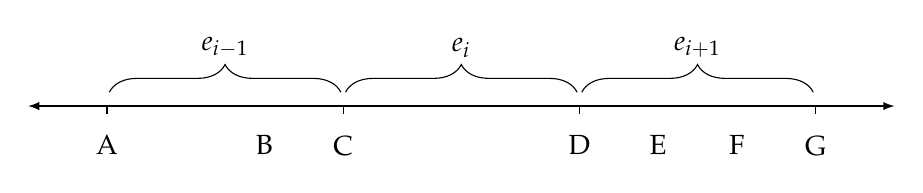
\begin{tikzpicture}
% axis
\draw[latex-latex] (0,0) -- (11,0) ;

% epoch braces
\draw [decorate,decoration={brace,amplitude=10pt} ,yshift=5pt] (1.03,0) -- (3.97,0)
  node [midway, above, yshift=9pt]{$e_{i-1}$};
\draw [decorate,decoration={brace,amplitude=10pt} ,yshift=5pt] (4.03,0) -- (6.97,0)
  node [midway, above, yshift=9pt]{$e_{i}$};
\draw [decorate,decoration={brace,amplitude=10pt} ,yshift=5pt] (7.03,0) -- (9.97,0)
  node [midway, above, yshift=9pt]{$e_{i+1}$};

% epoch boundaries
\foreach \x in  {1,4,7,10}
  \draw[shift={(\x,0)}] (0pt,0pt) -- (0pt,-3pt);

\node at (1,-0.5) {A};
\node at (3,-0.5) {B};
\node at (4,-0.5) {C};
\node at (7,-0.5) {D};
\node at (8,-0.5) {E};
\node at (9,-0.5) {F};
\node at (10,-0.5) {G};

\end{tikzpicture}

We must therefore store the last three stake distributions.
The mnemonic ``mark, set, go'' will be used to keep
track of the snapshots, where the label ``mark'' refers to the most recent snapshot,
and ``go'' refers to the snapshot that is ready to be used in the reward calculation.
In the above diagram, the snapshot taken at (A) is labeled ``mark'' during epoch $e_{i-1}$,
``set'' during epoch $e_i$ and ``go'' during epoch $e_{i+1}$. At (G) the snapshot
taken at (A) is no longer needed and will be discarded.

The two main transition systems in this section are:
\begin{itemize}
  \item The transition system named $\mathsf{EPOCH}$, which is defined in
    Section~\ref{sec:total-epoch}, covers what happens at the epoch boundary,
    such as at (A), (C), (D) and (G).
  \item The transition named $\mathsf{RUPD}$, which is defined in
    Section~\ref{sec:reward-update-trans}, covers the reward calculation that
    happens between (E) and (F).
\end{itemize}


\begin{note}
  Between time D and E we are concerned with chain growth and stability.
  Therefore this duration can be stated as 2k blocks (to state it in slots requires details about
  the particular version of the Ouroboros protocol). The duration between F and G is also 2k blocks.
  Between E and F a single honest block is enough to ensure a random nonce.
\end{note}

\subsection{Example Illustration of the Reward Cycle}
\label{sec:illustration-reward-cycle}

\definecolor{epochColor}{rgb} {1.00,0.50,0.00}
\definecolor{aliceColor}{rgb} {0.65,0.00,0.00}
\definecolor{bobColor}{rgb} {0.00,0.50,0.00}
\definecolor{bob2Color}{rgb} {0.00,0.95,0.00}
\definecolor{snapshot1}{rgb} {0.00,0.00,0.90}
\definecolor{snapshot2}{rgb} {0.00,0.60,0.90}

\begin{tikzpicture}

  % Axis
  \draw [thick] (-0.2,0) -- (13,0);
  \draw (0,-.2) -- (0, .2);
  \draw (3,-.2) -- (3, .2);
  \draw (6,-.2) -- (6, .2);
  \draw (9,-.2) -- (9, .2);
  \draw (12,-.2) -- (12, .2);
  \node[align=center, below, color=epochColor] at (1.5,0.5)
    {$e_1$};
  \node[align=center, below, color=epochColor] at (4.5,0.5)
    {$e_2$};
  \node[align=center, below, color=epochColor] at (7.5,0.5)
    {$e_3$};
  \node[align=center, below, color=epochColor] at (10.5,0.5)
    {$e_4$};

  % Alice
  % Alice's circle
  \draw [aliceColor, fill] (0,3) circle [radius=0.5];
  \node [white] at (0,3) {Alice};
  % Alice's delegation line
  \draw [->,thick, aliceColor] (0.4,2.65) to (2,0.05);
  \node [aliceColor] at (2.2,2) {delegate to Bob};

  % Bob
  % Bob's circle
  \draw [bobColor, fill] (0,-3) circle [radius=0.5];
  \node [white] at (0,-3) {Bob};
  % Bob's registration line
  \draw [->,thick, bobColor] (0.2,-2.50) to (1,-0.05);
  \node [align=left, below, bobColor] at (-0.5,-0.5) {initial pool \\ registration};
  % Bob's re-registration line
  \draw [->,thick, bob2Color] (0.45,-2.65) to (2.90,-0.05);
  \node [bob2Color] at (2,-2.8) {re-registration};
  % Bob's cached parameter change
  \draw [->,thick, bob2Color] (2.9,-0.2) to [out=280, in=180] (3,-2)
     to [out=0, in=290] (3.1,-0.2);

  % Alice time to re-delegate
  \draw [decorate, decoration = {brace, mirror, amplitude=10pt}, aliceColor, thick]
    (3.2,-0.2) to (5.9,-0.2);
  \node [align=center, below, aliceColor] at (5.1,-0.5)
    {Alice's opportunity \\ to re-delegate \\ before Bob's new \\ parameters};

  % Bob's blocks
  % epoch e3
  \draw [fill=bobColor,bobColor] (6.3,-.1) rectangle (6.5,-.3);
  \draw [fill=bobColor,bobColor] (6.7,-.1) rectangle (6.9,-.3);
  \draw [fill=bobColor,bobColor] (7.4,-.1) rectangle (7.6,-.3);
  \draw [fill=bobColor,bobColor] (8.4,-.1) rectangle (8.6,-.3);
  \draw [decorate, decoration = {brace, mirror, amplitude=10pt}, bobColor, thick]
    (6.2, -0.4) to (8.9,-0.4);
  \draw [->,thick, bobColor] (7.6, -0.8) to [out=315,in=200] (8.4, -1.2)
     to [] (9.6, -0.9);

  % epoch e4
  \draw [fill=bob2Color,bob2Color] (9.9,-.1) rectangle (10.1,-.3);
  \draw [fill=bob2Color,bob2Color] (10.4,-.1) rectangle (10.6,-.3);
  \draw [fill=bob2Color,bob2Color] (10.8,-.1) rectangle (11.0,-.3);
  \draw [decorate, decoration = {brace, mirror, amplitude=10pt}, bob2Color, thick]
    (9.7, -0.4) to (11.2,-0.4);
  \draw [->,thick, bob2Color] (10.6, -0.8) to [out=315,in=200] (11.4, -1.2)
     to [] (12.6, -0.9);

  % Snapshots
  \draw [->,thick, snapshot1] (3,0.3) to [out=90,in=150] (9,0.5)
     to [out=330,in=180] (10,-1) to [out=0,in=-135] (12,0) ;
   \node [snapshot1] at (2.7,1.2) {mark};
   \node [snapshot1] at (6,1.9) {set};
   \node [snapshot1] at (9,0.9) {go};

  \draw [->,thick, snapshot2] (6,0.3) to [out=90,in=150] (12,0.5)
     to [out=330,in=180] (13,-1);
   \node [snapshot2] at (5.7,1.2) {mark};
   \node [snapshot2] at (9,1.9) {set};
   \node [snapshot2] at (12,0.9) {go};
\end{tikzpicture}

Bob registers his stake pool in epoch $e_1$.
Alice delegates to Bob's stake pool in epoch $e_1$.
Just before the end of epoch $e_1$, Bob submits a stake pool re-registration,
changing his pool parameters. The change in parameters is not immediate,
as shown by the curved arrow around the epoch boundary.

A snapshot is taken on the $e_1$/$e_2$ boundary. It is labeled ``mark'' initially.
This snapshot includes Alice's delegation to Bob's pool, and Bob's pool parameters
and listed in the initial pool registration certificate.

If Alice changes her delegation choice any time during epoch $e_2$,
she will never be effected by Bob's change of parameters.

A new snapshot is taken on the $e_2$/$e_3$ boundary.
The previous (darker blue) snapshot is now labeled ``set'', and the new one labeled ``mark''.
The ``set'' snapshot is used for leader election in epoch $e_3$.

On the $e_3$/$e_4$ boundary, the darker blue snapshot is labeled ``go'' and
the lighter blue snapshot is labeled ``set''.
Bob's stake pool performance during epoch $e_3$ (he produced 4 blocks)
will be used with the darker blue snapshot for the rewards which will
be handed out at the beginning of epoch $e_5$.

\subsection{Helper Functions and Accounting Fields}
\label{sec:stake-dist-helpers}

Figure~\ref{fig:funcs:epoch-helper-rewards} defines four helper functions needed
throughout the rest of the section.

\begin{itemize}
  \item The function $\fun{obligation}$ calculates the the minimal amount of coin needed to
    pay out all deposit refunds.
  \item The function $\fun{poolStake}$ filters the stake distribution to one stake pool.
\end{itemize}


%%
%% Figure - Helper Functions for Epoch Rules
%%
\begin{figure}[htb]
  \emph{Total possible refunds}
  \begin{align*}
    & \fun{obligation} \in \PParams \to (\StakeCredential \mapsto \Coin)
    \to (\KeyHash_{pool}\mapsto\PoolParam) \to \Coin \\
    & \obligation{pp}{rewards}{poolParams} = \\
    & ~~~~~
    (\fun{keyDeposit}~\var{pp}) \cdot|\var{rewards}| +
    (\fun{poolDeposit}~\var{pp}) \cdot|\var{poolParams}| \\
  \end{align*}
  %
  \emph{Filter Stake to one Pool}
  \begin{align*}
      & \fun{poolStake} \in \KeyHash_{pool} \to (\KeyHash_{stake} \mapsto \KeyHash_{pool})
        \to \Stake \to \Stake \\
      & \poolStake{hk}{delegs}{stake} =
        \dom{(\var{delegs}\restrictrange\{hk\})\restrictdom\var{stake}}
  \end{align*}

  \caption{Helper Functions used in Rewards and Epoch Boundary}
  \label{fig:funcs:epoch-helper-rewards}
\end{figure}


The Figure~\ref{fig:defs:accounting} lists the accounting fields, denoted by $\Acnt$,
which will be used throughout this section. It consists of:
\begin{itemize}
  \item The value $\var{treasury}$ tracks the amount of coin currently stored in the treasury.
    Initially there will be no way to remove these funds.
  \item The value $\var{reserves}$ tracks the amount of coin currently stored in the reserves.
    This pot is used to pay rewards.
\end{itemize}
More will be said about the general accounting system in Section~\ref{sec:reward-calc}.

%%
%% Figure - Accounting fields
%%
\begin{figure}[htb]
  \emph{Accounting Fields}
  \begin{equation*}
    \Acnt =
    \left(
      \begin{array}{r@{~\in~}ll}
        \var{treasury} & \Coin & \text{treasury pot}\\
        \var{reserves} & \Coin & \text{reserve pot}\\
      \end{array}
    \right)
  \end{equation*}
  %
  \caption{Accounting fields}
  \label{fig:defs:accounting}
\end{figure}


\subsection{Stake Distribution Calculation}
\label{sec:stake-dist-calc}

This section defines the stake distribution calculations.
Figure~\ref{fig:epoch-defs} introduces three new derived types:
\begin{itemize}
  \item $\type{BlocksMade}$ represents the number of blocks each stake pool produced
    during an epoch.
  \item $\type{Stake}$ represents the amount of stake (in $\type{Coin}$) controlled by each
    stake pool.
\end{itemize}

%%
%% Figure - Epoch Abstract Types
%%
\begin{figure}[htb]
  \emph{Derived types}
  %
  \begin{equation*}
    \begin{array}{r@{~\in~}l@{\qquad=\qquad}lr}
      \var{blocks}
      & \BlocksMade
      & \KeyHash_{pool} \mapsto \N
      & \text{blocks made by stake pools} \\
      \var{stake}
      & \Stake
      & \Credential \mapsto \Coin
      & \text{stake} \\
    \end{array}
  \end{equation*}
  \caption{Epoch definitions}
  \label{fig:epoch-defs}
\end{figure}

The stake distribution calculation is given in Figure~\ref{fig:functions:stake-distribution}.

\begin{itemize}
\item $\fun{aggregate_{+}}$ takes a relation on $A\times B$, where $B$ is any
  monoid $(B,+,e)$ and returns a map from each $a\in A$ to the ``sum'' (using
  the monoidal $+$ operation) of all $b\in B$ such that $(a, b)\in A\times B$.
\item $\fun{stakeDistr}$ uses the $\fun{aggregate_{+}}$ function and several relations to
    compute the stake distribution, mapping each hashkey to the total coin under its control.
    Keys that are not both registered and delegated are filtered out.
    The relation passed to $\fun{aggregate_{+}}$ is made up of:
    \begin{itemize}
      \item $\fun{stakeCred_b}^{-1}$, relating credentials to (base) addresses
      \item $\left(\fun{addrPtr}\circ\var{ptr}\right)^{-1}$, relating credentials to (pointer)
        addresses
      \item $\range{utxo}$, relating addresses to coins
      \item $\fun{stakeCred_r}^{-1}\circ\var{rewards}$, relating (reward) addresses to coins
    \end{itemize}
    The notation for relations is explained in Section~\ref{sec:notation-shelley}.
\end{itemize}

%%
%% Figure Functions for Stake Distribution
%%
\begin{figure}[htb]
  \emph{Aggregation (for a monoid B)}
  %
  \begin{align*}
      & \fun{aggregate_{+}} \in \powerset{(A \times B)} \to (A\mapsto B) \\
      & \fun{aggregate_{+}}~\var{R} = \left\{a\mapsto \sum_{(a,b)\in\var{R}}b
          ~\mid~a\in\dom\var{R}\right\} \\
  \end{align*}
  %
  \emph{Stake Distribution (using functions and maps as relations)}
  %
  \begin{align*}
      & \fun{stakeDistr} \in \UTxO \to \DState \to \PState \to \Snapshot \\
      & \fun{stakeDistr}~{utxo}~{dstate}~{pstate} = \\
      & ~~~~ \big((\dom{\var{activeDelegs}})
      \restrictdom\left(\fun{aggregate_{+}}~\var{stakeRelation}\right),
    ~\var{delegations},~\var{poolParams}\big)\\
      & \where \\
      & ~~~~ (~\var{rewards},~\var{delegations},~\var{ptrs},~\wcard,~\wcard,~\wcard)
        = \var{dstate} \\
      & ~~~~ (~\var{poolParams},~\wcard,~\wcard) = \var{pstate} \\
      & ~~~~ \var{stakeRelation} = \left(
        \left(\fun{stakeCred_b}^{-1}\cup\left(\fun{addrPtr}\circ\var{ptr}\right)^{-1}\right)
        \circ\left(\range{\var{utxo}}\right)
        \right)
        \cup \var{rewards} \\
      & ~~~~ \var{activeDelegs} =
               (\dom{rewards}) \restrictdom \var{delegations} \restrictrange (\dom{poolParams}) \\
  \end{align*}

  \caption{Stake Distribution Function}
  \label{fig:functions:stake-distribution}
\end{figure}

\clearpage

\subsection{Snapshot Transition}
\label{sec:snapshots}

The state transition types for stake distribution snapshots are given in
Figure~\ref{fig:ts-types:snapshot}.
Each snapshot consists of:
\begin{itemize}
  \item $\var{stake}$, a stake distribution, which is defined in
    Figure~\ref{fig:epoch-defs} as a mapping of credentials to coin.
  \item $\var{delegations}$, a delegation map, mapping credentials to stake pools.
  \item $\var{poolParameters}$, storing the pool parameters of each stake pool.
\end{itemize}

The type $\type{\Snapshots}$ contains the
information needing to be saved on the epoch boundary:
\begin{itemize}
  \item $\var{pstake_{mark}}$, $\var{pstake_{set}}$ and $\var{pstake_{go}}$ are the three
    snapshots as explained in Section~\ref{sec:reward-overview}.
  \item $\var{feeSS}$ stores the fees which are added to the reward pot during
    the next reward update calculation, which is then subtracted from the fee pot
    on the epoch boundary.
\end{itemize}

%%
%% Figure - Snapshots Defs
%%
\begin{figure}[htb]
  \emph{Snapshots}
  \begin{equation*}
    \Snapshot =
    \left(
      \begin{array}{r@{~\in~}ll}
        \var{stake} & \Stake & \text{stake distribution}\\
        \var{delegations} & \Credential\mapsto\KeyHash_{pool}
                          & \text{stake delegations}\\
        \var{poolParameters} & \KeyHash_{pool} \mapsto \PoolParam & \text{pool parameters }\\
      \end{array}
    \right)
  \end{equation*}

  \begin{equation*}
    \Snapshots =
    \left(
      \begin{array}{r@{~\in~}ll}
        \var{pstake_{mark}} & \Snapshot & \text{newest stake}\\
        \var{pstake_{set}}  & \Snapshot & \text{middle stake}\\
        \var{pstake_{go}}   & \Snapshot & \text{oldest stake}\\
        \var{feeSS} & \Coin & \text{fee snapshot}\\
      \end{array}
    \right)
  \end{equation*}
  %
  \emph{Snapshot transitions}
  \begin{equation*}
    \_ \vdash
    \var{\_} \trans{snap}{} \var{\_}
    \subseteq \powerset (\LState \times \Snapshots \times \Snapshots)
  \end{equation*}
  %
  \caption{Snapshot transition-system types}
  \label{fig:ts-types:snapshot}
\end{figure}

The snapshot transition rule is given in Figure~\ref{fig:rules:snapshot}.
This transition has no preconditions and results in the following state change:

\begin{itemize}
  \item The oldest snapshot is replaced with the penultimate one.
  \item The penultimate snapshot is replaced with the newest one.
  \item The newest snapshot is replaced with one just calculated.
  \item The current fees pot is stored in $\var{feeSS}$. Note that this value will not
    change during the epoch, unlike the $\var{fees}$ value in the UTxO state.
\end{itemize}

%%
%% Figure - Snapshot Rule
%%
\begin{figure}[htb]
  \begin{equation}\label{eq:snapshot}
    \inference[Snapshot]
    {
      {
      \begin{array}{r@{~\leteq~}l}
        ((\var{utxo},~\wcard,\var{fees},~\wcard),~(\var{dstate},~\var{pstate})) & \var{lstate} \\
        \var{stake} & \stakeDistr{utxo}{dstate}{pstate} \\
      \end{array}
      }
    }
    {
      \begin{array}{r}
        \var{lstate} \\
      \end{array}
      \vdash
      \left(
        \begin{array}{r}
          \var{pstake_{mark}}\\
          \var{pstake_{set}}\\
          \var{pstake_{go}}\\
          \var{feeSS} \\
        \end{array}
      \right)
      \trans{snap}{}
      \left(
        \begin{array}{r}
          \varUpdate{\var{stake}} \\
          \varUpdate{\var{pstake_{mark}}} \\
          \varUpdate{\var{pstake_{set}}} \\
          \varUpdate{\var{fees}} \\
        \end{array}
      \right)
    }
  \end{equation}
  \caption{Snapshot Inference Rule}
  \label{fig:rules:snapshot}
\end{figure}

\clearpage

\subsection{Pool Reaping Transition}
\label{sec:pool-reap}

Figure~\ref{fig:ts-types:pool-reap} defines the types for the pool reap transition,
which is responsible for removing pools slated for retirement in the given epoch.

%%
%% Figure - Pool Reap Defs
%%
\begin{figure}[htb]
  \emph{Pool Reap State}
  \begin{equation*}
    \PlReapState =
    \left(
      \begin{array}{r@{~\in~}ll}
        \var{utxoSt} & \UTxOState & \text{utxo state}\\
        \var{acnt} & \Acnt & \text{accounting}\\
        \var{dstate} & \DState & \text{delegation state}\\
        \var{pstate} & \PState & \text{pool state}\\
      \end{array}
    \right)
  \end{equation*}
  %
  \emph{Pool Reap transitions}
  \begin{equation*}
    \_ \vdash \_ \trans{poolreap}{\_} \_ \in
    \powerset (\PParams \times \PlReapState \times \Epoch \times \PlReapState)
  \end{equation*}
  %
  \caption{Pool Reap Transition}
  \label{fig:ts-types:pool-reap}
\end{figure}


The pool-reap transition rule is given in Figure~\ref{fig:rules:pool-reap}.
This transition has no preconditions and results in the following state change:

\begin{itemize}
  \item For each retiring pool, the refund for the pool registration deposit is added to the
    pool's registered reward account, provided the reward account is still registered.
  \item The sum of all the refunds attached to unregistered reward accounts are added to the
    treasury.
  \item The deposit pool is reduced by the amount of claimed and unclaimed refunds.
  \item Any delegation to a retiring pool is removed.
  \item Each retiring pool is removed from all four maps in the pool state.
\end{itemize}

%%
%% Figure - Pool Reap Rule
%%
\begin{figure}[htb]
  \begin{equation}\label{eq:pool-reap}
    \inference[Pool-Reap]
    {
      {
      \begin{array}{r@{~\leteq~}l}
        \var{retired} & \dom{(\var{retiring}^{-1}~\var{e})} \\
        \var{pr} & \left\{
                   \var{hk}\mapsto(\fun{poolDeposit}~\var{pp})
                     \mid
                     \var{hk}\in\var{retired}
                   \right\}\\
        \var{rewardAcnts}
                 & \{\var{hk}\mapsto \fun{poolRAcnt}~\var{pool} \mid
                   \var{hk}\mapsto\var{pool} \in \var{retired}\restrictdom\var{poolParams} \} \\
        \var{rewardAcnts'} & \left\{
                               a \mapsto
                               \sum\var{pr}(\var{rewardAcnts}^{-1}(a))
                               \mathrel{\Big|}
                               a\in\range{rewardAcnts}
                             \right\} \\
        \var{refunds} & \dom{rewards}\restrictdom\var{rewardAcnts'} \\
        \var{mRefunds} & \dom{rewards}\subtractdom\var{rewardAcnts'} \\
        \var{refunded} & \sum\limits_{\wcard\mapsto c\in\var{refunds}} c \\
        \var{unclaimed} & \sum\limits_{\wcard\mapsto c\in\var{mRefunds}} c \\
      \end{array}
      }
    }
    {
      \var{pp}
      \vdash
      \left(
        \begin{array}{r}
          \var{utxo} \\
          \var{deposited} \\
          \var{fees} \\
          \var{ppup} \\
          ~ \\
          \var{treasury} \\
          \var{reserves} \\
          ~ \\
          \var{rewards} \\
          \var{delegations} \\
          \var{ptrs} \\
          \var{genDelegs} \\
          \var{fGenDelegs} \\
          \var{i_{rwd}} \\
          ~ \\
          \var{poolParams} \\
          \var{fPoolParams} \\
          \var{retiring} \\
        \end{array}
      \right)
      \trans{poolreap}{e}
      \left(
        \begin{array}{rcl}
          \var{utxo} \\
          \varUpdate{\var{deposited}}
          & \varUpdate{-}
          & \varUpdate{(\var{unclaimed} + \var{refunded})} \\
          \var{fees} \\
          \var{ppup} \\
          ~ \\
          \varUpdate{\var{treasury}} & \varUpdate{+} & \varUpdate{\var{unclaimed}} \\
          \var{reserves} \\
          ~ \\
          \varUpdate{\var{rewards}} & \varUpdate{\unionoverridePlus} & \varUpdate{\var{refunds}} \\
          \varUpdate{\var{delegations}} & \varUpdate{\subtractrange} & \varUpdate{\var{retired}} \\
          \var{ptrs} \\
          \var{genDelegs} \\
          \var{fGenDelegs} \\
          \var{i_{rwd}}\\
          ~ \\
          \varUpdate{\var{retired}} & \varUpdate{\subtractdom} & \varUpdate{\var{poolParams}} \\
          \varUpdate{\var{retired}} & \varUpdate{\subtractdom} & \varUpdate{\var{fPoolParams}} \\
          \varUpdate{\var{retired}} & \varUpdate{\subtractdom} & \varUpdate{\var{retiring}} \\
        \end{array}
      \right)
    }
  \end{equation}
  \caption{Pool Reap Inference Rule}
  \label{fig:rules:pool-reap}
\end{figure}

\clearpage

\subsection{Protocol Parameters Update Transition}
\label{sec:pparam-update}

Finally, reaching the epoch boundary may trigger a change in the protocol parameters.
The protocol parameters environment consists of the delegation and pool states,
and the signal is an optional new collection of protocol parameters
The state change is a change of the $\UTxOState$, the $\Acnt$ states and the current $\PParams$.
The type of this state transition is given in Figure~\ref{fig:ts-types:new-proto-param}.

%%
%% Figure - New Proto Param Defs
%%
\begin{figure}[htb]
  \emph{New Proto Param environment}
  \begin{equation*}
    \NewPParamEnv =
    \left(
      \begin{array}{r@{~\in~}ll}
        \var{dstate} & \DState & \text{delegation state}\\
        \var{pstate} & \PState & \text{pool state}\\
      \end{array}
    \right)
  \end{equation*}
  %
  \emph{New Proto Param States}
  \begin{equation*}
    \NewPParamState =
    \left(
      \begin{array}{r@{~\in~}ll}
        \var{utxoSt} & \UTxOState & \text{utxo state}\\
        \var{acnt} & \Acnt & \text{accounting}\\
        \var{pp} & \PParams & \text{current protocol parameters}\\
      \end{array}
    \right)
  \end{equation*}
  %
  \emph{New Proto Param transitions}
  \begin{equation*}
    \_ \vdash
    \var{\_} \trans{newpp}{\_} \var{\_}
    \subseteq \powerset (\NewPParamEnv \times \NewPParamState \times \PParams^? \times \NewPParamState)
  \end{equation*}
  %
  \caption{New Proto Param transition-system types}
  \label{fig:ts-types:new-proto-param}
  %
  \emph{Helper Functions}
  \begin{align*}
      & \fun{updatePpup} \in \UTxOState \to \PParams \to \UTxOState\\
      & \fun{updatePpup}~\var{utxoSt}~\var{pp} =
      \begin{cases}
        (\var{utxo},\var{deposited},\var{fees},(\var{fpup},~\emptyset))
        &
        \var{canFollow}
        \\
        (\var{utxo},\var{deposited},\var{fees},(\emptyset,~\emptyset))
        &
        \text{otherwise} \\
      \end{cases}\\
      & ~~~\where \\
      & ~~~~~~~\var{canFollow} =
        \forall\var{ps}\in\range{pup},~
        \var{pv}\mapsto\var{v}\in\var{ps}\implies\fun{pvCanFollow}~(\fun{pv}~\var{pp})~\var{v}
        \\
      & ~~~~~~~(\var{utxo},\var{deposited},\var{fees},(\var{pup},~\var{fpup})) = \var{utxoSt} \\
  \end{align*}
\end{figure}


Figure~\ref{fig:rules:new-proto-param} defines the new protocol parameter transition.
The transition has two rules, depending on whether or not the new protocol parameters
meet some requirements.
In particular, we require that the new parameters would not incur a debt of the system that
can not be covered by the reserves, and that the max block size is greater than the sum of the
max transaction size and the max header size.
If the requirements are met, the new protocol parameters are accepted, the proposal is reset,
and the reserves are adjusted to account for changes in the deposits.
Otherwise, the only change is that the proposal is reset.

The $\mathsf{NEWPP}$ rule also cleans up the protocol parameter update proposals,
by calling $\fun{updatePpup}$ on the UTxO state.
The $\fun{updatePpup}$ sets the protocol parameter updates to the future protocol
parameter updates provided the protocol versions all can follow from the
version given in the protocol parameters, or the emptyset otherwise.
In any case, the future protocol parameters update proposals are set to the empty set.
If new protocol parameters are being adopted, then these is the value given to
$\fun{updatePpup}$, otherwise the old parameters are given.

Regarding adjusting the reserves for changes in the deposits, one of three things happens:

\begin{itemize}
  \item If the new protocol parameters mean that \textbf{fewer} funds are required in the
    deposit pot to cover all possible refunds, then the excess is moved to the reserves.

  \item If the new protocol parameters mean that \textbf{more} funds are required in the
    deposit pot to cover all possible refunds and the difference is \textbf{less} than
    the reserve pot, then funds are moved from the reserve pot to cover the difference.

  \item If the new protocol parameters mean that \textbf{more} funds are required in the
    deposit pot to cover all possible refunds and the difference is \textbf{more} than
    the reserve pot, then Rule~\ref{eq:new-pc-denied} meets the precondition and the
    only change of state is that the update proposals are reset.
\end{itemize}

Note that here, unlike most of the inference rules in this document,
the $\var{utxoSt'}$ and the $\var{acnt'}$ do not come from valid UTxO or
accounts transitions in the antecedent. We simply define the consequent
transition using these directly (instead of listing all the fields in both
states in the consequent transition). It is done this way here
for ease of reading.

%%
%% Figure - New Proto Param Rule
%%
\begin{figure}[htb]
  \begin{equation}\label{eq:new-pc-accepted}
    \hspace{-0.3cm}
    \inference[New-Proto-Param-Accept]
    {
      \var{pp_{new}}\neq\Nothing \\~\\
      {\begin{array}{rcl}
         (\var{utxo},~\var{deposited},~\var{fees},~\var{ppup}) & \leteq & \var{utxoSt} \\
         \var{(\var{rewards},~\wcard,~\wcard,~\wcard,~\wcard,~\var{i_{rwd}})} &
         \leteq & \var{dstate}\\
         \var{(\var{poolParams},~\wcard,~\wcard)} & \leteq & \var{pstate}\\
         \var{oblg_{cur}} & \leteq & \obligation{pp}{rewards}{poolParams} \\
         \var{oblg_{new}} & \leteq & \obligation{pp_{new}}{rewards}{poolParams} \\
         \var{diff} & \leteq & \var{oblg_{cur}} - \var{oblg_{new}}\\
      \end{array}}
      \\~\\~\\
      \var{oblg_{cur}} = \var{deposited} \\
      \var{reserves} + \var{diff} \geq \sum\limits_{\wcard\mapsto\var{val}\in\var{i_{rwd}}} val \\
      \fun{maxTxSize}~\var{pp_{new}} + \fun{maxHeaderSize}~\var{pp_{new}} <
        \fun{maxBlockSize}~\var{pp_{new}}
      \\~\\
        \var{utxoSt'} \leteq
        \left(\var{utxo},~\varUpdate{oblg_{new}},~\var{fees},~\var{ppup}\right)
      \\
      \var{utxoSt''} \leteq \fun{updatePpup}~\var{utxoSt'}~\var{pp_{new}}
      \\~\\
      (\var{treasury},~\var{reserves})\leteq \var{acnt} \\
      \var{acnt'} \leteq (\var{treasury},~\varUpdate{reserves + diff}) \\
    }
    {
      \begin{array}{l}
        \var{dstate}\\
        \var{pstate}\\
      \end{array}
      \vdash
      \left(
        \begin{array}{r}
          \var{utxoSt} \\
          \var{acnt} \\
          \var{pp}
        \end{array}
      \right)
      \trans{newpp}{\var{pp_{new}}}
      \left(
        \begin{array}{rcl}
          \varUpdate{utxoSt''}\\
          \varUpdate{acnt'} \\
          \varUpdate{\var{pp_{new}}} \\
        \end{array}
      \right)
    }
  \end{equation}

  \nextdef

  \begin{equation}\label{eq:new-pc-denied}
    \inference[New-Proto-Param-Denied]
    {
      \left({\begin{array}{c}
            \var{pp_{new}}=\Nothing \\
        \lor \\
        \var{reserves} + \var{diff} < \sum\limits_{\wcard\mapsto\var{val}\in\var{i_{rwd}}} val\\
        \lor \\
        \fun{maxTxSize}~\var{pp_{new}} + \fun{maxHeaderSize}~\var{pp_{new}} \geq
          \fun{maxBlockSize}~\var{pp_{new}}
      \end{array}}\right)
      \\~\\~\\
      {\begin{array}{rcl}
          \var{(\var{rewards},~\wcard,~\wcard,~\wcard,~\wcard,~\var{i_{rwd}})} &
          \leteq & \var{dstate}\\
         \var{(\var{poolParams},~\wcard,~\wcard)} & \leteq & \var{pstate}\\
          \var{oblg_{cur}} & \leteq & \obligation{pp}{rewards}{poolParams} \\
          \var{oblg_{new}} & \leteq & \obligation{pp_{new}}{rewards}{poolParams} \\
         \var{diff} & \leteq & \var{oblg_{cur}} - \var{oblg_{new}}
      \end{array}}
      \\~\\~\\
      \var{utxoSt'} \leteq \fun{updatePpup}~\var{utxoSt}~\var{pp} \\
    }
    {
      \begin{array}{l}
        \var{dstate}\\
        \var{pstate}\\
      \end{array}
      \vdash
      \left(
        \begin{array}{r}
          \var{utxoSt} \\
          \var{acnt} \\
          \var{pp}
        \end{array}
      \right)
      \trans{newpp}{\var{pp_{new}}}
      \left(
        \begin{array}{rcl}
          \varUpdate{utxoSt'}\\
          \var{acnt} \\
          \var{pp}
        \end{array}
      \right)
    }
  \end{equation}
  \caption{New Proto Param Inference Rule}
  \label{fig:rules:new-proto-param}
\end{figure}

\clearpage

\subsection{Complete Epoch Boundary Transition}
\label{sec:total-epoch}

Finally, it is possible to define the complete epoch boundary transition type,
which is defined in Figure~\ref{fig:ts-types:epoch}.
The transition has no evironment.
The state is made up of the the accounting state, the snapshots, the ledger state and the
protocol parameters.
The transition uses a helper function $\fun{votedValue}$ which returns
the consensus value of update proposals in the event that consensus is met.
\textbf{Note that} $\fun{votedValue}$
\textbf{is only well-defined if } $\var{quorum}$
\textbf{is greater than half the number of core nodes, i.e.}
$\Quorum > |\var{genDelegs}|/2$ \textbf{.}

%%
%% Figure - Epoch Defs
%%
\begin{figure}[htb]
  \emph{Epoch States}
  \begin{equation*}
    \EpochState =
    \left(
      \begin{array}{r@{~\in~}ll}
        \var{acnt} & \Acnt & \text{accounting}\\
        \var{ss} & \Snapshots & \text{snapshots}\\
        \var{ls} & \LState & \text{ledger state}\\
        \var{prevPp} & \PParams & \text{previous protocol parameters}\\
        \var{pp} & \PParams & \text{protocol parameters}\\
      \end{array}
    \right)
  \end{equation*}
  %
  \emph{Epoch transitions}
  \begin{equation*}
    \vdash
    \var{\_} \trans{epoch}{\_} \var{\_}
    \subseteq \powerset (\EpochState \times \Epoch \times \EpochState)
  \end{equation*}
  %
  \emph{Accessor Functions}
  \begin{equation*}
    \begin{array}{r@{~\in~}lr}
      \fun{getIR} & \EpochState \to (\StakeCredential \mapsto \Coin)
                  & \text{get instantaneous rewards} \\
    \end{array}
  \end{equation*}
  %
  \emph{Helper Functions}
  \begin{align*}
      & \fun{votedValue} \in (\KeyHashGen\mapsto\PParamsUpdate) \to \PParams \to \N \to \PParamsUpdate^?\\
      & \fun{votedValue}~\var{pup}~\var{pp}~\var{quorum} =
      \begin{cases}
        \var{pp}\unionoverrideRight\var{p}
          & \exists! p\in\range{pup}~(|pup\restrictrange p|\geq \var{quorum}) \\
        \Nothing & \text{otherwise} \\
      \end{cases}
  \end{align*}
  %
  \caption{Epoch transition-system types}
  \label{fig:ts-types:epoch}
\end{figure}


The epoch transition rule calls $\mathsf{SNAP}$, $\mathsf{POOLREAP}$ and $\mathsf{NEWPP}$
in sequence. It also stores the previous protocol parameters in $\var{prevPp}$.
The previous protocol parameters will be used for the reward calculation in the upcoming epoch,
note that they correspond to the epoch for which the rewards are being calculated.
Additionally, this transition also adopts the pool parameters $\var{fPoolParams}$
corresponding to the pool re-registration certificates which we submitted late in the ending epoch.
The ordering of these rules is important.
The stake pools which will be updated by $\var{fPoolParams}$ or
reaped during the $\mathsf{POOLREAP}$ transition must still be a
part of the new snapshot, and so $\mathsf{SNAP}$ must occur before these two actions.
Moreover, $\mathsf{SNAP}$ sets the deposit pot equal to current obligation,
which is a property that is preserved by $\mathsf{POOLREAP}$ and which
is necessary for the preservation of Ada property in the $ \mathsf{NEWPP}$ transition.

%%
%% Figure - Epoch Rule
%%
\begin{figure}[htb]
  \begin{equation}\label{eq:epoch}
    \inference[Epoch]
    {
      {
        \begin{array}{r}
          \var{lstate} \\
        \end{array}
      }
      \vdash
      { \var{ss} }
      \trans{\hyperref[fig:rules:snapshot]{snap}}{}
      { \var{ss'} }
      \\~\\
      (\var{utxoSt},~(\var{dstate},~\var{pstate}))\leteq\var{ls} \\
      (\var{poolParams},~\var{fPoolParams},~\var{retiring})\leteq\var{pstate}
      \\
      \var{pstate'}\leteq(\var{poolParams}\unionoverrideRight\var{fPoolParams},
      ~\emptyset,~\var{retiring})
      \\~\\~\\
      \var{pp}
      \vdash
      \left(
        {
          \begin{array}{r}
            \var{utxoSt} \\
            \var{acnt} \\
            \var{dstate} \\
            \var{pstate'} \\
          \end{array}
        }
      \right)
      \trans{\hyperref[fig:rules:pool-reap]{poolreap}}{e}
      \left(
      {
        \begin{array}{rcl}
            \var{utxoSt'} \\
            \var{acnt'} \\
            \var{dstate'} \\
            \var{pstate''} \\
        \end{array}
      }
      \right)
      \\~\\~\\
      \var{(\wcard,~\wcard,~\wcard,~(\var{pup},\wcard))}\leteq\var{utxoSt'}\\
      \var{pp_{new}}\leteq\fun{votedValue}~\var{pup}~\var{pp}~\Quorum\\
      {
        \begin{array}{r}
          \var{dstate'}\\
          \var{pstate''}\\
        \end{array}
      }
      \vdash
      \left(
        {
          \begin{array}{r}
            \var{utxoSt'} \\
            \var{acnt'} \\
            \var{pp}\\
          \end{array}
        }
      \right)
      \trans{\hyperref[fig:rules:new-proto-param]{newpp}}{\var{pp_{new}}}
      \left(
      {
        \begin{array}{rcl}
            \var{utxoSt''} \\
            \var{acnt''} \\
            \var{pp'}\\
        \end{array}
      }
      \right)
      \\~\\~\\
      \var{ls}' \leteq (\var{utxoSt}'',~(\var{dstate}',~\var{pstate}''))
    }
    {
      \vdash
      \left(
      \begin{array}{r}
        \var{acnt} \\
        \var{ss} \\
        \var{ls} \\
        \var{prevPp} \\
        \var{pp} \\
      \end{array}
      \right)
      \trans{epoch}{e}
      \left(
      \begin{array}{rcl}
        \varUpdate{\var{acnt''}} \\
        \varUpdate{\var{ss'}} \\
        \varUpdate{\var{ls'}} \\
        \varUpdate{\var{pp}} \\
        \varUpdate{\var{pp'}} \\
      \end{array}
      \right)
    }
  \end{equation}
  \caption{Epoch Inference Rule}
  \label{fig:rules:epoch}
\end{figure}

\clearpage

\subsection{Rewards Distribution Calculation}
\label{sec:reward-dist}

This section defines the reward calculation for the proof of stake leader election.
Figure~\ref{fig:functions:rewards} defines the pool reward as described in section
5.5.2 of~\cite{delegation_design}.

\begin{itemize}
  \item The function $\fun{maxPool}$ gives the maximum reward a stake pool can receive in an epoch.
    This is a fraction of the total available rewards for the epoch.
    The result depends on the pool's relative stake, the pool's pledge and the following
    protocol parameters:
    \begin{itemize}
      \item $\var{a_0}$, the leader-stake influence
      \item $n_{opt}$, the optimal number of saturated stake pools
    \end{itemize}
  \item The function $\fun{mkApparentPerformance}$ computes the apparent performance of a stake pool.
    It depends on the protocol parameter $d$, the relative stake $\sigma$, the number $n$ of blocks
    the pool added to the chain and the total number $\overline{N}$ of blocks added to the chain in
    the last epoch.

\end{itemize}

%%
%% Figure - Functions for the Reward Calculation
%%
\begin{figure}[htb]
  \emph{Maximal Reward Function, called $f(s,\sigma)$ in section 5.5.2 of~\cite{delegation_design}}
  %
  \begin{align*}
      & \fun{maxPool} \in \PParams \to \Coin \to \unitInterval \to \unitInterval \to \Coin \\
      & \fun{maxPool}~\var{pp}~\var{R}~\sigma~\var{p_r} =
          ~~~\floor*{
             \frac{R}{1 + a_0}
             \cdot
             \left(
               \sigma' + p'\cdot a_0\cdot\frac{\sigma' - p'\frac{z_0-\sigma'}{z_0}}{z_0}
             \right)} \\
      & ~~~\where \\
      & ~~~~~~~a_0 = \fun{influence}~pp \\
      & ~~~~~~~n_{opt} = \fun{nopt}~pp \\
      & ~~~~~~~z_0 = 1/n_{opt} \\
      & ~~~~~~~\sigma'=\min(\sigma,~z_0) \\
      & ~~~~~~~p'=\min(p_r,~z_0) \\
  \end{align*}

  \emph{Apparent Performance, called $\hat{p}$ in section 5.5.2 of~\cite{delegation_design}}
  %
  \begin{align*}
      & \fun{mkApparentPerformance} \in \unitInterval \to \unitInterval \to \N \to \N \to \Q \\
      & \mkApparentPerformance{d}{\sigma}{n}{\overline{N}} =
        \begin{cases}
          \frac{\beta}{\sigma} & \text{if } d < 0.8 \\
          1 & \text{otherwise}
        \end{cases} \\
      & ~~~\where \\
      & ~~~~~~~\beta = \frac{n}{\max(1, \overline{N})} \\
  \end{align*}
  \caption{Functions used in the Reward Calculation}
  \label{fig:functions:rewards}
\end{figure}

\clearpage

Figure~\ref{fig:functions:reward-splitting} gives the calculation for
splitting the pool rewards with its members, as described in 6.5.2 of \cite{delegation_design}.
The portion of rewards allocated to the pool operator and owners is different
than that of the members.

\begin{itemize}
  \item The $\fun{r_{operator}}$ function calculates the leader reward, based on the pool cost,
    margin and the proportion of the pool's total stake.  Note that this reward will go to the
    reward account specified in the pool registration certificate.
  \item The $\fun{r_{member}}$ function calculates the member reward, proportionally to their
    stake after the cost and margin are removed.
\end{itemize}

%%
%% Figure - Functions for the Reward Splitting
%%
\begin{figure}[htb]
  \emph{Pool leader reward, from section 5.5.3 of \cite{delegation_design}}
  %
  \begin{align*}
      & \fun{r_{operator}} \in \Coin \to \PoolParam \to \unitInterval \to \unitIntervalNonNull \to \Coin \\
      & \lReward{\hat{f}}{pool}{s}{\sigma} =
        \begin{cases}
        \hat{f} & \hat{f} \leq c\\
        c + \floor*{(\hat{f} - c)\cdot\left(m + (1-m)\cdot\frac{s}{\sigma}\right) }&
        \text{otherwise.}
      \end{cases} \\
      & ~~~\where \\
      & ~~~~~~~c = \fun{poolCost}~pool \\
      & ~~~~~~~m = \fun{poolMargin}~pool \\
  \end{align*}

  \emph{Pool member reward, from section 5.5.3 of \cite{delegation_design}}
  %
  \begin{align*}
    & \fun{r_{member}} \in \Coin \to \PoolParam \to \unitInterval \to \unitIntervalNonNull \to \Coin \\
    & \mReward{\hat{f}}{pool}{t}{\sigma} =
      \begin{cases}
        0 & \hat{f} \leq c\\
        \floor*{(\hat{f} - c)\cdot(1-m)\cdot\frac{t}{\sigma}} &
        \text{otherwise.}
      \end{cases} \\
    & ~~~\where \\
    & ~~~~~~~c = \fun{poolCost}~pool \\
    & ~~~~~~~m = \fun{poolMargin}~pool \\
  \end{align*}

  \caption{Functions used in the Reward Splitting}
  \label{fig:functions:reward-splitting}
\end{figure}


Finally, the full reward calculation is presented in Figure~\ref{fig:functions:reward-calc}.
The calculation is done pool-by-pool.
\begin{itemize}
\item The $\fun{rewardOnePool}$ function calculates the rewards given out to
  each member of a given pool. The pool leader is identified by the stake
  credential of the pool operator. The function returns the rewards, calculated
  as follows:
    \begin{itemize}
      \item $\var{pstake}$, the total amount of stake controlled by the stake pool.
      \item $\var{ostake}$, the total amount of stake controlled by the stake pool operator
        and owners
      \item $\sigma$, the total proportion of stake controlled by the stake pool.
      \item $\overline{N}$, the expected number of blocks the pool should have produced.
      \item $\var{pledge}$, the pool's pledge in lovelace.
      \item $p_r$, the pool's pledge, as a proportion of active stake.
      \item $\var{maxP}$, maximum rewards the pool can claim if the pledge is met,
        and zero otherwise.
      \item $\var{poolR}$, the pool's actual reward, based on its performance.
      \item $\var{mRewards}$, the member's rewards as a mapping of reward accounts to coin.
      \item $\var{lReward}$, the leader's reward as coin.
      \item $\var{potentialRewards}$, the combination of $\var{mRewards}$ and $\var{lRewards}$.
      \item $\var{rewards}$, the restriction of $\var{potentialRewards}$ to the active
        reward accounts.
    \end{itemize}
  \item The $\fun{reward}$ function applies $\fun{rewardOnePool}$ to each registered stake pool.
\end{itemize}

%%
%% Figure - The Reward Calculation
%%
\begin{figure}[htb]
  \emph{Calculation to reward a single stake pool}
  %
  \begin{align*}
    & \fun{rewardOnePool} \in \PParams \to \Coin \to \N \to \N \to \PoolParam\\
      & ~~~\to \Stake \to \Q \to \Q \to \Coin \to \powerset{\AddrRWD}
           \to (\AddrRWD \mapsto \Coin) \\
      & \fun{rewardOnePool}~\var{pp}~\var{R}~\var{n}~\var{\overline{N}}~\var{pool}~\var{stake}~{\sigma}~{\sigma_a}~\var{tot}~\var{addrs_{rew}} =
          \var{rewards}\\
      & ~~~\where \\
      & ~~~~~~~\var{ostake} = \sum_{\substack{
        hk_\mapsto c\in\var{stake}\\
        hk\in(\fun{poolOwners}~\var{pool})\\
        }} c \\
      & ~~~~~~~\var{pledge} = \fun{poolPledge}~pool \\
      & ~~~~~~~p_{r} = \var{pledge} / \var{tot} \\
      & ~~~~~~~maxP =
      \begin{cases}
        \fun{maxPool}~\var{pp}~\var{R}~\sigma~\var{p_r}&
        \var{pledge} \leq \var{ostake}\\
        0 & \text{otherwise.}
      \end{cases} \\
      & ~~~~~~~\var{appPerf} = \mkApparentPerformance{(\fun{d}~pp)}{\sigma_a}{n}{\overline{N}} \\
      & ~~~~~~~\var{poolR} = \floor{\var{appPerf}\cdot\var{maxP}} \\
      & ~~~~~~~\var{mRewards} = \\
      & ~~~~~~~~~~\left\{
                    \addrRw~hk\mapsto\mReward{poolR}{pool}{\frac{c}{tot}}{\sigma}
                    ~\Big\vert~
                    hk\mapsto c\in\var{stake},~~hk \not\in(\fun{poolOwners}~\var{pool})
                  \right\}\\
      & ~~~~~~~\var{lReward} = \lReward{poolR}{pool}{\frac{\var{ostake}}{tot}}{\sigma} \\
      & ~~~~~~~\var{potentialRewards} =
                 \var{mRewards} \cup
                 \{(\fun{poolRAcnt}~\var{pool})\mapsto\var{lReward}\} \\
      & ~~~~~~~\var{rewards} = \var{addrs_{rew}}\restrictdom{\var{potentialRewards}} \\
  \end{align*}

  \emph{Calculation to reward all stake pools}
  %
  \begin{align*}
      & \fun{reward} \in \PParams \to \BlocksMade \to \Coin\to \powerset{\AddrRWD}
      \to (\KeyHash \mapsto \PoolParam) \\
      & ~~~\to \Stake \to (\KeyHash_{stake} \mapsto \KeyHash_{pool}) \to
      \Coin \to (\AddrRWD \mapsto \Coin)\\
      & \reward{pp}{blocks}{R}{addrs_{rew}}{poolParams}{stake}{delegs}{total}
          = \var{rewards}\\
      & ~~~\where \\
      & ~~~~~~~\var{total}_a = \sum_{\_\mapsto c\in \var{stake}}c \\
      & ~~~~~~~\var{\overline{N}} = \sum_{\_\mapsto m\in blocks}m \\
      & ~~~~~~~pdata = \left\{
        hk\mapsto \left(p,~n,~\poolStake{hk}{delegs}{stake}\right)
        \mathrel{\Bigg|}
        \begin{array}{r@{\mapsto}c@{~\in~}l}
          hk & \var{p} & \var{poolParams} \\
          hk & \var{n} & \var{blocks} \\
        \end{array}
      \right\} \\
      & ~~~~~~~\var{results} = \\
      & ~~~~~~~\left\{
        hk \mapsto \fun{rewardOnePool}~
                     \var{pp}~
                     \var{R}~
                     \var{n}~
                     \var{\overline{N}}~
                     \var{p}~
                     \var{s}~
                     \frac{\sum s}{total}~
                     \frac{\sum s}{\var{total}_a}~
                     \var{total}~
                     \var{addrs_{rew}}
                 \mid
        hk\mapsto(p, n, s)\in\var{pdata} \right\} \\
      & ~~~~~~~\var{rewards} = \bigcup_{\wcard\mapsto\var{r}\in\var{results}}\var{r}
  \end{align*}
  \caption{The Reward Calculation}
  \label{fig:functions:reward-calc}
\end{figure}

\clearpage

\subsection{Reward Update Calculation}
\label{sec:reward-calc}

This section defines the calculation of a reward update.
A reward update is the information needed to account for the movement of lovelace
in the system due to paying out rewards.

Figure~\ref{fig:fund-preservation} captures the potential movement of funds in the entire system,
taking every transition system in this document into account.  Value is moved between
accounting pots, but the total amount of value in the system remains constant.
In particular, the red subgraph represents the inputs and outputs to
the ``reward pot'', a temporary variable used during the reward update calculation in
Figure~\ref{fig:functions:reward-update-creation}.
The blue arrows represent the movement of funds that pass through the ``reward pot''.


\begin{figure}[htb]
  \begin{center}
    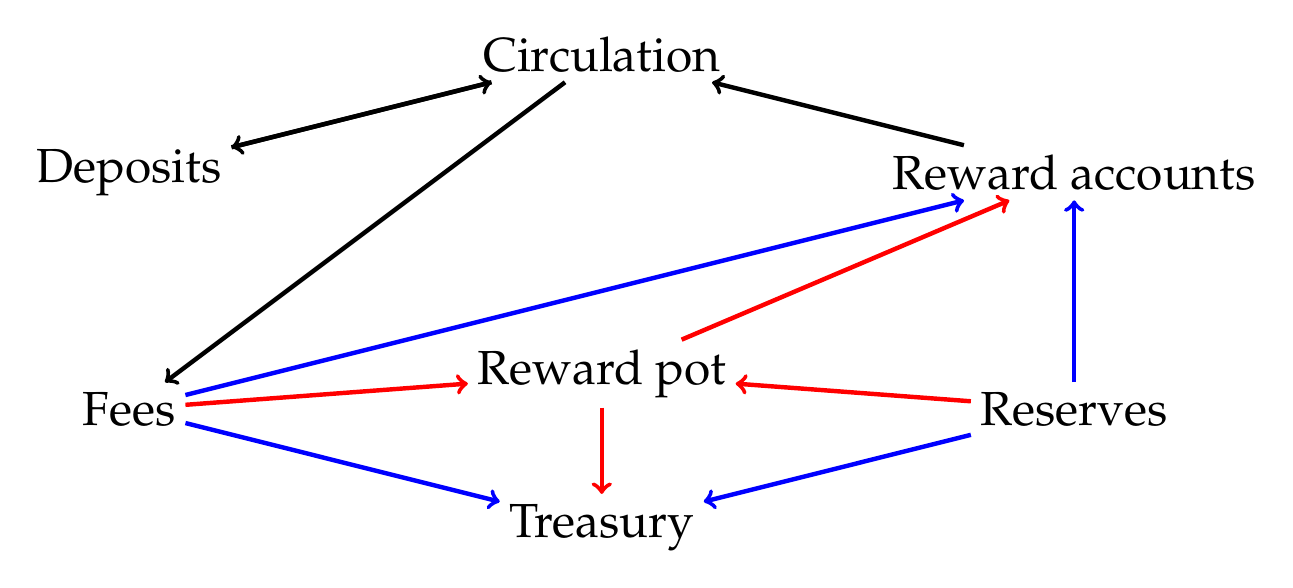
\begin{tikzpicture}
      [ x=30mm, y=30mm
      , direct/.style={black, draw}
      , implied/.style={blue, draw}
      , toTotPot/.style={red, draw}
      ]
    \node (C) at (3,2.5) {\LARGE Circulation};
    \node (R) at (5, 1) {\LARGE Reserves};
    \node (D) at (1, 2) {\LARGE Deposits};
    \node (FR) at (1,1) {\LARGE Fees};
    \node (RA) at (5, 2) {\LARGE Reward accounts};
    \node (T) at (3,0.5) {\LARGE Treasury};

    \draw[->, direct, ultra thick]
    (C) edge (D)
    (C) edge (FR)

    (D) edge (C)

    (RA) edge (C);

    \draw[->, implied, ultra thick]
    (FR) edge (T)
    (FR) edge (RA)

    (R) edge (T)
    (R) edge (RA);

    \node (TP) at (3, 1.15) {\LARGE Reward pot};

    \draw[->, toTotPot, ultra thick]
    (FR) edge (TP)
    (R) edge (TP)

    (TP) edge (RA)
    (TP) edge (T);
    \end{tikzpicture}
  \end{center}
  \caption{Preservation of Value}
  \label{fig:fund-preservation}
\end{figure}

Figure~\ref{fig:defs:reward-update} defines a reward update.
It consists of four pots:
\begin{itemize}
  \item The change to the treasury. This will be a positive value.
  \item The change to the reserves. This will be a negative value.
  \item The map of new individual rewards (to be added to the existing rewards).
  \item The change to the fee pot. This will be a negative value.
    rewards.
\end{itemize}

%%
%% Figure - Reward Update Defs
%%
\begin{figure}[htb]
  \emph{Reward Update}
  \begin{equation*}
    \RewardUpdate =
    \left(
      \begin{array}{r@{~\in~}ll}
        \Delta t & \Coin & \text{change to the treasury} \\
        \Delta r & \Coin & \text{change to the reserves} \\
        \var{rs} & \AddrRWD\mapsto\Coin & \text{new individual rewards} \\
        \Delta f & \Coin & \text{change to the fee pot} \\
      \end{array}
    \right)
  \end{equation*}
  %
  \caption{Rewards Update type}
  \label{fig:defs:reward-update}
\end{figure}

\clearpage

Figure~\ref{fig:functions:reward-update-creation} defines two functions,
$\fun{createRUpd}$ to create a reward update and $\fun{applyRUpd}$ to apply a
reward update to an instance of $\EpochState$.

The $\fun{createRUpd}$ function does the following:
\begin{itemize}
  \item Note that for all the calculations below, we use the previous protocol parameters
    $\var{prevPp}$, which corresponds to the parameters during the epoch for which we
    are creating rewards.
  \item First we calculate the change to the reserves,
    as determined by the $\rho$ protocol parameter.
  \item Next we calculate $\var{rewardPot}$, the total amount of coin available for rewards this
    epoch, as described in section 6.4 of \cite{delegation_design}. It consists of:
    \begin{itemize}
      \item The fee pot, containing the transaction fees from the epoch.
      \item The amount of monetary expansion from the reserves, calculated above.
    \end{itemize}
    Note that the fee pot is taken from the snapshot taken at the epoch boundary.
    (See~Figure\ref{fig:rules:snapshot}).
  \item Next we calculate the proportion of the reward pot that will move to the treasury,
    as determined by the $\tau$ protocol parameter. The remaining pot is called the
    $\var{R}$, just as in section 6.5 of \cite{delegation_design}.
  \item The rewards are calculated, using the oldest stake distribution snapshot (the one
    labeled ``go'').
    As given by $\fun{maxPool}$, each pool can receive a maximal amount, determined by its
    performance.  The difference between the maximal amount and the actual amount received is
    added to the amount moved to the reserves.
  \item The fee pot will be reduced by $\var{feeSS}$.
\end{itemize}

Note that fees are not explicitly removed from any account:
the fees come from transactions paying them and are accounted for whenever
transactions are processed.

The $\fun{applyRUpd}$ function does the following:
    \begin{itemize}
      \item Adjust the treasury, reserves and fee pots by the appropriate amounts.
      \item Add each individual reward to the global reward mapping.
        We must be careful, though, not to give out rewards to accounts
        that have been deregistered after the reward update was created.
        \begin{itemize}
          \item Rewards for accounts that are still registered are added to the reward mappings.
          \item The sum of the unregistered rewards are added to the treasury.
        \end{itemize}
    \end{itemize}

These two functions will be used in the blockchain transition systems in Section~\ref{sec:chain}.
In particular,
$\fun{createRUpd}$ will be used in Equation~\ref{eq:reward-update},
and $\fun{applyRUpd}$ will be used in Equation~\ref{eq:new-epoch}.

%%
%% Figure - The Reward Update Creation
%%
\begin{figure}[htb]
  \emph{Calculation to create a reward update}
  %
  \begin{align*}
    & \fun{createRUpd} \in \N \to \BlocksMade \to \EpochState \to \Coin \to \RewardUpdate \\
    & \createRUpd{slotsPerEpoch}{b}{es}{total} = \left(
      \Delta t_1,-~\Delta r_1+\Delta r_2,~\var{rs},~-\var{feeSS}\right) \\
    & ~~~\where \\
    & ~~~~~~~(\var{acnt},~\var{ss},~\var{ls},~\var{prevPp},~\wcard) = \var{es} \\
    & ~~~~~~~(\wcard,~\wcard,~\var{pstake_{go}},~\var{feeSS}) = \var{ss}\\
    & ~~~~~~~(\var{stake},~\var{delegs},~\var{poolParams}) = \var{pstate_{go}} \\
    & ~~~~~~~(\wcard,~\var{reserves}) = \var{acnt} \\
    & ~~~~~~~\left(
      \wcard,~
      \left(
      \left(\var{rewards},~\wcard,~\wcard,~\wcard,~\wcard,~\wcard\right),~
      \wcard
      \right)
      \right) = \var{ls} \\
    & ~~~~~~~\Delta r_1 = \floor*{\min(1,\eta) \cdot (\fun{rho}~\var{prevPp}) \cdot
      \var{reserves}}
    \\
    & ~~~~~~~\eta =
      \begin{cases}
        1 & (\fun{d}~\var{prevPp})\geq 0.8 \\
        \frac{blocksMade}{\floor{(1-\fun{d}~\var{prevPp})\cdot\var{slotsPerEpoch} \cdot \ActiveSlotCoeff}}
          & \text{otherwise} \\
      \end{cases} \\
    & ~~~~~~~\var{rewardPot} = \var{feeSS} + \Delta r_1 \\
    & ~~~~~~~\Delta t_1 = \floor*{(\fun{tau}~\var{prevPp}) \cdot \var{rewardPot}} \\
    & ~~~~~~~\var{R} = \var{rewardPot} - \Delta t_1 \\
    & ~~~~~~~\var{circulation} = \var{total} - \var{reserves} \\
    & ~~~~~~~\var{rs}
      = \reward{prevPp}{b}{R}{(\dom{rewards})}{poolParams}{stake}{delegs}{circulation} \\
    & ~~~~~~~\Delta r_{2} = R - \left(\sum\limits_{\_\mapsto c\in\var{rs}}c\right) \\
    & ~~~~~~~blocksMade = \sum_{\wcard \mapsto m \in b}m
  \end{align*}

  \caption{Reward Update Creation}
  \label{fig:functions:reward-update-creation}
\end{figure}

\begin{figure}[htb]
  \emph{Applying a reward update}
  %
  \begin{align*}
      & \fun{applyRUpd} \in \RewardUpdate \to \EpochState \to \EpochState \\
      & \fun{applyRUpd}~
      \left(
        \begin{array}{c}
          \Delta t \\
          \Delta r \\
          \var{rs} \\
          \Delta f \\
        \end{array}
    \right)
      \left(
        \begin{array}{c}
          \var{treasury} \\
          \var{reserves} \\
          ~ \\
          \var{rewards} \\
          \var{delegations} \\
          \var{ptrs} \\
          \var{genDelegs} \\
          \var{fGenDelegs} \\
          \var{i_{rwd}}
          \\~ \\
          \var{poolParams} \\
          \var{fPoolParams} \\
          \var{retiring} \\
          ~ \\
          \var{utxo} \\
          \var{deposited} \\
          \var{fees} \\
          \var{up} \\
          ~ \\
          \var{prevPp} \\
          \var{pp} \\
        \end{array}
      \right)
      =
      \left(
        \begin{array}{c}
          \varUpdate{\var{treasury} + \Delta t + \var{unregRU'}}\\
          \varUpdate{\var{reserves} + \Delta r}\\
          ~ \\
          \varUpdate{\var{rewards}\unionoverridePlus\var{regRU}} \\
          \var{delegations} \\
          \var{ptrs} \\
          \var{genDelegs} \\
          \var{fGenDelegs} \\
          \var{i_{rwd}}
          \\~ \\
          \var{poolParams} \\
          \var{fPoolParams} \\
          \var{retiring} \\
          ~ \\
          \var{utxo} \\
          \var{deposited} \\
          \varUpdate{\var{fees}+\Delta f} \\
          \var{up} \\
          ~ \\
          \var{prevPp} \\
          \var{pp} \\
        \end{array}
    \right) \\
    & ~~~\where \\
    & ~~~~~~~\var{regRU}=(\dom{rewards})\restrictdom rs\\
    & ~~~~~~~\var{unregRU}=(\dom{rewards})\subtractdom rs\\
    & ~~~~~~~\var{unregRU'}=\sum\limits_{\wcard\mapsto c\in\var{unregRU}} \var{c}\\
  \end{align*}

  \caption{Reward Update Application}
  \label{fig:functions:reward-update-application}
\end{figure}

\clearpage

\section{Blockchain layer}
\label{sec:chain}

This chapter introduces the view of the blockchain layer as required for the
ledger. This includes in particular the information required for the epoch
boundary and its rewards calculation as described in Section~\ref{sec:epoch}. It
also covers the transitions that keep track of produced blocks in order to
calculate rewards and penalties for stake pools.

The main transition rule is $\mathsf{CHAIN}$ which calls the subrules
$\mathsf{TICK}$, $\mathsf{TICKN}$, $\mathsf{PRTCL}$, and $\mathsf{BBODY}$.

\subsection{Block Definitions}
\label{sec:defs-blocks}

\begin{figure*}[htb]
  \emph{Abstract types}
  %
  \begin{equation*}
    \begin{array}{r@{~\in~}lr}
      \var{h} & \HashHeader & \text{hash of a block header}\\
      \var{hb} & \HashBBody & \text{hash of a block body}\\
      \var{bn} & \BlockNo & \text{block number}\\
    \end{array}
  \end{equation*}
  %
  \emph{Operational Certificate}
  %
  \begin{equation*}
    \OCert =
    \left(
      \begin{array}{r@{~\in~}lr}
        \var{vk_{hot}} & \VKeyEv & \text{operational (hot) key}\\
        \var{n} & \N & \text{certificate issue number}\\
        c_0 & \KESPeriod & \text{start KES period}\\
        \sigma & \Sig & \text{cold key signature}\\
      \end{array}
    \right)
  \end{equation*}
  %
  \emph{Block Header Body}
  %
  \begin{equation*}
    \BHBody =
    \left(
      \begin{array}{r@{~\in~}lr}
        \var{prev} & \HashHeader^? & \text{hash of previous block header}\\
        \var{vk} & \VKey & \text{block issuer}\\
        \var{vrfVk} & \VKey & \text{VRF verification key}\\
        \var{blockno} & \BlockNo & \text{block number}\\
        \var{slot} & \Slot & \text{block slot}\\
        \eta & \Seed & \text{nonce}\\
        \var{prf}_{\eta} & \Proof & \text{nonce proof}\\
        \ell & \unitInterval & \text{leader election value}\\
        \var{prf_{\ell}} & \Proof & \text{leader election proof}\\
        \var{bsize} & \N & \text{size of the block body}\\
        \var{bhash} & \HashBBody & \text{block body hash}\\
        \var{oc} & \OCert & \text{operational certificate}\\
        \var{pv} & \ProtVer & \text{protocol version}\\
      \end{array}
    \right)
  \end{equation*}
  %
  \emph{Block Types}
  %
  \begin{equation*}
    \begin{array}{r@{~\in~}l@{\qquad=\qquad}l}
      \var{bh}
      & \BHeader
      & \BHBody \times \Sig
      \\
      \var{b}
      & \Block
      & \BHeader \times \seqof{\Tx}
    \end{array}
  \end{equation*}
  \emph{Abstract functions}
  %
  \begin{equation*}
    \begin{array}{r@{~\in~}lr}
      \bhHash{} & \BHeader \to \HashHeader
                   & \text{hash of a block header} \\
      \bHeaderSize{} & \BHeader \to \N
                   & \text{size of a block header} \\
      \bBodySize{} & \seqof{\Tx} \to \N
                   & \text{size of a block body} \\
      \slotToSeed{} & \Slot \to \Seed
                    & \text{convert a slot to a seed} \\
      \prevHashToNonce{} & \HashHeader^? \to \Seed
                    & \text{convert an optional header hash to a seed} \\
      \fun{bbodyhash} & \seqof{\Tx} \to \HashBBody \\
    \end{array}
  \end{equation*}
  %
  \emph{Accessor Functions}
  \begin{equation*}
    \begin{array}{r@{~\in~}l@{~~~~~~~~~~}r@{~\in~}lr}
      \fun{bheader} & \Block \to \BHeader &
      \fun{bhbody} & \BHeader \to \BHBody \\
      \fun{hsig} & \BHeader \to \Sig &
      \fun{bbody} & \Block \to \seqof{\Tx} \\
      \fun{bvkcold} & \BHBody \to \VKey &
      \fun{bvkvrf} & \BHBody \to \VKey \\
      \fun{bprev} & \BHBody \to \HashHeader^? &
      \fun{bslot} & \BHBody \to \Slot \\
      \fun{bblockno} & \BHBody \to \BlockNo &
      \fun{bnonce} & \BHBody \to \Seed \\
      \fun{\bprfn{}} & \BHBody \to \Proof &
      \fun{bleader} & \BHBody \to \N \\
      \fun{\bprfl{}} & \BHBody \to \Proof &
      \fun{hBbsize} & \BHBody \to \N \\
      \fun{bhash} & \BHBody \to \HashBBody &
      \fun{bocert} & \BHBody \to \OCert \\
    \end{array}
  \end{equation*}
  %
  \caption{Block Definitions}
  \label{fig:defs:blocks}
\end{figure*}

\clearpage

\subsection{MIR Transition}
\label{sec:mir-trans}

The transition which moves the instantaneous rewards is $\mathsf{MIR}$.
Figure~\ref{fig:ts-types:mir} defines the types for the transition.
It has no environment or signal, and the state is $\EpochState$.

\begin{figure}
  \emph{MIR Transitions}
  \begin{equation*}
    \vdash \var{\_} \trans{mir}{} \var{\_} \subseteq
    \powerset (\EpochState \times \EpochState)
  \end{equation*}
  \caption{MIR transition-system types}
  \label{fig:ts-types:mir}
\end{figure}

Figure~\ref{fig:rules:mir} defines the MIR state transition.

If the reserve and treasury pots are large enough to cover the sum
of the corresponding instantaneous rewards,
the reward accounts are increased by the appropriate amount
and the two pots are decreased appropriately.
In either case, if the pots are large enough or not,
we reset both of the instantaneous reward mappings back to the empty mapping.

\begin{figure}[ht]
  \begin{equation}\label{eq:mir}
    \inference[MIR]
    {
      (\var{rewards},~\var{delegations},~
      \var{ptrs},~\var{fGenDelegs},~\var{genDelegs},~\var{i_{rwd}})
        \leteq \var{ds}
      \\
      (\var{treasury},~\var{reserves})\leteq\var{acnt}
      &
      (\var{irReserves},~\var{irTreasury})\leteq\var{i_{rwd}}
      \\~\\
      \var{irwdR}\leteq
        \left\{
        \fun{addr_{rwd}}~\var{hk}\mapsto\var{val}
        ~\vert~\var{hk}\mapsto\var{val}\in(\dom{rewards})\restrictdom\var{irReserves}
        \right\}
      \\
      \var{irwdT}\leteq
        \left\{
        \fun{addr_{rwd}}~\var{hk}\mapsto\var{val}
        ~\vert~\var{hk}\mapsto\var{val}\in(\dom{rewards})\restrictdom\var{irTreasury}
        \right\}
      \\~\\
      \var{totR}\leteq\sum\limits_{\wcard\mapsto v\in\var{irwdR}}v
      &
      \var{totT}\leteq\sum\limits_{\wcard\mapsto v\in\var{irwdT}}v
      \\
      \var{enough}\leteq
          \var{totR}\leq\var{reserves}
          \land\var{totT}\leq\var{treasury}
      \\
      \var{acnt'}\leteq
      {\begin{cases}
          (\var{treasury}-\var{totT},~\var{reserves}-\var{totR})
          & \var{enough}
          \\
          \var{acnt}
          &
          \text{otherwise}
       \end{cases}}
      \\~\\
      \var{rewards'}\leteq
      {\begin{cases}
          \var{rewards}\unionoverridePlus\var{irwdR}\unionoverridePlus\var{irwdT}
          & \var{enough}
          \\
          \var{rewards}
          &
          \text{otherwise}
       \end{cases}}
      \\
      \var{ds'} \leteq
      (\varUpdate{\var{rewards}'},~\var{delegations},~
      \var{ptrs},~\var{fGenDelegs},~\var{genDelegs},
      ~(\varUpdate{\emptyset},~\varUpdate{\emptyset}))
    }
    {
      \vdash
      {\left(\begin{array}{c}
            \var{acnt} \\
            \var{ss} \\
            (\var{us},~(\var{ds},~\var{ps})) \\
            \var{prevPP} \\
            \var{pp} \\
      \end{array}\right)}
      \trans{mir}{}
      {\left(\begin{array}{c}
            \varUpdate{\var{acnt'}} \\
            \var{ss} \\
            (\var{us},~(\varUpdate{\var{ds'}},~\var{ps})) \\
            \var{prevPP} \\
            \var{pp} \\
      \end{array}\right)}
    }
  \end{equation}

  \caption{MIR rules}
  \label{fig:rules:mir}
\end{figure}

\subsection{New Epoch Transition}
\label{sec:new-epoch-trans}

For the transition to a new epoch ($\mathsf{NEWEPOCH}$), the
environment is empty and state is given in
Figure~\ref{fig:ts-types:newepoch}, it consists of

\begin{itemize}
\item The number of the last epoch.
\item The information about produced blocks for each stake pool during the previous epoch.
\item The information about produced blocks for each stake pool during the current epoch.
\item The old epoch state.
\item An optional rewards update.
\item The stake pool distribution of the epoch.
\end{itemize}

\begin{figure}
  \emph{New Epoch states}
  \begin{equation*}
    \NewEpochState =
    \left(
      \begin{array}{r@{~\in~}lr}
        \var{e_\ell} & \Epoch & \text{last epoch} \\
        \var{b_{prev}} & \BlocksMade & \text{blocks made last epoch} \\
        \var{b_{cur}} & \BlocksMade & \text{blocks made this epoch} \\
        \var{es} & \EpochState & \text{epoch state} \\
        \var{ru} & \RewardUpdate^? & \text{reward update} \\
        \var{pd} & \PoolDistr & \text{pool stake distribution} \\
      \end{array}
    \right)
  \end{equation*}
  %
  \emph{New Epoch Transitions}
  \begin{equation*}
    \vdash \var{\_} \trans{newepoch}{\_} \var{\_} \subseteq
    \powerset (\NewEpochState \times \Epoch \times \NewEpochState)
  \end{equation*}
  %
  \emph{Helper function}
  \begin{align*}
      & \fun{calculatePoolDistr} \in \Snapshot \to \PoolDistr \\
      & \fun{calculatePoolDistr}~(\var{stake},~\var{delegs},~\var{poolParams}) = \\
      & ~~~\left\{\var{hk_p}\mapsto(\sigma,~\fun{poolVRF}~\var{p})
            ~\Big\vert~
            {
              \begin{array}{r@{~\in~}l}
                \var{hk_p}\mapsto\sigma & \var{sd} \\
                \var{hk_p}\mapsto\var{p} & \var{poolParams}
              \end{array}
            }
            \right\}\\
      & ~~~~\where \\
      & ~~~~~~~~~\var{total} = \sum_{\_ \mapsto c\in\var{stake}} c \\
      & ~~~~~~~~~\var{sd} = \fun{aggregate_{+}}~\left(\var{delegs}^{-1}\circ
                     \left\{\left(
                       \var{hk}, \frac{\var{c}}{\var{total}}
                     \right) \vert (\var{hk},
                     \var{c}) \in \var{stake}
                     \right\}\right) \\
  \end{align*}

  \caption{NewEpoch transition-system types}
  \label{fig:ts-types:newepoch}
\end{figure}

Figure~\ref{fig:rules:new-epoch} defines the new epoch state transition. It has three rules.
The first rule describes the change in the case of $e$ being equal to the next epoch $e_\ell+ 1$.
It also calls the $\mathsf{MIR}$ and $\mathsf{EPOCH}$ rules and checks that the reward update
is net neutral with respect to the Ada in the system.
This should always hold (by the definition of the $\fun{createRUpd}$ function)
and is present only for extra assurance and for help in proving
that Ada is preserved by this transition.
The second rule deals with the case when the epoch signal $e$ is not one greater than the
current epoch \var{e_\ell}. This rule does not change the state.
The third rule is nearly the same as the first rule, only there is no reward update to apply.
This third rule is defined for completeness, but in practice we hope that it is never used,
since it only applies in the case that epoch $e$ processed no blocks after the first
$\StabilityWindow$-many slots.

In the first case, the new epoch state is updated as follows:

\begin{itemize}
\item The epoch is set to the new epoch $e$.
\item The mapping for the blocks produced by each stake pool for the previous epoch
  is set to the current such mapping.
\item The mapping for the blocks produced by each stake pool for the current epoch
  is set to the empty map.
\item The epoch state is updated with: first applying the rewards update \var{ru},
  then calling the $\mathsf{MIR}$ transition, and finally by calling the
  $\mathsf{EPOCH}$ transition.
\item The rewards update is set to \Nothing.
\item The new pool distribution \var{pd}' is calculated from the delegation map and
  stake allocation of the previous epoch.
\end{itemize}

\begin{figure}[ht]
  \begin{equation}\label{eq:new-epoch}
    \inference[New-Epoch]
    {
      e = e_\ell + 1
      &
      \var{ru} \neq \Nothing
      &
      (\Delta t,~\Delta r,~\var{rs},~\Delta f)\leteq\var{ru}
      \\
      \Delta t+~\Delta r+\left(\sum\limits_{\wcard\mapsto v\in\var{rs}} v\right)+\Delta f=0
      \\
      \var{es'}\leteq\fun{applyRUpd}~\var{ru}~\var{es}
      &
      {
        \vdash
        \var{es'}
          \trans{\hyperref[fig:rules:mir]{mir}}{}\var{es''}
      }
      &
      {
        \vdash
        \var{es''}
          \trans{\hyperref[fig:rules:epoch]{epoch}}{\var{e}}\var{es'''}
      }
      \\~\\
      {\begin{array}{r@{~\leteq~}l}
         (\var{acnt},~\var{ss},~\wcard,~\wcard,~\wcard) & \var{es'''} \\
         (\wcard,~\var{pstake_{set}},~\wcard,~\wcard) & \var{ss} \\
         \var{pd'} & \fun{calculatePoolDistr}~\var{pstake_{set}} \\
       \end{array}}
    }
    {
      \vdash
      {\left(\begin{array}{c}
            \var{e_\ell} \\
            \var{b_{prev}} \\
            \var{b_{cur}} \\
            \var{es} \\
            \var{ru} \\
            \var{pd} \\
      \end{array}\right)}
      \trans{newepoch}{\var{e}}
      {\left(\begin{array}{c}
            \varUpdate{\var{e}} \\
            \varUpdate{\var{b_{cur}}} \\
            \varUpdate{\emptyset} \\
            \varUpdate{\var{es'''}} \\
            \varUpdate{\Nothing} \\
            \varUpdate{\var{pd}'} \\
      \end{array}\right)}
    }
  \end{equation}

  \nextdef

  \begin{equation}\label{eq:not-new-epoch}
    \inference[Not-New-Epoch]
    {
      (e_\ell,~\wcard,~\wcard,~\wcard,~\wcard,~\wcard,~\wcard)\leteq\var{nes}
      &
      e \neq e_\ell + 1
    }
    {
      \vdash\var{nes}\trans{newepoch}{\var{e}} \var{nes}
    }
  \end{equation}

  \nextdef

  \begin{equation}\label{eq:no-reward-update}
    \inference[No-Reward-Update]
    {
      (e_\ell,~\wcard,~\wcard,~\wcard,~\var{ru},~\wcard,~\wcard)\leteq\var{nes}
      &
      e = e_\ell + 1
      &
      \var{ru} = \Nothing
      \\
      {
        \vdash
        \var{es}
          \trans{\hyperref[fig:rules:mir]{mir}}{}\var{es''}
      }
      &
      {
        \vdash
        \var{es''}
          \trans{\hyperref[fig:rules:epoch]{epoch}}{\var{e}}\var{es'''}
      }
      \\~\\
      {\begin{array}{r@{~\leteq~}l}
         (\var{acnt},~\var{ss},~\wcard,~\wcard,~\wcard) & \var{es'''} \\
         (\wcard,~\var{pstake_{set}},~\wcard,~\wcard) & \var{ss} \\
         \var{pd'} & \fun{calculatePoolDistr}~\var{pstake_{set}} \\
       \end{array}}
    }
    {
      \vdash
      {\left(\begin{array}{c}
            \var{e_\ell} \\
            \var{b_{prev}} \\
            \var{b_{cur}} \\
            \var{es} \\
            \var{ru} \\
            \var{pd} \\
      \end{array}\right)}
      \trans{newepoch}{\var{e}}
      {\left(\begin{array}{c}
            \varUpdate{\var{e}} \\
            \varUpdate{\var{b_{cur}}} \\
            \varUpdate{\emptyset} \\
            \varUpdate{\var{es'''}} \\
            \var{ru} \\
            \varUpdate{\var{pd}'} \\
      \end{array}\right)}
    }
  \end{equation}
  \caption{New Epoch rules}
  \label{fig:rules:new-epoch}
\end{figure}

\clearpage

\subsection{Tick Nonce Transition}
\label{sec:tick-nonce-trans}

The Tick Nonce Transition is responsible for updating the epoch nonce and the
previous epoch's hash nonce at the start of an epoch. Its environment is shown in
Figure~\ref{fig:ts-types:ticknonce} and consists of the protocol parameters
$\var{pp}$, the candidate nonce $\eta_c$ and the previous epoch's last block
header hash as a nonce. Its state consists of the epoch nonce $\eta_0$ and
the previous epoch's last block header hash nonce.

\begin{figure}
  \emph{Tick Nonce environments}
  \begin{equation*}
    \TickNonceEnv =
    \left(
      \begin{array}{r@{~\in~}lr}
        \var{pp} & \PParams & \text{protocol parameters} \\
        \eta_c & \Seed & \text{candidate nonce} \\
        \eta_\var{ph} & \Seed & \text{previous header hash as nonce} \\
      \end{array}
    \right)
  \end{equation*}
  %
  \emph{Tick Nonce states}
  \begin{equation*}
    \TickNonceState =
    \left(
      \begin{array}{r@{~\in~}lr}
        \eta_0 & \Seed & \text{epoch nonce} \\
        \eta_h & \Seed & \text{seed generated from hash of previous epoch's last block header} \\
      \end{array}
    \right)
  \end{equation*}
  \label{fig:ts-types:ticknonce}
\end{figure}

The signal to the transition rule $\mathsf{TICKN}$ is a marker indicating
whether we are in a new epoch. If we are in a new epoch, we update the epoch
nonce and the previous hash. Otherwise, we do nothing.

\begin{figure}[ht]
  \begin{equation}\label{eq:tick-nonce-notnewepoch}
   \inference[Not-New-Epoch]
   { }
   {
     {\begin{array}{c}
        \var{pp} \\
        \eta_c \\
        \eta_\var{ph} \\
      \end{array}}
     \vdash
     {\left(\begin{array}{c}
           \eta_0 \\
           \eta_h \\
     \end{array}\right)}
     \trans{tickn}{\mathsf{False}}
     {\left(\begin{array}{c}
           \eta_0 \\
           \eta_h \\
     \end{array}\right)}
   }
 \end{equation}

 \nextdef

 \begin{equation}\label{eq:tick-nonce-newepoch}
   \inference[New-Epoch]
   {
     \eta_e \leteq \fun{extraEntropy}~\var{pp}
   }
   {
     {\begin{array}{c}
        \var{pp} \\
        \eta_c \\
        \eta_\var{ph} \\
      \end{array}}
     \vdash
     {\left(\begin{array}{c}
           \eta_0 \\
           \eta_h \\
     \end{array}\right)}
     \trans{tickn}{\mathsf{True}}
     {\left(\begin{array}{c}
           \varUpdate{\eta_c \seedOp \eta_h \seedOp \eta_e} \\
           \varUpdate{\eta_\var{ph}} \\
     \end{array}\right)}
   }
 \end{equation}

 \caption{Tick Nonce rules}
 \label{fig:rules:tick-nonce}
\end{figure}

\subsection{Update Nonce Transition}
\label{sec:update-nonces-trans}

The Update Nonce Transition updates the nonces until the randomness gets fixed.
The environment is shown in Figure~\ref{fig:ts-types:updnonce} and consists of
the block nonce $\eta$.
The update nonce state is shown in Figure~\ref{fig:ts-types:updnonce} and consists of
the candidate nonce $\eta_c$ and the evolving nonce $\eta_v$.

\begin{figure}
  \emph{Update Nonce environments}
  \begin{equation*}
    \UpdateNonceEnv =
    \left(
      \begin{array}{r@{~\in~}lr}
        \eta & \Seed & \text{new nonce} \\
      \end{array}
    \right)
  \end{equation*}
  %
  \emph{Update Nonce states}
  \begin{equation*}
    \UpdateNonceState =
    \left(
      \begin{array}{r@{~\in~}lr}
        \eta_v & \Seed & \text{evolving nonce} \\
        \eta_c & \Seed & \text{candidate nonce} \\
      \end{array}
    \right)
  \end{equation*}
  %
  \emph{Update Nonce Transitions}
  \begin{equation*}
    \_ \vdash \var{\_} \trans{updn}{\_} \var{\_} \subseteq
    \powerset (\UpdateNonceEnv
               \times \UpdateNonceState
               \times \Slot
               \times \UpdateNonceState
              )
  \end{equation*}
  \caption{UpdNonce transition-system types}
  \label{fig:ts-types:updnonce}
\end{figure}

The transition rule $\mathsf{UPDN}$ takes the slot \var{s} as signal. There are
two different cases for $\mathsf{UPDN}$: one where \var{s} is not yet
\StabilityWindow{} slots from the beginning of the next epoch and one where
\var{s} is less than \StabilityWindow{} slots until the start of the next epoch.

Note that in \ref{eq:update-both}, the nonce candidate $\eta_c$ transitions to
$\eta_v\seedOp\eta$, not $\eta_c\seedOp\eta$. The reason for this is that even
though the nonce candidate is frozen sometime during the epoch, we want the two
nonces to again be equal at the start of a new epoch (so that the entropy added
near the end of the epoch is not discarded).

\begin{figure}[ht]

  \begin{equation}\label{eq:update-both}
    \inference[Update-Both]
    {
      s < \fun{firstSlot}~((\epoch{s}) + 1) - \StabilityWindow
    }
    {
      {\begin{array}{c}
         \eta \\
       \end{array}}
      \vdash
      {\left(\begin{array}{c}
            \eta_v \\
            \eta_c \\
      \end{array}\right)}
      \trans{updn}{\var{s}}
      {\left(\begin{array}{c}
            \varUpdate{\eta_v\seedOp\eta} \\
            \varUpdate{\eta_v\seedOp\eta} \\
      \end{array}\right)}
    }
  \end{equation}

  \nextdef

  \begin{equation}\label{eq:only-evolve}
    \inference[Only-Evolve]
    {
      s \geq \fun{firstSlot}~((\epoch{s}) + 1) - \StabilityWindow
    }
    {
      {\begin{array}{c}
         \eta \\
       \end{array}}
      \vdash
      {\left(\begin{array}{c}
            \eta_v \\
            \eta_c \\
      \end{array}\right)}
      \trans{updn}{\var{s}}
      {\left(\begin{array}{c}
            \varUpdate{\eta_v\seedOp\eta} \\
            \eta_c \\
      \end{array}\right)}
    }
  \end{equation}
  \caption{Update Nonce rules}
  \label{fig:rules:update-nonce}
\end{figure}

\subsection{Reward Update Transition}
\label{sec:reward-update-trans}

The Reward Update Transition calculates a new $\RewardUpdate$ to apply in a
$\mathsf{NEWEPOCH}$ transition. The environment is shown in
Figure~\ref{fig:ts-types:reward-update}, it consists of the produced blocks
mapping \var{b} and the epoch state \var{es}. Its state is an optional reward
update.

\begin{figure}
  \emph{Reward Update environments}
  \begin{equation*}
    \RUpdEnv =
    \left(
      \begin{array}{r@{~\in~}lr}
        \var{b} & \BlocksMade & \text{blocks made} \\
        \var{es} & \EpochState & \text{epoch state} \\
      \end{array}
    \right)
  \end{equation*}
  %
  \emph{Reward Update Transitions}
  \begin{equation*}
    \_ \vdash \var{\_} \trans{rupd}{\_} \var{\_} \subseteq
    \powerset (\RUpdEnv \times \RewardUpdate^? \times \Slot \times \RewardUpdate^?)
  \end{equation*}
  \caption{Reward Update transition-system types}
  \label{fig:ts-types:reward-update}
\end{figure}

The transition rules are shown in Figure~\ref{fig:rules:reward-update}. There
are three cases, one which computes a new reward update, one which leaves the
rewards update unchanged as it has not yet been applied and finally one that
leaves the reward update unchanged as the transition was started too early.

The signal of the transition rule $\mathsf{RUPD}$ is the slot \var{s}. The
execution of the transition role is as follows:

\begin{itemize}
\item If the current reward update \var{ru} is empty and \var{s} is greater than
  the sum of the first slot of its epoch and the duration \RandomnessStabilisationWindow, then a
  new rewards update is calculated and the state is updated.
  (Note the errata in Section~\ref{sec:errata:stability-windows}.)
\item If the current reward update \var{ru} is not \Nothing, i.e., a reward
  update has already been calculated but not yet applied, then the state is not updated.
\item If the current reward update \var{ru} is empty and \var{s} is less than or equal to the sum
  of the first slot of its epoch and the duration to start rewards \RandomnessStabilisationWindow,
  then the state is not updated.
\end{itemize}

\begin{figure}[ht]
  \begin{equation}\label{eq:reward-update}
    \inference[Create-Reward-Update]
    {
      s > \fun{firstSlot}~(\epoch{s}) + \RandomnessStabilisationWindow
      &
      ru = \Nothing
      \\~\\
      ru' \leteq \createRUpd{\SlotsPerEpoch}{b}{es}{\MaxLovelaceSupply}
    }
    {
      {\begin{array}{c}
         \var{b} \\
         \var{es} \\
       \end{array}}
      \vdash
      \var{ru}\trans{rupd}{\var{s}}\varUpdate{\var{ru}'}
    }
  \end{equation}

  \nextdef

  \begin{equation}\label{eq:reward-update-exists}
    \inference[Reward-Update-Exists]
    {
      ru \neq \Nothing
    }
    {
      {\begin{array}{c}
         \var{b} \\
         \var{es} \\
       \end{array}}
      \vdash
      \var{ru}\trans{rupd}{\var{s}}\var{ru}
    }
  \end{equation}

  \nextdef

  \begin{equation}\label{eq:reward-too-early}
    \inference[Reward-Too-Early]
    {
      ru = \Nothing
      \\
      s \leq \fun{firstSlot}~(\epoch{s}) + \RandomnessStabilisationWindow
    }
    {
      {\begin{array}{c}
         \var{b} \\
         \var{es} \\
       \end{array}}
      \vdash
      \var{ru}\trans{rupd}{\var{s}}\var{ru}
    }
  \end{equation}

  \caption{Reward Update rules}
  \label{fig:rules:reward-update}
\end{figure}

\subsection{Chain Tick Transition}
\label{sec:tick-trans}

The Chain Tick Transition performs some chain level
upkeep. The environment consists of a set of genesis keys, and the state is the
epoch specific state necessary for the $\mathsf{NEWEPOCH}$ transition.

Part of the upkeep is updating the genesis key delegation mapping
according to the future delegation mapping.
For each genesis key, we adopt the most recent delegation in $\var{fGenDelegs}$
that is past the current slot, and any future genesis key delegations past the current
slot is removed. The helper function $\fun{adoptGenesisDelegs}$ accomplishes the update.

\begin{figure}
  \emph{Chain Tick Transitions}
  \begin{equation*}
    \vdash \var{\_} \trans{tick}{\_} \var{\_} \subseteq
    \powerset (\NewEpochState \times \Slot \times \NewEpochState)
  \end{equation*}
  \caption{Tick transition-system types}
  \label{fig:ts-types:tick}
  %
  \emph{helper function}
  \begin{align*}
      & \fun{adoptGenesisDelegs} \in \EpochState \to \Slot \to EpochState
      \\
      & \fun{adoptGenesisDelegs}~\var{es}~\var{slot} = \var{es'}
      \\
      & ~~~~\where
      \\
      & ~~~~~~~~~~
      (\var{acnt},~\var{ss},(\var{us},(\var{ds},\var{ps})),~\var{prevPp},~\var{pp})
      \leteq\var{es}
      \\
      & ~~~~~~~~~~
      (~\var{rewards},~\var{delegations},~\var{ptrs},
      ~\var{fGenDelegs},~\var{genDelegs},~\var{i_{rwd}})\leteq\var{ds}
      \\
      & ~~~~~~~~~~\var{curr}\leteq
        \{
          (\var{s},~\var{gkh})\mapsto(\var{vkh},~\var{vrf})\in\var{fGenDelegs}
          ~\mid~
          \var{s}\leq\var{slot}
        \}
      \\
      & ~~~~~~~~~~\var{fGenDelegs'}\leteq
          \var{fGenDelegs}\setminus\var{curr}
      \\
      & ~~~~~~~~~~\var{genDelegs'}\leteq
          \left\{
            \var{gkh}\mapsto(\var{vkh},~\var{vrf})
            ~\mathrel{\Bigg|}~
            {
              \begin{array}{l}
                (\var{s},~\var{gkh})\mapsto(\var{vkh},~\var{vrf})\in\var{curr}\\
                \var{s}=\max\{s'~\mid~(s',~\var{gkh})\in\dom{\var{curr}}\}
              \end{array}
            }
          \right\}
      \\
      & ~~~~~~~~~~\var{ds'}\leteq
          (\var{rewards},~\var{delegations},~\var{ptrs},
          ~\var{fGenDelegs'},~\var{genDelegs}\unionoverrideRight\var{genDelegs'},~\var{i_{rwd}})
      \\
      & ~~~~~~~~~~\var{es'}\leteq
      (\var{acnt},~\var{ss},(\var{us},(\var{ds'},\var{ps})),~\var{prevPp},~\var{pp})
  \end{align*}
\end{figure}

The $\mathsf{TICK}$ transition rule is shown in Figure~\ref{fig:rules:tick}.
The signal is a slot \var{s}.

Three transitions are done:

\begin{itemize}
  \item The $\mathsf{NEWEPOCH}$ transition performs any state change needed if it is the first
    block of a new epoch.
  \item The $\mathsf{RUPD}$ creates the reward update if it is late enough in the epoch.
    \textbf{Note} that for every block header, either $\mathsf{NEWEPOCH}$ or $\mathsf{RUPD}$
    will be the identity transition, and so, for instance, it does not matter if $\mathsf{RUPD}$
    uses $\var{nes}$ or $\var{nes}'$ to obtain the needed state.
\end{itemize}

\begin{figure}[ht]
  \begin{equation}\label{eq:tick}
    \inference[Tick]
    {
      {
        \vdash
        \var{nes}
        \trans{\hyperref[fig:rules:new-epoch]{newepoch}}{\epoch{slot}}
        \var{nes}'
      }
      \\~\\
      (\wcard,~\var{b_{prev}},~\wcard,~\var{es},~\wcard,~\wcard)\leteq\var{nes} \\
      \\~\\
      {
        {\begin{array}{c}
           \var{b_{prev}} \\
           \var{es} \\
         \end{array}}
        \vdash \var{ru'}\trans{\hyperref[fig:rules:reward-update]{rupd}}{\var{slot}} \var{ru''}
      }
      \\~\\
      (\var{e_\ell'},~\var{b_{prev}'},~\var{b_{cur}'},~\var{es'},~\var{ru'},~\var{pd'})
      \leteq\var{nes'}
      \\
      \var{es''}\leteq\fun{adoptGenesisDelegs}~\var{es'}~\var{slot}
      \\
      \var{nes''}\leteq
      (\var{e_\ell'},~\var{b_{prev}'},~\var{b_{cur}'},~\var{es''},~\var{ru''},~\var{pd'})
      \\~\\
    }
    {
      \vdash\var{nes}\trans{tick}{\var{slot}}\varUpdate{\var{nes''}}
    }
  \end{equation}
  \caption{Tick rules}
  \label{fig:rules:tick}
\end{figure}

\clearpage

\subsection{Operational Certificate Transition}
\label{sec:oper-cert-trans}

The Operational Certificate Transition environment consists of the genesis key
delegation map $\var{genDelegs}$ and the set of stake pools $\var{stpools}$. Its state
is the mapping of operation certificate issue numbers.  Its signal is a block
header.

\begin{figure}
  \emph{Operational Certificate environments}
  \begin{equation*}
    \OCertEnv =
    \left(
      \begin{array}{r@{~\in~}lr}
        \var{stpools} & \powerset{\type{KeyHash}} & \text{stake pools} \\
        \var{genDelegs} & \powerset{\type{KeyHash}} & \text{genesis key delegates}\\
      \end{array}
    \right)
  \end{equation*}
  %
  \emph{Operational Certificate Transitions}
  \begin{equation*}
    \var{\_} \vdash \var{\_} \trans{ocert}{\_} \var{\_} \subseteq
    \powerset (\OCertEnv \times \KeyHash_{pool} \mapsto \N \times \BHeader \times \KeyHash_{pool} \mapsto \N)
  \end{equation*}
  %
  \emph{Operational Certificate helper function}
  \begin{align*}
      & \fun{currentIssueNo} \in \OCertEnv \to (\KeyHash_{pool} \mapsto \N)
                                           \to \KeyHash_{pool}
                                           \to \N^? \\
      & \fun{currentIssueNo}~(\var{stpools}, \var{genDelegs})~ \var{cs} ~\var{hk} =
      \begin{cases}
        \var{hk}\mapsto \var{n} \in \var{cs} & n \\
        \var{hk} \in \var{stpools} & 0 \\
        \var{hk} \in \var{genDelegs} & 0 \\
        \text{otherwise} & \Nothing
      \end{cases}
  \end{align*}
  \caption{OCert transition-system types}
  \label{fig:ts-types:ocert}
\end{figure}

The transition rule is shown in Figure~\ref{fig:rules:ocert}. From the block
header body \var{bhb} we first extract the following:

\begin{itemize}
  \item The operational certificate, consisting of the hot key \var{vk_{hot}},
    the certificate issue number \var{n}, the KES period start \var{c_0} and the cold key
  signature.
\item The cold key \var{vk_{cold}}.
\item The slot \var{s} for the block.
\item The number of KES periods that have elapsed since the start period on the certificate.
\end{itemize}

Using this we verify the preconditions of the operational certificate state
transition which are the following:

\begin{itemize}
\item The KES period of the slot in the block header body must be greater than or equal to
  the start value \var{c_0} listed in the operational certificate,
  and less than $\MaxKESEvo$-many KES periods after \var{c_0}.
  The value of $\MaxKESEvo$ is the agreed-upon lifetime of an operational certificate,
  see \cite{delegation_design}.
\item \var{hk} exists as key in the mapping of certificate issues numbers to a KES
  period \var{m} and that period is less than or equal to \var{n}.
\item The signature $\tau$ can be verified with the cold verification key
  \var{vk_{cold}}.
\item The KES signature $\sigma$ can be verified with the hot verification key
  \var{vk_{hot}}.
\end{itemize}

After this, the transition system updates the operational certificate state by
updating the mapping of operational certificates where it overwrites the entry
of the key \var{hk} with the KES period \var{n}.

\begin{figure}[ht]
  \begin{equation}\label{eq:ocert}
    \inference[OCert]
    {
      (\var{bhb},~\sigma)\leteq\var{bh}
      &
      (\var{vk_{hot}},~n,~c_{0},~\tau) \leteq \bocert{bhb}
      &
      \var{vk_{cold}} \leteq \bvkcold{bhb}
      \\
      \var{hk} \leteq \hashKey{vk_{cold}}
      &
      \var{s}\leteq\bslot{bhb}
      &
      t \leteq \kesPeriod{s} - c_0
      \\~\\
      c_0 \leq \kesPeriod{s} < c_0 + \MaxKESEvo
      \\
      \fun{currentIssueNo} ~ \var{oce} ~ \var{cs} ~ \var{hk} = m
      &
      m \leq n
      \\~\\
      \mathcal{V}_{\var{vk_{cold}}}{\serialised{(\var{vk_{hot}},~n,~c_0)}}_{\tau}
      &
      \mathcal{V}^{\mathsf{KES}}_{vk_{hot}}{\serialised{bhb}}_{\sigma}^{t}
      \\
    }
    {
      \var{oce}\vdash\var{cs}
      \trans{ocert}{\var{bh}}\varUpdate{\var{cs}\unionoverrideRight\{\var{hk}\mapsto n\}}
    }
  \end{equation}
  \caption{OCert rules}
  \label{fig:rules:ocert}
\end{figure}

The OCERT rule has six predicate failures:
\begin{itemize}
\item If the KES period is less than the KES period start in the certificate,
  there is a \emph{KESBeforeStart} failure.
\item If the KES period is greater than or equal to the KES period end (start +
  $\MaxKESEvo$) in the certificate, there is a \emph{KESAfterEnd} failure.
\item If the period counter in the original key hash counter mapping is larger
  than the period number in the certificate, there is a \emph{CounterTooSmall}
  failure.
\item If the signature of the hot key, KES period number and period start is
  incorrect, there is an \emph{InvalidSignature} failure.
\item If the KES signature using the hot key of the block header body is
  incorrect, there is an \emph{InvalideKesSignature} failure.
\item If there is no entry in the key hash to counter mapping for the cold key,
  there is a \emph{NoCounterForKeyHash} failure.
\end{itemize}

\subsection{Verifiable Random Function}
\label{sec:verif-rand-funct}

In this section we define a function $\fun{vrfChecks}$ which performs all the VRF related checks
on a given block header body.
In addition to the block header body, the function requires the epoch nonce,
the stake distribution (aggregated by pool), and the active slots coefficient from the protocol
parameters. The function checks:

\begin{itemize}
\item The validity of the proofs for the leader value and the new nonce.
\item The verification key is associated with relative stake $\sigma$ in the stake distribution.
\item The $\fun{bleader}$ value of \var{bhb} indicates a possible leader for
  this slot. The function $\fun{checkLeaderVal}$ is defined in \ref{sec:leader-value-calc}.
\end{itemize}

\begin{figure}
  \emph{VRF helper function}
  \begin{align*}
      & \fun{issuerIDfromBHBody} \in \BHBody \to \KeyHash_{pool} \\
      & \fun{issuerIDfromBHBody} = \hashKey{} \circ \bvkcold{} \\
  \end{align*}
  %
  \begin{align*}
      & \fun{mkSeed} \in \Seed \to \Slot \to \Seed \to \Seed \\
      & \fun{mkSeed}~\var{ucNonce}~\var{slot}~\eta_0 =
        \var{ucNonce}~\mathsf{XOR}~(\slotToSeed{slot}\seedOp\eta_0)\\
  \end{align*}
  %
  \begin{align*}
      & \fun{vrfChecks} \in \Seed \to \BHBody \to \Bool \\
      & \fun{vrfChecks}~\eta_0~\var{bhb} = \\
      & \begin{array}{cl}
        ~~~~ &
        \verifyVrf{\Seed}{\var{vrfK}}{(\fun{mkSeed}~\Seede~\var{slot}~\eta_0)}
               {(\bprfn{bhb},~\bnonce{bhb}}) \\
        ~~~~ \land &
               \verifyVrf{\unitInterval}{\var{vrfK}}{(\fun{mkSeed}~\Seedl~\var{slot}~\eta_0)}
               {(\bprfl{bhb},~\bleader{bhb}}) \\
      \end{array} \\
      & ~~~~\where \\
      & ~~~~~~~~~~\var{slot} \leteq \bslot{bhb} \\
      & ~~~~~~~~~~\var{vrfK} \leteq \fun{bvkvrf}~\var{bhb} \\
  \end{align*}
  %
  \begin{align*}
      & \fun{praosVrfChecks} \in \Seed \to \PoolDistr \to \unitIntervalNonNull \to \BHBody \to \Bool \\
      & \fun{praosVrfChecks}~\eta_0~\var{pd}~\var{f}~\var{bhb} = \\
      & \begin{array}{cl}
        ~~~~ & \var{hk}\mapsto (\sigma,~\var{vrfHK})\in\var{pd} \\
        ~~~~ \land & \var{vrfHK} = \hashKey{vrfK} \\
        ~~~~ \land & \fun{vrfChecks}~\eta_0~\var{bhb} \\
        ~~~~ \land & \fun{checkLeaderVal}~(\fun{bleader}~\var{bhb})~\sigma~\var{f} \\
      \end{array} \\
      & ~~~~\where \\
      & ~~~~~~~~~~\var{hk} \leteq \fun{issuerIDfromBHBody}~\var{bhb} \\
      & ~~~~~~~~~~\var{vrfK} \leteq \fun{bvkvrf}~\var{bhb} \\
  \end{align*}
  %
  \begin{align*}
      & \fun{pbftVrfChecks} \in \KeyHash_{vrf} \to \Seed \to \BHBody \to \Bool \\
      & \fun{pbftVrfChecks}~\var{vrfHK}~\eta_0~~\var{bhb} = \\
      & \begin{array}{cl}
        ~~~~ & \var{vrfHK} = \hashKey{(\fun{bvkvrf}~\var{bhb})} \\
        ~~~~ \land & \fun{vrfChecks}~\eta_0~\var{bhb} \\
      \end{array} \\
  \end{align*}
  \label{fig:vrf-checks}
\end{figure}

\clearpage

\subsection{Overlay Schedule}
\label{sec:overlay-schedule}

The transition from the bootstrap era to a fully decentralized network is explained in
section 3.9.2 of~\cite{delegation_design}.
Key to this transition is a protocol parameter $d$ which controls how many slots are governed by
the genesis nodes via OBFT, and which slots are open to any registered stake pool.
The transition system introduced in this section, $\type{OVERLAY}$, covers this mechanism.

This transition is responsible for validating the protocol for both the OBFT blocks
and the Praos blocks, depending on the overlay schedule.

The actual overlay schedule itself it determined by two functions,
$\fun{isOverlaySlot}$ and $\fun{classifyOverlaySlot}$,
which are defined in Figure~\ref{fig:rules:overlay}.
The function $\fun{isOverlaySlot}$ determines if the current slot
is reserved for the OBFT nodes.
In particular, it looks at the current relative slot to
see if the next multiple of $d$ (the decentralization protocol parameter)
raises the ceiling.
If a slot is indeed in the overlay schedule,
the function $\fun{classifyOverlaySlot}$ determines if the current slot
should be a silent slot (no block is allowed) or which core node
is responsible for the block.
The non-silent blocks are the multiples of $1/\ActiveSlotCoeff$,
and the responsible core node are determined by
taking turns according the lexicographic ordering of the core node keyhashes.
\textbf{Note} that $1/\ActiveSlotCoeff$ needs to be natural number,
otherwise the multilples of $\lfloor 1/\ActiveSlotCoeff \rfloor$
will yield a different proportion of active slots than the Praos blocks.

The environments for the overlay schedule transition are:
\begin{itemize}
  \item The decentralization parameter $d$.
  \item The epoch nonce $\eta_0$.
  \item The stake pool stake distribution $\var{pd}$.
  \item The mapping $\var{genDelegs}$ of genesis keys to their cold keys and vrf keys.
\end{itemize}

The states for this transition consist only of the mapping of certificate issue numbers.

This transition establishes that a block producer is in fact authorized.
Since there are three key pairs involved (cold keys, VRF keys, and hot KES keys)
it is worth examining the interaction closely.
First we look at the regular Praos/decentralized setting,
which is given by Equation~\ref{eq:decentralized}.

\begin{itemize}
  \item First we check the operational certificate with $\mathsf{OCERT}$.
  This uses the cold verification key given in the block header.
  We do not yet trust that this key is a registered pool key.
  If this transition is successful, we know that the cold key in the block header has authorized
  the block.
\item  Next, in the $\fun{vrfChecks}$ predicate, we check that the hash of this cold key is in the
  mapping $\var{pd}$, and that it maps to $(\sigma,~\var{hk_{vrf}})$, where
  $(\sigma,~\var{hk_{vrf}})$ is the hash of the VRF key in the header.
  If $\fun{praosVrfChecks}$ returns true, then we know that the cold key in the block header was a
  registered stake pool at the beginning of the previous epoch, and that it is indeed registered
  with the VRF key listed in the header.
\item Finally, we use the VRF verification key in the header, along with the VRF proofs in the
  header, to check that the operator is allowed to produce the block.
\end{itemize}
The situation for the overlay schedule, given by Equation~\ref{eq:active-pbft}, is similar.
The difference is that we check the overlay schedule to see what core node is
supposed to make a block, and then use the genesis delegation mapping to
check the correct cold key hash and vrf key hash.

\begin{figure}
  \emph{Overlay environments}
  \begin{equation*}
    \OverlayEnv =
    \left(
      \begin{array}{r@{~\in~}lr}
        \var{d} & \{0,~1/100,~2/100,~\ldots,~1\} & \text{decentralization parameter} \\
        \var{pd} & \PoolDistr & \text{pool stake distribution} \\
        \var{genDelegs} & \GenesisDelegation & \text{genesis key delegations} \\
        \eta_0 & \Seed & \text{epoch nonce} \\
      \end{array}
    \right)
  \end{equation*}
  %
  \emph{Overlay Transitions}
  \begin{equation*}
    \_ \vdash \var{\_} \trans{overlay}{\_} \var{\_} \subseteq
    \powerset (\OverlayEnv \times (\KeyHash_{pool} \mapsto \N) \times \BHeader \times
    (\KeyHash_{pool} \mapsto \N))
  \end{equation*}
  %
  \emph{Overlay Schedule helper functions}
  \begin{align*}
      & \fun{isOverlaySlot} \in \Slot \to \unitInterval \to \Slot \to \Bool \\
      & \isOverlaySlot{fSlot}{dval}{slot} = \lceil s\cdot dval \rceil < \lceil (s+1)\cdot dval \rceil \\
      & ~~~~ \where s\leteq\slotminus{slot}{fslot}
  \end{align*}
  %
  \begin{align*}
      & \fun{classifyOverlaySlot} \in \Slot \to \powerset{\KeyHashGen} \to \unitInterval
        \to \unitIntervalNonNull \to \Slot \to \Bool \\
      & \classifyOverlaySlot{fSlot}{gkeys}{dval}{asc}{slot} = \\
      & ~~~\begin{cases}
        \fun{elemAt}~\left( \frac{\var{position}}{\var{ascInv}} \bmod |\var{gkeys}| \right)~\var{gkeys}
        &
        \text{if } \var{position} \equiv 0 \pmod{\var{ascInv}} \\
        \Nothing
        &
        \text{otherwise}
        \end{cases} \\
      & ~~~~ \where \\
      & ~~~~~~~ \var{ascInv}\leteq\lfloor 1/\var{asc}\rfloor \\
      & ~~~~~~~ \var{position}\leteq \lceil (\slotminus{slot}{fSlot})\cdot dval \rceil \\
      & ~~~~~~~ \fun{elemAt}~i~\var{set}\leteq i'\text{th lexicographic element of }\var{set}
  \end{align*}
  %
  \caption{Overlay transition-system types}
  \label{fig:ts-types:overlay}
\end{figure}

\begin{figure}[ht]
  \begin{equation}\label{eq:active-pbft}
    \inference[Active-OBFT]
    {
      \var{bhb}\leteq\bheader{bh}
      &
      \var{vk}\leteq\bvkcold{bhb}
      &
      \var{vkh}\leteq\hashKey{vk}
      \\
      \var{slot} \leteq \bslot{bhb}
      &
      \var{fSlot} \leteq \fun{firstSlot}~(\epoch{slot})
      \\
      \var{gkh}\mapsto(\var{vkh},~\var{vrfh})\in\var{genDelegs}
      \\
      \isOverlaySlot{fSlot}{(\dom{genDelegs})}{slot}\\
      \classifyOverlaySlot{fSlot}{(\dom{genDelegs})}{d}{\ActiveSlotCoeff}{slot} = \var{ghk}
      \\~\\
      \fun{pbftVrfChecks}~\var{vrfh}~\eta_0~\var{bhb}
      \\~\\
      {
        {\begin{array}{c}
         \dom{\var{pd}} \\
         \range{\var{genDelegs}} \\
         \end{array}
        }
        \vdash\var{cs}\trans{\hyperref[fig:rules:ocert]{ocert}}{\var{bh}}\var{cs'}
      }
    }
    {
      {\begin{array}{c}
         \var{d} \\
         \eta_0 \\
         \var{pd} \\
         \var{genDelegs} \\
       \end{array}}
      \vdash
      \var{cs}
      \trans{overlay}{\var{bh}}
      \varUpdate{\var{cs}'}
    }
  \end{equation}

  \nextdef

  \begin{equation}\label{eq:decentralized}
    \inference[Decentralized]
    {
      \var{bhb}\leteq\bheader{bh}
      &
      \var{slot} \leteq \bslot{bhb}
      &
      \var{fSlot} \leteq \fun{firstSlot}~(\epoch{slot})
      \\
      \neg\isOverlaySlot{fSlot}{(\dom{genDelegs})}{slot}\\
      \\~\\
      {
        \vdash\var{cs}\trans{\hyperref[fig:rules:ocert]{ocert}}{\var{bh}}\var{cs'}
      }
      \\~\\
      \fun{praosVrfChecks}~\eta_0~\var{pd}~\ActiveSlotCoeff~\var{bhb}
    }
    {
      {\begin{array}{c}
         \var{d} \\
         \eta_0 \\
         \var{pd} \\
         \var{genDelegs} \\
       \end{array}}
      \vdash
      \var{cs}
      \trans{overlay}{\var{bh}}
      \varUpdate{\var{cs}'}
    }
  \end{equation}

  \caption{Overlay rules}
  \label{fig:rules:overlay}
\end{figure}

The OVERLAY rule has nine predicate failures:
\begin{itemize}
\item If in the decentralized case the VRF key is not in the pool distribution,
  there is a \emph{VRFKeyUnknown} failure.
\item If in the decentralized case the VRF key hash does not match the one
  listed in the block header, there is a \emph{VRFKeyWrongVRFKey} failure.
\item If the VRF generated nonce in the block header does not validate
  against the VRF certificate, there is a \emph{VRFKeyBadNonce} failure.
\item If the VRF generated leader value in the block header does not validate
  against the VRF certificate, there is a \emph{VRFKeyBadLeaderValue} failure.
\item If the VRF generated leader value in the block header is too large
  compared to the relative stake of the pool, there is a \emph{VRFLeaderValueTooBig} failure.
\item In the case of the slot being in the OBFT schedule, but without genesis
  key (i.e., $Nothing$), there is a \emph{NotActiveSlot} failure.
\item In the case of the slot being in the OBFT schedule, if there is a
  specified genesis key which is not the same key as in the bock header body,
  there is a \emph{WrongGenesisColdKey} failure.
\item In the case of the slot being in the OBFT schedule, if the hash of the
  VRF key in block header does not match the hash in the genesis delegation mapping,
  there is a \emph{WrongGenesisVRFKey} failure.
\item In the case of the slot being in the OBFT schedule, if the genesis delegate
  keyhash is not in the genesis delegation mapping,
  there is a \emph{UnknownGenesisKey} failure.
  This case should never happen, and represents a logic error.

\end{itemize}

\clearpage

\subsection{Protocol Transition}
\label{sec:protocol-trans}

The protocol transition covers the common predicates of OBFT and Praos,
and then calls $\mathsf{OVERLAY}$ for the particular transitions,
followed by the transition to update the evolving and candidate nonces.

\begin{figure}
  \emph{Protocol environments}
  \begin{equation*}
    \PrtclEnv =
    \left(
      \begin{array}{r@{~\in~}lr}
        \var{d} & \{0,~1/100,~2/100,~\ldots,~1\} & \text{decentralization parameter} \\
        \var{pd} & \PoolDistr & \text{pool stake distribution} \\
        \var{dms} & \KeyHashGen\mapsto\KeyHash & \text{genesis key delegations} \\
        \eta_0 & \Seed & \text{epoch nonce} \\
      \end{array}
    \right)
  \end{equation*}
  %
  \emph{Protocol states}
  \begin{equation*}
    \PrtclState =
    \left(
      \begin{array}{r@{~\in~}lr}
        \var{cs} & \KeyHash_{pool} \mapsto \N & \text{operational certificate issues numbers} \\
        \eta_v & \Seed & \text{evolving nonce} \\
        \eta_c & \Seed & \text{candidate nonce} \\
      \end{array}
    \right)
  \end{equation*}
  %
  \emph{Protocol Transitions}
  \begin{equation*}
    \_ \vdash \var{\_} \trans{prtcl}{\_} \var{\_} \subseteq
    \powerset (\PrtclEnv \times \PrtclState \times \BHeader \times \PrtclState)
  \end{equation*}
  \caption{Protocol transition-system types}
  \label{fig:ts-types:prtcl}
\end{figure}

The environments for this transition are:
\begin{itemize}
  \item The decentralization parameter $d$.
  \item The stake pool stake distribution $\var{pd}$.
  \item The mapping $\var{dms}$ of genesis keys to their cold keys.
  \item The epoch nonce $\eta_0$.
\end{itemize}

The states for this transition consists of:
\begin{itemize}
  \item The operational certificate issue number mapping.
  \item The evolving nonce.
  \item The canditate nonce for the next epoch.
\end{itemize}

\begin{figure}[ht]
  \begin{equation}\label{eq:prtcl}
    \inference[PRTCL]
    {
      \var{bhb}\leteq\bhbody{bh} &
      \eta\leteq\fun{bnonce}~\var{bhb}
      \\~\\
      {
        \eta
        \vdash
        {\left(\begin{array}{c}
        \eta_v \\
        \eta_c \\
        \end{array}\right)}
        \trans{\hyperref[fig:rules:update-nonce]{updn}}{\fun{bslot}~\var{bhb}}
        {\left(\begin{array}{c}
        \eta_v' \\
        \eta_c' \\
        \end{array}\right)}
      }\\~\\
      {
        {\begin{array}{c}
          \var{d} \\
          \var{pd} \\
          \var{dms} \\
          \eta_0 \\
        \end{array}
        }
        \vdash \var{cs}\trans{\hyperref[fig:rules:overlay]{overlay}}{\var{bh}} \var{cs}'
      }
    }
    {
      {\begin{array}{c}
         \var{d} \\
         \var{pd} \\
         \var{dms} \\
         \eta_0 \\
       \end{array}}
      \vdash
      {\left(\begin{array}{c}
            \var{cs} \\
            \eta_v \\
            \eta_c \\
      \end{array}\right)}
      \trans{prtcl}{\var{bh}}
      {\left(\begin{array}{c}
            \varUpdate{cs'} \\
            \varUpdate{\eta_v'} \\
            \varUpdate{\eta_c'} \\
      \end{array}\right)}
    }
  \end{equation}
  \caption{Protocol rules}
  \label{fig:rules:prtcl}
\end{figure}

The PRTCL rule has no predicate failures, besides those of the two sub-transitons.

\clearpage

\subsection{Block Body Transition}
\label{sec:block-body-trans}

The Block Body Transition updates the block body state which comprises the ledger state and the
map describing the produced blocks.
The environment of the $\mathsf{BBODY}$ transition are
the protocol parameters and the accounting state.
The environments and states are defined in Figure~\ref{fig:ts-types:bbody}, along with
a helper function $\fun{incrBlocks}$, which counts the number of non-overlay blocks
produced by each stake pool.

\begin{figure}
  \emph{BBody environments}
  \begin{equation*}
    \BBodyEnv =
    \left(
      \begin{array}{r@{~\in~}lr}
        \var{pp} & \PParams & \text{protocol parameters} \\
        \var{acnt} & \Acnt & \text{accounting state}
      \end{array}
    \right)
  \end{equation*}
  %
  \emph{BBody states}
  \begin{equation*}
    \BBodyState =
    \left(
      \begin{array}{r@{~\in~}lr}
        \var{ls} & \LState & \text{ledger state} \\
        \var{b} & \BlocksMade & \text{blocks made} \\
      \end{array}
    \right)
  \end{equation*}
  %
  \emph{BBody Transitions}
  \begin{equation*}
    \_ \vdash \var{\_} \trans{bbody}{\_} \var{\_} \subseteq
    \powerset (\BBodyEnv \times \BBodyState \times \Block \times \BBodyState)
  \end{equation*}
  \caption{BBody transition-system types}
  \label{fig:ts-types:bbody}
  %
  \emph{BBody helper function}
  \begin{align*}
      & \fun{incrBlocks} \in \Bool \to \KeyHash_{pool} \to
          \BlocksMade \to \BlocksMade \\
      & \fun{incrBlocks}~\var{isOverlay}~\var{hk}~\var{b} =
        \begin{cases}
          b & \text{if }\var{isOverlay} \\
          b\cup\{\var{hk}\mapsto 1\} & \text{if }\var{hk}\notin\dom{b} \\
          b\unionoverrideRight\{\var{hk}\mapsto n+1\} & \text{if }\var{hk}\mapsto n\in b \\
        \end{cases}
  \end{align*}

\end{figure}

The $\mathsf{BBODY}$ transition rule is shown in Figure~\ref{fig:rules:bbody},
its sub-rule is $\mathsf{LEDGERS}$ which does the update of the ledger
state. The signal is a block from which we extract:

\begin{itemize}
\item The sequence of transactions \var{txs} of the block.
\item The block header body \var{bhb}.
\item The verification key \var{vk} of the issuer of the \var{block} and its
  hash \var{hk}.
\end{itemize}

The transition is executed if the following preconditions are met:

\begin{itemize}
\item The size of the block body matches the value given in the block header body.
\item The hash of the block body matches the value given in the block header body.
\item The $\mathsf{LEDGERS}$ transition succeeds.
\end{itemize}

After this, the transition system updates the mapping of the hashed stake pool
keys to the incremented value of produced blocks (\var{n} + 1), provided the
current slot is not an overlay slot.

\begin{figure}[ht]
  \begin{equation}\label{eq:bbody}
    \inference[Block-Body]
    {
      \var{txs} \leteq \bbody{block}
      &
      \var{bhb} \leteq \bhbody{(\bheader{block})}
      &
      \var{hk} \leteq \hashKey{(\bvkcold{bhb})}
      \\~\\
      \bBodySize{txs} = \hBbsize{bhb}
      &
      \fun{bbodyhash}~{txs} = \bhash{bhb}
      \\~\\
      \\
      \var{slot} \leteq \bslot{bhb}
      &
      \var{fSlot} \leteq \fun{firstSlot}~(\epoch{slot})
      \\~\\
      {
        {\begin{array}{c}
                 \bslot{bhb} \\
                 \var{pp} \\
                 \var{acnt}
        \end{array}}
        \vdash
             \var{ls} \\
        \trans{\hyperref[fig:rules:ledger-sequence]{ledgers}}{\var{txs}}
             \var{ls}' \\
      }
    }
    {
      {\begin{array}{c}
               \var{pp} \\
               \var{acnt}
      \end{array}}
      \vdash
      {\left(\begin{array}{c}
            \var{ls} \\
            \var{b} \\
      \end{array}\right)}
      \trans{bbody}{\var{block}}
      {\left(\begin{array}{c}
            \varUpdate{\var{ls}'} \\
            \varUpdate{\fun{incrBlocks}~{\left(\isOverlaySlot{fSlot}{(\fun{d}~pp)}{slot}\right)}~{hk}~{b}} \\
      \end{array}\right)}
    }
  \end{equation}
  \caption{BBody rules}
  \label{fig:rules:bbody}
\end{figure}

The BBODY rule has two predicate failures:
\begin{itemize}
\item if the size of the block body in the header is not equal to the real size
  of the block body, there is a \emph{WrongBlockBodySize} failure.
\item if the hash of the block body is not also the hash of transactions, there is an \emph{InvalidBodyHash} failure.
\end{itemize}

\clearpage

\subsection{Chain Transition}
\label{sec:chain-trans}

The $\mathsf{CHAIN}$ transition rule is the main rule of the blockchain layer
part of the STS. It calls $\mathsf{TICK}$, $\mathsf{TICKN}$, $\mathsf{PRTCL}$, and $\mathsf{BBODY}$ as sub-rules.

The chain rule has no environment.

The transition checks six things
(via $\fun{chainChecks}$ and $\fun{prtlSeqChecks}$ from Figure~\ref{fig:funcs:chain-helper}):
\begin{itemize}
\item The slot in the block header body is larger than the last slot recorded.
\item The block number increases by exactly one.
\item The previous hash listed in the block header matches the previous
  block header hash which was recorded.
\item The size of \var{bh} is less than or equal to the maximal size that the
  protocol parameters allow for block headers.
\item The size of the block body, as claimed by the block header, is less than or equal to the
  maximal size that the protocol parameters allow for block bodies.
  It will later be verified that the size of the block body matches the size claimed
  in the header (see Figure~\ref{fig:rules:bbody}).
\item The node is not obsolete, meaning that the major component of the
  protocol version in the protocol parameters
  is not bigger than the constant $\MaxMajorPV$.
\end{itemize}


The chain state is shown in Figure~\ref{fig:ts-types:chain}, it consists of the
following:

\begin{itemize}
  \item The epoch specific state $\var{nes}$.
  \item The operational certificate issue number map $\var{cs}$.
  \item The epoch nonce $\eta_0$.
  \item The evolving nonce $\eta_v$.
  \item The candidate nonce $\eta_c$.
  \item The previous epoch hash nonce $\eta_h$.
  \item The last header hash \var{h}.
  \item The last slot \var{s_\ell}.
  \item The last block number \var{b_\ell}.
\end{itemize}

\begin{figure}
  \emph{Chain states}
  \begin{equation*}
    \LastAppliedBlock =
    \left(
      \begin{array}{r@{~\in~}lr}
        \var{b_\ell} & \Slot & \text{last block number} \\
        \var{s_\ell} & \Slot & \text{last slot} \\
        \var{h} & \HashHeader & \text{latest header hash} \\
      \end{array}
    \right)
  \end{equation*}
  %
  \begin{equation*}
    \ChainState =
    \left(
      \begin{array}{r@{~\in~}lr}
        \var{nes} & \NewEpochState & \text{epoch specific state} \\
        \var{cs} & \KeyHash_{pool} \mapsto \N & \text{operational certificate issue numbers} \\
        ~\eta_0 & \Seed & \text{epoch nonce} \\
        ~\eta_v & \Seed & \text{evolving nonce} \\
        ~\eta_c & \Seed & \text{candidate nonce} \\
        ~\eta_h & \Seed & \text{seed generated from hash of previous epoch's last block header} \\
        \var{lab} & \LastAppliedBlock^? & \text{latest applied block} \\
      \end{array}
    \right)
  \end{equation*}
  %
  \emph{Chain Transitions}
  \begin{equation*}
    \vdash \var{\_} \trans{chain}{\_} \var{\_} \subseteq
    \powerset (\ChainState \times \Block \times \ChainState)
  \end{equation*}
  \caption{Chain transition-system types}
  \label{fig:ts-types:chain}
\end{figure}

The $\mathsf{CHAIN}$ transition rule is shown in Figure~\ref{fig:rules:chain}. Its signal is a \var{block}.
The transition uses a few helper functions defined in Figure~\ref{fig:funcs:chain-helper}.

%%
%% Figure - Helper Functions for Chain Rules
%%
\begin{figure}[htb]
  \emph{Chain Transition Helper Functions}
  \begin{align*}
      & \fun{getGKeys} \in \NewEpochState \to \powerset{\KeyHashGen} \\
      & \fun{getGKeys}~\var{nes} = \dom{genDelegs} \\
      &
      \begin{array}{lr@{~=~}l}
        \where
          & (\wcard,~\wcard,~\wcard,~\var{es},~\wcard,~\wcard)
          & \var{nes}
          \\
          & (\wcard,~\wcard,~\var{ls},~\wcard,~\wcard)
          & \var{es}
          \\
          & (\wcard,~((\wcard,~\wcard,~\wcard,~\wcard,~\var{genDelegs},~\wcard),~\wcard))
          & \var{ls}
      \end{array}
  \end{align*}
  %
  \begin{align*}
      & \fun{updateNES} \in \NewEpochState \to \BlocksMade \to \LState \to \NewEpochState \\
      & \fun{updateNES}~
      (\var{e_\ell},~\var{b_{prev}},~\wcard,~(\var{acnt},~\var{ss},~\wcard,~\var{prevPp},~\var{pp}),
       ~\var{ru},~\var{pd})
          ~\var{b_{cur}}~\var{ls} = \\
      & ~~~~
      (\var{e_\ell},~\var{b_{prev}},~\var{b_{cur}},
       ~(\var{acnt},~\var{ss},~\var{ls},~\var{prevPp},~\var{pp}),~\var{ru},~\var{pd})
  \end{align*}
  %
  \begin{align*}
      & \fun{chainChecks} \in \N \to (\N,\N, \ProtVer) \to \BHeader \to \Bool \\
      & \fun{chainChecks}~\var{maxpv}~(\var{maxBHSize},~\var{maxBBSize},~\var{protocolVersion})~\var{bh} = \\
      & ~~~~ m \leq \var{maxpv} \\
      & ~~~~ \land~\bHeaderSize{bh} \leq \var{maxBHSize} \\
      & ~~~~ \land~\hBbsize{(\bhbody{bh})} \leq \var{maxBBSize} \\
      & ~~~~ \where (m,~\wcard)\leteq\var{protocolVersion}
  \end{align*}
  %
  \begin{align*}
      & \fun{lastAppliedHash} \in \LastAppliedBlock^? \to \HashHeader^? \\
      & \fun{lastAppliedHash}~\var{lab} =
        \begin{cases}
          \Nothing & lab = \Nothing \\
          h & lab = (\wcard,~\wcard,~h) \\
        \end{cases}
  \end{align*}
  %
  \begin{align*}
      & \fun{prtlSeqChecks} \to \LastAppliedBlock^? \to \BHeader \to \Bool \\
      & \fun{prtlSeqChecks}~\var{lab}~\var{bh} =
        \begin{cases}
          \mathsf{True}
          &
          lab = \Nothing
          \\
          \var{s_\ell} < \var{slot}
          \land \var{b_\ell} + 1 = \var{bn}
          \land \var{ph} = \bprev{bhb}
          &
          lab = (b_\ell,~s_\ell,~\wcard) \\
        \end{cases} \\
      & ~~~~\where \\
      & ~~~~~~~~~~\var{bhb} \leteq \bhbody{bh} \\
      & ~~~~~~~~~~\var{bn} \leteq \bblockno{bhb} \\
      & ~~~~~~~~~~\var{slot} \leteq \bslot{bhb} \\
      & ~~~~~~~~~~\var{ph} \leteq \lastAppliedHash{lab} \\
  \end{align*}

  \caption{Helper Functions used in the CHAIN transition}
  \label{fig:funcs:chain-helper}
\end{figure}

\begin{figure}[ht]
  \begin{equation}\label{eq:chain}
    \inference[Chain]
    {
      \var{bh} \leteq \bheader{block}
      &
      \var{bhb} \leteq \bhbody{bh}
      &
      \var{s} \leteq \bslot{bhb}
      \\~\\
      \fun{prtlSeqChecks}~\var{lab}~\var{bh}
      \\~\\
      {
        \vdash\var{nes}\trans{\hyperref[fig:rules:tick]{tick}}{\var{s}}\var{nes'}
      } \\~\\
      (\var{e_1},~\wcard,~\wcard,~\wcard,~\wcard,~\wcard)
        \leteq\var{nes} \\
      (\var{e_2},~\wcard,~\var{b_{cur}},~\var{es},~\wcard,~\var{pd})
        \leteq\var{nes'} \\
        (\var{acnt},~\wcard,\var{ls},~\wcard,~\var{pp})\leteq\var{es}\\
        ( \wcard,
          ( (\wcard,~\wcard,~\wcard,~\wcard,~\var{genDelegs},~\wcard),~
          (\wcard,~\wcard,~\wcard)))\leteq\var{ls}\\
          \var{ne} \leteq  \var{e_1} \neq \var{e_2}\\
          \eta_{ph} \leteq \prevHashToNonce{(\lastAppliedHash{lab})}
          \\~\\
          \fun{chainChecks}~
            \MaxMajorPV~(\fun{maxHeaderSize}~\var{pp},~\fun{maxBlockSize}~\var{pp},~\fun{pv}~\var{pp})~
            \var{bh}
          \\~\\
      {
        {\begin{array}{c}
        \var{pp} \\
        \eta_c \\
        \eta_\var{ph} \\
        \end{array}}
        \vdash
        {\left(\begin{array}{c}
        \eta_0 \\
        \eta_h \\
        \end{array}\right)}
        \trans{\hyperref[fig:rules:tick-nonce]{tickn}}{\var{ne}}
        {\left(\begin{array}{c}
        \eta_0' \\
        \eta_h' \\
        \end{array}\right)}
      }\\~\\~\\
      {
        {\begin{array}{c}
            (\fun{d}~\var{pp}) \\
            \var{pd} \\
            \var{genDelegs} \\
            \eta_0' \\
         \end{array}}
        \vdash
        {\left(\begin{array}{c}
              \var{cs} \\
              \eta_v \\
              \eta_c \\
        \end{array}\right)}
        \trans{\hyperref[fig:rules:prtcl]{prtcl}}{\var{bh}}
        {\left(\begin{array}{c}
              \var{cs'} \\
              \eta_v' \\
              \eta_c' \\
        \end{array}\right)}
      } \\~\\~\\
      {
        {\begin{array}{c}
                 \var{pp} \\
                 \var{acnt}
        \end{array}}
        \vdash
        {\left(\begin{array}{c}
              \var{ls} \\
              \var{b_{cur}} \\
        \end{array}\right)}
        \trans{\hyperref[fig:rules:bbody]{bbody}}{\var{block}}
        {\left(\begin{array}{c}
              \var{ls}' \\
              \var{b_{cur}'} \\
        \end{array}\right)}
      }\\~\\
      \var{nes''}\leteq\fun{updateNES}~\var{nes'}~\var{b_{cur}'},~\var{ls'} \\
      \var{lab'}\leteq (\bblockno{bhb},~\var{s},~\bhash{bhb} ) \\
    }
    {
      \vdash
      {\left(\begin{array}{c}
            \var{nes} \\
            \var{cs} \\
            \eta_0 \\
            \eta_v \\
            \eta_c \\
            \eta_h \\
            \var{lab} \\
      \end{array}\right)}
      \trans{chain}{\var{block}}
      {\left(\begin{array}{c}
            \varUpdate{\var{nes}''} \\
            \varUpdate{\var{cs}'} \\
            \varUpdate{\eta_0'} \\
            \varUpdate{\eta_v'} \\
            \varUpdate{\eta_c'} \\
            \varUpdate{\eta_h'} \\
            \varUpdate{\var{lab}'} \\
      \end{array}\right)}
    }
  \end{equation}
  \caption{Chain rules}
  \label{fig:rules:chain}
\end{figure}

The CHAIN rule has six predicate failures:
\begin{itemize}
\item If the slot of the block header body is not larger than the last slot or
  greater than the current slot, there is a \emph{WrongSlotInterval} failure.
\item If the block number does not increase by exactly one,
  there is a \emph{WrongBlockNo} failure.
\item If the hash of the previous header of the block header body is not equal
  to the hash given in the environment, there is a \emph{WrongBlockSequence}
  failure.
\item If the size of the block header is larger than the maximally allowed size,
  there is a \emph{HeaderSizeTooLarge} failure.
\item If the size of the block body is larger than the maximally allowed size,
  there is a \emph{BlockSizeTooLarge} failure.
\item If the major component of the protocol version is larger than $\MaxMajorPV$,
  there is a \emph{ObsoleteNode} failure.
\end{itemize}

\clearpage

\subsection{Byron to Shelley Transition}
\label{sec:byron-to-shelley}

This section defines the valid initial Shelley ledger states and
describes how to transition the state held by the Byron ledger to Shelley.
The Byron ledger state $\CEState$ is defined in \cite{byron_chain_spec}.
The valid initial Shelley ledger states are exactly the range of
the function $\fun{initialShelleyState}$ defined in Figure~\ref{fig:functions:initial-shelley-states}.
Figure~\ref{fig:functions:to-shelley} defines the transition function from Byron.
Note that we use the hash of the final Byron header as the first evolving and
candidate nonces for Shelley.

%%
%% Figure - Shelley Initial States
%%
\begin{figure}[htb]
  \emph{Shelley Initial States}
  %
  \begin{align*}
      & \fun{initialShelleyState} \in \LastAppliedBlock^? \to \Epoch \to \UTxO
        \to \Coin \to \GenesisDelegation \\
      & ~~~ \to (\Slot\mapsto\KeyHashGen^?)
        \to \PParams \to \Seed \to \ChainState \\
      & \fun{initialShelleyState}~
      \left(
        \begin{array}{c}
          \var{lab} \\
          \var{e} \\
          \var{utxo} \\
          \var{reserves} \\
          \var{genDelegs} \\
          \var{pp} \\
          \var{initNonce} \\
        \end{array}
      \right)
      =
      \left(
        \begin{array}{c}
          \left(
            \begin{array}{c}
              \var{e} \\
              \emptyset \\
              \emptyset \\
              \left(
                \begin{array}{c}
                  \left(
                    \begin{array}{c}
                      0 \\
                      \var{reserves} \\
                    \end{array}
                  \right) \\
                  \left(
                    \begin{array}{c}
                      (\emptyset, \emptyset) \\
                      (\emptyset, \emptyset) \\
                      (\emptyset, \emptyset) \\
                      \emptyset \\
                      \emptyset \\
                      0
                    \end{array}
                  \right) \\
                  \left(
                    \begin{array}{c}
                      \left(
                        \begin{array}{c}
                          \var{utxo} \\
                          0 \\
                          0 \\
                          (\emptyset,~\emptyset) \\
                        \end{array}
                      \right) \\
                      \left(
                        \begin{array}{c}
                        \left(
                          \begin{array}{c}
                            \emptyset \\
                            \emptyset \\
                            \emptyset \\
                            \emptyset \\
                            \var{genDelegs} \\
                            \emptyset \\
                          \end{array}
                        \right) \\
                        \left(
                          \begin{array}{c}
                            \emptyset \\
                            \emptyset \\
                            \emptyset \\
                          \end{array}
                        \right) \\
                        \end{array}
                      \right) \\
                    \end{array}
                  \right) \\
                  \var{pp} \\
                  \var{pp} \\
                \end{array}
              \right) \\
              \\
              \Nothing \\
              \emptyset \\
            \end{array}
          \right) \\
          \var{cs} \\
          \var{initNonce} \\
          \var{initNonce} \\
          \var{initNonce} \\
          0_{seed} \\
          \var{lab} \\
        \end{array}
      \right) \\
      & ~~~~\where cs = \{\var{hk}\mapsto 0~\mid~(\var{hk},~\wcard)\in\range{genDelegs}\} \\
  \end{align*}

  \caption{Initial Shelley States}
  \label{fig:functions:initial-shelley-states}
\end{figure}

%%
%% Figure - Byron to Shelley State Transition
%%
\begin{figure}[htb]
  \emph{Byron to Shelley Transition}
  %
  \begin{align*}
      & \fun{toShelley} \in \CEState \to \GenesisDelegation \to \BlockNo \to \ChainState \\
      & \fun{toShelley}~
      \left(
        \begin{array}{c}
          \var{s_{last}} \\
          \wcard \\
          \var{h} \\
          (\var{utxo},~\var{reserves}) \\
          \wcard \\
          \var{us}
        \end{array}
      \right)~\var{gd}~\var{bn}
      =
      \fun{initialShelleyState}~
      \left(
        \begin{array}{c}
          (\var{s_{last}}~\var{bn},~\prevHashToNonce{h}) \\
          e \\
          \fun{hash}~{h} \\
          \var{utxo} \\
          \var{reserves} \\
          \var{gd} \\
          \overlaySchedule{e}{(\dom{gd})}{pp} \\
          \var{pp} \\
          \prevHashToNonce{h} \\
        \end{array}
      \right) \\
      & ~~~~\where \\
      & ~~~~~~~~~e = \epoch{s_{last}} \\
      & ~~~~~~~~~pp = \fun{pps}~{us} \\   % this pps function is defined in the Byron chain spec
  \end{align*}

  \caption{Byron to Shelley State Transtition}
  \label{fig:functions:to-shelley}
\end{figure}

%%% Local Variables:
%%% mode: latex
%%% TeX-master: "ledger-spec"
%%% End:

\section{Software Updates}
\label{sec:software-updates}

Updates to the software will include increasing the protocol version.
An increase in the major version indicates a hard fork, and the minor version a soft fork
(meaning old software can validate but not produce new blocks).

The current protocol version ($\ProtVer$) is a member of the protocol parameters.
It represents a specific version of the \textit{ledger rules}.
If $\var{pv}$ changes, this document may have to be updated with
the new rules and types if there is a change in the logic.
If there is a change in the transition rules, nodes must have
software installed that can implement these rules at the epoch boundary
when the protocol parameter adoption occurs.
Switching to using these new rules is mandatory in the sense that
if the nodes do not have the applications implementing them, this
will prevent a user from reading and writing to the ledger.

Applications must sometimes support \textit{several different versions}
of ledger rules in order to accommodate the timely switch of the $\ProtVer$ at the epoch boundary.
In this situation, the newest protocol version a node is ready to use is included in the block
header of the blocks it produces, see \ref{sec:defs-blocks}. This is either:

\begin{itemize}
\item the current version (if there is no protocol version update pending or the node
has not updated to an upcoming software version capable of of implementing a
newer protocol version), or
\item the next protocol version,
(if the node has updated its software, but the current protocol version on the
ledger has not been updated yet).
\end{itemize}

Stake pools have some agency in the process of adoption of
new protocol versions. They may refuse to download and install updates.
Since software updates cannot be \textit{forced} on the users, if the majority of
users do not perform an update which allows the switch to the next $\ProtVer$,
it cannot happen.

Note that if there is a \textit{new protocol version} implemented by new
software, the core nodes can monitor how many nodes are ready to use the new
protocol version via the block headers.
Once enough nodes are ready for the new protocol version, this
may now be updated as well (by the mechanism in described in 
Section \ref{sec:update}).

\section{Transition Rule Dependencies}
\label{sec:sts-rules-overview}

Figure~\ref{fig:sts-rules-dependencies} shows all STS rules, the sub-rules they
use and possible dependencies. Each node in the graph represents one rule, the
top rule being CHAIN.\@ A straight arrow from one node to another one represents
a sub-rule relationship. There are two recursive rules, LEDGERS and DELEGS which
have self loops.

An arrow with a dotted line from one node to another represents a dependency in
the sense that the output of the target rule is an input to the source one,
either as part of the source state, the environment or the signal. In most cases
these dependencies are between sub-rules of a rule. In the case of recursive
rules, the sub-rule can also have a dependency on the super-rule. Those
recursively call themselves while traversing the input signal sequence until
reaching the base case with an empty input sequence.

\begin{figure}[htp]
  \centering
  \includegraphics[width=\textwidth]{rules}
  \caption{STS Rules, Sub-Rules and Dependencies}
  \label{fig:sts-rules-dependencies}
\end{figure}

%%% Local Variables:
%%% mode: latex
%%% TeX-master: "ledger-spec"
%%% End:

\newcommand{\Val}{\fun{Val}}
\newcommand{\POV}[1]{\ensuremath{\mathsf{PresOfVal}(\mathsf{#1})}}
\newcommand{\DBE}[2]{\ensuremath{\mathsf{DBE}({#1},~{#2})}}
\newcommand{\DGO}[2]{\ensuremath{\mathsf{DGO}({#1},~{#2})}}
\newcommand{\transtar}[2]{\xlongrightarrow[\textsc{#1}]{#2}\negthickspace^{*}}

\section{Properties}
\label{sec:properties}

This section describes the properties that the ledger should have. The goal is to
to include these properties in the executable specification to enable e.g.
property-based testing or formal verification.

% TODO - the hand proofs of preservation of ada and non-negative deposit
% pot are woefully out of date, mostly due to the removal of decaying deposits.
%\newcommand{\StakeCreds}{\type{StakeCreds}}
\newcommand{\decayedTx}[3]{\fun{decayedTx}~ \var{#1}~ \var{#2}~ \var{#3}}

\subsection{Preservation of Value}
\label{sec:preservation-of-value}

As visualized in Figure~\ref{fig:fund-preservation},
the total amount of lovelace in any given chain state
$\var{s}\in\ChainState$ is completely contained within the values of the six
variables:

\begin{tabular}{||l|l|l|l||}\hline\hline

  \textbf{Variable} & \textbf{Name in Figure~\ref{fig:fund-preservation}}
                    & \textbf{Nesting Inside Chain State} & \textbf{Kind} \\ \hline
  utxo & circulation & s.nes.es.ls.utxoSt & Map over Lovelace Values  \\ \hline
  deposits & deposits &  s.nes.es.ls.utxoSt & Lovelace Value ($\Coin$) \\ \hline
  fees & fees &  s.nes.es.ls.utxoSt & Lovelace Value ($\Coin$) \\ \hline
  rewards & reward accounts & s.nes.es.ls.dpstate.dstate  & Lovelace Value ($\Coin$)  \\ \hline
  treasury & treasury &  s.nes.es.acnt  & Lovelace Value ($\Coin$) \\ \hline
  reserves & reserves & s.nes.es.acnt & Map over Lovelace Values \\ \hline
  \hline
\end{tabular}

\noindent
Notice that $\var{deposits}$, $\var{fees}$, $\var{treasury}$, and $\var{reserves}$
are all single lovelace values, while $\var{utxo}$, and $\var{rewards}$ are
maps whose values are lovelace.

We define the \emph{Lovelace Value} of a given chain state as:
\begin{definition}[Lovelace Value]
  \label{def:val}
  \begin{equation*}
    \Val(s~\in~\var{State}) =
        \Val(\var{utxo}) +
            \Val(\var{deposits}) +
            \Val(\var{fees}) +
            \Val(\var{reserves}) +
            \Val(\var{treasury}) +
            \Val(\var{rewards})
  \end{equation*}
  where
  \begin{equation*}
      \Val(x \in \Coin) = x
  \end{equation*}
  \begin{equation*}
      \Val((\wcard\mapsto (y \in \Coin))^{*}) = \sum y
  \end{equation*}
\end{definition}

\noindent
For any state that is used in a given subtransition of $\mathsf{CHAIN}$,
we define $\Val{}$ in an analogous way, setting the value of any variable that is not explicitly
represented in the state to zero.
For example, given $\var{utxoSt}\in\UTxOState$,
\begin{equation*}
  \Val(\var{utxoSt}) =
  \left(\sum_{\wcard\mapsto(\wcard,~v)\in\var{utxo}}v\right) + \var{deposits} + \var{fees}
\end{equation*}

\noindent
The key property that we want to prove is that no semantic transition changes the value that
is captured in the state ($\Val{s}$).
This property is easy to state: intuitively,
the \emph{Lovelace Value}before the transition is the same as the
\emph{Lovelace Value} after that transition.

\begin{theorem}[Preservation of Value]
  \label{thm:chain-pres-of-value}
  For all environments $e$, blocks $b$, and states $s$, $s'$, if
  \begin{equation*}
    e\vdash s\trans{\hyperref[fig:rules:chain]{chain}}{b}s'
  \end{equation*}
  then
  \begin{equation*}
    \Val(s) = \Val(s')
  \end{equation*}
\end{theorem}

\noindent
We will prove the soundness of Theorem~\ref{thm:chain-pres-of-value} via a few lemmas.

\begin{lemma}
  \label{lemma:value-sum-pres-1}
  For any mapping $m:A\mapsto\Coin$ and set $s\in\powerset{A}$,
  \begin{equation*}
    \Val(\var{m}) = \Val(s\subtractdom m) + \Val(s\restrictdom m)
  \end{equation*}
\end{lemma}
\begin{proof}
  easy
\end{proof}

\begin{lemma}
  \label{lemma:value-sum-pres-2}
  For any mappings $m_1, m_2:A\mapsto\Coin$,
  if $\dom{m_1}\cap\dom{m_2}=\emptyset$,
  then
  \begin{equation*}
    \Val(m_1\cup m_2) = \Val(m_1) + \Val(m_2)
  \end{equation*}
\end{lemma}
\begin{proof}
  easy
\end{proof}

\begin{lemma}
  \label{lemma:utxo-pres-of-value}
  For all environments $e$, transactions $t$, and states $s$, $s'$, if
  \begin{equation*}
    e\vdash s\trans{\hyperref[fig:rules:utxo-shelley]{utxo}}{t}s'
  \end{equation*}
  then
  \begin{equation*}
    \Val(s) + w = \Val(s')
  \end{equation*}
  where $w = \fun{wbalance}~(\fun{txwdrls}~{t})$.
\end{lemma}

\begin{proof}
  The proof is essentially unfolding the definition of the predicate
  \begin{equation}
    \label{cons-is-prod}
    \consumed{pp}{utxo}{t} = \produced{pp}{stpools}{t}
  \end{equation}
  and applying a little algebra.
%
If we let:
  \begin{equation*}
    \begin{array}{r@{~=~}l}
      k & \keyRefunds{pp}{stkCreds}{t} \\
      f & \txfee{t} \\
      d & \totalDeposits{pp}{stpools}{(\txcerts{t})} \\
    \end{array}
  \end{equation*}
  then equation~\ref{cons-is-prod} can be rewritten as:
  \begin{equation*}
    \Val(\txins{t} \restrictdom{\var{utxo}}) + w + k = \Val(\outs{t}) + f + d
  \end{equation*}
  where $\outs{}$ is defined in Figure~\ref{fig:functions:utxo} and returns a value of type $\UTxO$.
  Therefore, moving $k$ to the right and adding $\txins{t} \subtractdom{\var{utxo}}$ to each side,
  \begin{equation*}
    \Val(\txins{t} \restrictdom{\var{utxo}}) + \Val(\txins{t} \subtractdom{\var{utxo}}) + w
    = \Val(\outs{t}) + f + d - k + \Val(\txins{t} \subtractdom{\var{utxo}})
  \end{equation*}
  (Though not needed for the proof at hand,
  note that $d-k$ is non-negative since the deposits will always be large enough to cover
  the current obligation. See Theorem~\ref{thm:non-neg-deposits}.)
%
  It then follows that:
  \begin{equation*}
    \begin{array}{r@{~=~}lr}
      \Val(\var{utxo}) + w
    & \Val(\outs{t}) + f + d - k + \Val(\txins{t} \subtractdom{\var{utxo}})
    & \text{(by Lemma~\ref{lemma:value-sum-pres-1})}
    \\
    & \Val((\txins{t} \subtractdom{\var{utxo}})\cup\outs{t}) + (d - k) + f
    & \text{(by Lemma~\ref{lemma:value-sum-pres-2})}
    \end{array}
  \end{equation*}
  Note that in order to apply Lemma~\ref{lemma:value-sum-pres-2} above,
  it must be true that $(\txins{t} \subtractdom{\var{utxo}})$ and $(\outs{t})$
  have disjoint domains, which follows from the uniqueness of the transaction IDs.

  Therefore, by adding the deposits and fees from $s$ to the equality above,
  it follows that $\Val(s) + w = \Val(s')$.
\end{proof}

\begin{lemma}
  \label{lemma:deleg-pres-of-value}
  For all environments $e$, transactions $c$, and states $s$, $s'$, if
  \begin{equation*}
    e\vdash s\trans{\hyperref[fig:delegation-rules]{deleg}}{c}s'
  \end{equation*}
  then
  \begin{equation*}
    \Val(s) = \Val(s')
  \end{equation*}
\end{lemma}

\begin{proof}
  The only variable with value in this transition is \var{rewards}.
  Only two of the rules in $\mathsf{DELEG}$ can change \var{rewards},
  namely $\mathsf{Deleg{-}Reg}$ and $\mathsf{Deleg{-}Dereg}$.
  However, $\mathsf{Deleg{-}Reg}$ only adds a zero value,
  and $\mathsf{Deleg{-}Dereg}$ only removes a zero value.
\end{proof}

\begin{lemma}
  \label{lemma:delegs-pres-of-value}
  For all environments $e$, certificates $\Gamma$, and states $s$, $s'$, if
  \begin{equation*}
    e\vdash s\trans{\hyperref[fig:rules:delegation-sequence]{delegs}}{\Gamma}s'
  \end{equation*}
  then
  \begin{equation*}
    \Val(s) = \Val(s') + w
  \end{equation*}
  where $w = \fun{wbalance}~(\fun{txwdrls}~{t})$,
  and $t$ is the transaction in the environment $e$.
\end{lemma}

\begin{proof}
  The proof is by induction on the length of $\Gamma$.
  Note that the only variable with value in this transition is \var{rewards}.

  \vspace{2ex}
  \noindent
  \emph{In the base case}, we look at the rule $\mathsf{Seq{-}delg{-}base}$.
  Since $\var{wdrls}\subseteq\var{rewards}$, then
  $\var{rewards} = \var{wdrls}\cup\var{(\var{rewards}\setminus\var{wdrls})}$.
%
  Therefore
  \begin{equation*}
    \begin{array}{r@{~=~}lr}
      \Val{(\var{rewards})}
      & \Val{(\var{rewards}\setminus\var{wdrls})} + \Val{(\var{wdrls})}
      & \text{by Lemma~\ref{lemma:value-sum-pres-2}}
      \\
      & \Val{(\var{rewards}\setminus\var{wdrls})} + w
      & \text{by definition}
      \\
      & \Val\left(\var{rewards}\unionoverrideRight\{(w, 0) \mid w \in \dom \var{wdrls}\}\right) + w
    \end{array}
  \end{equation*}
  Therefore $\Val(s) = \Val(s')$.

  \vspace{2ex}
  \noindent
  \emph{In the inductive case}, we look at the rule $\mathsf{Seq{-}delg{-}ind}$.
  In this case, the lemma then follows directly from Lemma~\ref{lemma:deleg-pres-of-value}.
\end{proof}

\begin{lemma}
  \label{lemma:poolreap-pres-of-value}
  For all environments $e$, epoch $\epsilon$, and states $s$, $s'$, if
  \begin{equation*}
    e\vdash s\trans{\hyperref[fig:rules:pool-reap]{poolreap}}{\epsilon}s'
  \end{equation*}
  then
  \begin{equation*}
    \Val(s) = \Val(s')
  \end{equation*}
\end{lemma}

\begin{proof}
  The $\mathsf{POOLREAP}$ value is contained in
  $\var{deposits}$, $\var{treasury}$, and $\var{rewards}$.
  Notice that $\var{unclaimed}$ is added to $\var{treasury}$
  and subtracted from the $\var{deposits}$.
  Moreover, $\var{refunded}$ is subtracted from $\var{deposits}$.
  (Note that $\var{deposits}-(\var{unclaimed}+\var{refunded})$
  is non-negative by Theorem~\ref{thm:non-neg-deposits}.)
  It therefore suffices to show that
  \begin{equation*}
    \begin{array}{r@{~=~}l}
    \Val(\var{rewards}\unionoverridePlus\var{refunds})
    & \Val(\var{rewards}) + \Val(\var{refunds})
    \\
    & \Val(\var{rewards}) + \var{refunded}
    \end{array}
  \end{equation*}
  But this is clear from the definition of $\unionoverridePlus$.
\end{proof}

\begin{lemma}
  \label{lemma:ru-pres-of-value}
  For every $(\Delta t,~\Delta r,~\var{rs},~\Delta f)$ in the range of $\fun{createRUpd}$,
  \begin{equation*}
    \Delta t + \Delta r + \Val(rs) + \Delta f = 0
  \end{equation*}
\end{lemma}

\begin{proof}
  In the definition of $\fun{createRUpd}$ in Figure~\ref{fig:functions:reward-update-creation},
  We see that:
  \begin{equation*}
    \begin{array}{r@{~=~}l}
      \var{rewardPot} & \var{feeSS} + \Delta r \\
      \var{R} & \var{rewardPot} - \Delta t_1 \\
      \Delta t_2 & R - \Val(\var{rs})\\
      \Delta t & \Delta t_1 + \Delta t_2 \\
    \end{array}
  \end{equation*}
  Therefore
  \begin{equation*}
    \begin{array}{r@{~=~}l}
      (\var{feeSS} + \Delta r) & \var{rewardPot} = R + \Delta t_1 = \Delta t_2 + \Val(rs) + \Delta t_1  \\
      0 & (\Delta t_1 + \Delta t_2 ) - \Delta r + \Val(rs)- \var{feeSS} \\
      0 & \Delta t - \Delta r + \Val(rs)- \var{feeSS} \\
    \end{array}
  \end{equation*}
  It then suffices to notice that $\fun{createRUpd}$ returns
  $(\Delta t,-~\Delta r,~\var{rs},~-\var{feeSS})$.
\end{proof}

\noindent

Note that Lemma~\ref{lemma:ru-pres-of-value} is not strictly need for the proof of
Theorem~\ref{thm:chain-pres-of-value}, since the $\mathsf{NEWEPOCH}$ transition
requires that $\Delta t + \Delta r + \Val(rs) + \Delta f = 0$ holds.
It does, however, give us confidence that the $\mathsf{CHAIN}$ transition can proceed.

We are now ready to prove Theorem~\ref{thm:chain-pres-of-value}.

\begin{proof}
  For a given transition $\mathsf{TR}$, let \POV{TR}
  be the statement:

  \begin{tabular}{l}
    for all environments $e$, signals $\sigma$, and states $s$, $s'$,
    $$
    $e\vdash s\trans{tr}{\sigma}s'~\implies~\Val(s) = \Val(s')$.
    $$
  \end{tabular}

  \noindent
  Our goal is to prove \POV{CHAIN}.
  Lemmas~\ref{lemma:utxo-pres-of-value} and \ref{lemma:delegs-pres-of-value} imply \POV{LEDGER},
  since $\mathsf{UTXOW}$ transforms state exactly as $\mathsf{UTXO}$ does.
  \POV{LEDGERS} then follows by straightforward induction on the length of $\Gamma$:
  the base case is trivial;
  and the inductive case follows directly from \POV{LEDGER}.
%
  \POV{SNAP} holds trivially, since it contains no value.
  Similarly, \POV{NEWPP} holds since $\var{diff}$ is added to $\var{reserves}$
  and subtracted from $\var{deposits}$.
  Therefore \POV{EPOCH} holds by Lemma~\ref{lemma:poolreap-pres-of-value}.
  \POV{MIR} holds since
  $\Val{i_{rwd}'}=\var{tot}$ in Figure~\ref{fig:rules:mir}.
  Morover, \POV{NEWEPOCH} holds in the presence of $\fun{applyRUpd}$
  since the transition requires $\Delta t + \Delta r + \Val(rs) + \Delta f = 0$.
  \POV{CHAIN} easily follows from this.
\end{proof}

\subsection{Non-negative Deposit Pot}  % TODO - this section is out of date due to no decaying deposits
\label{sec:non-negative-deposit-pot}

The \emph{deposit pot} (the variable $\var{deposits}$ in the UTxO State)
represents the amount of \emph{lovelace} that is set aside by the system as a whole for refunding deposits.
Deposits are added to this pot, which then decays exponentially over time,
and is also depleted by any refunded deposits.
At an epoch boundary, the decayed parts of any deposits (including, possibly, deposits for any transactions that will complete in future epochs)
will be distributed as additional \emph{rewards}, as described in~\cite{delegation_design}.
Since $\var{deposits}$ is only used to record the value of future refunds or rewards whose costs have
already been incurred, both it and any reward value will always be non-negative.
Note that there are two types of deposits which are recorded in the same pot: those for stake keys; and those for stake pools.
Stake keys are deregistered in the slot in which the deregistration certificates
is processed. Stake pools, however, are staged for retirement on epoch boundaries.
%
The following theorem ensures that the deposit pot is properly maintained
and will always be large enough to meet all of its obligations.


\begin{figure}[h!]
  \begin{tabular}{||l|l|l|l||}\hline\hline

    \textbf{Variable} & \textbf{Value}
                      & \textbf{Nesting Inside Chain State} & \textbf{Kind} \\ \hline
    deposits & 0 &  s.nes.es.ls.utxoSt & $\Coin$ \\ \hline
    stkCreds & $\emptyset$ & s.nes.es.ls.dpstate.dstate.stkCreds
             & $\StakeCreds$ ($\Credential\mapsto\Slot$)  \\ \hline
    stpools & $\emptyset$ & s.nes.es.ls.dpstate.pstate.stpools
            & $\StakePools$ ($\KeyHash\mapsto\Slot$)  \\ \hline
  \end{tabular}
  \caption{Initial Chain State}
  \end{figure}

\begin{theorem}[Non-negative Deposit Pot]
  \label{thm:non-neg-deposits}
  Let $n\in\N$ and $c_0\in\ChainState$ be a chain state in which $\var{deposits} ~=~0$, $\var{stkCreds}~=~\emptyset$ and $\var{stPools}~=~\emptyset$, as shown above:
%  \\~\\
  If
  \begin{equation*}
    s_0\vdash c_0\trans{\hyperref[fig:rules:chain]{chain}}{b_0}c_1,~~
    s_1\vdash c_1\trans{\hyperref[fig:rules:chain]{chain}}{b_1}c_2,~~
    \ldots,~~
    s_n\vdash c_n\trans{\hyperref[fig:rules:chain]{chain}}{b_n}c_{n+1},~~n \ge 0
  \end{equation*}
  is a sequence of valid $\mathsf{CHAIN}$ transitions,
  then $\forall i, 0 \le i \le n, \var{deposits} ~(c_{n+1}) \ge 0$.
\end{theorem}

\begin{proof}

  We will prove a slightly stronger condition, namely that some stronger invariants hold
  most of the time, and that when they do fail to hold, then $\var{deposits}$ is still non-negative.
  These stronger invariants will require a few additional definitions.
%
  Given a slot $s$, let $\ell(s)$ be the first slot of the epoch that $s$ occurs in,
  that is $\ell = \fun{firstSlot}\circ\fun{epoch}$.
  Given a mapping $m\in\mathsf{T}\to\Slot$ and a slot $s\in\Slot$,
  let $\fun{sep}$ be the function that separates $m$ into two maps,
  those whose value is strictly less than $s$ and those whose value is at least $s$.
  So,
  \begin{equation*}
    \fun{sep}~m~s = \forall x\mapsto t~\in~m,~~
    \left(\{x\mapsto t~\mid~t<s\},~\{x\mapsto t~\mid~t\geq s\}\right)
  \end{equation*}


  \noindent
  If we assume that the \emph{protocol parameters}, $pp$, are fixed\footnote{Note that the
    protocol parameters can only change in the $\mathsf{NEWPP}$ transition.}, then we can provide convenience functions
  $R_c$ and $R_p$ for the \emph{stake credential} and \emph{stake pool} refunds, respectively:
  \begin{equation*}
    \begin{array}{r@{~=~}l}
      R_c~s_0~s_1 & \refund{d_{val}}{d_{min}}{\lambda_d}{s_1-s_0} \\
      R_p~s_0~s_1 & \refund{p_{val}}{p_{min}}{\lambda_p}{s_1-s_0} \\
    \end{array}
  \end{equation*}
  where $d_{val}$, $d_{min}$, $\lambda_d$, $p_{val}$, $p_{min}$, $\lambda_p$
  are the protocol parameter values from $pp$, and $\fun{refund}$ is defined in
  Figure~\ref{fig:functions:deposits-refunds}.
  We let \DBE{c}{s} (``Deposits (precisely) Big Enough"), be the following property:
  \begin{equation}\tag{DBE}\label{DBE}
    \var{deposits}
    = \left(\sum_{\wcard\mapsto t\in C_{old}}R_c~t~\ell(s)\right)
    + |C_{new}|\cdot d_{val}
    + \left(\sum_{\wcard\mapsto t\in P_{old}}R_p~t~\ell(s)\right)
    + |P_{new}|\cdot p_{val}
  \end{equation}
  where
  \begin{equation*}
    \begin{array}{r@{~=~}l}
      C_{old},~C_{new} & \fun{sep}~\var{stkCreds}~{\ell(s)} \\
      P_{old},~P_{new} & \fun{sep}~\var{stpools}~{\ell(s)},
    \end{array}
  \end{equation*}
  for some slot, $s$, where $\var{pp}$, $\var{stkCreds}$, $\var{stpools}$ are in the corresponding chain state, $c$.
%
  In other words, \DBE{c}{s} asserts that the deposit pot is equal to the
  sum of the deposit refunds that were available at the previous epoch boundary,
  plus the sum of the initial deposit values for all the deposits from the current epoch.

  Notice that for a chain state $c$ and slot $s$, if the range of
  $\var{stkCreds}$ and $\var{stpools}$ contains only slots from the previous epoch,
  then \DBE{c}{s} is equivalent to
  \begin{equation}\tag{DEO}\label{DEO}
    \var{deposits} = \obligation{pp}{stkCreds}{stpools}{\ell(s)}
  \end{equation}
  where $\fun{obligation}$ is defined in Figure~\ref{fig:funcs:epoch-helper-rewards}.
%
  It is generally true that \DBE{c'}{s_i} holds after each subtransition of
  $s_i\vdash c_i\trans{\hyperref[fig:rules:chain]{chain}}{b_i}c_{i+1}$.
  However, this invariant can fail to hold after the
  $\hyperref[fig:delegation-transitions]{\mathsf{DELEG}}$ transition,
  since this transition can add and remove stake credentials, and can also add stake pools,
  but the deposit pot is not adjusted accordingly
  until the next subtransiton of $\hyperref[fig:rules:ledger]{\mathsf{LEDGER}}$,
  namely $\hyperref[fig:rules:utxo-shelley]{\mathsf{UTXO}}$.
%
  The invariant can also fail to hold if the slot increases while the chain state remains the same.
  That is, if \DBE{c_{i+1}}{s_i} holds, then \DBE{c_{i+1}}{s_{i+1}} can fail to hold if
  $\epoch{s_i} < \epoch{s_{i+1}}$, since the value of the deposit
  in the left hand side of equation~\ref{DBE} remains the same, but the
  refunded values become smaller\footnote{Note that if $\epoch{s_i} = \epoch{s_{i+1}}$, then \DBE{c_{i+1}}{s_{i+1}} is trivially true.}.
  Therefore, in this situation we can consider the slightly weaker constraint:
  \begin{equation}\tag{DGO}\label{DGTO}
    \var{deposits} \geq \obligation{pp}{stkCreds}{stpools}{\ell(s)}
  \end{equation}
  The difference between the left and right hand sides of the inequality
  corresponds to the lovelace value in $c_{i+1}$ that decays between $s_i$ and $s_{i+1}$.

  There are four sub-transitions where $\var{deposits}$ is changed:
  $\mathsf{SNAP}$ (Figure~\ref{fig:rules:snapshot}),
  $\mathsf{POOLREAP}$ (Figure~\ref{fig:rules:pool-reap}),
  $\mathsf{NEWPP}$ (Figure~\ref{fig:rules:new-proto-param}),
  $\mathsf{UTXO}$ (Figure~\ref{fig:rules:utxo-shelley}).
  This ordering is also the order in which $\var{deposits}$ is changed.
  Of these sub-transitions, only $\mathsf{UTXO}$ actually changes the value of $\var{deposits}$
  when $s_i$ is in the same epoch as $s_i$.
  (We say that $s_i$ \emph{crosses the epoch boundary} if the precondition of
  Rule~\ref{eq:new-epoch} in Figure~\ref{fig:rules:new-epoch} is met,
  namely if $\epoch{s_i} \ge e_\ell+1$.)
%
  The proof then proceeds by induction on $n$, showing the following:
  \begin{itemize}
    \item
      Let $c$ be the chain state after the $\mathsf{SNAP}$ transition
      in $s_i\vdash c_i\trans{\hyperref[fig:rules:chain]{chain}}{b_i}c_{i+1}$.
      If \DGO{c_i}{s_i}, then \DBE{c}{s_i} holds.
    \item $\mathsf{POOLREAP}$ preserves \ref{DBE}.
    \item $\mathsf{NEWPP}$ preserves \ref{DBE}.
    \item The property for $\mathsf{UTXO}$ requires a bit of explanation.
      Let $\var{nes}\in\NewEpochState$ be the new epoch state in $c_i$.
      Note that the property \ref{DBE} makes sense for values of $\NewEpochState$
      since it contains all the relevant variables.
      Similarly, \ref{DBE} also makes sense for values of $\UTxOState\times\PParams$.
      Let
      $$
        {\begin{array}{c}
           \var{gkeys} \\
         \end{array}}
        \vdash\var{nes}\trans{\hyperref[fig:rules:tick]{tick}}{\var{bh}}\var{nes'}
      $$
      be the first sub-transition of
      $s_i\vdash c_i\trans{\hyperref[fig:rules:chain]{chain}}{b_i}c_{i+1}$.
      If \DBE{\var{nes'}}{s_i} holds, then \DBE{(us', pp)}{s_i} holds for every transaction
      $tx$ in $b_i$, where:
      $$
      \var{env}\vdash \var{us} \trans{\hyperref[fig:rules:utxow-shelley]{utxo}}{tx} \var{us'},
      $$
      is a sub-transition of
      $s_i\vdash c_i\trans{\hyperref[fig:rules:chain]{chain}}{b_i}c_{i+1}$,
      and $\var{pp}$ is the protocol parameters in $\var{nes'}$.
  \end{itemize}

  \noindent
  Case $\hyperref[fig:rules:snapshot]{\mathsf{SNAP}}$.
  We must show that
  if $c$ is the chain state after the $\mathsf{SNAP}$ transition
  in $s_i\vdash c_i\trans{\hyperref[fig:rules:chain]{chain}}{b_i}c_{i+1}$,
  and \DGO{c_i}{s_i} holds, then so does \DBE{c}{s_i}.
%
  We can assume that $s_i$ crosses the epoch boundary,
  since otherwise the $\mathsf{SNAP}$ transition will not occur.
  Since the $\mathsf{SNAP}$ transition only happens within the $\mathsf{TICK}$ transition
  on the epoch boundary, it follows that
  $c_i$ does not contain any stake credentials or pools from the current epoch,
  and so \ref{DBE} will be equivalent to \ref{DEO} (the current epoch is $\epoch{s_i}$).
  However, \DBE{c}{s_i} holds trivially, since it is determined from the $\fun{obligation}$ value.
  \\~\\
  Case $\hyperref[fig:rules:pool-reap]{\mathsf{POOLREAP}}$.
  We must show that \ref{DBE} is preserved.
%
  We again assume that $s_i$ crosses the epoch boundary.
  The $\mathsf{POOLREAP}$ transition does the following:
  \begin{enumerate}
    \item leaves $\var{stkCreds}$ unchanged,
    \item removes $\var{retired}$ from $\var{stpools}$,
    \item subtracts $\var{unclaimed}+\var{refunded}$ from $\var{deposits}$.
  \end{enumerate}
%
  Notice that the domain of the $\var{pr}$ is $\var{retired}$,
  and similarly the domain of the $\var{rewardAcnts}$ is also $\var{retired}$
  since the domains of $\var{stpools}$ and $\var{poolParams}$ are the same.
  Therefore $\var{retired}$ is the disjoint union of
  $\dom({\var{refunds}})$ and $\dom({\var{mRefunds}})$, so that
  \begin{equation*}
    \begin{array}{r@{~=~}l}
      \var{unclaimed}+\var{refunded}
      &
      \left(
        \sum\limits_{\wcard\mapsto t\in\var{refunds}}R_p~t~\ell(s)
      \right)+
      \left(
        \sum\limits_{\wcard\mapsto t\in\var{mRefunds}}R_p~t~\ell(s)
      \right)
      \\
      &
      \sum\limits_{\wcard\mapsto t\in\var{rewardAcnts'}}R_p~t~\ell(s)
      \\
      &
      \left(
        \sum\limits_{\wcard\mapsto t\in\var{stpools}}R_p~t~\ell(s)
      \right)-
      \left(
        \sum\limits_{\wcard\mapsto t\in\var{retired}\subtractdom\var{stpools}}R_p~t~\ell(s)
      \right)
    \end{array}
  \end{equation*}
  Therefore, it follows that if \ref{DEO} holds before $\mathsf{POOLREAP}$, then it also holds afterwards.
  \\~\\
  Case $\hyperref[fig:rules:new-proto-param]{\mathsf{NEWPP}}$.
  We must show that \ref{DBE} is preserved.
%
  We again assume that $s_i$ crosses the epoch boundary.
  In this transition $\var{pp}$ can change, but $\var{stkCreds}$, $\var{stpools}$,
  and $\var{deposits}$ do not change.
  As in the $\mathsf{SNAP}$ case, \DBE{c}{s_i} holds trivially,
  since it is set to the value that is determined by $\fun{obligation}$.
  \\~\\
  Case $\hyperref[fig:rules:utxo-shelley]{\mathsf{UTXO}}$.
  We assume that \DBE{\var{nes'}}{s_i} holds, where $\var{nes'}$
  is the new epoch state after the $\mathsf{TICK}$ transition.
  We must show that \ref{DBE} is preserved after each $\mathsf{UTXO}$ transition.
%
  The $\mathsf{DELEGS}$ transition can result in values being
  added to or deleted from $\var{stkCreds}$, and added to $\var{stpools}$.
  Let $A_s$ be the added stake credentials, $D_s$ be the deleted credentials, and
  $A_p$ be the added stake pools, where $\var{stkCreds}'$ is the stake credential mapping
   $\var{stpools}'$ is the stake pools, and $\var{deposits}'$ is the deposit pot  after $\mathsf{DELEGS}$.
  We have that
  \begin{equation*}
    \begin{array}{rcl}
      \var{D_s} & \subseteq & \var{\var{stkCreds}\cup\var{A_s}} \\
      \var{stkCreds}' & = & (\var{stkCreds}\cup\var{A_s})\setminus\var{D_s} \\
      \var{stpools}' & = & \var{stpools}\cup\var{A_p} \\
    \end{array}
  \end{equation*}
  The slots in the range of $A_s$ will all be equal to $s_i$,
  but the slots in the range of $D_s$
may either be from the current epoch or an earlier one, so we split them using $\fun{sep}$:
  \begin{equation*}
    (\var{D_{s\_old}},~\var{D_{s\_new}}) = \fun{sep}~\var{D_s}~\ell(s_i)
  \end{equation*}
  We must then show that
  \begin{equation*}
    \var{deposits}' = \var{deposits}
    + |A_s|\cdot d_{val}
    + |P_c|\cdot p_{val}
    - |D_{s\_new}|\cdot d_{val}
    - \left(\sum_{\wcard\mapsto t\in D_{s\_old}}R_c~t~\ell(s_i)\right)
  \end{equation*}
  Looking at the $\mathsf{UTXO}$ transition in Figure~\ref{fig:rules:utxo-shelley},
  \begin{equation*}
    \var{deposits}' = \var{deposits} + \totalDeposits{pp}{stpools}{(\txcerts{tx})}
    - (\var{refunded} + \var{decayed})
  \end{equation*}
  The function $\fun{totalDeposits}$ is defined in Figure~\ref{fig:functions:deposits-refunds}
  and it is clear that here it is equal to
  $$|A_s|\cdot d_{val} + |P_c|\cdot p_{val.}$$
  Recall that
  \begin{equation*}
    \begin{array}{r@{~=~}l}
      \var{refunded} & \keyRefunds{pp}{stkCreds}~{tx} \\
      \var{decayed} & \decayedTx{pp}{stkCreds}~{tx}
    \end{array}
  \end{equation*}
  where $\fun{keyRefunds}$ is defined in Figure~\ref{fig:functions:deposits-refunds}.
  This iterates $\fun{keyRefund}$ from the same figure,
  which in turn just looks up the creation slot for a transaction and returns $R_c$.
  This iterates $\fun{decayedKey}$ from the same figure.
  Therefore, to show that
  \begin{equation}\label{deleted-is-refunds-plus-decayed}
    |D_{s\_new}|\cdot d_{val} + \sum_{\wcard\mapsto t\in D_{s\_old}}R_c~t~\ell(s_i)
    = \var{refunded} + \var{decayed},
  \end{equation}
  and thus complete the proof for the $\mathsf{UTXO}$ case,
  it suffices to show that for a given $\var{c}\mapsto s\in D_s$,
  the $R_c$ value plus the $\fun{decayedKey}$ value that is associated with the stake
  credential $c$ is equal to $d_{val}$ if $\epoch(s)=\epoch(s_i)$, and is otherwise equal to $R_c~s~\ell(s_i)$.
  Looking at the definition of $\fun{decayedKey}$, observe that if $\epoch(s)=\epoch(s_i)$
  then $\var{start}=\var{created}$ and so the decayed value is $(R_c~s~s)-(R_c~s~s_i)$.
  However, $R_c~s~s = d_{val}$, so the refund plus the decayed value is
  $d_{val}-(R_c~s~s_i)+(R_c~s~s_i)=d_{val}$.
  Otherwise, if $s$ is from a previous epoch, then $\var{start}=\ell(s_i)$, and so
  the decayed value is $(R_c~s~\ell(s_i))-(R_c~s~s_i)$.
  The refund plus the decayed value is thus
  $(R_c~s~\ell(s_i))-(R_c~s~s_i)+(R_c~s~s_i)=(R_c~s~\ell(s_i))$.
  Therefore, equation~\ref{deleted-is-refunds-plus-decayed} holds, and
  consequently so also does \DBE{c'}{s_i}.

\end{proof}



\subsection{Header-Only Validation}
\label{sec:header-only-validation}
The header-only validation properties of the Shelley Ledger are the analogs
of those from Section 8.1 of \cite{byron_chain_spec}.

In any given chain state, the consensus layer needs to be able to validate the
block headers without having to download the block bodies.
Property~\ref{prop:header-only-validation} states that if an extension of a
chain that spans less than $\StabilityWindow$ slots is valid, then validating the
headers of that extension is also valid. This property is useful for its
converse: if the header validation check for a sequence of headers does not
pass, then we know that the block validation that corresponds to those headers
will not pass either.

First we define the header-only version of the $\mathsf{CHAIN}$ transition,
which we call $\mathsf{CHAINHEAD}$.
It is very similar to $\mathsf{CHAIN}$, the differences being:
\begin{itemize}
  \item The $\mathsf{CHAINHEAD}$ signal is not a block, but a block header ($\BHeader$).
  \item $\mathsf{CHAINHEAD}$ does not call $\mathsf{BBODY}$.
  \item $\mathsf{CHAINHEAD}$ does not call $\mathsf{TICK}$, but instead
    calls the similar $\mathsf{TICKF}$, which differs by
    not calling the reward update transition $\mathsf{RUPD}$.
  \item $\mathsf{CHAINHEAD}$ does not store the new epoch state $\var{nes}$ in
    its state, but rather contains it in the environment.
    We will conveniently \textbf{abuse the tuple notation} and write
    $(nes, \tilde{s}) = s$
    for splitting the chain state into the new epoch state and the remaiing fields.
\end{itemize}

\begin{figure}[ht]
  \begin{equation}\label{eq:tickf}
    \inference[TickForecast]
    {
      {
        \vdash
        \var{nes}
        \trans{\hyperref[fig:rules:new-epoch]{newepoch}}{\epoch{slot}}
        \var{nes}'
      }
      \\~\\
      (\var{e_\ell'},~\var{b_{prev}'},~\var{b_{cur}'},~\var{es'},~\var{ru'},~\var{pd'})
      \leteq\var{nes'}
      \\
      \var{es''}\leteq\fun{adoptGenesisDelegs}~\var{es'}~\var{slot}
      \\
      \var{forecast}\leteq
      (\var{e_\ell'},~\var{b_{prev}'},~\var{b_{cur}'},~\var{es''},~\var{ru'},~\var{pd'})
      \\~\\
    }
    {
      \vdash\var{nes}\trans{tickf}{\var{slot}}\varUpdate{\var{forecast}}
    }
  \end{equation}
  \caption{Tick Forecast rules}
  \label{fig:rules:tickf}
\end{figure}

\clearpage

\begin{figure}[ht]
  \begin{equation}\label{eq:chain-head}
    \inference[ChainHead]
    {
      \var{bhb} \leteq \bhbody{bh}
      &
      \var{s} \leteq \bslot{bhb}
      \\~\\
      \fun{prtlSeqChecks}~\var{lab}~\var{bh}
      \\~\\
      {
        \vdash\var{nes}\trans{\hyperref[fig:rules:tickf]{tickf}}{\var{s}}\var{forecast}
      } \\~\\
      (\var{e_1},~\wcard,~\wcard,~\wcard,~\wcard,~\wcard)
        \leteq\var{nes} \\
      (\var{e_2},~\wcard,~\wcard,~\var{es},~\wcard,~\wcard,~\var{pd})
        \leteq\var{forecast} \\
        (\var{acnt},~\wcard,\var{ls},~\wcard,~\var{pp})\leteq\var{es}\\
        ( \wcard,
          ( (\wcard,~\wcard,~\wcard,~\wcard,~\var{genDelegs},~\wcard),~
          (\wcard,~\wcard,~\wcard)))\leteq\var{ls}\\
          \var{ne} \leteq  \var{e_1} \neq \var{e_2}\\
          \eta_{ph} \leteq \prevHashToNonce{(\lastAppliedHash{lab})} \\~\\
      \fun{chainChecks}~
        \MaxMajorPV~(\fun{maxHeaderSize}~\var{pp},~\fun{maxBlockSize}~\var{pp},~\fun{pv}~\var{pp})~
        \var{bh}\\~\\
      {
        {\begin{array}{c}
        \var{pp} \\
        \eta_c \\
        \eta_\var{ph} \\
        \end{array}}
        \vdash
        {\left(\begin{array}{c}
        \eta_0 \\
        \eta_h \\
        \end{array}\right)}
        \trans{\hyperref[fig:rules:tick-nonce]{tickn}}{\var{ne}}
        {\left(\begin{array}{c}
        \eta_0' \\
        \eta_h' \\
        \end{array}\right)}
      }\\~\\~\\
      {
        {\begin{array}{c}
            (\fun{d}~\var{pp}) \\
            \var{pd} \\
            \var{genDelegs} \\
            \eta_0' \\
         \end{array}}
        \vdash
        {\left(\begin{array}{c}
              \var{cs} \\
              \eta_v \\
              \eta_c \\
        \end{array}\right)}
        \trans{\hyperref[fig:rules:prtcl]{prtcl}}{\var{bh}}
        {\left(\begin{array}{c}
              \var{cs'} \\
              \eta_v' \\
              \eta_c' \\
        \end{array}\right)}
      } \\~\\~\\
      \var{lab'}\leteq (\bblockno{bhb},~\var{s},~\bhash{bh} ) \\
    }
    {
      \var{nes}
      \vdash
      {\left(\begin{array}{c}
            \var{cs} \\
            \eta_0 \\
            \eta_v \\
            \eta_c \\
            \eta_h \\
            \var{lab} \\
      \end{array}\right)}
      \trans{chainhead}{\var{bh}}
      {\left(\begin{array}{c}
            \varUpdate{\var{cs}'} \\
            \varUpdate{\eta_0'} \\
            \varUpdate{\eta_v'} \\
            \varUpdate{\eta_c'} \\
            \varUpdate{\eta_h'} \\
            \varUpdate{\var{lab}'} \\
      \end{array}\right)}
    }
  \end{equation}
  \caption{Chain-Head rules}
  \label{fig:rules:chainhead}
\end{figure}

\begin{property}[Header only validation]\label{prop:header-only-validation}
  For all states $s$ with slot number $t$\footnote{i.e. the
    component $\var{s_\ell}$ of the last applied block of $s$ equals $t$},
    and chain extensions $E$ with corresponding headers $H$ such that:
  %
  $$
  0 \leq t_E - t  \leq \StabilityWindow
  $$
  %
  we have:
  %
  $$
  \vdash s \transtar{\hyperref[fig:rules:chain]{chain}}{E} s'
  \implies
  \var{nes} \vdash \tilde{s} \transtar{\hyperref[fig:rules:chainhead]{chainhead}}{H} s''
  $$
  where $s=(\var{nes},~\tilde{s})$,
  $t_E$ is the maximum slot number appearing in the blocks contained in
  $E$, and $H$ is obtained from $E$ by applying $\fun{bheader}$ to each block in $E$.
\end{property}

\begin{property}[Body only validation]\label{prop:body-only-validation}
  For all states $s$ with slot number $t$, and chain
  extensions $E = [b_0, \ldots, b_n]$ with corresponding headers $H$ such that:
  $$
  0 \leq t_E - t  \leq \StabilityWindow
  $$
  we have that for all $i \in [1, n]$:
  $$
  \var{nes} \vdash \tilde{s} \transtar{\hyperref[fig:rules:chainhead]{chainhead}}{H} s_{h}
  \wedge
  \vdash (\var{nes},~\tilde{s}) \transtar{\hyperref[fig:rules:chain]{chain}}{[b_0 \ldots b_{i-1}]} s_{i-1}
  \implies
  \var{nes'} \vdash \tilde{s}_{i-1}\trans{\hyperref[fig:rules:chainhead]{chainhead}}{h_i} s'_{h}
  $$
  where $s_{i-1}=(\var{nes'},~\tilde{s}_{i-1})$,
  $t_E$ is the maximum slot number appearing in the blocks contained in $E$.
\end{property}

Property~\ref{prop:body-only-validation} states that if we validate a sequence
of headers, we can validate their bodies independently and be sure that the
blocks will pass the chain validation rule. To see this, given an environment
$e$ and initial state $s$, assume that a sequence of headers
$H = [h_0, \ldots, h_n]$ corresponding to blocks in $E = [b_0, \ldots, b_n]$ is
valid according to the $\mathsf{chainhead}$ transition system:
%
$$
\var{nes} \vdash \tilde{s} \transtar{\hyperref[fig:rules:chainhead]{chainhead}}{H} \tilde{s'}
$$
%
Assume the bodies of $E$ are valid
according to the $\mathsf{bbody}$ rules, but $E$ is not valid according to
the $\mathsf{chain}$ rule. Assume that there is a $b_j \in E$ such that it is
\textbf{the first block} such that does not pass the $\mathsf{chain}$
validation. Then:
%
$$
\vdash (\var{nes},~\tilde{s}) \transtar{\hyperref[fig:rules:chain]{chain}}{[b_0, \ldots b_{j-1}]} s_j
$$
But by Property~\ref{prop:body-only-validation} we know that
%
$$
\var{nes}_j \vdash \tilde{s}_j \trans{\hyperref[fig:rules:chainhead]{chainhead}}{h_j} \tilde{s}_{j+1}
$$
which means that block $b_j$ has valid headers, and this in turn means that the
validation of $b_j$ according to the chain rules must have failed because it
contained an invalid block body. But this contradicts our assumption that the
block bodies were valid.

\begin{property}[Existence of roll back function]\label{prop:roll-back-funk}
  There exists a function $\fun{f}$ such that for all chains
  $$C = C_0 ; b; C_1$$
  we have that if for all alternative chains $C'_1$, $\size{C'_1} \leq \frac{\StabilityWindow}{2}$, with
  corresponding headers $H'_1$
  $$
  \vdash s_0 \transtar{\hyperref[fig:rules:chain]{chain}}{C_0;b} s_1 \transtar{\hyperref[fig:rules:chain]{chain}}{C_1} s_2
  \wedge
  \vdash s_1 \transtar{\hyperref[fig:rules:chain]{chain}}{C_1'} s'_1
  \implies
  \var{nes} \vdash \tilde{s} \transtar{\hyperref[fig:rules:chainhead]{chainhead}}{H'_1} s_h
  $$
\end{property}
where $\fun{f}~(\bheader{b})~s_2=(\var{nes},~\tilde{s})$.

Property~\ref{prop:roll-back-funk} expresses the fact the there is a function
that allow us to recover the header-only state by rolling back at most $k$
blocks, and use this state to validate the headers of an alternate chain. Note
that this property is not inherent to the $\mathsf{chain}$ rules and can be
trivially satisfied by any function that keeps track of the history of the
intermediate chain states up to $k$ blocks back. This property is stated here
so that it can be used as a reference for the tests in the consensus layer,
which uses the rules presented in this document.


\subsection{Validity of a Ledger State}
\label{sec:valid-ledg-state}

Many properties only make sense when applied to a valid ledger state. In
informal terms, a valid ledger state $l$ can only be reached when starting from
an initial state $l_{0}$ (ledger in the genesis state) and only executing LEDGER
state transition rules as specified in Section~\ref{sec:ledger-trans} which
changes either the UTxO or the delegation state.

\begin{figure}[ht]
  \centering
  \begin{align*}
    \genesisId & \in & \TxId \\
    \genesisTxOut & \in & \TxOut \\
    \genesisUTxO & \coloneqq & (\genesisId, 0) \mapsto \genesisTxOut
    \\
    \ledgerState & \in & \left(
                         \begin{array}{c}
                           \UTxOState \\
                           \DPState
                         \end{array}
    \right)\\
               && \\
    \fun{getUTxO} & \in & \UTxOState \to \UTxO \\
    \fun{getUTxO} & \coloneqq & (\var{utxo}, \wcard, \wcard, \wcard) \mapsto \var{utxo}
  \end{align*}
  \caption{Definitions and Functions for Valid Ledger State}
  \label{fig:valid-ledger}
\end{figure}

In Figure~\ref{fig:valid-ledger} \genesisId{} marks the transaction identifier
of the initial coin distribution, where \genesisTxOut{} represents the initial
UTxO. It should be noted that no corresponding inputs exists, i.e., the
transaction inputs are the empty set for the initial transaction. The function
\fun{getUTxO} extracts the UTxO from a UTxO state.

\begin{definition}[\textbf{Valid Ledger State}]
  \begin{multline*}
    \forall l_{0},\ldots,l_{n} \in \LState, lenv_{0},\ldots,lenv_{n} \in \LEnv,
    l_{0} = \left(
      \begin{array}{c}
        \genesisUTxOState \\
        \left(
        \begin{array}{c}
          \emptyset\\
          \emptyset
        \end{array}
        \right)
      \end{array}
    \right)  \\
    \implies \forall 0 < i \leq n, (\exists tx_{i} \in \Tx,
    lenv_{i-1}\vdash l_{i-1} \trans{ledger}{tx_{i}} l_{i}) \implies
    \applyFun{validLedgerState} l_{n}
  \end{multline*}
  \label{def:valid-ledger-state}
\end{definition}

Definition~\ref{def:valid-ledger-state} defines a valid ledger state reachable
from the genesis state via valid LEDGER STS transitions. This gives a
constructive rule how to reach a valid ledger state.

\subsection{Ledger Properties}
\label{sec:ledger-properties}

The following properties state the desired features of updating a valid ledger
state.

\begin{property}[\textbf{Preserve Balance}]
  \begin{multline*}
    \forall \var{l}, \var{l'} \in \LState: \applyFun{validLedgerstate}{l},
    l=(u,\wcard,\wcard,\wcard), l' = (u',\wcard,\wcard,\wcard)\\
    \implies \forall \var{tx} \in \Tx, lenv \in\LEnv, lenv \vdash\var{u} \trans{utxow}{tx} \var{u'} \\
    \implies \applyFun{destroyed}{pc~utxo~stkCreds~rewards~tx} =
    \applyFun{created}{pc~stPools~tx}
  \end{multline*}
  \label{prop:ledger-properties-1}
\end{property}

Property~\ref{prop:ledger-properties-1} states that for each valid ledger $l$,
if a transaction $tx$ is added to the ledger via the state transition rule UTXOW
to the new ledger state $l'$, the balance of the UTxOs in $l$ equals the balance
of the UTxOs in $l'$ in the sense that the amount of created value in $l'$
equals the amount of destroyed value in $l$. This means that the total amount of
value is left unchanged by a transaction.

\begin{property}[\textbf{Preserve Balance Restricted to TxIns in Balance of
    TxOuts}]
  \begin{multline*}
    \forall \var{l}, \var{l'} \in \ledgerState: \applyFun{validLedgerstate}{l},
    l=(u,\wcard,\wcard,\wcard), l' = (u',\wcard,\wcard,\wcard)\\
    \implies \forall \var{tx} \in \Tx, lenv \in\LEnv, lenv \vdash \var{u}
    \trans{utxow}{tx} \var{u'} \\
    \implies \fun{ubalance}(\applyFun{txins}{tx} \restrictdom
    \applyFun{getUTxO}{u}) = \fun{ubalance}(\applyFun{outs}{tx}) +
    \applyFun{txfee}{tx} + depositChange
  \end{multline*}
  \label{prop:ledger-properties-2}
\end{property}

Property~\ref{prop:ledger-properties-2} states a slightly more detailed relation
of the balances change. For ledgers $l, l'$ and a transaction $tx$ as above, the
balance of the UTxOs of $l$ restricted to those whose domain is in the set of
transaction inputs of $tx$ equals the balance of the transaction outputs of $tx$
minus the transaction fees and the change in the deposit
$depositChange$~(cf.~Fig.~\ref{fig:rules:utxo-shelley}).

\begin{property}[\textbf{Preserve Outputs of Transaction}]
  \begin{multline*}
    \forall \var{l}, \var{l'} \in \ledgerState: \applyFun{validLedgerstate}{l},
    l=(u,\wcard,\wcard,\wcard), l' = (u',\wcard,\wcard,\wcard)\\
    \implies \forall \var{tx} \in \Tx, lenv \in\LEnv, lenv \vdash \var{u}
    \trans{utxow}{tx} \var{u'} \implies \forall \var{out} \in
    \applyFun{outs}{tx}, out \in \applyFun{getUTxO}{u'}
  \end{multline*}
  \label{prop:ledger-properties-3}
\end{property}

Property~\ref{prop:ledger-properties-3} states that for all ledger states
$l, l'$ and transaction $tx$ as above, all output UTxOs of $tx$ are in the UTxO
set of $l'$, i.e., they are now available as unspent transaction output.

\begin{property}[\textbf{Eliminate Inputs of Transaction}]
  \begin{multline*}
    \forall \var{l}, \var{l'} \in \ledgerState: \applyFun{validLedgerstate}{l},
    l=(u,\wcard,\wcard,\wcard), l' = (u',\wcard,\wcard,\wcard)\\
    \implies \forall \var{tx} \in \Tx, lenv \in\LEnv, lenv \vdash \var{u}
    \trans{utxow}{tx} \var{u'} \implies \forall \var{in} \in
    \applyFun{txins}{tx}, in \not\in \fun{dom}(\applyFun{getUTxO}{u'})
  \end{multline*}
  \label{prop:ledger-properties-4}
\end{property}

Property~\ref{prop:ledger-properties-4} states that for all ledger states
$l, l'$ and transaction $tx$ as above, all transaction inputs $in$ of $tx$ are
not in the domain of the UTxO of $l'$, i.e., these are no longer available to
spend.

\begin{property}[\textbf{Completeness and Collision-Freeness of new Transaction
    Ids}]
  \begin{multline*}
    \forall \var{l}, \var{l'} \in \ledgerState: \applyFun{validLedgerstate}{l},
    l=(u,\wcard,\wcard,\wcard), l' = (u',\wcard,\wcard,\wcard)\\
    \implies \forall \var{tx} \in \Tx, lenv \in\LEnv, lenv \vdash \var{u}
    \trans{utxow}{tx} \var{u'} \\ \implies \forall ((txId', \wcard) \mapsto
    \wcard) \in \applyFun{outs}{tx}, ((txId, \wcard) \mapsto \wcard)
    \in\applyFun{getUTxO}{u} \implies \var{txId'} \neq \var{txId}
  \end{multline*}
  \label{prop:ledger-properties-5}
\end{property}

Property~\ref{prop:ledger-properties-5} states that for ledger states $l, l'$
and a transaction $tx$ as above, the UTxOs of $l'$ contain all newly created
UTxOs and the referred transaction id of each new UTxO is not used in the UTxO
set of $l$.

\begin{property}[\textbf{Absence of Double-Spend}]
  \begin{multline*}
    \forall l_{0},\ldots,l_{n} \in \ledgerState, l_{0} =
    \left(
      \begin{array}{c}
        \left\{
        \genesisUTxO
        \right\} \\
        \left(
        \begin{array}{c}
          \emptyset\\
          \emptyset
        \end{array}
        \right)
      \end{array}
    \right) \wedge \applyFun{validLedgerState} l_{n}, l_{i}=(u_{i},\wcard,\wcard,\wcard)\\
    \implies \forall 0 < i \leq n, tx_{i} \in \Tx, lenv_{i}\in\LEnv,
    lenv_{i} \vdash u_{i-1}
    \trans{ledger}{tx_{i}} u_{i} \wedge \applyFun{validLedgerState} l_{i} \\
    \implies \forall j < i, \applyFun{txins}{tx_{j}} \cap
    \applyFun{txins}{tx_{i}} = \emptyset
  \end{multline*}
  \label{prop:ledger-properties-no-double-spend}
\end{property}

Property~\ref{prop:ledger-properties-no-double-spend} states that for each valid
ledger state $l_{n}$ reachable from the genesis state, each transaction $t_{i}$
does not share any input with any previous transaction $t_{j}$. This means that
each output of a transition is spent at most once.

\subsection{Ledger State Properties for Delegation Transitions}
\label{sec:ledg-prop-deleg}

\begin{figure}[ht]
  \centering
  \begin{align*}
    \fun{getStDelegs} & \in & \DState \to \powerset \Credential \\
    \fun{getStDelegs} & \coloneqq &
                                    (\var{stkCreds}, \wcard,
                                    \wcard,\wcard,\wcard,\wcard) \to \var{stkCreds} \\
                      &&\\
    \fun{getRewards} & \in & \DState \to (\AddrRWD \mapsto \Coin) \\
    \fun{getRewards} & \coloneqq & (\wcard, \var{rewards},
                                   \wcard,\wcard,\wcard,\wcard)
                                   \to \var{rewards} \\
                      &&\\
    \fun{getDelegations} & \in & \DState \to (\Credential \mapsto \KeyHash) \\
    \fun{getDelegations} & \coloneqq & (\wcard, \wcard,
                                       \var{delegations},\wcard,\wcard,\wcard) \to
                                       \var{delegations} \\
                      &&\\
    \fun{getStPools} & \in & \LState \to (\KeyHash \mapsto \DCertRegPool) \\
    \fun{getStPools} & \coloneqq & (\wcard, (\wcard,
                                   (\var{stpools},\wcard,\wcard,\wcard))) \to \var{stpools} \\
                      &&\\
    \fun{getRetiring} & \in & \LState \to (\KeyHash \mapsto \Epoch) \\
    \fun{getRetiring} & \coloneqq & (\wcard, (\wcard,
                                    (\wcard, \wcard, \var{retiring},\wcard))) \to \var{retiring} \\
  \end{align*}
  \caption{Definitions and Functions for Stake Delegation in Ledger States}
  \label{fig:stake-delegation-functions}
\end{figure}


\begin{property}[\textbf{Registered Staking Credential with Zero Rewards}]
  \begin{multline*}
    \forall \var{l}, \var{l'} \in \ledgerState: \applyFun{validLedgerstate}{l},
    l = (\wcard, ((d, \wcard), \wcard)), l' = (\wcard, ((d',\wcard), \wcard)), dEnv\in\DEnv \\
    \implies \forall \var{c} \in \DCertRegKey, dEnv\vdash \var{d}
    \trans{deleg}{c} \var{d'} \implies \applyFun{cwitness}{c} = \var{hk}\\
    \implies hk\not\in \fun{getStDelegs}~\var{d} \implies \var{hk} \in
    \applyFun{getStDelegs}{d'} \wedge
    (\applyFun{getRewards}\var{d'})[\fun{addr_{rwd}}{hk}] = 0
  \end{multline*}
  \label{prop:ledger-properties-6}
\end{property}

Property~\ref{prop:ledger-properties-6} states that for each valid ledger state
$l$, if a delegation transaction of type $\DCertRegKey$ is executed, then in the
resulting ledger state $l'$, the set of staking credential of $l'$ includes the
credential $hk$ associated with the key registration certificate and the
associated reward is set to 0 in $l'$.

\begin{property}[\textbf{Deregistered Staking Credential}]
  \begin{multline*}
    \forall \var{l}, \var{l'} \in \ledgerState: \applyFun{validLedgerstate}{l},
    l = (\wcard, (d, \wcard)), l' = (\wcard, (d', \wcard)), dEnv\in\DEnv \\
    \implies \forall \var{c} \in \DCertDeRegKey, dEnv\vdash\var{d}
    \trans{deleg}{c} \var{d'} \implies \applyFun{cwitness}{c} = \var{hk}\\
    \implies \var{hk} \not\in \applyFun{getStDelegs}{d'} \wedge hk\not\in
    \left\{ \fun{stakeCred_{r}}~sc\vert
      sc\in\fun{dom}(\applyFun{getRewards}{d'})
    \right\}\\
    \wedge hk \not\in \fun{dom}(\applyFun{getDelegations}{d'}))
  \end{multline*}
  \label{prop:ledger-properties-7}
\end{property}

Property~\ref{prop:ledger-properties-7} states that for $l, l'$ as above but
with a delegation transition of type $\DCertDeRegKey$, the staking credential
$hk$ associated with the deregistration certificate is not in the set of staking
credentials of $l'$ and is not in the domain of either the rewards or the
delegation map of $l'$.

\begin{property}[\textbf{Delegated Stake}]
  \begin{multline*}
    \forall \var{l}, \var{l'} \in \ledgerState: \applyFun{validLedgerstate}{l},
    l = (\wcard, (d,\wcard)), l' = (\wcard, (d',\wcard)), dEnv\in\DEnv \\
    \implies \forall \var{c} \in \DCertDeleg, dEnv \vdash\var{d}
    \trans{deleg}{c} \var{d'} \implies \applyFun{cwitness}{c} = \var{hk}\\
    \implies \var{hk} \in \applyFun{getStDelegs}{d'} \wedge
    (\applyFun{getDelegations}{d'})[hk] = \applyFun{dpool}{c}
  \end{multline*}
  \label{prop:ledger-properties-8}
\end{property}

Property~\ref{prop:ledger-properties-8} states that for $l, l'$ as above but
with a delegation transition of type $\DCertDeleg$, the staking credential $hk$
associated with the deregistration certificate is in the set of staking
credentials of $l$ and delegates to the staking pool associated with the
delegation certificate in $l'$.

\begin{property}[\textbf{Genesis Keys are Always All Delegated}]
  \label{prop:genkeys-delegated}
  \begin{multline*}
    \forall \var{l}, \var{l'} \in \LState: \applyFun{validLedgerstate}{l},\\
    \implies \forall \Gamma \in \seqof{\Tx}, env \in (\Slot \times \PParams), \\
    env \vdash\var{l} \trans{ledgers}{\Gamma} \var{l'} \implies |genDelegs| = 7
  \end{multline*}
\end{property}

Property \ref{prop:genkeys-delegated} states that all seven of the genesis keys
are constantly all delegated after applying a list of transactions to a valid ledger
state.

\subsection{Ledger State Properties for Staking Pool Transitions}
\label{sec:ledg-state-prop}

\begin{property}[\textbf{Registered Staking Pool}]
  \begin{multline*}
    \forall \var{l}, \var{l'} \in \ledgerState: \applyFun{validLedgerstate}{l},
    l = (\wcard, (\wcard, p)), l' = (\wcard, (\wcard, p')), pEnv\in\PEnv \\
    \implies \forall \var{c} \in \DCertRegPool, \var{p} \trans{pool}{c} \var{p'}
    \implies \applyFun{cwitness}{c} = \var{hk}\\ \implies
    \var{hk}\in\applyFun{getStPools}{p'} \wedge \var{hk} \not\in
    \applyFun{getRetiring}{p'}
  \end{multline*}
  \label{prop:ledger-properties-9}
\end{property}

Property~\ref{prop:ledger-properties-9} states that for $l, l'$ as above but
with a delegation transition of type $\DCertRegPool$, the key $hk$ is associated
with the author of the pool registration certificate in $\var{stpools}$ of $l'$
and that $hk$ is not in the set of retiring stake pools in $l'$.

\begin{property}[\textbf{Start Staking Pool Retirement}]
  \begin{multline*}
    \forall \var{l}, \var{l'} \in \ledgerState, \var{cepoch} \in \Epoch:
    \applyFun{validLedgerstate}{l},
    l = (\wcard, (\wcard,p)), l' = (\wcard, (\wcard,p')), pEnv\in\PEnv \\
    \implies \forall \var{c} \in \DCertRetirePool, pEnv\vdash\var{p}
    \trans{POOL}{c} \var{p'} \\ \implies e = \applyFun{retire}{c} \wedge
    \var{cepoch} < e < \var{cepoch} + \emax \wedge \applyFun{cwitness}{c} =
    \var{hk}\\ \implies (\applyFun{getRetiring}{p'})[\var{hk}] = e \wedge
    \var{hk} \in
    \fun{dom}(\applyFun{getStPools}{p})\wedge\fun{dom}(\applyFun{getStPools}{p'}
    )
  \end{multline*}
  \label{prop:ledger-properties-10}
\end{property}

Property~\ref{prop:ledger-properties-10} states that for $l, l'$ as above but
with a delegation transition of type $\DCertRetirePool$, the key $hk$ is
associated with the author of the pool registration certificate in
$\var{stpools}$ of $l'$ and that $hk$ is in the map of retiring staking pools of
$l'$ with retirement epoch $e$, as well as that $hk$ is in the map of stake
pools in $l$ and $l'$.

\begin{property}[\textbf{Stake Pool Reaping}]
  \begin{multline*}
    \forall \var{l}, \var{l'} \in \ledgerState, \var{e} \in \Epoch:
    \applyFun{validLedgerstate}{l},\\
    l = (\wcard, (d, p)), l' = (\wcard, (d', p')), pp\in\PParams, acnt, acnt'\in\Acnt \\
    \implies pp\vdash\var{(acnt, d, p} \trans{poolreap}{e} \var{(acnt, d', p')}
    \implies \forall \var{retire}\in{(\fun{getRetiring}~p)}^{-1}[e], retire \neq
    \emptyset \\ \wedge \var{retire} \subseteq
    \fun{dom}(\applyFun{getStPool}{p}) \wedge
    \var{retire} \cap\fun{dom}(\applyFun{getStPool}{p'})=\emptyset \\
    \wedge\var{retire} \cap \fun{dom}(\applyFun{getRetiring}{p'}) = \emptyset
  \end{multline*}
  \label{prop:ledger-properties-11}
\end{property}

Property~\ref{prop:ledger-properties-11} states that for $l, l'$ as above but
with a delegation transition of type POOLREAP, there exist registered stake
pools in $l$ which are associated to stake pool registration certificates and
which are to be retired at the current epoch $\var{e}$. In $l'$ all those stake
pools are removed from the maps $stpools$ and $retiring$.

\subsection{Properties of Numerical Calculations}
\label{sec:prop-numer-calc}

The numerical calculations for refunds and rewards in
(see Section~\ref{sec:epoch}) are also required to have certain properties. In
particular we need to make sure that the functions that use non-integral
arithmetic have properties which guarantee consistency of the system. Here, we
state those properties and formulate them in a way that makes them usable in
properties-based testing for validation in the executable spec.

\begin{property}[\textbf{Maximal Pool Reward}]
  \label{prop:maximal-pool-reward}

  The maximal pool reward is the expected maximal reward paid to a stake
  pool. The sum of all these rewards cannot exceed the total available reward,
  let $Pool$ be the set of active stake pools:

  \begin{equation*}
    \forall R \in Coin:\sum_{p \in Pools} \floor*{\frac{R}{1+p_{a_{0}}}\cdot
      \left(
        p_{\sigma'}+p_{p'}\cdotp_{a_{0}}\cdot\frac{p_{\sigma'}-p_{p'}\cdot\frac{p_{z_{0}}-p_{\sigma'}}{p_{z_{0}}}}{p_{z_{0}}}
      \right)}\leq R
  \end{equation*}
\end{property}

\begin{property}[\textbf{Actual Reward}]
  \label{prop:actual-reward}

  The actual reward for a stake pool in an epoch is calculated by the function
  $\fun{poolReward}$. The actual reward per stake pool is non-negative and
  bounded by the maximal reward for the stake pool, with $\overline{p}$ being
  the relation $\frac{n}{\max(1, \overline{N})}$ of the number of produced
  blocks $n$ of one pool to the total number $\overline{N}$ of produced blocks
  in an epoch and $maxP$ being the maximal reward for the stake pool. This gives
  us:

  \begin{equation*}
    \forall \gamma \in [0,1] \implies 0\leq \floor*{\overline{p}\cdot maxP} \leq maxP
  \end{equation*}
\end{property}

The two functions $\fun{r_{operator}}$ and $\fun{r_{member}}$ are closely related as
they both split the reward between the pool leader and the members.

\begin{property}[\textbf{Reward Splitting}]
  \label{prop:reward-splitting}

  The reward splitting is done via $\fun{r_{operator}}$ and $\fun{r_{member}}$, i.e.,
  a split between the pool leader and the pool members using the pool cost $c$
  and the pool margin $m$. Therefore the property relates the total reward
  $\hat{f}$ to the split rewards in the following way:

  \begin{multline*}
    \forall m\in [0,1], c\in Coin \implies c + \floor*{(\hat{f} - c)\cdot (m +
      (1 - m)) \cdot \frac{s}{\sigma}} + \sum_{j}\floor*{(\hat{f} -
      c)\cdot(1-m)\cdot\frac{t_{j}}{\sigma}} \leq \hat{f}
  \end{multline*}

\end{property}

\clearpage

%%% Local Variables:
%%% mode: latex
%%% TeX-master: "ledger-spec"
%%% End:

\newcommand{\StakeCreds}{\type{StakeCreds}}
\newcommand{\decayedTx}[3]{\fun{decayedTx}~ \var{#1}~ \var{#2}~ \var{#3}}

\subsection{Preservation of Value}
\label{sec:preservation-of-value}

As visualized in Figure~\ref{fig:fund-preservation},
the total amount of lovelace in any given chain state
$\var{s}\in\ChainState$ is completely contained within the values of the six
variables:

\begin{tabular}{||l|l|l|l||}\hline\hline

  \textbf{Variable} & \textbf{Name in Figure~\ref{fig:fund-preservation}}
                    & \textbf{Nesting Inside Chain State} & \textbf{Kind} \\ \hline
  utxo & circulation & s.nes.es.ls.utxoSt & Map over Lovelace Values  \\ \hline
  deposits & deposits &  s.nes.es.ls.utxoSt & Lovelace Value ($\Coin$) \\ \hline
  fees & fees &  s.nes.es.ls.utxoSt & Lovelace Value ($\Coin$) \\ \hline
  rewards & reward accounts & s.nes.es.ls.dpstate.dstate  & Lovelace Value ($\Coin$)  \\ \hline
  treasury & treasury &  s.nes.es.acnt  & Lovelace Value ($\Coin$) \\ \hline
  reserves & reserves & s.nes.es.acnt & Map over Lovelace Values \\ \hline
  \hline
\end{tabular}

\noindent
Notice that $\var{deposits}$, $\var{fees}$, $\var{treasury}$, and $\var{reserves}$
are all single lovelace values, while $\var{utxo}$, and $\var{rewards}$ are
maps whose values are lovelace.

We define the \emph{Lovelace Value} of a given chain state as:
\begin{definition}[Lovelace Value]
  \label{def:val}
  \begin{equation*}
    \Val(s~\in~\var{State}) =
        \Val(\var{utxo}) +
            \Val(\var{deposits}) +
            \Val(\var{fees}) +
            \Val(\var{reserves}) +
            \Val(\var{treasury}) +
            \Val(\var{rewards})
  \end{equation*}
  where
  \begin{equation*}
      \Val(x \in \Coin) = x
  \end{equation*}
  \begin{equation*}
      \Val((\wcard\mapsto (y \in \Coin))^{*}) = \sum y
  \end{equation*}
\end{definition}

\noindent
For any state that is used in a given subtransition of $\mathsf{CHAIN}$,
we define $\Val{}$ in an analogous way, setting the value of any variable that is not explicitly
represented in the state to zero.
For example, given $\var{utxoSt}\in\UTxOState$,
\begin{equation*}
  \Val(\var{utxoSt}) =
  \left(\sum_{\wcard\mapsto(\wcard,~v)\in\var{utxo}}v\right) + \var{deposits} + \var{fees}
\end{equation*}

\noindent
The key property that we want to prove is that no semantic transition changes the value that
is captured in the state ($\Val{s}$).
This property is easy to state: intuitively,
the \emph{Lovelace Value}before the transition is the same as the
\emph{Lovelace Value} after that transition.

\begin{theorem}[Preservation of Value]
  \label{thm:chain-pres-of-value}
  For all environments $e$, blocks $b$, and states $s$, $s'$, if
  \begin{equation*}
    e\vdash s\trans{\hyperref[fig:rules:chain]{chain}}{b}s'
  \end{equation*}
  then
  \begin{equation*}
    \Val(s) = \Val(s')
  \end{equation*}
\end{theorem}

\noindent
We will prove the soundness of Theorem~\ref{thm:chain-pres-of-value} via a few lemmas.

\begin{lemma}
  \label{lemma:value-sum-pres-1}
  For any mapping $m:A\mapsto\Coin$ and set $s\in\powerset{A}$,
  \begin{equation*}
    \Val(\var{m}) = \Val(s\subtractdom m) + \Val(s\restrictdom m)
  \end{equation*}
\end{lemma}
\begin{proof}
  easy
\end{proof}

\begin{lemma}
  \label{lemma:value-sum-pres-2}
  For any mappings $m_1, m_2:A\mapsto\Coin$,
  if $\dom{m_1}\cap\dom{m_2}=\emptyset$,
  then
  \begin{equation*}
    \Val(m_1\cup m_2) = \Val(m_1) + \Val(m_2)
  \end{equation*}
\end{lemma}
\begin{proof}
  easy
\end{proof}

\begin{lemma}
  \label{lemma:utxo-pres-of-value}
  For all environments $e$, transactions $t$, and states $s$, $s'$, if
  \begin{equation*}
    e\vdash s\trans{\hyperref[fig:rules:utxo-shelley]{utxo}}{t}s'
  \end{equation*}
  then
  \begin{equation*}
    \Val(s) + w = \Val(s')
  \end{equation*}
  where $w = \fun{wbalance}~(\fun{txwdrls}~{t})$.
\end{lemma}

\begin{proof}
  The proof is essentially unfolding the definition of the predicate
  \begin{equation}
    \label{cons-is-prod}
    \consumed{pp}{utxo}{t} = \produced{pp}{stpools}{t}
  \end{equation}
  and applying a little algebra.
%
If we let:
  \begin{equation*}
    \begin{array}{r@{~=~}l}
      k & \keyRefunds{pp}{stkCreds}{t} \\
      f & \txfee{t} \\
      d & \totalDeposits{pp}{stpools}{(\txcerts{t})} \\
    \end{array}
  \end{equation*}
  then equation~\ref{cons-is-prod} can be rewritten as:
  \begin{equation*}
    \Val(\txins{t} \restrictdom{\var{utxo}}) + w + k = \Val(\outs{t}) + f + d
  \end{equation*}
  where $\outs{}$ is defined in Figure~\ref{fig:functions:utxo} and returns a value of type $\UTxO$.
  Therefore, moving $k$ to the right and adding $\txins{t} \subtractdom{\var{utxo}}$ to each side,
  \begin{equation*}
    \Val(\txins{t} \restrictdom{\var{utxo}}) + \Val(\txins{t} \subtractdom{\var{utxo}}) + w
    = \Val(\outs{t}) + f + d - k + \Val(\txins{t} \subtractdom{\var{utxo}})
  \end{equation*}
  (Though not needed for the proof at hand,
  note that $d-k$ is non-negative since the deposits will always be large enough to cover
  the current obligation. See Theorem~\ref{thm:non-neg-deposits}.)
%
  It then follows that:
  \begin{equation*}
    \begin{array}{r@{~=~}lr}
      \Val(\var{utxo}) + w
    & \Val(\outs{t}) + f + d - k + \Val(\txins{t} \subtractdom{\var{utxo}})
    & \text{(by Lemma~\ref{lemma:value-sum-pres-1})}
    \\
    & \Val((\txins{t} \subtractdom{\var{utxo}})\cup\outs{t}) + (d - k) + f
    & \text{(by Lemma~\ref{lemma:value-sum-pres-2})}
    \end{array}
  \end{equation*}
  Note that in order to apply Lemma~\ref{lemma:value-sum-pres-2} above,
  it must be true that $(\txins{t} \subtractdom{\var{utxo}})$ and $(\outs{t})$
  have disjoint domains, which follows from the uniqueness of the transaction IDs.

  Therefore, by adding the deposits and fees from $s$ to the equality above,
  it follows that $\Val(s) + w = \Val(s')$.
\end{proof}

\begin{lemma}
  \label{lemma:deleg-pres-of-value}
  For all environments $e$, transactions $c$, and states $s$, $s'$, if
  \begin{equation*}
    e\vdash s\trans{\hyperref[fig:delegation-rules]{deleg}}{c}s'
  \end{equation*}
  then
  \begin{equation*}
    \Val(s) = \Val(s')
  \end{equation*}
\end{lemma}

\begin{proof}
  The only variable with value in this transition is \var{rewards}.
  Only two of the rules in $\mathsf{DELEG}$ can change \var{rewards},
  namely $\mathsf{Deleg{-}Reg}$ and $\mathsf{Deleg{-}Dereg}$.
  However, $\mathsf{Deleg{-}Reg}$ only adds a zero value,
  and $\mathsf{Deleg{-}Dereg}$ only removes a zero value.
\end{proof}

\begin{lemma}
  \label{lemma:delegs-pres-of-value}
  For all environments $e$, certificates $\Gamma$, and states $s$, $s'$, if
  \begin{equation*}
    e\vdash s\trans{\hyperref[fig:rules:delegation-sequence]{delegs}}{\Gamma}s'
  \end{equation*}
  then
  \begin{equation*}
    \Val(s) = \Val(s') + w
  \end{equation*}
  where $w = \fun{wbalance}~(\fun{txwdrls}~{t})$,
  and $t$ is the transaction in the environment $e$.
\end{lemma}

\begin{proof}
  The proof is by induction on the length of $\Gamma$.
  Note that the only variable with value in this transition is \var{rewards}.

  \vspace{2ex}
  \noindent
  \emph{In the base case}, we look at the rule $\mathsf{Seq{-}delg{-}base}$.
  Since $\var{wdrls}\subseteq\var{rewards}$, then
  $\var{rewards} = \var{wdrls}\cup\var{(\var{rewards}\setminus\var{wdrls})}$.
%
  Therefore
  \begin{equation*}
    \begin{array}{r@{~=~}lr}
      \Val{(\var{rewards})}
      & \Val{(\var{rewards}\setminus\var{wdrls})} + \Val{(\var{wdrls})}
      & \text{by Lemma~\ref{lemma:value-sum-pres-2}}
      \\
      & \Val{(\var{rewards}\setminus\var{wdrls})} + w
      & \text{by definition}
      \\
      & \Val\left(\var{rewards}\unionoverrideRight\{(w, 0) \mid w \in \dom \var{wdrls}\}\right) + w
    \end{array}
  \end{equation*}
  Therefore $\Val(s) = \Val(s')$.

  \vspace{2ex}
  \noindent
  \emph{In the inductive case}, we look at the rule $\mathsf{Seq{-}delg{-}ind}$.
  In this case, the lemma then follows directly from Lemma~\ref{lemma:deleg-pres-of-value}.
\end{proof}

\begin{lemma}
  \label{lemma:poolreap-pres-of-value}
  For all environments $e$, epoch $\epsilon$, and states $s$, $s'$, if
  \begin{equation*}
    e\vdash s\trans{\hyperref[fig:rules:pool-reap]{poolreap}}{\epsilon}s'
  \end{equation*}
  then
  \begin{equation*}
    \Val(s) = \Val(s')
  \end{equation*}
\end{lemma}

\begin{proof}
  The $\mathsf{POOLREAP}$ value is contained in
  $\var{deposits}$, $\var{treasury}$, and $\var{rewards}$.
  Notice that $\var{unclaimed}$ is added to $\var{treasury}$
  and subtracted from the $\var{deposits}$.
  Moreover, $\var{refunded}$ is subtracted from $\var{deposits}$.
  (Note that $\var{deposits}-(\var{unclaimed}+\var{refunded})$
  is non-negative by Theorem~\ref{thm:non-neg-deposits}.)
  It therefore suffices to show that
  \begin{equation*}
    \begin{array}{r@{~=~}l}
    \Val(\var{rewards}\unionoverridePlus\var{refunds})
    & \Val(\var{rewards}) + \Val(\var{refunds})
    \\
    & \Val(\var{rewards}) + \var{refunded}
    \end{array}
  \end{equation*}
  But this is clear from the definition of $\unionoverridePlus$.
\end{proof}

\begin{lemma}
  \label{lemma:ru-pres-of-value}
  For every $(\Delta t,~\Delta r,~\var{rs},~\Delta f)$ in the range of $\fun{createRUpd}$,
  \begin{equation*}
    \Delta t + \Delta r + \Val(rs) + \Delta f = 0
  \end{equation*}
\end{lemma}

\begin{proof}
  In the definition of $\fun{createRUpd}$ in Figure~\ref{fig:functions:reward-update-creation},
  We see that:
  \begin{equation*}
    \begin{array}{r@{~=~}l}
      \var{rewardPot} & \var{feeSS} + \Delta r \\
      \var{R} & \var{rewardPot} - \Delta t_1 \\
      \Delta t_2 & R - \Val(\var{rs})\\
      \Delta t & \Delta t_1 + \Delta t_2 \\
    \end{array}
  \end{equation*}
  Therefore
  \begin{equation*}
    \begin{array}{r@{~=~}l}
      (\var{feeSS} + \Delta r) & \var{rewardPot} = R + \Delta t_1 = \Delta t_2 + \Val(rs) + \Delta t_1  \\
      0 & (\Delta t_1 + \Delta t_2 ) - \Delta r + \Val(rs)- \var{feeSS} \\
      0 & \Delta t - \Delta r + \Val(rs)- \var{feeSS} \\
    \end{array}
  \end{equation*}
  It then suffices to notice that $\fun{createRUpd}$ returns
  $(\Delta t,-~\Delta r,~\var{rs},~-\var{feeSS})$.
\end{proof}

\noindent

Note that Lemma~\ref{lemma:ru-pres-of-value} is not strictly need for the proof of
Theorem~\ref{thm:chain-pres-of-value}, since the $\mathsf{NEWEPOCH}$ transition
requires that $\Delta t + \Delta r + \Val(rs) + \Delta f = 0$ holds.
It does, however, give us confidence that the $\mathsf{CHAIN}$ transition can proceed.

We are now ready to prove Theorem~\ref{thm:chain-pres-of-value}.

\begin{proof}
  For a given transition $\mathsf{TR}$, let \POV{TR}
  be the statement:

  \begin{tabular}{l}
    for all environments $e$, signals $\sigma$, and states $s$, $s'$,
    $$
    $e\vdash s\trans{tr}{\sigma}s'~\implies~\Val(s) = \Val(s')$.
    $$
  \end{tabular}

  \noindent
  Our goal is to prove \POV{CHAIN}.
  Lemmas~\ref{lemma:utxo-pres-of-value} and \ref{lemma:delegs-pres-of-value} imply \POV{LEDGER},
  since $\mathsf{UTXOW}$ transforms state exactly as $\mathsf{UTXO}$ does.
  \POV{LEDGERS} then follows by straightforward induction on the length of $\Gamma$:
  the base case is trivial;
  and the inductive case follows directly from \POV{LEDGER}.
%
  \POV{SNAP} holds trivially, since it contains no value.
  Similarly, \POV{NEWPP} holds since $\var{diff}$ is added to $\var{reserves}$
  and subtracted from $\var{deposits}$.
  Therefore \POV{EPOCH} holds by Lemma~\ref{lemma:poolreap-pres-of-value}.
  \POV{MIR} holds since
  $\Val{i_{rwd}'}=\var{tot}$ in Figure~\ref{fig:rules:mir}.
  Morover, \POV{NEWEPOCH} holds in the presence of $\fun{applyRUpd}$
  since the transition requires $\Delta t + \Delta r + \Val(rs) + \Delta f = 0$.
  \POV{CHAIN} easily follows from this.
\end{proof}

\subsection{Non-negative Deposit Pot}  % TODO - this section is out of date due to no decaying deposits
\label{sec:non-negative-deposit-pot}

The \emph{deposit pot} (the variable $\var{deposits}$ in the UTxO State)
represents the amount of \emph{lovelace} that is set aside by the system as a whole for refunding deposits.
Deposits are added to this pot, which then decays exponentially over time,
and is also depleted by any refunded deposits.
At an epoch boundary, the decayed parts of any deposits (including, possibly, deposits for any transactions that will complete in future epochs)
will be distributed as additional \emph{rewards}, as described in~\cite{delegation_design}.
Since $\var{deposits}$ is only used to record the value of future refunds or rewards whose costs have
already been incurred, both it and any reward value will always be non-negative.
Note that there are two types of deposits which are recorded in the same pot: those for stake keys; and those for stake pools.
Stake keys are deregistered in the slot in which the deregistration certificates
is processed. Stake pools, however, are staged for retirement on epoch boundaries.
%
The following theorem ensures that the deposit pot is properly maintained
and will always be large enough to meet all of its obligations.


\begin{figure}[h!]
  \begin{tabular}{||l|l|l|l||}\hline\hline

    \textbf{Variable} & \textbf{Value}
                      & \textbf{Nesting Inside Chain State} & \textbf{Kind} \\ \hline
    deposits & 0 &  s.nes.es.ls.utxoSt & $\Coin$ \\ \hline
    stkCreds & $\emptyset$ & s.nes.es.ls.dpstate.dstate.stkCreds
             & $\StakeCreds$ ($\Credential\mapsto\Slot$)  \\ \hline
    stpools & $\emptyset$ & s.nes.es.ls.dpstate.pstate.stpools
            & $\StakePools$ ($\KeyHash\mapsto\Slot$)  \\ \hline
  \end{tabular}
  \caption{Initial Chain State}
  \end{figure}

\begin{theorem}[Non-negative Deposit Pot]
  \label{thm:non-neg-deposits}
  Let $n\in\N$ and $c_0\in\ChainState$ be a chain state in which $\var{deposits} ~=~0$, $\var{stkCreds}~=~\emptyset$ and $\var{stPools}~=~\emptyset$, as shown above:
%  \\~\\
  If
  \begin{equation*}
    s_0\vdash c_0\trans{\hyperref[fig:rules:chain]{chain}}{b_0}c_1,~~
    s_1\vdash c_1\trans{\hyperref[fig:rules:chain]{chain}}{b_1}c_2,~~
    \ldots,~~
    s_n\vdash c_n\trans{\hyperref[fig:rules:chain]{chain}}{b_n}c_{n+1},~~n \ge 0
  \end{equation*}
  is a sequence of valid $\mathsf{CHAIN}$ transitions,
  then $\forall i, 0 \le i \le n, \var{deposits} ~(c_{n+1}) \ge 0$.
\end{theorem}

\begin{proof}

  We will prove a slightly stronger condition, namely that some stronger invariants hold
  most of the time, and that when they do fail to hold, then $\var{deposits}$ is still non-negative.
  These stronger invariants will require a few additional definitions.
%
  Given a slot $s$, let $\ell(s)$ be the first slot of the epoch that $s$ occurs in,
  that is $\ell = \fun{firstSlot}\circ\fun{epoch}$.
  Given a mapping $m\in\mathsf{T}\to\Slot$ and a slot $s\in\Slot$,
  let $\fun{sep}$ be the function that separates $m$ into two maps,
  those whose value is strictly less than $s$ and those whose value is at least $s$.
  So,
  \begin{equation*}
    \fun{sep}~m~s = \forall x\mapsto t~\in~m,~~
    \left(\{x\mapsto t~\mid~t<s\},~\{x\mapsto t~\mid~t\geq s\}\right)
  \end{equation*}


  \noindent
  If we assume that the \emph{protocol parameters}, $pp$, are fixed\footnote{Note that the
    protocol parameters can only change in the $\mathsf{NEWPP}$ transition.}, then we can provide convenience functions
  $R_c$ and $R_p$ for the \emph{stake credential} and \emph{stake pool} refunds, respectively:
  \begin{equation*}
    \begin{array}{r@{~=~}l}
      R_c~s_0~s_1 & \refund{d_{val}}{d_{min}}{\lambda_d}{s_1-s_0} \\
      R_p~s_0~s_1 & \refund{p_{val}}{p_{min}}{\lambda_p}{s_1-s_0} \\
    \end{array}
  \end{equation*}
  where $d_{val}$, $d_{min}$, $\lambda_d$, $p_{val}$, $p_{min}$, $\lambda_p$
  are the protocol parameter values from $pp$, and $\fun{refund}$ is defined in
  Figure~\ref{fig:functions:deposits-refunds}.
  We let \DBE{c}{s} (``Deposits (precisely) Big Enough"), be the following property:
  \begin{equation}\tag{DBE}\label{DBE}
    \var{deposits}
    = \left(\sum_{\wcard\mapsto t\in C_{old}}R_c~t~\ell(s)\right)
    + |C_{new}|\cdot d_{val}
    + \left(\sum_{\wcard\mapsto t\in P_{old}}R_p~t~\ell(s)\right)
    + |P_{new}|\cdot p_{val}
  \end{equation}
  where
  \begin{equation*}
    \begin{array}{r@{~=~}l}
      C_{old},~C_{new} & \fun{sep}~\var{stkCreds}~{\ell(s)} \\
      P_{old},~P_{new} & \fun{sep}~\var{stpools}~{\ell(s)},
    \end{array}
  \end{equation*}
  for some slot, $s$, where $\var{pp}$, $\var{stkCreds}$, $\var{stpools}$ are in the corresponding chain state, $c$.
%
  In other words, \DBE{c}{s} asserts that the deposit pot is equal to the
  sum of the deposit refunds that were available at the previous epoch boundary,
  plus the sum of the initial deposit values for all the deposits from the current epoch.

  Notice that for a chain state $c$ and slot $s$, if the range of
  $\var{stkCreds}$ and $\var{stpools}$ contains only slots from the previous epoch,
  then \DBE{c}{s} is equivalent to
  \begin{equation}\tag{DEO}\label{DEO}
    \var{deposits} = \obligation{pp}{stkCreds}{stpools}{\ell(s)}
  \end{equation}
  where $\fun{obligation}$ is defined in Figure~\ref{fig:funcs:epoch-helper-rewards}.
%
  It is generally true that \DBE{c'}{s_i} holds after each subtransition of
  $s_i\vdash c_i\trans{\hyperref[fig:rules:chain]{chain}}{b_i}c_{i+1}$.
  However, this invariant can fail to hold after the
  $\hyperref[fig:delegation-transitions]{\mathsf{DELEG}}$ transition,
  since this transition can add and remove stake credentials, and can also add stake pools,
  but the deposit pot is not adjusted accordingly
  until the next subtransiton of $\hyperref[fig:rules:ledger]{\mathsf{LEDGER}}$,
  namely $\hyperref[fig:rules:utxo-shelley]{\mathsf{UTXO}}$.
%
  The invariant can also fail to hold if the slot increases while the chain state remains the same.
  That is, if \DBE{c_{i+1}}{s_i} holds, then \DBE{c_{i+1}}{s_{i+1}} can fail to hold if
  $\epoch{s_i} < \epoch{s_{i+1}}$, since the value of the deposit
  in the left hand side of equation~\ref{DBE} remains the same, but the
  refunded values become smaller\footnote{Note that if $\epoch{s_i} = \epoch{s_{i+1}}$, then \DBE{c_{i+1}}{s_{i+1}} is trivially true.}.
  Therefore, in this situation we can consider the slightly weaker constraint:
  \begin{equation}\tag{DGO}\label{DGTO}
    \var{deposits} \geq \obligation{pp}{stkCreds}{stpools}{\ell(s)}
  \end{equation}
  The difference between the left and right hand sides of the inequality
  corresponds to the lovelace value in $c_{i+1}$ that decays between $s_i$ and $s_{i+1}$.

  There are four sub-transitions where $\var{deposits}$ is changed:
  $\mathsf{SNAP}$ (Figure~\ref{fig:rules:snapshot}),
  $\mathsf{POOLREAP}$ (Figure~\ref{fig:rules:pool-reap}),
  $\mathsf{NEWPP}$ (Figure~\ref{fig:rules:new-proto-param}),
  $\mathsf{UTXO}$ (Figure~\ref{fig:rules:utxo-shelley}).
  This ordering is also the order in which $\var{deposits}$ is changed.
  Of these sub-transitions, only $\mathsf{UTXO}$ actually changes the value of $\var{deposits}$
  when $s_i$ is in the same epoch as $s_i$.
  (We say that $s_i$ \emph{crosses the epoch boundary} if the precondition of
  Rule~\ref{eq:new-epoch} in Figure~\ref{fig:rules:new-epoch} is met,
  namely if $\epoch{s_i} \ge e_\ell+1$.)
%
  The proof then proceeds by induction on $n$, showing the following:
  \begin{itemize}
    \item
      Let $c$ be the chain state after the $\mathsf{SNAP}$ transition
      in $s_i\vdash c_i\trans{\hyperref[fig:rules:chain]{chain}}{b_i}c_{i+1}$.
      If \DGO{c_i}{s_i}, then \DBE{c}{s_i} holds.
    \item $\mathsf{POOLREAP}$ preserves \ref{DBE}.
    \item $\mathsf{NEWPP}$ preserves \ref{DBE}.
    \item The property for $\mathsf{UTXO}$ requires a bit of explanation.
      Let $\var{nes}\in\NewEpochState$ be the new epoch state in $c_i$.
      Note that the property \ref{DBE} makes sense for values of $\NewEpochState$
      since it contains all the relevant variables.
      Similarly, \ref{DBE} also makes sense for values of $\UTxOState\times\PParams$.
      Let
      $$
        {\begin{array}{c}
           \var{gkeys} \\
         \end{array}}
        \vdash\var{nes}\trans{\hyperref[fig:rules:tick]{tick}}{\var{bh}}\var{nes'}
      $$
      be the first sub-transition of
      $s_i\vdash c_i\trans{\hyperref[fig:rules:chain]{chain}}{b_i}c_{i+1}$.
      If \DBE{\var{nes'}}{s_i} holds, then \DBE{(us', pp)}{s_i} holds for every transaction
      $tx$ in $b_i$, where:
      $$
      \var{env}\vdash \var{us} \trans{\hyperref[fig:rules:utxow-shelley]{utxo}}{tx} \var{us'},
      $$
      is a sub-transition of
      $s_i\vdash c_i\trans{\hyperref[fig:rules:chain]{chain}}{b_i}c_{i+1}$,
      and $\var{pp}$ is the protocol parameters in $\var{nes'}$.
  \end{itemize}

  \noindent
  Case $\hyperref[fig:rules:snapshot]{\mathsf{SNAP}}$.
  We must show that
  if $c$ is the chain state after the $\mathsf{SNAP}$ transition
  in $s_i\vdash c_i\trans{\hyperref[fig:rules:chain]{chain}}{b_i}c_{i+1}$,
  and \DGO{c_i}{s_i} holds, then so does \DBE{c}{s_i}.
%
  We can assume that $s_i$ crosses the epoch boundary,
  since otherwise the $\mathsf{SNAP}$ transition will not occur.
  Since the $\mathsf{SNAP}$ transition only happens within the $\mathsf{TICK}$ transition
  on the epoch boundary, it follows that
  $c_i$ does not contain any stake credentials or pools from the current epoch,
  and so \ref{DBE} will be equivalent to \ref{DEO} (the current epoch is $\epoch{s_i}$).
  However, \DBE{c}{s_i} holds trivially, since it is determined from the $\fun{obligation}$ value.
  \\~\\
  Case $\hyperref[fig:rules:pool-reap]{\mathsf{POOLREAP}}$.
  We must show that \ref{DBE} is preserved.
%
  We again assume that $s_i$ crosses the epoch boundary.
  The $\mathsf{POOLREAP}$ transition does the following:
  \begin{enumerate}
    \item leaves $\var{stkCreds}$ unchanged,
    \item removes $\var{retired}$ from $\var{stpools}$,
    \item subtracts $\var{unclaimed}+\var{refunded}$ from $\var{deposits}$.
  \end{enumerate}
%
  Notice that the domain of the $\var{pr}$ is $\var{retired}$,
  and similarly the domain of the $\var{rewardAcnts}$ is also $\var{retired}$
  since the domains of $\var{stpools}$ and $\var{poolParams}$ are the same.
  Therefore $\var{retired}$ is the disjoint union of
  $\dom({\var{refunds}})$ and $\dom({\var{mRefunds}})$, so that
  \begin{equation*}
    \begin{array}{r@{~=~}l}
      \var{unclaimed}+\var{refunded}
      &
      \left(
        \sum\limits_{\wcard\mapsto t\in\var{refunds}}R_p~t~\ell(s)
      \right)+
      \left(
        \sum\limits_{\wcard\mapsto t\in\var{mRefunds}}R_p~t~\ell(s)
      \right)
      \\
      &
      \sum\limits_{\wcard\mapsto t\in\var{rewardAcnts'}}R_p~t~\ell(s)
      \\
      &
      \left(
        \sum\limits_{\wcard\mapsto t\in\var{stpools}}R_p~t~\ell(s)
      \right)-
      \left(
        \sum\limits_{\wcard\mapsto t\in\var{retired}\subtractdom\var{stpools}}R_p~t~\ell(s)
      \right)
    \end{array}
  \end{equation*}
  Therefore, it follows that if \ref{DEO} holds before $\mathsf{POOLREAP}$, then it also holds afterwards.
  \\~\\
  Case $\hyperref[fig:rules:new-proto-param]{\mathsf{NEWPP}}$.
  We must show that \ref{DBE} is preserved.
%
  We again assume that $s_i$ crosses the epoch boundary.
  In this transition $\var{pp}$ can change, but $\var{stkCreds}$, $\var{stpools}$,
  and $\var{deposits}$ do not change.
  As in the $\mathsf{SNAP}$ case, \DBE{c}{s_i} holds trivially,
  since it is set to the value that is determined by $\fun{obligation}$.
  \\~\\
  Case $\hyperref[fig:rules:utxo-shelley]{\mathsf{UTXO}}$.
  We assume that \DBE{\var{nes'}}{s_i} holds, where $\var{nes'}$
  is the new epoch state after the $\mathsf{TICK}$ transition.
  We must show that \ref{DBE} is preserved after each $\mathsf{UTXO}$ transition.
%
  The $\mathsf{DELEGS}$ transition can result in values being
  added to or deleted from $\var{stkCreds}$, and added to $\var{stpools}$.
  Let $A_s$ be the added stake credentials, $D_s$ be the deleted credentials, and
  $A_p$ be the added stake pools, where $\var{stkCreds}'$ is the stake credential mapping
   $\var{stpools}'$ is the stake pools, and $\var{deposits}'$ is the deposit pot  after $\mathsf{DELEGS}$.
  We have that
  \begin{equation*}
    \begin{array}{rcl}
      \var{D_s} & \subseteq & \var{\var{stkCreds}\cup\var{A_s}} \\
      \var{stkCreds}' & = & (\var{stkCreds}\cup\var{A_s})\setminus\var{D_s} \\
      \var{stpools}' & = & \var{stpools}\cup\var{A_p} \\
    \end{array}
  \end{equation*}
  The slots in the range of $A_s$ will all be equal to $s_i$,
  but the slots in the range of $D_s$
may either be from the current epoch or an earlier one, so we split them using $\fun{sep}$:
  \begin{equation*}
    (\var{D_{s\_old}},~\var{D_{s\_new}}) = \fun{sep}~\var{D_s}~\ell(s_i)
  \end{equation*}
  We must then show that
  \begin{equation*}
    \var{deposits}' = \var{deposits}
    + |A_s|\cdot d_{val}
    + |P_c|\cdot p_{val}
    - |D_{s\_new}|\cdot d_{val}
    - \left(\sum_{\wcard\mapsto t\in D_{s\_old}}R_c~t~\ell(s_i)\right)
  \end{equation*}
  Looking at the $\mathsf{UTXO}$ transition in Figure~\ref{fig:rules:utxo-shelley},
  \begin{equation*}
    \var{deposits}' = \var{deposits} + \totalDeposits{pp}{stpools}{(\txcerts{tx})}
    - (\var{refunded} + \var{decayed})
  \end{equation*}
  The function $\fun{totalDeposits}$ is defined in Figure~\ref{fig:functions:deposits-refunds}
  and it is clear that here it is equal to
  $$|A_s|\cdot d_{val} + |P_c|\cdot p_{val.}$$
  Recall that
  \begin{equation*}
    \begin{array}{r@{~=~}l}
      \var{refunded} & \keyRefunds{pp}{stkCreds}~{tx} \\
      \var{decayed} & \decayedTx{pp}{stkCreds}~{tx}
    \end{array}
  \end{equation*}
  where $\fun{keyRefunds}$ is defined in Figure~\ref{fig:functions:deposits-refunds}.
  This iterates $\fun{keyRefund}$ from the same figure,
  which in turn just looks up the creation slot for a transaction and returns $R_c$.
  This iterates $\fun{decayedKey}$ from the same figure.
  Therefore, to show that
  \begin{equation}\label{deleted-is-refunds-plus-decayed}
    |D_{s\_new}|\cdot d_{val} + \sum_{\wcard\mapsto t\in D_{s\_old}}R_c~t~\ell(s_i)
    = \var{refunded} + \var{decayed},
  \end{equation}
  and thus complete the proof for the $\mathsf{UTXO}$ case,
  it suffices to show that for a given $\var{c}\mapsto s\in D_s$,
  the $R_c$ value plus the $\fun{decayedKey}$ value that is associated with the stake
  credential $c$ is equal to $d_{val}$ if $\epoch(s)=\epoch(s_i)$, and is otherwise equal to $R_c~s~\ell(s_i)$.
  Looking at the definition of $\fun{decayedKey}$, observe that if $\epoch(s)=\epoch(s_i)$
  then $\var{start}=\var{created}$ and so the decayed value is $(R_c~s~s)-(R_c~s~s_i)$.
  However, $R_c~s~s = d_{val}$, so the refund plus the decayed value is
  $d_{val}-(R_c~s~s_i)+(R_c~s~s_i)=d_{val}$.
  Otherwise, if $s$ is from a previous epoch, then $\var{start}=\ell(s_i)$, and so
  the decayed value is $(R_c~s~\ell(s_i))-(R_c~s~s_i)$.
  The refund plus the decayed value is thus
  $(R_c~s~\ell(s_i))-(R_c~s~s_i)+(R_c~s~s_i)=(R_c~s~\ell(s_i))$.
  Therefore, equation~\ref{deleted-is-refunds-plus-decayed} holds, and
  consequently so also does \DBE{c'}{s_i}.

\end{proof}


\section{Leader Value Calculation}
\label{sec:leader-value-calc}

This section details how we determine whether a node is entitled to lead (under
the Praos protocol) given the output of its verifiable random function
calculation.

\begin{figure}
  \emph{Values associated with the leader value calculations}
  \begin{equation*}
  \begin{array}{r@{~\in~}lr}
    \var{certNat} & \{n | n \in \N, n \in [0,2^{512})\} & \text{Certified natural value from VRF} \\
    \var{f} & [0,1] & \text{Active slot coefficient} \\
    \sigma & [0,1] & \text{Stake proportion}
  \end{array}
  \end{equation*}
\end{figure}

\subsection{Computing the leader value}

The verifiable random function gives us a 64-byte random output. We interpret
this as a natural number $\var{certNat}$ in the range $[0,2^{512})$.

\subsection{Node eligibility}

As per \cite{ouroboros_praos}, a node is eligible to lead when its leader value
$p < 1 - (1 - f)^\sigma$. We have

\begin{align*}
  p & < 1 - (1 -f)^\sigma \\
  \iff \left(\frac{1}{1-p}\right) & < \exp{(-\sigma \cdot \ln{(1-f)})}
\end{align*}

The latter inequality can be efficiently computed through use of its Taylor
expansion and error estimation to stop computing terms once we are certain that
the result will be either above or below the target value.

We carry out all computations using fixed precision arithmetic (specifically, we
use 34 decimal bits of precision, since this is enough to represent the fraction
of a single lovelace.)

As such, we define the following:

\begin{align*}
  p & = \frac{\var{certNat}}{2^{512}} \\
  q & = 1 - p \\
  c & = \ln{(1 - f)}
\end{align*}

and define the function \textit{checkLeaderVal} as follows:

\begin{equation*}
  \fun{checkLeaderVal}~\var{certNat}~\sigma~\var{f} =
    \left\{
      \begin{array}{l@{~}r}
        \mathsf{True}, & f = 1 \\
        \frac{1}{q} < \exp{(-\sigma \cdot c)}, & \text{ otherwise}
      \end{array}
    \right.
\end{equation*}

\section{Errata}
\label{sec:errata}

We list issues found within the Shelley ledger which will be corrected in future eras.

\subsection{Total stake calculation}
\label{sec:errata:total-stake}

As described in \cite[3.4.3]{delegation_design}, stake is sometimes considered
relative to all the delegated stake, and sometimes relative to the
totally supply less the amount held by the reserves.
The former is called active stake, the latter total stake.


The $\fun{createRUpd}$ function from Figure~\ref{fig:rules:reward-update} uses the
current value of the reserve pot, named $\var{reserves}$, to calculate the total stake.
It should, however, use the value of the reserve pot as it was during the previous
epoch, since $\fun{createRUpd}$ is creating the rewards earned during the previous epoch
(see the overview in Section~\ref{sec:reward-overview}).

\subsection{Active stake registrations and the Reward Calculation}
\label{sec:errata:active-accounts-and-reward-calc}

The reward calculation takes the set of active reward accounts as a parameter
(the forth parameter of $\fun{reward}$ in Figure~\ref{fig:functions:reward-calc}).
It is only used at the end of the calculation for filtering out unregistered accounts.
Therefore, if a stake credential is deregistered just before the reward calculation starts,
it cannot reregister before the end of the epoch in order to get the rewards.
The time within the epoch when the reward calculation starts should not make any difference.
Note that this does not affect the earnings that stake pools make from their margin,
since each pool's total stake is summed before filtering.
The solution is to not filter by the current active reward accounts, since rewards for
unregistered accounts go to the treasury already anyway.

\subsection{Stability Windows}
\label{sec:errata:stability-windows}

The constant \RandomnessStabilisationWindow\ was intended to be used only
for freezing the candidate nonce in the $\mathsf{UPDN}$ rule
from Figure~\ref{fig:rules:update-nonce}.
This was chosen as a good value for both Ouroboros Praos and Ouroboros Genesis.
The implementation mistakenly used the constant in the $\mathsf{RUPD}$ rule
from Figure~\ref{fig:rules:reward-update}, and used $\StabilityWindow$
in for the $\mathsf{UPDN}$ transition.

The constant $\StabilityWindow$ is a good choice for the $\mathsf{UPDN}$
transition while we remain using Ouroboros Praos, but it has been changed to
\RandomnessStabilisationWindow\ in the consensus layer starting in Conway in
order to be prepared for Ouroboros Genesis.

There is no problem with using \RandomnessStabilisationWindow\ for the
$\mathsf{RUPD}$ transition, since anything after $\StabilityWindow$ would work,
but there is no reason to do so.

\subsection{Reward aggregation}
\label{sec:errata:reward-aggregation}

On any given epoch, a reward account can earn rewards by being a member of a stake pool,
and also by being the registered reward account for a stake pool (to receive leader rewards).
A reward account can be registered to receive leader rewards from multiple stake pools.
It was intended that reward accounts receive the sum of all such rewards,
but a mistake caused reward accounts to receive at most one of them.

In Figure~\ref{fig:functions:reward-calc}, the value of $\var{potentialRewards}$ in the
$\fun{rewardOnePool}$ function should be computed using an aggregating union
$\unionoverridePlus$, so that member rewards are not overridden by leader rewards.
Similarly, the value of $\var{rewards}$ in the $\fun{reward}$ function should be computed
using an aggregating union so that leader rewards from multiple sources are aggregated.

This was corrected at the Allegra hard fork.
There were sixty-four stake addresses that were affected,
each of which was reimbursed for the exact amount lost using a MIR certificate.
Four of the stake address were unregistered and had to be re-registered.
The unregistered addresses were reimbursed in transaction
\newline
$a01b9fe136e5703668c9c7776a76cc8541b84824635d237e270670a8ca56a392$,
and the registered addresses were reimbursed in transaction
\newline
$8cab8049e3b8c4802d7d11277b21afc74056223a596c39ef00e002c2d1f507ad$.

\subsection{Byron redeem addresses}
\label{sec:errata:byron-redeem-addresses}

The bootstrap addresses from Figure~\ref{fig:defs:addresses} were not intended
to include the Byron era redeem addresses
(those with addrtype 2, see the Byron CDDL spec).
These addresses were, however, not spendable in the Shelley era.
At the Allegra hard fork they were removed from the UTxO
and the Ada contained in them was returned to the reserves.

\subsection{Block hash used in the epoch nonce}
\label{sec:block-hash-in-epoch-nonce}

In the $\mathsf{CHAIN}$ rule in Figure~\ref{fig:rules:chain}, the $\mathsf{TICKN}$ rule uses
the last block hash of the previous epoch to create the new epoch nonce.
In the implemenation, however, the \textit{penultimate} block hash of the previous epoch is used.

\subsection{Deposit tracking}
\label{sec:deposit-tracking}

In this specification, individual deposits (for stake credential and stake pool registrations) are not tracked by the ledger.
Deposits are returned according to the current protocol parameters.
When the values of these two protocol parameters change, the deposoit pot
is adjusted by adding to, or removing from, the reserves.

This has several problems:
\begin{itemize}
  \item Most people expect a deposit to be paid back exactly.
  \item We cannot increase the deposit amount once the reserves hits zero.
  \item If it becomes known that the deposit amount is going to be increased, free Lovelace can be earned by registering credentials.
  \item Because of the problems above, it is going to be incredibly hard to ever change the values.
  \item There is a serious issue involving hard forks.
        The consensus layer makes the decision about whether or not to enact a hard fork based on
	the protocol parameter update state two stability windows before the end of the epoch.
	However, the ledger will reject a protocol parameter update on the epoch boundary
	if the deposit pot adjustments cannot be reconciled with the reseve pot.
	This means that if quorum is met regarding changing the major protocol version,
	but the update is rejected on the epoch boundary, consensus will change the era but the
	ledger will not change the major protocol version, leaving the ledger in a split-brain state.
\end{itemize}

Because we never actually changed the values of the two deposits amounts in the protocol parameters
on mainnet, we were able to retroactively change the behavior.
We made the following changes:
\begin{itemize}
  \item Individual deposits are tracked in the \DState.
  \item The amount deposited is always returned.
\end{itemize}

This was implemented \href{https://github.com/intersectmbo/cardano-ledger/pull/3127}{here}.


\clearpage

\addcontentsline{toc}{section}{References}
\bibliographystyle{habbrv}
\bibliography{references}

\clearpage
\begin{appendix}
  \section{Cryptographic Details}
\label{sec:crypto-details}

\subsection{Warning About Re-serialization}
It is a bad security practice to check signatures or hashes on re-serialized data,
the original bytes must be preserved.

\subsection{Hashing}
We present the (informal) properties of cryptographically safe hash functions:
\begin{description}
\item[Preimage resistance] It should be hard to find a message with a given hash value.
\item[Second preimage resistance] Given one message, it should be hard to find another message with the same hash value.
\item[Collision resistance] It should be hard to find two messages with the same hash value. 
\end{description}

\noindent In practice, several cryptographic protocols use hash functions as random oracles. 
However, the properties of our scheme do not depend on it.  

The hashing algorithm we use for all verification keys and multi-signature scripts is BLAKE2b-224\footnote{Note that for the signature 
and verification algorithms, as well as the proving and verification algorithms of VRFs, we use the hash function as defined in the IETF standard (see Section~\ref{sec:app-addresses} and Section~\ref{sec:app-vrf}).}.
Explicitly, this is the payment and stake credentials (Figure~\ref{fig:defs:addresses}),
the genesis keys and their delegates (Figure~\ref{fig:ts-types:pp-update}),
stake pool verification keys (Figure~\ref{fig:delegation-transitions}),
and VRF verification keys (Figure~\ref{fig:delegation-defs}). 
The only property we require of this hash function is that of Second Preimage resistance. Given the hash of verification key or multi-signature script, it should be hard to find a different key or script with the same hash. 

Everywhere else we use BLAKE2b-256. In this case we do require second preimage resistance and collision resistance. We use the output of these hash functions to produce signatures (see Figure~\ref{fig:rules:utxow-shelley}), meaning that if an adversary can find two messages with the same hash, it could break the intended EUF-CMA (Existentially UnForgeable against a Chosen Plaintext Attack) property of the underlying signature scheme. 
 
In the CDDL specification in Appendix~\ref{sec:cddl},
$\mathsf{hash28}$ refers to BLAKE2b-224 and
and $\mathsf{hash32}$ refers to BLAKE2b-256.
BLAKE2 is specified in RFC 7693 \cite{rfcBLAKE2}.

\subsection{Addresses}
\label{sec:app-addresses}
The \fun{sign} and \fun{verify} functions from Figure~\ref{fig:crypto-defs-shelley}
use Ed25519. See \cite{rfcEdDSA}.

\subsection{KES}
The \fun{sign_{ev}} and \fun{verify_{ev}} functions from Figure~\ref{fig:kes-defs-shelley}
use the iterated sum construction from Section 3.1 of \cite{cryptoeprint:2001:034}.
We allow up to $2^7$ key evolutions, which is larger than the maximum number
of evolutions allow by the spec, \MaxKESEvo, which will be set to $90$.
See Figure~\ref{fig:rules:ocert}.

\subsection{VRF}
\label{sec:app-vrf}
The \fun{verifyVrf} function from Figure~\ref{fig:defs-vrf}
uses ECVRF-ED25519-SHA512-Elligator2 as described in the draft IETF specification
\cite{rfcVRFDraft}.

More generally, we expect the following properties from a Verifyable Random Function: 
\begin{description}
\item[Full uniqueness] For any fixed public VRF key and for \textit{any} input seed, there is a unique VRF output that can be proved valid. 
\item[Full collision resistance] It should be computationally infeasible to find two distinct VRF inputs that have the same VRF output, even if the adversary knows the private key. 
\item[Pseudorandomness] Assuming the public-private key pair has been generated honestly, the VRF hash output on any adversarially-chosen VRF input looks indistinguishable from random for a computationally bounded adversary who does not know the private key. 
\end{description}

\subsection{Abstract functions}
\label{sec:abstract-funcs-implementation}

\begin{itemize}
  \item The transaction ID function $\fun{txid}$ from Figure~\ref{fig:defs:utxo-shelley} is implemented
        as the BLAKE2b-256 hash of the CBOR serialization of the transaction body.
        \textbf{Note} that we do \textbf{not} enforce canonical CBOR and that there are
        multiple valid serializations for any given transaction body.
        The transaction ID must be computed using the original bytes that were
        submitted to the network.
  \item The seed operation $x \seedOp y$ from Figure~\ref{fig:defs-vrf} is implemented
        as the BLAKE2b-256 hash of the concatenation of $x$ and $y$.
  \item The function \fun{slotToSeed} from Figure~\ref{fig:defs:blocks} is implemented
        as the big-endian encoding of the slot number in 8 bytes.
\end{itemize}


\subsection{Multi-Signatures}
As presented in Figure~\ref{fig:types-msig}, Shelley realizes multi-signatures 
in a native way, via a script-like DSL. One defines the conditions required to 
validate a multi-signature, and the script takes care of verifying the 
correctness of the request. It does so in a na\"ive way, i.e. checking every 
signature individually. For instance, if the requirement is to have $n$ valid 
signatures out of some set $\mathcal{V}$ of public keys, the na\"ive 
script-based solution checks if: (i) the number of submitted signatures is 
greater or equal to $n$, (ii) the distinct verification keys are part of the set 
$\mathcal{V}$, and (iii) at least $n$ signatures are valid. However, there are 
more efficient ways to achieve this using more advanced multi-signature schemes, 
that allow for aggregating both the signatures and the verification procedure. 
This results in less data to be stored on-chain, and a cheaper verification 
procedure. Several schemes provide these properties~\cite{musigBoneh, musig, 
musig2, pixel}, and we are currently investigating which would be the best fit 
for the Cardano ecosystem. We formally introduce multi-signature schemes.

\sloppy
A multi-signature scheme~\cite{musigs} is defined as a tuple of algorithms 
$\textsf{MS} = (\textsf{MS-Setup}, \textsf{MS-KG}, \textsf{MS-AVK}, 
\allowbreak\textsf{MS-Sign}, \textsf{MS-ASign}, \textsf{MS-Verify)}$ such that 
$\Pi\leftarrow\textsf{MS-Setup}(1^k)$ generates public parameters---where $k$ is 
the security parameter. Given the public parameters, one can generate a 
verification-signing key pair calling, 
$(\mathsf{vk,sk})\leftarrow\textsf{MS-KG}(\Pi)$. A multi-signature scheme 
provides a signing and an aggregate functionality. Mainly
\begin{itemize}
\item $\sigma\leftarrow\textsf{MS-Sign}(\Pi, \mathsf{sk}, m)$, produces a 
signature, $\sigma$, over a message $m$ using signing key $\mathsf{sk}$, and
\item $\tilde{\sigma}\leftarrow\textsf{MS-ASig}(\Pi, m, \mathcal{V, S)}$, where 
given a message $m$, a set of signatures, $\mathcal{S}$, over the message $m$, 
and the corresponding set of verification keys, $\mathcal{V}$, aggregates all 
signatures into a single, aggregate signature $\tilde{\sigma}$. 
\end{itemize}

To generate an aggregate verification key, the verifier calls the function 
$\mathsf{avk}\leftarrow\textsf{MS-AVK}(\Pi, \mathcal{V})$, which given input a 
set of verification keys, $\mathcal{V}$, returns an aggregate verification key 
that can be used for the verification of the aggregate siganture: 
$\textsf{MS-Verify}(\Pi, \mathsf{avk}, m, 
\tilde{\sigma})\in\{\textsf{true},\textsf{false}\}$. 

Note the distinction between multi-signature schemes (as described above) and 
multi-signatures as defined in Figure~\ref{fig:types-msig}. In 
Figure~\ref{fig:types-msig} we allow scripts to consider valid the 
\type{RequireAllOf}, \type{RequireAnyOf} or \type{RequireMOfN} typed signatures. 
In the definition above, given a set of public keys $\mathcal{V}$, a signature 
is considered valid if \textit{all} key owners participate. However, such 
multi-signature schemes together with a simple script-like DSL can achieve the 
properties defined in Figure~\ref{fig:types-msig} while still providing the 
benefits of a simple verification procedure, and a smaller signature size. 

  \section{Binary Address Format}
\label{sec:address-binary}

\newcommand{\binary}[1]{\ensuremath{\mathsf{#1}}}

Excepting bootstrap addresses,
the binary format for every address has a 1-byte header, followed by a payload
(bootstrap addresses use the binary encoding from the Byron era).
The header is composed of two nibbles (two 4-bit segments),
indicating the address type and the network id.

$$
\begin{array}{r@{~=~}l}
    \mathsf{address} & \mathsf{header\_byte}|\mathsf{payload} \\
                     & \mathsf{addr\_type\_nibble}|\mathsf{network\_nibble}|\mathsf{payload}
\end{array}
$$

\subsection{Header, first nibble}
\label{sec:address-binary-header-first-nibble}

The first nibble of the header specifies the type of the address.
Bootstrap addresses can also be identified by the first nibble.

\begin{center}
\begin{tabular}{ |c|c|c|c| }
 \hline
 address type & payment credential & stake credential & header, first nibble \\
 \hline
 \hline
 base address & keyhash      & keyhash    & \binary{0000} \\
 base address & scripthash   & keyhash    & \binary{0001} \\
 base address & keyhash      & scripthash & \binary{0010} \\
 base address & scripthash   & scripthash & \binary{0011} \\
 \hline
 pointer address & keyhash    & ptr & \binary{0100} \\
 pointer address & scripthash & ptr & \binary{0101} \\
 \hline
 enterprise address & keyhash    & - & \binary{0110} \\
 enterprise address & scripthash & - & \binary{0111} \\
 \hline
 bootstrap address & keyhash    & - & \binary{1000} \\
 \hline
 stake address & - & keyhash & \binary{1110} \\
 stake address & - & scripthash & \binary{1111} \\
 \hline
 future formats & ? & ? & \binary{1001}-\binary{1101} \\
 \hline
\end{tabular}
\end{center}

\subsection{Header, second nibble}
\label{sec:address-binary-header-second-nibble}

Excepting bootstrap addresses, the second nibble of the header specifies the network.

\begin{center}
\begin{tabular}{ |c|c| }
 \hline
 network & header, second nibble \\
 \hline
 \hline
 testnets & \binary{0000} \\
 mainnet & \binary{0001} \\
 future networks & \binary{0010}-\binary{1111}\\
 \hline
\end{tabular}
\end{center}

\subsection{Header, examples}
\label{sec:address-binary-header-examples}

On a \textbf{testnet},
the header for a \textbf{pointer} address whose payment credential is a \textbf{keyhash} is:
$$\binary{00000100}$$

On \textbf{mainnet}, the header for a \textbf{pointer} address whose payment credential is a \textbf{keyhash} is:
$$\binary{00010100}$$

On \textbf{mainnet}, the header for a \textbf{pointer} address whose payment credential is a \textbf{scripthash} is:
$$\binary{00010101}$$

\subsection{Payloads}
\label{sec:address-binary-payloads}

The payload for the different address types are as follows:

\begin{center}
\begin{tabular}{ |c|c| }
 \hline
 address type & payload \\
 \hline
 \hline
 base address & two 28-byte bytestrings \\
 \hline
 pointer address & one 28-byte bytestring,
 and three variable-length unsigned integers \\
 \hline
 enterprise address & one 28-byte bytestrings \\
 \hline
 stake address & one 28-byte bytestrings \\
 \hline
\end{tabular}
\end{center}

The variable-length encoding used in pointers addresses is the base-128 representation
of the number, with the most significant bit of each byte indicating continuation
(this is sometimes called a variable-length quantity, or VLQ).
If the significant bit is $1$, then another byte follows.

  \section{Bootstrap Witnesses}
\label{sec:bootstrap-witnesses}

\subsection{Bootstrap Witnesses CBOR Specification}

In the Byron era of Cardano, public keys are transmitted
on chain as extended public keys as specified in \cite{bip32}.
The Shelley era of Cardano does not use extended public keys,
but does use the same cryptographic signing algorithm,
namely Ed25519.

The extended public key consists of 64 bytes,
the first 32 of which corresponds to the public key,
the second 32 of which correpsonds to something called the chain code:

$$\mathsf{extended\_pubkey} = \mathsf{pubkey}|\mathsf{chain\_code}$$

The chaincode is required for constructing bootstrap witnesses.

The CBOR specification of bootstrap witnesses,
named $\mathsf{bootstrap\_witness}$,
is given in
\url{https://github.com/intersectmbo/cardano-ledger/tree/master/eras/shelley/impl/cddl-files}.

In the Shelley era, only pubkey address are supported,
and are named bootstrap addresses.

The bootstrap witness consists of the public key, the signature,
the chain code, and the address attributes.
As explained above, the public key and the signature format
are the same as for all other witnesses in the Shelley era.
The address attributes has the same format as from the Byron era address,
as specified by $\mathsf{addrattr}$ in
\url{https://github.com/intersectmbo/cardano-ledger/blob/master/eras/byron/cddl-spec/byron.cddl}.


\subsection{Bootstrap Address ID Recovery}

The bootstrap address ID, named $\mathsf{addressid}$ in the Byron CDDL
specification above, can be computed as follows.

First construct the following byte string:

$$\mathsf{b} =
  \mathsf{0x830082005840}
  | \mathsf{pubkey\_bytes}
  | \mathsf{chain\_code\_bytes}
  | \mathsf{attributes\_bytes}
$$

The address ID is then obtained by first applying
sha3 256 to $\mathsf{b}$ and then applying blake2b44 to the result.
$$\mathsf{address\_id} =
  \mathsf{blake2b44}(\mathsf{sha3\_256}~\mathsf{b})
$$

  \section{CBOR Serialization Specification}
\label{sec:cddl}

Our CBOR (RFC 7049 \cite{rfcCBOR})
serialization scheme is specified using
CDDL (RFC 8610 \cite{rfcCDDL}).

The CDDL specification is located at
\url{https://github.com/intersectmbo/cardano-ledger/tree/master/eras/shelley/impl/cddl-files}.

% TODO - Include the CDDL spec inline?
% \lstinputlisting[backgroundcolor = \color{lightgray}]{../impl/cddl-files/shelley.cddl}

Note that the ledger does
\textbf{not support a canonical representation}.
This is an intentional decision to discourage people from
checking signatures and hashes on re-serialized data.

  \section{Implementation of \fun{txSize}}
\label{sec:txSize}

The minimum fee calculation in Figure~\ref{fig:defs:protocol-parameters-helpers}
depends on an abstract $\fun{txSize}$ function.
We have implemented $\fun{txSize}$ as the number of bytes in the CBOR serialization
of the transaction, as defined in Appendix~\ref{sec:cddl}.

  \section{Proofs}
\label{sec:proofs}

\newif\ifproofs
% \proofstrue comment in to include generated proofs

For the proofs we use the automated theorem prover
MetiTarski~\cite{DBLP:journals/jar/AkbarpourP10} which is specialized for proofs
over real arithmetic, including elementary functions.

\begin{proof}
  For the property~(\ref{prop:reward-splitting})
  (p.~\pageref{prop:reward-splitting}) for reward splitting we actually show a
  stronger one, by removing the floor function. Using the fractional values we
  get an upper bound for the real value and showing that this upper bound is
  bounded by $\hat{f}$ we show that the real value is also bounded by
  $\hat{f}$. To eliminate the sum, we use the identity $\frac{s +
    \sum_{j}t_{j}}{\sigma} = 1$, see the definition of
  $\sigma$ in~\cite{delegation_design}. Using this, we show for $\hat{f} > c$

  \begin{equation*}
    \begin{array}{cll}
      & 0 \leq c + (\hat{f} - c)\cdot (m + (1 - m))\cdot \frac{s}{\sigma} +
        \sum_{j}(\hat{f}-c)\cdot(1-m)\cdot\frac{t_{j}}{\sigma} & \leq \hat{f} \\
      \Leftrightarrow &
                        0\leq c + (\hat{f}-c)\cdot m \cdot \frac{s}{\sigma} + (\hat{f}
                        -c)\cdot(1-m)\cdot\frac{s + \sum_{j}t_{j}}{\sigma} & \leq \hat{f} \\
      \Leftrightarrow &
                        0\leq c + (\hat{f}-c)\cdot m \cdot \frac{s}{\sigma} + (\hat{f}
                        -c)\cdot(1-m) & \leq \hat{f} \\
    \end{array}
  \end{equation*}

  This can be proven automatically using

\begin{verbatim}
fof(reward_splitting, conjecture,
! [C, F, M, S, Sigma] :
(
M : (=0, 1=) & C >= 0 & F > C & Sigma : (0, 1=) & S : (=0, Sigma=)
=>
C + (F - C) * M * S / Sigma + (F - C) * (1 - M) <= F &
0 <= C + (F - C) * M * S / Sigma + (F - C) * (1 - M))).
\end{verbatim}

  \ifproofs
\begin{verbatim}
SZS output start CNFRefutation for rewardsplit.tptp
cnf(leq_left_divide_mul_pos, axiom, (Y * Z < X | X / Z <= Y | Z <= 0)).

cnf(leq_right_divide_mul_pos, axiom, (Y < X * Z | X <= Y / Z | Z <= 0)).

cnf(leq_left_divide_mul_neg, axiom, (Y * Z < X | Y <= X / Z | 0 <= Z)).

cnf(leq_right_divide_mul_neg, axiom, (Y < X * Z | Y / Z <= X | 0 <= Z)).

cnf(interval_elim1, axiom, (~ interval(R, A, S, B, X) | lgen(R, A, X))).

cnf(interval_elim2, axiom, (~ interval(R, A, S, B, X) | lgen(S, X, B))).

fof(reward_splitting, conjecture,
    (! [C, F, M, S, Sigma] :
       ((interval(0, 0, 0, 1, M) & 0 <= C & C < F &
         interval(1, 0, 0, 1, Sigma) & interval(0, 0, 0, Sigma, S)) =>
        (C + (F - C) * M * S / Sigma + (F - C) * (1 - M) <= F &
         0 <= C + (F - C) * M * S / Sigma + (F - C) * (1 - M))))).

fof(subgoal_0, plain,
    (! [C, F, M, S, Sigma] :
       ((interval(0, 0, 0, 1, M) & 0 <= C & C < F &
         interval(1, 0, 0, 1, Sigma) & interval(0, 0, 0, Sigma, S)) =>
        C + (F - C) * M * S / Sigma + (F - C) * (1 - M) <= F)),
    inference(strip, [], [reward_splitting])).

fof(subgoal_1, plain,
    (! [C, F, M, S, Sigma] :
       (((interval(0, 0, 0, 1, M) & 0 <= C & C < F &
          interval(1, 0, 0, 1, Sigma) & interval(0, 0, 0, Sigma, S)) &
         C + (F - C) * M * S / Sigma + (F - C) * (1 - M) <= F) =>
        0 <= C + (F - C) * M * S / Sigma + (F - C) * (1 - M))),
    inference(strip, [], [reward_splitting])).

fof(negate_0_0, plain,
    (~ ! [C, F, M, S, Sigma] :
         ((interval(0, 0, 0, 1, M) & 0 <= C & C < F &
           interval(1, 0, 0, 1, Sigma) & interval(0, 0, 0, Sigma, S)) =>
          C + (F - C) * M * S / Sigma + (F - C) * (1 - M) <= F)),
    inference(negate, [], [subgoal_0])).

fof(normalize_0_0, plain,
    (? [C, F, M, S, Sigma] :
       (C < F & F < C + (F - C) * M * S / Sigma + (F - C) * (1 - M) &
        0 <= C & interval(0, 0, 0, Sigma, S) & interval(0, 0, 0, 1, M) &
        interval(1, 0, 0, 1, Sigma))),
    inference(canonicalize, [], [negate_0_0])).

fof(normalize_0_1, plain,
    (skoFC2 <
     skoCC2 + (skoFC2 - skoCC2) * skoMC2 * skoSC2 / skoSigmaC2 +
     (skoFC2 - skoCC2) * (1 - skoMC2) & skoCC2 < skoFC2 & 0 <= skoCC2 &
     interval(0, 0, 0, 1, skoMC2) & interval(0, 0, 0, skoSigmaC2, skoSC2) &
     interval(1, 0, 0, 1, skoSigmaC2)),
    inference(skolemize, [], [normalize_0_0])).

fof(normalize_0_2, plain, (interval(0, 0, 0, skoSigmaC2, skoSC2)),
    inference(conjunct, [], [normalize_0_1])).

fof(normalize_0_3, plain, (interval(1, 0, 0, 1, skoSigmaC2)),
    inference(conjunct, [], [normalize_0_1])).

fof(normalize_0_4, plain, (interval(0, 0, 0, 1, skoMC2)),
    inference(conjunct, [], [normalize_0_1])).

fof(normalize_0_5, plain,
    (skoFC2 <
     skoCC2 + (skoFC2 - skoCC2) * skoMC2 * skoSC2 / skoSigmaC2 +
     (skoFC2 - skoCC2) * (1 - skoMC2)),
    inference(conjunct, [], [normalize_0_1])).

fof(normalize_0_6, plain, (0 <= skoCC2),
    inference(conjunct, [], [normalize_0_1])).

fof(normalize_0_7, plain, (skoCC2 < skoFC2),
    inference(conjunct, [], [normalize_0_1])).

cnf(refute_0_0, plain, (interval(0, 0, 0, skoSigmaC2, skoSC2)),
    inference(canonicalize, [], [normalize_0_2])).

cnf(refute_0_1, plain,
    (~ interval(0, 0, 0, skoSigmaC2, skoSC2) |
     lgen(0, skoSC2, skoSigmaC2)), inference(subst, [], [interval_elim2])).

cnf(refute_0_2, plain, (lgen(0, skoSC2, skoSigmaC2)),
    inference(resolve, [], [refute_0_0, refute_0_1])).

cnf(refute_0_3, plain, (skoSC2 <= skoSigmaC2),
    inference(arithmetic, [], [refute_0_2])).

cnf(refute_0_4, plain, (interval(1, 0, 0, 1, skoSigmaC2)),
    inference(canonicalize, [], [normalize_0_3])).

cnf(refute_0_5, plain,
    (~ interval(1, 0, 0, 1, skoSigmaC2) | lgen(1, 0, skoSigmaC2)),
    inference(subst, [], [interval_elim1])).

cnf(refute_0_6, plain, (lgen(1, 0, skoSigmaC2)),
    inference(resolve, [], [refute_0_4, refute_0_5])).

cnf(refute_0_7, plain, (0 < skoSigmaC2),
    inference(arithmetic, [], [refute_0_6])).

cnf(refute_0_8, plain,
    (~ interval(0, 0, 0, skoSigmaC2, skoSC2) | lgen(0, 0, skoSC2)),
    inference(subst, [], [interval_elim1])).

cnf(refute_0_9, plain, (lgen(0, 0, skoSC2)),
    inference(resolve, [], [refute_0_0, refute_0_8])).

cnf(refute_0_10, plain, (0 <= skoSC2),
    inference(arithmetic, [], [refute_0_9])).

cnf(refute_0_11, plain, (interval(0, 0, 0, 1, skoMC2)),
    inference(canonicalize, [], [normalize_0_4])).

cnf(refute_0_12, plain,
    (~ interval(0, 0, 0, 1, skoMC2) | lgen(0, 0, skoMC2)),
    inference(subst, [], [interval_elim1])).

cnf(refute_0_13, plain, (lgen(0, 0, skoMC2)),
    inference(resolve, [], [refute_0_11, refute_0_12])).

cnf(refute_0_14, plain, (0 <= skoMC2),
    inference(arithmetic, [], [refute_0_13])).

cnf(refute_0_15, plain,
    (skoFC2 <
     skoCC2 + (skoFC2 - skoCC2) * skoMC2 * skoSC2 / skoSigmaC2 +
     (skoFC2 - skoCC2) * (1 - skoMC2)),
    inference(canonicalize, [], [normalize_0_5])).

cnf(refute_0_16, plain,
    (skoMC2 * (skoCC2 * -1 + skoFC2) <
     skoSC2 * (skoMC2 * (skoCC2 * -1 + skoFC2)) / skoSigmaC2),
    inference(arithmetic, [], [refute_0_15])).

cnf(refute_0_17, plain,
    (skoSC2 * (skoMC2 * (skoCC2 * -1 + skoFC2)) <
     skoMC2 * (skoCC2 * -1 + skoFC2) * skoSigmaC2 | 0 <= skoSigmaC2 |
     skoSC2 * (skoMC2 * (skoCC2 * -1 + skoFC2)) / skoSigmaC2 <=
     skoMC2 * (skoCC2 * -1 + skoFC2)),
    inference(subst, [], [leq_right_divide_mul_neg])).

cnf(refute_0_18, plain,
    (skoSC2 * (skoMC2 * (skoCC2 * -1 + skoFC2)) <
     skoMC2 * (skoCC2 * -1 + skoFC2) * skoSigmaC2 | 0 <= skoSigmaC2),
    inference(resolve, [], [refute_0_17, refute_0_16])).

cnf(refute_0_19, plain,
    (skoSC2 * (skoMC2 * (skoCC2 * -1 + skoFC2)) <
     skoSigmaC2 * (skoMC2 * (skoCC2 * -1 + skoFC2)) | 0 <= skoSigmaC2),
    inference(arithmetic, [], [refute_0_18])).

cnf(refute_0_20, plain,
    (skoMC2 * (skoCC2 * -1 + skoFC2) * skoSigmaC2 <
     skoSC2 * (skoMC2 * (skoCC2 * -1 + skoFC2)) |
     skoSC2 * (skoMC2 * (skoCC2 * -1 + skoFC2)) / skoSigmaC2 <=
     skoMC2 * (skoCC2 * -1 + skoFC2) | skoSigmaC2 <= 0),
    inference(subst, [], [leq_left_divide_mul_pos])).

cnf(refute_0_21, plain,
    (skoMC2 * (skoCC2 * -1 + skoFC2) * skoSigmaC2 <
     skoSC2 * (skoMC2 * (skoCC2 * -1 + skoFC2)) | skoSigmaC2 <= 0),
    inference(resolve, [], [refute_0_20, refute_0_16])).

cnf(refute_0_22, plain,
    (skoSC2 * (skoMC2 * (skoCC2 + skoFC2 * -1)) <
     skoSigmaC2 * (skoMC2 * (skoCC2 + skoFC2 * -1)) | skoSigmaC2 <= 0),
    inference(arithmetic, [], [refute_0_21])).

cnf(refute_0_23, plain, (0 <= skoCC2),
    inference(canonicalize, [], [normalize_0_6])).

cnf(refute_0_24, plain, (skoCC2 < skoFC2),
    inference(canonicalize, [], [normalize_0_7])).

cnf(refute_0_25, plain, (skoSigmaC2 < skoSC2),
    inference(decision, [],
              [refute_0_7, refute_0_10, refute_0_14, refute_0_19,
               refute_0_22, refute_0_23, refute_0_24])).

cnf(refute_0_26, plain, ($false),
    inference(resolve, [], [refute_0_3, refute_0_25])).

fof(negate_1_0, plain,
    (~ ! [C, F, M, S, Sigma] :
         (((interval(0, 0, 0, 1, M) & 0 <= C & C < F &
            interval(1, 0, 0, 1, Sigma) & interval(0, 0, 0, Sigma, S)) &
           C + (F - C) * M * S / Sigma + (F - C) * (1 - M) <= F) =>
          0 <= C + (F - C) * M * S / Sigma + (F - C) * (1 - M))),
    inference(negate, [], [subgoal_1])).

fof(normalize_1_0, plain,
    (? [C, F, M, S, Sigma] :
       (C < F & C + (F - C) * M * S / Sigma + (F - C) * (1 - M) < 0 &
        0 <= C & C + (F - C) * M * S / Sigma + (F - C) * (1 - M) <= F &
        interval(0, 0, 0, Sigma, S) & interval(0, 0, 0, 1, M) &
        interval(1, 0, 0, 1, Sigma))),
    inference(canonicalize, [], [negate_1_0])).

fof(normalize_1_1, plain,
    (skoCC3 + (skoFC3 - skoCC3) * skoMC3 * skoSC3 / skoSigmaC3 +
     (skoFC3 - skoCC3) * (1 - skoMC3) < 0 & skoCC3 < skoFC3 & 0 <= skoCC3 &
     skoCC3 + (skoFC3 - skoCC3) * skoMC3 * skoSC3 / skoSigmaC3 +
     (skoFC3 - skoCC3) * (1 - skoMC3) <= skoFC3 &
     interval(0, 0, 0, 1, skoMC3) & interval(0, 0, 0, skoSigmaC3, skoSC3) &
     interval(1, 0, 0, 1, skoSigmaC3)),
    inference(skolemize, [], [normalize_1_0])).

fof(normalize_1_2, plain, (interval(0, 0, 0, 1, skoMC3)),
    inference(conjunct, [], [normalize_1_1])).

fof(normalize_1_3, plain, (interval(1, 0, 0, 1, skoSigmaC3)),
    inference(conjunct, [], [normalize_1_1])).

fof(normalize_1_4, plain, (interval(0, 0, 0, skoSigmaC3, skoSC3)),
    inference(conjunct, [], [normalize_1_1])).

fof(normalize_1_5, plain,
    (skoCC3 + (skoFC3 - skoCC3) * skoMC3 * skoSC3 / skoSigmaC3 +
     (skoFC3 - skoCC3) * (1 - skoMC3) < 0),
    inference(conjunct, [], [normalize_1_1])).

fof(normalize_1_6, plain, (0 <= skoCC3),
    inference(conjunct, [], [normalize_1_1])).

fof(normalize_1_7, plain, (skoCC3 < skoFC3),
    inference(conjunct, [], [normalize_1_1])).

cnf(refute_1_0, plain, (interval(0, 0, 0, 1, skoMC3)),
    inference(canonicalize, [], [normalize_1_2])).

cnf(refute_1_1, plain,
    (~ interval(0, 0, 0, 1, skoMC3) | lgen(0, skoMC3, 1)),
    inference(subst, [], [interval_elim2])).

cnf(refute_1_2, plain, (lgen(0, skoMC3, 1)),
    inference(resolve, [], [refute_1_0, refute_1_1])).

cnf(refute_1_3, plain, (skoMC3 <= 1),
    inference(arithmetic, [], [refute_1_2])).

cnf(refute_1_4, plain, (interval(1, 0, 0, 1, skoSigmaC3)),
    inference(canonicalize, [], [normalize_1_3])).

cnf(refute_1_5, plain,
    (~ interval(1, 0, 0, 1, skoSigmaC3) | lgen(1, 0, skoSigmaC3)),
    inference(subst, [], [interval_elim1])).

cnf(refute_1_6, plain, (lgen(1, 0, skoSigmaC3)),
    inference(resolve, [], [refute_1_4, refute_1_5])).

cnf(refute_1_7, plain, (0 < skoSigmaC3),
    inference(arithmetic, [], [refute_1_6])).

cnf(refute_1_8, plain, (interval(0, 0, 0, skoSigmaC3, skoSC3)),
    inference(canonicalize, [], [normalize_1_4])).

cnf(refute_1_9, plain,
    (~ interval(0, 0, 0, skoSigmaC3, skoSC3) | lgen(0, 0, skoSC3)),
    inference(subst, [], [interval_elim1])).

cnf(refute_1_10, plain, (lgen(0, 0, skoSC3)),
    inference(resolve, [], [refute_1_8, refute_1_9])).

cnf(refute_1_11, plain, (0 <= skoSC3),
    inference(arithmetic, [], [refute_1_10])).

cnf(refute_1_12, plain,
    (~ interval(0, 0, 0, 1, skoMC3) | lgen(0, 0, skoMC3)),
    inference(subst, [], [interval_elim1])).

cnf(refute_1_13, plain, (lgen(0, 0, skoMC3)),
    inference(resolve, [], [refute_1_0, refute_1_12])).

cnf(refute_1_14, plain, (0 <= skoMC3),
    inference(arithmetic, [], [refute_1_13])).

cnf(refute_1_15, plain,
    (skoCC3 + (skoFC3 - skoCC3) * skoMC3 * skoSC3 / skoSigmaC3 +
     (skoFC3 - skoCC3) * (1 - skoMC3) < 0),
    inference(canonicalize, [], [normalize_1_5])).

cnf(refute_1_16, plain,
    (skoSC3 * (skoMC3 * (skoCC3 * -1 + skoFC3)) / skoSigmaC3 <
     skoFC3 * -1 + skoMC3 * (skoCC3 * -1 + skoFC3)),
    inference(arithmetic, [], [refute_1_15])).

cnf(refute_1_17, plain,
    ((skoFC3 * -1 + skoMC3 * (skoCC3 * -1 + skoFC3)) * skoSigmaC3 <
     skoSC3 * (skoMC3 * (skoCC3 * -1 + skoFC3)) | 0 <= skoSigmaC3 |
     skoFC3 * -1 + skoMC3 * (skoCC3 * -1 + skoFC3) <=
     skoSC3 * (skoMC3 * (skoCC3 * -1 + skoFC3)) / skoSigmaC3),
    inference(subst, [], [leq_left_divide_mul_neg])).

cnf(refute_1_18, plain,
    ((skoFC3 * -1 + skoMC3 * (skoCC3 * -1 + skoFC3)) * skoSigmaC3 <
     skoSC3 * (skoMC3 * (skoCC3 * -1 + skoFC3)) | 0 <= skoSigmaC3),
    inference(resolve, [], [refute_1_17, refute_1_16])).

cnf(refute_1_19, plain,
    (skoSC3 * (skoMC3 * (skoCC3 + skoFC3 * -1)) <
     skoSigmaC3 * (skoFC3 + skoMC3 * (skoCC3 + skoFC3 * -1)) |
     0 <= skoSigmaC3), inference(arithmetic, [], [refute_1_18])).

cnf(refute_1_20, plain,
    (skoSC3 * (skoMC3 * (skoCC3 * -1 + skoFC3)) <
     (skoFC3 * -1 + skoMC3 * (skoCC3 * -1 + skoFC3)) * skoSigmaC3 |
     skoFC3 * -1 + skoMC3 * (skoCC3 * -1 + skoFC3) <=
     skoSC3 * (skoMC3 * (skoCC3 * -1 + skoFC3)) / skoSigmaC3 |
     skoSigmaC3 <= 0), inference(subst, [], [leq_right_divide_mul_pos])).

cnf(refute_1_21, plain,
    (skoSC3 * (skoMC3 * (skoCC3 * -1 + skoFC3)) <
     (skoFC3 * -1 + skoMC3 * (skoCC3 * -1 + skoFC3)) * skoSigmaC3 |
     skoSigmaC3 <= 0), inference(resolve, [], [refute_1_20, refute_1_16])).

cnf(refute_1_22, plain,
    (skoSC3 * (skoMC3 * (skoCC3 * -1 + skoFC3)) <
     skoSigmaC3 * (skoFC3 * -1 + skoMC3 * (skoCC3 * -1 + skoFC3)) |
     skoSigmaC3 <= 0), inference(arithmetic, [], [refute_1_21])).

cnf(refute_1_23, plain, (0 <= skoCC3),
    inference(canonicalize, [], [normalize_1_6])).

cnf(refute_1_24, plain, (skoCC3 < skoFC3),
    inference(canonicalize, [], [normalize_1_7])).

cnf(refute_1_25, plain, (1 < skoMC3),
    inference(decision, [],
              [refute_1_7, refute_1_11, refute_1_14, refute_1_19,
               refute_1_22, refute_1_23, refute_1_24])).

cnf(refute_1_26, plain, ($false),
    inference(resolve, [], [refute_1_3, refute_1_25])).
SZS output end CNFRefutation for rewardsplit.tptp
\end{verbatim}
  \fi
\end{proof}

%%% Local Variables:
%%% mode: latex
%%% TeX-master: "ledger-spec"
%%% End:

\end{appendix}


\end{document}
